%%%%%%%%%%%%%%%%%%%%%%%%%%%%%%%%%%%%%%%%%%%%%%%%%%%%%%%%%%%%%%%
%% OXFORD THESIS TEMPLATE

% Use this template to produce a standard thesis that meets the Oxford University requirements for DPhil submission
%
% Originally by Keith A. Gillow (gillow@maths.ox.ac.uk), 1997
% Modified by Sam Evans (sam@samuelevansresearch.org), 2007
% Modified by John McManigle (john@oxfordechoes.com), 2015
%
% This version Copyright (c) 2015-2017 John McManigle
%
% Broad permissions are granted to use, modify, and distribute this software
% as specified in the MIT License included in this distribution's LICENSE file.
%

% I've (John) tried to comment this file extensively, so read through it to see how to use the various options.  Remember
% that in LaTeX, any line starting with a % is NOT executed.  Several places below, you have a choice of which line to use
% out of multiple options (eg draft vs final, for PDF vs for binding, etc.)  When you pick one, add a % to the beginning of
% the lines you don't want.


%%%%% CHOOSE PAGE LAYOUT
% The most common choices should be below.  You can also do other things, like replacing "a4paper" with "letterpaper", etc.

% This one will format for two-sided binding (ie left and right pages have mirror margins; blank pages inserted where needed):
%\documentclass[a4paper,twoside]{ociamthesis}
% This one will format for one-sided binding (ie left margin > right margin; no extra blank pages):
%\documentclass[a4paper]{ociamthesis}
% This one will format for PDF output (ie equal margins, no extra blank pages):
\documentclass[a4paper,nobind]{ociamthesis} 

%%%%% SELECT YOUR DRAFT OPTIONS
% Three options going on here; use in any combination.  But remember to turn the first two off before
% generating a PDF to send to the printer!

% This adds a "DRAFT" footer to every normal page.  (The first page of each chapter is not a "normal" page.)
%\fancyfoot[C]{\emph{DRAFT Printed on \today}}  

% This highlights (in blue) corrections marked with (for words) \mccorrect{blah} or (for whole
% paragraphs) \begin{mccorrection} . . . \end{mccorrection}.  This can be useful for sending a PDF of
% your corrected thesis to your examiners for review.  Turn it off, and the blue disappears.
\correctionstrue

%%%%% BIBLIOGRAPHY SETUP
% Note that your bibliography will require some tweaking depending on your department, preferred format, etc.
% The options included below are just very basic "sciencey" and "humanitiesey" options to get started.
% If you've not used LaTeX before, I recommend reading a little about biblatex/biber and getting started with it.
% If you're already a LaTeX pro and are used to natbib or something, modify as necessary.
% Either way, you'll have to choose and configure an appropriate bibliography format...

% The science-type option: numerical in-text citation with references in order of appearance.
%\usepackage[style=numeric-comp, sorting=none, backend=biber, doi=false, isbn=false]{biblatex}
\usepackage[style=numeric-comp, sorting=none, backend=bibtex, doi=false, isbn=false]{biblatex}
\newcommand*{\bibtitle}{References}

% The humanities-type option: author-year in-text citation with an alphabetical works cited.
%\usepackage[style=authoryear, sorting=nyt, backend=biber, maxcitenames=2, useprefix, doi=false, isbn=false]{biblatex}
%\newcommand*{\bibtitle}{Works Cited}

% This makes the bibliography left-aligned (not 'justified') and slightly smaller font.
\renewcommand*{\bibfont}{\raggedright\small}

% Change this to the name of your .bib file (usually exported from a citation manager like Zotero or EndNote).
%\addbibresource{references.bib}
\addbibresource{Thesis.bib}

\providecommand{\sinsqsol}{$\sin^2(\theta_{12})$ \xspace}
\providecommand{\sinsqatm}{$\sin^2(\theta_{23})$ \xspace}
\providecommand{\sinsqreac}{$\sin^2(\theta_{13})$ \xspace}

\providecommand{\delmsqsol}{$\Delta m^2_{12}$ \xspace}
\providecommand{\delmsqatm}{$\Delta m^2_{23}$ \xspace}

\providecommand{\dcp}{$\delta_{CP}$ \xspace}

\providecommand{\quickmath}[1]{$#1$}
\providecommand{\finish}[1]{{\color{red}{DB: #1}}}

\providecommand{\NOVA}{\quickmath{\text{NO}\nu\text{A}} \xspace}
\providecommand{\fq}{\texttt{fiTQun} \xspace}

\providecommand{\ChangeOne}[1]{\textbf{\color{blue}{#1}}}
\providecommand{\ChangeOneRM}[1]{\textbf{\color{blue}{\st{#1}}}}

\usepackage{xspace}
\usepackage{tikz}
\usepackage{morefloats,afterpage}
\usepackage{mathrsfs} % script font
\usepackage{verbatim}
\usepackage{caption}
\usepackage{subcaption}
\usepackage{multirow}
\usepackage{amsmath}
\usepackage{amssymb}
\usepackage{mathpazo}
\usepackage{rotating}
\usepackage{tabularx}
\usepackage{gensymb}

\usepackage{lineno}
\usepackage{soul}

\usepackage{braket}

\usepackage[colorlinks=false,bookmarks=true,plainpages=false]{hyperref}

%% Using Babel allows other languages to be used and mixed-in easily
%\usepackage[ngerman,english]{babel}
\usepackage[english]{babel}
\selectlanguage{english}

\usepackage{epigraph}

%% Citation system tweaks
\usepackage{cite}
% \let\@OldCite\cite
% \renewcommand{\cite}[1]{\mbox{\!\!\!\@OldCite{#1}}}

%% Maths
\usepackage{abmath}
\DeclareRobustCommand{\mymath}[1]{\ensuremath{\maybebmsf{#1}}}

\DeclareRobustCommand{\nova}{NOvA\xspace}
\DeclareRobustCommand{\t2k}{T2K\xspace}
\DeclareRobustCommand{\sno}{SNO\xspace}
\DeclareRobustCommand{\sk}{Super-Kamiokande\xspace}
\DeclareRobustCommand{\nd}{ND280\xspace}
\newcommand\TODO[1]{{\Huge{\textbf{\red{TODO:\xspace#1}}}}}


\newcolumntype{Y}{>{\centering\arraybackslash}X}
% T2K specific
\newcommand{\nue}{$\nu_{e}$\xspace}
\newcommand{\nueb}{$\bar{\nu}_{e}$\xspace}
\newcommand{\numu}{$\nu_{\mu}$\xspace}
\newcommand{\numub}{$\bar{\nu}_{\mu}$\xspace}
\newcommand{\nutau}{$\nu_{\tau}$\xspace}
\newcommand{\nuebar}{$\bar{\nu}_{e}$\xspace}
\newcommand{\numubar}{$\bar{\nu}_{\mu}$\xspace}


\newcommand\red[1]{{\textit{\Large{\textbf{\color{red}#1}}}}}
\newcommand\blue[1]{{\textit{\Large{\textbf{\color{blue}#1}}}}}

\newcommand{\FGDCCNoPi}[2]{FGD{#1} CC$0\pi$ {#2}\xspace}
\newcommand{\FGDCCOnePi}[2]{FGD{#1} CC$1\pi$ {#2}\xspace}
\newcommand{\FGDCCOther}[2]{FGD{#1} CCOther {#2}\xspace}
\newcommand{\FGDCCOneTrk}[2]{FGD{#1} CC1Track {#2}\xspace}
\newcommand{\FGDCCNTrk}[2]{FGD{#1} CCNTrack {#2}\xspace}
\newcommand{\FGDCCnuOneTrk}[2]{FGD{#1} CC1Trk {#2}\xspace}
\newcommand{\FGDCCnuNTrk}[2]{FGD{#1} CCNTrk {#2}\xspace}
\newcommand{\pmu}{$p_\mu$\xspace}
\newcommand{\cosmu}{$\cos\theta_\mu$\xspace}

%% High-energy physics stuff
%\usepackage{abhep}
%\usepackage{hepnames}
%\usepackage{hepunits}
\DeclareRobustCommand{\arXivCode}[1]{arXiv:#1}

\let\cleardoublepage=\clearpage


% Uncomment this if you want equation numbers per section (2.3.12), instead of per chapter (2.18):
%\numberwithin{equation}{subsection}

%%%%% THESIS / TITLE PAGE INFORMATION
% Everybody needs to complete the following:
\title{The Sensitivity to Oscillation Parameters from a Simultaneous Beam and Atmospheric Neutrino Analysis that combines the T2K and SK Experiments}
\author{Daniel Robert Clement Barrow}
\college{Magdalen College}

% Master's candidates who require the alternate title page (with candidate number and word count)
% must also un-comment and complete the following three lines:
%\masterssubmissiontrue
%\candidateno{933516}
%\wordcount{28,815}

% Uncomment the following line if your degree also includes exams (eg most masters):
%\renewcommand{\submittedtext}{Submitted in partial completion of the}
% Your full degree name.  (But remember that DPhils aren't "in" anything.  They're just DPhils.)
\degree{Doctor of Philosophy}
% Term and year of submission, or date if your board requires (eg most masters)
\degreedate{Michaelmas 2022}

%%%%% YOUR OWN PERSONAL MACROS
% This is a good place to dump your own LaTeX macros as they come up.

\linenumbers

%%%%% THE ACTUAL DOCUMENT STARTS HERE
\begin{document}

%%%%% CHOOSE YOUR LINE SPACING HERE
% This is the official option.  Use it for your submission copy and library copy:
\setlength{\textbaselineskip}{22pt plus2pt}
% This is closer spacing (about 1.5-spaced) that you might prefer for your personal copies:
%\setlength{\textbaselineskip}{18pt plus2pt minus1pt}

% You can set the spacing here for the roman-numbered pages (acknowledgements, table of contents, etc.)
\setlength{\frontmatterbaselineskip}{17pt plus1pt minus1pt}

% Leave this line alone; it gets things started for the real document.
\setlength{\baselineskip}{\textbaselineskip}

%%%%% CHOOSE YOUR SECTION NUMBERING DEPTH HERE
% You have two choices.  First, how far down are sections numbered?  (Below that, they're named but
% don't get numbers.)  Second, what level of section appears in the table of contents?  These don't have
% to match: you can have numbered sections that don't show up in the ToC, or unnumbered sections that
% do.  Throughout, 0 = chapter; 1 = section; 2 = subsection; 3 = subsubsection, 4 = paragraph...

% The level that gets a number:
\setcounter{secnumdepth}{3}
% The level that shows up in the ToC:
\setcounter{tocdepth}{1}

%%%%% ABSTRACT SEPARATE
% This is used to create the separate, one-page abstract that you are required to hand into the Exam
% Schools.  You can comment it out to generate a PDF for printing or whatnot.
%\begin{abstractseparate}
%  %Super-Kamiokande (SK) is a large water Cherenkov detector which observes a flux of atmospheric neutrinos originating from the primary and secondary decays of cosmic rays. It is also situated as the far detector of the Tokai-to-Kamioka (T2K) experiment, with a baseline of \quickmath{295\text{km}}, and observes the flux of beam neutrinos (or antineutrinos) produced at the J-PARC facility. This makes the detector the ideal candidate for a joint beam-atmospheric oscillation analysis.

A simultaneous beam and atmospheric oscillation analysis that combines the T2K and SK experiments has been presented. The first sensitivities of the joint analysis are reported, with the intention for the two collaborations to publish a data analysis in the near-future. This analysis leverages the different energies and baselines of the two experiments and provides strong sensitivities on $\delta_{CP}$, $\sin^{2}(\theta_{23})$ and $\Delta m^{2}_{32}$. To do this, a Bayesian Markov Chain Monte Carlo technique is utilised to generate parameter estimates and credible intervals. Constraints from the T2K near detector are also used to constrain the uncertainties of both beam and atmospheric predictions.

For a known set of oscillation parameters close to the preferred values from a T2K-only data fit, the sensitivity of the joint analysis to $\sin^{2}(\theta_{23})$ is increased compared to the beam-only analysis. Furthermore, the sensitivity of the joint analysis to select the correct mass hierarchy hypothesis is drastically improved compared to the beam-only analysis, culminating in a substantial preference as classified by Jeffrey's scale. This statement is stronger than the sensitivity of the beam-only analysis, either with or without external constraints on $\sin^{2}(\theta_{13})$. The sensitivities of the beam-only and joint beam-atmospheric analyses have also been compared for a known set of oscillation parameters which are CP-conserving. The joint analysis displays an improved ability to select the correct phase of $\delta_{CP}$ and octant of $\sin^{2}(\theta_{23})$ compared to the beam-only analysis. This thesis illustrates the benefit of the combined beam and atmospheric analysis, which could also be extended for use in the next-generation Hyper-Kamiokande experiment.
 % Create an abstract.tex file in the 'text' folder for your abstract.
%\end{abstractseparate}


% JEM: Pages are roman numbered from here, though page numbers are invisible until ToC.  This is in
% keeping with most typesetting conventions.
\begin{romanpages}

% Title page is created here
\maketitle

%%%%% DEDICATION -- If you'd like one, un-comment the following.
%\begin{dedication}
%This thesis is dedicated to\\
%someone\\
%for some special reason\\
%\end{dedication}

%%%%% ABSTRACT -- Nothing to do here except comment out if you don't want it.
\begin{abstract}
	%Super-Kamiokande (SK) is a large water Cherenkov detector which observes a flux of atmospheric neutrinos originating from the primary and secondary decays of cosmic rays. It is also situated as the far detector of the Tokai-to-Kamioka (T2K) experiment, with a baseline of \quickmath{295\text{km}}, and observes the flux of beam neutrinos (or antineutrinos) produced at the J-PARC facility. This makes the detector the ideal candidate for a joint beam-atmospheric oscillation analysis.

A simultaneous beam and atmospheric oscillation analysis that combines the T2K and SK experiments has been presented. The first sensitivities of the joint analysis are reported, with the intention for the two collaborations to publish a data analysis in the near-future. This analysis leverages the different energies and baselines of the two experiments and provides strong sensitivities on $\delta_{CP}$, $\sin^{2}(\theta_{23})$ and $\Delta m^{2}_{32}$. To do this, a Bayesian Markov Chain Monte Carlo technique is utilised to generate parameter estimates and credible intervals. Constraints from the T2K near detector are also used to constrain the uncertainties of both beam and atmospheric predictions.

For a known set of oscillation parameters close to the preferred values from a T2K-only data fit, the sensitivity of the joint analysis to $\sin^{2}(\theta_{23})$ is increased compared to the beam-only analysis. Furthermore, the sensitivity of the joint analysis to select the correct mass hierarchy hypothesis is drastically improved compared to the beam-only analysis, culminating in a substantial preference as classified by Jeffrey's scale. This statement is stronger than the sensitivity of the beam-only analysis, either with or without external constraints on $\sin^{2}(\theta_{13})$. The sensitivities of the beam-only and joint beam-atmospheric analyses have also been compared for a known set of oscillation parameters which are CP-conserving. The joint analysis displays an improved ability to select the correct phase of $\delta_{CP}$ and octant of $\sin^{2}(\theta_{23})$ compared to the beam-only analysis. This thesis illustrates the benefit of the combined beam and atmospheric analysis, which could also be extended for use in the next-generation Hyper-Kamiokande experiment.

\end{abstract}

%%%%% ACKNOWLEDGEMENTS -- Nothing to do here except comment out if you don't want it.
\begin{acknowledgements}
 	\subsection*{Personal}

This is where you thank your advisor, colleagues, and family and friends.

Lorem ipsum dolor sit amet, consectetur adipiscing elit. Vestibulum feugiat et est at accumsan. Praesent sed elit mattis, congue mi sed, porta ipsum. In non ullamcorper lacus. Quisque volutpat tempus ligula ac ultricies. Nam sed erat feugiat, elementum dolor sed, elementum neque. Aliquam eu iaculis est, a sollicitudin augue. Cras id lorem vel purus posuere tempor. Proin tincidunt, sapien non dictum aliquam, ex odio ornare mauris, ultrices viverra nisi magna in lacus. Fusce aliquet molestie massa, ut fringilla purus rutrum consectetur. Nam non nunc tincidunt, rutrum dui sit amet, ornare nunc. Donec cursus tortor vel odio molestie dignissim. Vivamus id mi erat. Duis porttitor diam tempor rutrum porttitor. Lorem ipsum dolor sit amet, consectetur adipiscing elit. Sed condimentum venenatis consectetur. Lorem ipsum dolor sit amet, consectetur adipiscing elit.

Aenean sit amet lectus nec tellus viverra ultrices vitae commodo nunc. Mauris at maximus arcu. Aliquam varius congue orci et ultrices. In non ipsum vel est scelerisque efficitur in at augue. Nullam rhoncus orci velit. Duis ultricies accumsan feugiat. Etiam consectetur ornare velit et eleifend.

Suspendisse sed enim lacinia, pharetra neque ac, ultricies urna. Phasellus sit amet cursus purus. Quisque non odio libero. Etiam iaculis odio a ex volutpat, eget pulvinar augue mollis. Mauris nibh lorem, mollis quis semper quis, consequat nec metus. Etiam dolor mi, cursus a ipsum aliquam, eleifend venenatis ipsum. Maecenas tempus, nibh eget scelerisque feugiat, leo nibh lobortis diam, id laoreet purus dolor eu mauris. Pellentesque habitant morbi tristique senectus et netus et malesuada fames ac turpis egestas. Nulla eget tortor eu arcu sagittis euismod fermentum id neque. In sit amet justo ligula. Donec rutrum ex a aliquet egestas.

\subsection*{Institutional}

If you want to separate out your thanks for funding and institutional support, I don't think there's any rule against it.  Of course, you could also just remove the subsections and do one big traditional acknowledgement section.

Lorem ipsum dolor sit amet, consectetur adipiscing elit. Ut luctus tempor ex at pretium. Sed varius, mauris at dapibus lobortis, elit purus tempor neque, facilisis sollicitudin felis nunc a urna. Morbi mattis ante non augue blandit pulvinar. Quisque nec euismod mauris. Nulla et tellus eu nibh auctor malesuada quis imperdiet quam. Sed eget tincidunt velit. Cras molestie sem ipsum, at faucibus quam mattis vel. Quisque vel placerat orci, id tempor urna. Vivamus mollis, neque in aliquam consequat, dui sem volutpat lorem, sit amet tempor ipsum felis eget ante. Integer lacinia nulla vitae felis vulputate, at tincidunt ligula maximus. Aenean venenatis dolor ante, euismod ultrices nibh mollis ac. Ut malesuada aliquam urna, ac interdum magna malesuada posuere.
\end{acknowledgements}

%%%%% MINI TABLES
% This lays the groundwork for per-chapter, mini tables of contents.  Comment the following line
% (and remove \minitoc from the chapter files) if you don't want this.  Un-comment either of the
% next two lines if you want a per-chapter list of figures or tables.
%\dominitoc % include a mini table of contents
%\dominilof  % include a mini list of figures
%\dominilot  % include a mini list of tables

% This aligns the bottom of the text of each page.  It generally makes things look better.
\flushbottom

% This is where the whole-document ToC appears:
\tableofcontents

%\listoffigures
%\listoftables
%\mtcaddchapter
% \mtcaddchapter is needed when adding a non-chapter (but chapter-like) entity to avoid confusing minitoc

% Uncomment to generate a list of tables:
%\listoftables
%	\mtcaddchapter

%%%%% LIST OF ABBREVIATIONS
% This example includes a list of abbreviations.  Look at Text/abbreviations.tex to see how that file is
% formatted.  The template can handle any kind of list though, so this might be a good place for a
% glossary, etc.
%% First parameter can be changed eg to "Glossary" or something.
% Second parameter is the max length of bold terms.
\begin{mclistof}{List of Abbreviations}{3.2cm}

\item[1-D, 2-D] One- or two-dimensional, referring in this thesis to spatial dimensions in an image.

\item[Otter] One of the finest of water mammals.

\item[Hedgehog] Quite a nice prickly friend.

\end{mclistof} 


% The Roman pages, like the Roman Empire, must come to its inevitable close.
\end{romanpages}


%%%%% CHAPTERS
% Add or remove any chapters you'd like here, by file name (excluding '.tex'):
\flushbottom

\chapter{Introduction}
\label{chap:Introduction}

Current measurements illustrate that the universe is matter-dominated, despite the belief that an equal amount of matter and antimatter were created in the Big Bang. One explanation of this behaviour is through the violation of CP-symmetries, one requirement of the Sakharov conditions \cite{Sakharov1991}. The Standard Model relates a particle and its antiparticle through these symmetries, which if violated, could result in the observed matter-antimatter imbalance. CP-violation has been observed in quark mixing but is insufficient to explain the current measurements. Neutrino oscillation physics has the potential to include CP-violating terms through the \quickmath{\delta_{CP}} phase contained within the PMNS mechanism. Therefore, one of the main goals of neutrino oscillation experiments is to precisely measure this parameter. To allow this, a precise measurement of all oscillation parameters, including the currently undetermined mass hierarchy, is required.
%The next generation of neutrino experiments will combine information from both beam and atmospheric neutrino sources for consistent measurements of the mixing parameters, mass hierarchy and CP-violating phase present within neutrino oscillations.

The Super-Kamiokande (SK) detector is situated as the far detector of the Tokai-to-Kamioka (T2K) experiment and observes neutrinos from the beam originating in J-PARC alongside the flux of atmospheric neutrinos emitted from the primary and secondary interactions of cosmic rays. Previous oscillation analyses published by the two experiments have been independent of one another. However, due to the different energies, path lengths, and density of matter in which the neutrinos pass through, a combined analysis will be able to leverage the constraints from both experiments and be able to break some of the degeneracies in oscillation parameter space.

This thesis details the sensitivities of a joint beam and atmospheric neutrino analysis using beam samples observed at the near and far detectors of the T2K experiment and atmospheric samples present in SK. It combines the beam analysis presented in \cite{Dunne2020-uf} and the atmospheric analysis documented in \cite{Jiang2019-iw}. This corresponds to run1-10 of the T2K experiment with approximately equal exposure taken in neutrino and antineutrino beam modes, alongside more than \quickmath{3000} days of atmospheric events. This analysis will have sensitivity to the \quickmath{\delta_{CP}}, \quickmath{\sin^{2}(\theta_{13})}, \quickmath{\sin^{2}(\theta_{23})}, and \quickmath{\Delta m^{2}_{32}} oscillation parameters. Crucially, the combination of beam and atmospheric neutrinos should give strong sensitivity to the mass hierarchy due to the correlation between the matter resonance and \quickmath{\sin^{2}(\theta_{23})}. This analysis also lays the foundation of a joint analysis in the Hyper-Kamiokande, which is one of the next-generation neutrino oscillation experiments.

Chapter 2 provides a concise overview of neutrino physics history including the discovery of the neutrino along with the first evidence for neutrino oscillation. It also includes a brief discussion of the theory underpinning the PMNS formalism alongside a summary of the current measurements of each oscillaton parameter.
%Furthermore, a description of how beam and atmospheric neutrino experiments are sensitivity to each oscillation parameter is provided.

The T2K and SK experiments are detailed in Chapter 3. This includes the design and calibration of the SK detector along with a brief insight into the composition and detection techniques of T2K's two near detectors. The neutrino beamline, and the `off-axis' trick, are also briefly summarised. 

This thesis presents a Bayesian neutrino oscillation analysis that uses Markov Chain Monte Carlo techniques. This analysis strategy, along with a summary of the fundamental concepts of Bayes' theorem, is described in Chapter 4. This includes a discussion about the conditions that are required to correctly sample the parameter space along with the methods used to calculate parameter estimations and build credible intervals.

Chapter 5 details the simulations and reconstruction tools used to build Monte Carlo predictions of each sample used within this analysis. This includes the models used to provide a flux prediction of the beam and atmospheric neutrinos as well as the models invoked with this analysis to simulate neutrino interactions. Validation of the far detector's reconstruction tools has been documented which compares the change in detector response between two distinct periods of the SK detector.

A description of the beam samples used at the near and far detector and the atmospheric samples used at the SK detector is presented in Chapter 6. These include energy and interaction mode comparisons along with documenting the similarities between the event selection cuts. This chapter also includes the systematic models used to control the uncertainty within the flux predictions of both beam and atmospheric neutrinos, the interaction models, and the response of the detectors used within this analysis.

A novel atmospheric neutrino oscillation calculation method is documented in Chapter 7. This is required to ensure reliable Monte Carlo sampling of a rapidly varying region of oscillation parameter space. This chapter also documents the implementation of systematics used to control the uncertainties related to the Earth's density as well as the production height of neutrinos in the upper atmosphere.

Chapter 8 presents the sensitivities of this joint beam and atmospheric neutrino oscillation analysis.
%This utilises the run1-10 T2K statistics and more than \quickmath{3000} days equivalent of atmospheric events.
The results are provided for two different sets of known values. The application of the reactor constraint on \quickmath{\sin^{2}(\theta_{23})} has also been considered. The sensitivities of the joint analysis are compared to the beam-only analysis and show the benefits of the combined analysis.

A summarised discussion of the sensitivity results and the outlook for the analysis, including the implications of analysis on the next generation of neutrino experiments, is provided in Chapter 9.

\chapter{Neutrino Oscillation Physics}
\label{chap:NeutrinoOscillationPhysics}

When first proposed, neutrinos were expected to be approximately massless fermions that only interact through weak and gravitational forces. This meant they were very difficult to detect as they can pass through significant amounts of matter without interacting. Despite this, experimental neutrino physics has developed many different detection techniques and observed neutrinos from both natural and artificial sources. In direct tension with Standard Model physics, neutrinos have been determined to oscillate between different lepton flavours, requiring them to have mass. 

The observation techniques which led to the discovery of the neutrino are documented in \autoref{sec:NeutrinoOscillationPhysics_Discovery}. The theory underpinning neutrino oscillation is described in \autoref{sec:NeutrinoOscillationPhysics_EvidenceForNeutrinoOscillation} and includes the approximations which can be made to simplify the understanding of neutrino oscillation in the two-flavour approximation. Past, current, and future neutrino experiments are detailed in \autoref{sec:NeutrinoOscillationPhysics_OscillationMeasurements}, including the reactor, atmospheric, and long-baseline accelerator neutrino sources that have been used to successfully constrain oscillation parameters. Finally, the current state of oscillation parameter measurements is summarised in \autoref{sec:Theory_Summary}.

\section{Discovery of Neutrinos}
\label{sec:NeutrinoOscillationPhysics_Discovery}

At the start of the \quickmath{20^{th}} century, the electrons emitted from the \quickmath{\beta}-decay of the nucleus were found to have a continuous energy spectrum \cite{Chadwick:262756, Ellis1927-qf}. This observation seemingly broke the energy conservation invoked within that period's nuclear models. In 1930, Pauli provided a solution to this problem in the form of a new particle, the neutrino (originally termed ``neutron''). It was theorized to be an electrically neutral spin-\quickmath{1/2} fermion with a mass smaller than that of the electron \cite{Pauli:1930pc}. This neutrino was emitted with the electron in \quickmath{\beta}-decay to alleviate the apparent breaking of energy conservation. As a predecessor of today's weak interaction model, Fermi's theory of \quickmath{\beta}-decay developed the understanding by coupling the four constituent particles: electron, proton, neutron, and neutrino, into a quantitative model \cite{Fermi:1934hr}.

Whilst Pauli was not convinced of the ability to detect neutrinos, the first observations of the particle were made in the mid-1950s when neutrinos from a reactor were observed via the inverse \quickmath{\beta}-decay (IBD) process, \quickmath{\bar{\nu}_{e} + p \rightarrow n + e^{+}} \cite{reines_cowan_1,reines_cowan_2}.
%The detector consisted of cadium-doped water targets surronded by liquid scintillator, which was monitored by a suite of photo-multiplier tubes.
The detector consisted of two parts: a neutrino interaction medium and a liquid scintillator. The interaction medium was built from two water tanks, loaded with cadmium chloride to allow for increased efficiency in the detection of neutron capture. The positron emitted from IBD annihilates, \quickmath{e^{+} + e^{-} \rightarrow 2\gamma}, generating a prompt signal and the neutron is captured on the cadmium via \quickmath{n + ^{108}Cd \rightarrow ^{109*}Cd \rightarrow ^{109}Cd + \gamma}, producing a delayed signal. An increase in the coincidence rate was observed when the reactor was operating which was interpreted as interactions from neutrinos generated in the reactor.

After the discovery of the \quickmath{\nu_{e}}, the question of how many flavours of neutrino exist was asked. In 1962, a measurement of the \quickmath{\nu_{\mu}} was conducted at the Brookhaven National Laboratory \cite{PhysRevLett.9.36}. A proton beam was directed at a beryllium target, generating pions which then decayed via \quickmath{\pi^{\pm} \rightarrow \mu^{\pm} + (\nu_{\mu}, \bar{\nu}_\mu}), and the subsequent interactions of the \quickmath{\nu_{\mu}} were observed. As the interaction of the neutrino generated muons rather than electrons, it was determined that the \quickmath{\nu_{\mu}} was fundamentally different from \quickmath{\nu_{e}}. The final observation to be made was that of the \quickmath{\nu_{\tau}} from the DONUT experiment \cite{tau_nu_disc}. Three neutrinos seem the obvious solution as it mirrors the known number of charged leptons (as they form weak isospin doublets) but there could be evidence of more. Several neutrino experiments have found anomalous results \cite{PhysRevD.64.112007, PhysRevLett.110.161801} which could be attributed to ``sterile'' neutrinos. These hypothesised particles are not affected by gauge interactions in the Standard Model so their presence can only be inferred through the observation of non-standard oscillation modes. However, cosmological observations indicate the number of neutrino species \quickmath{N_{eff} = 2.99 \pm 0.17} \cite{Planck2018}, as measured from the cosmic microwave background power spectrum. LEP also measured the number of active neutrino flavours to be \quickmath{N_{\nu} = 2.9840 \pm 0.0082} \cite{lep} from measurements of the Z-decay width, but this does not strongly constrain the number of sterile neutrinos.

\section{Theory of Neutrino Oscillation}
\label{sec:NeutrinoOscillationPhysics_EvidenceForNeutrinoOscillation}

%As direct evidence of beyond Standard Model physics,
%(as seen in \autoref{sec:NeutrinoOscillationPhysics_3FlavourOsc}).
%This observation is direct evidence of beyond Standard Model physics.
A neutrino generated with lepton flavour \quickmath{\alpha} can change into a different lepton flavour \quickmath{\beta} after propagating some distance. This phenomenon is called neutrino oscillation and requires that neutrinos must have a non-zero mass. This behaviour has been characterised by the Pontecorvo-Maki-Nakagawa-Sakata (PMNS) \cite{p1,p2,km} mixing matrix which describes how the flavour and mass of neutrinos are associated. This is analogous to the Cabbibo-Kobayashi-Maskawa (CKM) \cite{cabbibo} matrix measured in quark physics.

\subsection{Three Flavour Oscillations}
\label{sec:NeutrinoOscillationPhysics_3FlavourOsc}

The PMNS parameterisation defines three flavour eigenstates, \quickmath{\nu_{e}}, \quickmath{\nu_{\mu}} and \quickmath{\nu_{\tau}} (indexed \quickmath{\nu_{\alpha}}), which are eigenstates of the weak interaction and three mass eigenstates, \quickmath{\nu_{1}}, \quickmath{\nu_{2}} and \quickmath{\nu_{3}} (indexed \quickmath{\nu_{i}}). Each mass eigenstate is the superposition of all three flavour states,

\begin{equation}
  \label{eq:NeutrinoOscillationPhysics_Superposition}
  \left|\nu_{i}\right> = \sum_{\alpha}\mathrm{U}_{\alpha i}\left|\nu_{\alpha}\right>.
\end{equation}

Where \quickmath{\mathrm{U}} is the \quickmath{3 \times 3} unitary PMNS matrix and connects the mass and flavour eigenstates.

%
\iffalse
\begin{equation}
  \label{eq:NeutrinoOscillationPhysics_PMNSReduced}
  \mathrm{U} = \begin{pmatrix} \mathrm{U}_{e1} & \mathrm{U}_{e2} & \mathrm{U}_{e3} \\ \mathrm{U}_{\mu 1} & \mathrm{U}_{\mu 2} & \mathrm{U}_{\mu 3} \\ \mathrm{U}_{\tau 1} & \mathrm{U}_{\tau 2} & \mathrm{U}_{\tau 3} \end{pmatrix}.
\end{equation}
\fi
%

The weak interaction, when interacting via a \quickmath{W^{\pm}} boson, couples to flavour eigenstates so neutrinos interact with leptons of the same flavour. The propagation of a neutrino flavour eigenstate, in a vacuum, can be re-written as a plane-wave solution to the time-dependent Schr{\"o}dinger equation,

\begin{equation}
  \label{eq:NeutrinoOscillationPhysics_TimeDepSuperposition}
  \left|\nu_{\alpha}(t)\right> = \sum_{i}\mathrm{U}^{*}_{\alpha i}\left|\nu_{i}\right>e^{-i \phi_{i}}.
\end{equation}

The \quickmath{\phi_{i}} term can be expressed in terms of the energy, \quickmath{E_{i}}, and magnitude of the three momenta, \quickmath{p_{i}}, of the neutrino, \quickmath{\phi_{i} = E_{i}t - p_{i}x} (\quickmath{t} and \quickmath{x} being time and position coordinates). The probability of observing a neutrino of flavour eigenstate \quickmath{\beta} from one which originated as flavour \quickmath{\alpha} can be calculated as,

\begin{equation}
  \label{eq:NeutrinoOscillationPhysics_ProbabilityComplexForm}
  P(\nu_{\alpha} \rightarrow \nu_{\beta}) = \left| \left< \nu_{\beta} | \nu_{\alpha}(t) \right> \right|^{2} = \sum_{i,j} \mathrm{U}^{*}_{\alpha i}\mathrm{U}_{\beta i}\mathrm{U}_{\alpha j}\mathrm{U}^{*}_{\beta j} e^{-i(\phi_{j}-\phi_{i})}.
\end{equation}

The term within the exponential can be represented as,

\begin{equation}
  \label{eq:NeutrinoOscillationPhysics_PhaseDifference}
  \phi_{j}-\phi_{i} = E_{j}t - E_{i}t - p_{j}x + p_{i}x .
\end{equation}

For a relativistic particle, \quickmath{E_{i} \gg m_{i}}, a Taylor series expansion means,

\begin{equation}
  p_{i} = \sqrt{E^{2}_{i} - m^{2}_{i}} \approx E_{i} - \frac{m^{2}_{i}}{2E_{i}}.
\end{equation}

Making the approximations that neutrinos are relativistic, the mass eigenstates were created with the same energy, and that \quickmath{x = L}, where \quickmath{L} is the distance travelled by the neutrino, \autoref{eq:NeutrinoOscillationPhysics_PhaseDifference} then becomes

\begin{equation}
  \phi_{j}-\phi_{i} = \frac{\Delta m^{2}_{ij} L}{2E},
\end{equation}

where \quickmath{\Delta m^{2}_{ij} = m^{2}_{i} - m^{2}_{j}}. This, combined with further use of unitarity relations results in \autoref{eq:NeutrinoOscillationPhysics_ProbabilityComplexForm} becoming

\begin{equation}
  \label{eq:NeutrinoOscillationPhysics_ProbabilityComplexForm2}
  \begin{split}
    P(\nu_{\alpha} \rightarrow \nu_{\beta}) &= \delta_{\alpha \beta} - 4 \sum_{i>j} \mathbb{R} \left( \mathrm{U}^{*}_{\alpha i}\mathrm{U}_{\beta i}\mathrm{U}_{\alpha j}\mathrm{U}^{*}_{\beta j} \right) \sin^{2} \left( \frac{\Delta m^{2}_{ij} L}{4E} \right) \\
    & + \left( - \right) 2 \sum_{i>j} \mathbb{I} \left( \mathrm{U}^{*}_{\alpha i}\mathrm{U}_{\beta i}\mathrm{U}_{\alpha j}\mathrm{U}^{*}_{\beta j} \right) \sin \left( \frac{\Delta m^{2}_{ij} L}{2E} \right). \\
    \end{split}
\end{equation}

Where \quickmath{\delta_{\alpha \beta}} is the Kronecker delta function and the negative sign on the last term is included for the oscillation probability of antineutrinos. As an important point to note, the observation of oscillation probability requires a non-zero value of \quickmath{\Delta m^{2}_{ij}}, which in turn requires that neutrinos have differing masses.

Typically, the PMNS matrix is parameterised into three mixing angles, a charge parity (CP) violating phase \quickmath{\delta_{CP}}, and two Majorana phases \quickmath{\alpha_{1,2}},

\begin{equation}
  \label{eq:NeutrinoOscillationPhysics_PMNS}
  \begin{split}
  \mathrm{U} =
  \underbrace{\begin{pmatrix} 1 & 0 & 0 \\ 0 & c_{23} & s_{23} \\ 0 & -s_{23} & c_{23} \end{pmatrix}}_{\text{Atmospheric, Accelerator}} &
  \underbrace{\begin{pmatrix} c_{13} & 0 & s_{13}e^{-i \delta_{CP}} \\ 0 & 1 & 0 \\ -s_{13}e^{-i \delta_{CP}} & 0 & c_{13} \end{pmatrix}}_{\text{Reactor, Accelerator}} \\
  & \times \underbrace{\begin{pmatrix} c_{12} & s_{12} & 0 \\ -s_{12} & c_{12} & 0 \\ 0 & 0 & 1 \end{pmatrix}}_{\text{Reactor, Solar}}
  \underbrace{\begin{pmatrix} e^{i\alpha_{1}/2} & 0 & 0 \\ 0 & e^{i\alpha_{2}/2} & 0 \\ 0 & 0 & 1 \end{pmatrix}}_{\text{Majorana}}.
  \end{split}
\end{equation}

Where \quickmath{s_{ij} = \sin(\theta_{ij})} and \quickmath{c_{ij} = \cos(\theta_{ij})}. The oscillation parameters are often grouped: \quickmath{(1,2)} as ``solar'', \quickmath{(2,3)} as ``atmospheric'' and \quickmath{(1,3)} as ``reactor''. Many neutrino experiments aim to measure the PMNS parameters from a wide array of origins, as is the purpose of this thesis.

The Majorana phase, \quickmath{\alpha_{1,2}}, included within the fourth matrix in \autoref{eq:NeutrinoOscillationPhysics_PMNS} is only included for completeness. For an oscillation analysis experiment, any terms containing this phase disappear due to taking the expectation value of the PMNS matrix. Measurements of these phases can be performed by experiments searching for neutrino-less double \quickmath{\beta}-decay \cite{Maio_2015}.

A two-flavour approximation can be obtained when one assumes the third mass eigenstate is degenerate with another. This results in the two-flavour approximation being reasonable for understanding the features of the oscillation. In this two-flavour case, the mixing matrix becomes,

\begin{equation}
  \label{eq:NeutrinoOscillationPhysics_PMNS_2Flavour}
  \mathrm{U_{\text{2 Flav.}}} = \begin{pmatrix} \cos(\theta) & \sin(\theta) \\ -\sin(\theta) & \cos(\theta) \end{pmatrix}.
\end{equation}

This culminates in the oscillation probability,

\begin{equation}
  \label{eq:NeutrinoOscillationPhysics_PMNS_2FlavourOscProb}
  \begin{split}
  P(\nu_{\alpha} \rightarrow \nu_{\alpha}) &= 1 - \sin^{2} \left( 2\theta \right) \sin^2 \left( \frac{\Delta m^{2} L}{4E} \right), \\
  P(\nu_{\alpha} \rightarrow \nu_{\beta}) &= \sin^{2} \left( 2\theta \right) \sin^2 \left( \frac{\Delta m^{2} L}{4E} \right).
  \end{split}
\end{equation}

Where \quickmath{\alpha \neq \beta}. For a fixed neutrino energy, the oscillation probability is a sinusoidal function depending upon the distance over which the neutrino propagates. The frequency and amplitude of oscillation are dependent upon \quickmath{\Delta m^{2} / 4E} and \quickmath{\sin^2{2\theta}}, respectively. The oscillation probabilities presented thus far assume \quickmath{c=1}, where \quickmath{c} is the speed of light in a vacuum. In more familiar units, the maximum oscillation probability for a fixed value of \quickmath{\theta} is given at \quickmath{L[km]/E[GeV] \sim 1.27 / \Delta m^{2}}. It is this calculation that determines the best \quickmath{L/E} value for a given experiment to be designed around for measurements of a specific value of \quickmath{\Delta m^{2}}.

\subsection{The MSW Effect}
\label{sec:NeutrinoOscillationPhysics_MSW}

The theory of neutrino oscillation in a vacuum has been described in \autoref{sec:NeutrinoOscillationPhysics_3FlavourOsc}. However, the beam neutrinos and atmospheric neutrinos originating from below the horizon propagate through the matter in the Earth. The coherent scattering of neutrinos from a material target modifies the Hamiltonian of the system. This results in a change of the oscillation probability. This modification is termed the Mikheyev-Smirnov-Wolfenstein (MSW) effect \cite{Smirnov2003-yb, msw, wolfenstein}. This occurs because charged current scattering (\quickmath{\nu_{e} + e^{-} \rightarrow \nu_{e} + e^{-}}, propagated by a \quickmath{W^{\pm}} boson) only affects electron neutrinos whereas the neutral current scattering (\quickmath{\nu_{l} + l^{-} \rightarrow \nu_{l} + l^{-}}, propagated by a \quickmath{Z^{0}} boson) interacts through all neutrino flavours equally. In the two-flavour approximation, the effective mixing parameter becomes

\begin{equation}
  \label{eq:NeutrinoOscillationPhysics_2Flavour_MSW}
  \sin^{2}(2\theta) \rightarrow \sin^{2}(2\theta_{m}) = \frac{\sin^{2}(2\theta)}{(A/\Delta m^{2} - \cos(2\theta))^{2} + \sin^{2}(2\theta)},
\end{equation}

where \quickmath{A = 2\sqrt{2}G_{F}N_{e}E}, \quickmath{N_{e}} is the electron density of the medium and \quickmath{G_{F}} is Fermi's constant. It is clear that there exists a value of \quickmath{A = \Delta m^{2} \cos(2\theta)} for \quickmath{\Delta m^{2} > 0} which forces \quickmath{\sin^{2}(2\theta)} to be equal to unity. This is colloquially called the matter resonance and regenerates the electron neutrino component of the neutrino flux \cite{Smirnov2003-yb, msw, wolfenstein}. The density at which the resonance occurs is given by

\begin{equation}
  \label{eq:NeutrinoOscillationPhysics_ResonanceDensity}
  N_{e} = \frac{\Delta m^{2} \cos(2\theta)}{2\sqrt{2} G_{F} E}.
\end{equation}

At densities lower than this critical value, the oscillation probability will be much closer to that of vacuum oscillation. For antineutrinos, the \quickmath{N_{e} \rightarrow -N_{e}} substitution is made \cite{Barger:1980tf}.

The resonance occurring from the MSW effect depends on the sign of \quickmath{\Delta m^{2}}. Therefore, any neutrino oscillation experiment which observes neutrinos and antineutrinos which have propagated through matter can have some sensitivity to the ordering of the neutrino mass eigenstates.

\section{Neutrino Oscillation Measurements}
\label{sec:NeutrinoOscillationPhysics_OscillationMeasurements}

As evidence of beyond Standard Model physics, the 2015 Nobel Prize in Physics was awarded to the Super-Kamiokande (SK) \cite{PhysRevLett.93.101801} and Sudbury Neutrino Observatory (SNO) \cite{PhysRevLett.89.011301} collaborations for the first definitive observation of solar and atmospheric neutrino oscillation \cite{2015NobelPhysicsPrize}. Since then, the field has seen a wide array of oscillation measurements from a variety of neutrino sources. As seen in \autoref{sec:NeutrinoOscillationPhysics_3FlavourOsc}, the neutrino oscillation probability is dependent on the ratio of the propagation baseline, \quickmath{L}, to the neutrino energy, \quickmath{E}. It is this ratio that determines the type of neutrino oscillation a particular experiment is sensitive to.

As illustrated in \autoref{fig:NeutrinoOscillationPhysics_EnergySpectrum}, there are many neutrino sources that span a wide range of energies. The least energetic neutrinos are from reactor and terrestrial sources at \quickmath{O(1)\text{MeV}} whereas the most energetic neutrinos originate from atmospheric and galactic sources with energies \quickmath{>O(1)\text{TeV}}.

\begin{figure}[h]
  \begin{subfigure}[t]{0.95\textwidth}
    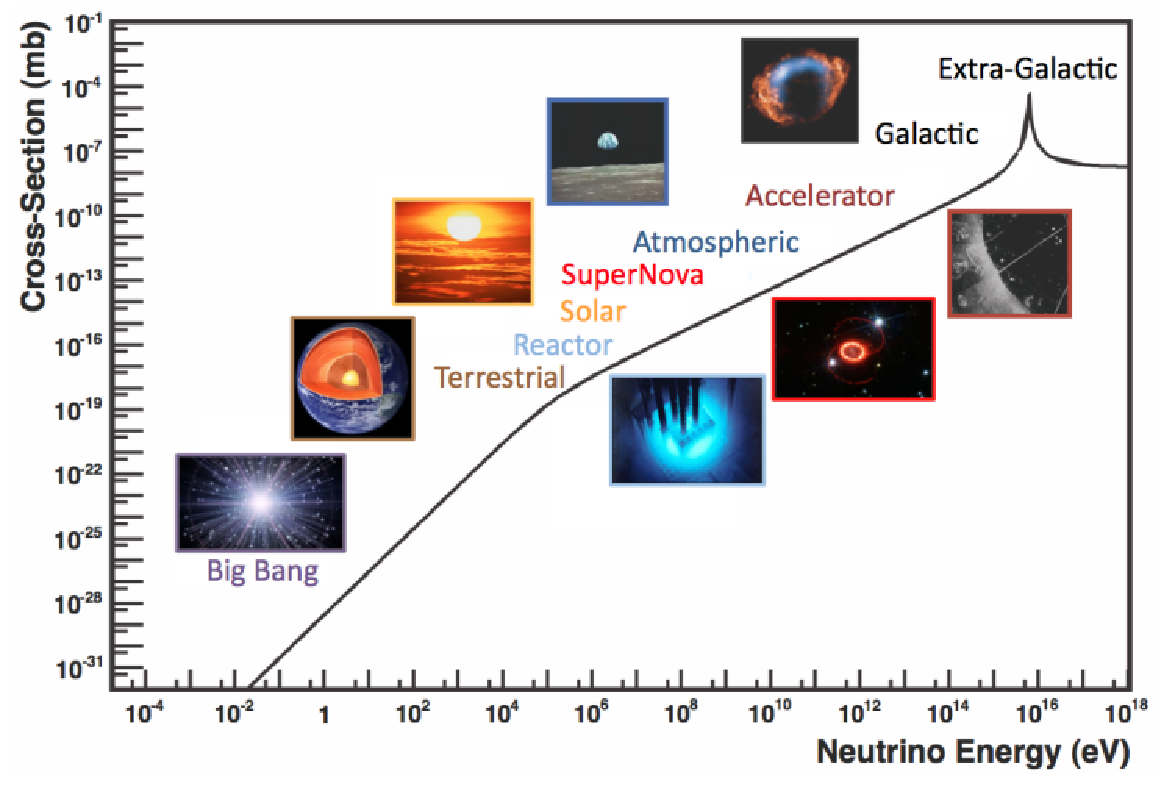
\includegraphics[width=\textwidth, trim={0mm 0mm 0mm 0mm}, clip,page=1]{Figures/Theory/EnergySpectrum.pdf}
  \end{subfigure}
  \caption{The electro-weak cross-section for \quickmath{\bar{\nu_{e}} + e^{-} \rightarrow \bar{\nu_{e}} + e^{-}} scattering on free electrons from various natural and man-made neutrino sources, as a function of neutrino energy. Taken from \cite{Formaggio:2012cpf}.}
  \label{fig:NeutrinoOscillationPhysics_EnergySpectrum}
\end{figure}

\subsection{Solar Neutrinos}
\label{subsec:NeutrinoOscillationPhysics_SolarNeutrinos}

Solar neutrinos are emitted from fusion reaction chains at the centre of the Sun. The solar neutrino flux, given as a function of neutrino energy for different fusion and decay chains, is illustrated in \autoref{fig:NeutrinoOscillationPhysics_SolarNeutrinoFlux}. Whilst proton-proton fusion generates the largest flux of neutrinos, the neutrinos are low energy and are difficult to reconstruct due to the IBD interaction threshold of \quickmath{1.8\text{MeV}} \cite{Oralbaev_2016}. Consequently, most experiments focus on the neutrinos from the decay of \quickmath{^{8}B} (via \quickmath{^{8}B \rightarrow ^{8}Be^{*} + e^{+} + \nu_{e}}), which are higher energy.

\begin{figure}[h]
  \begin{subfigure}[t]{0.80\textwidth}
    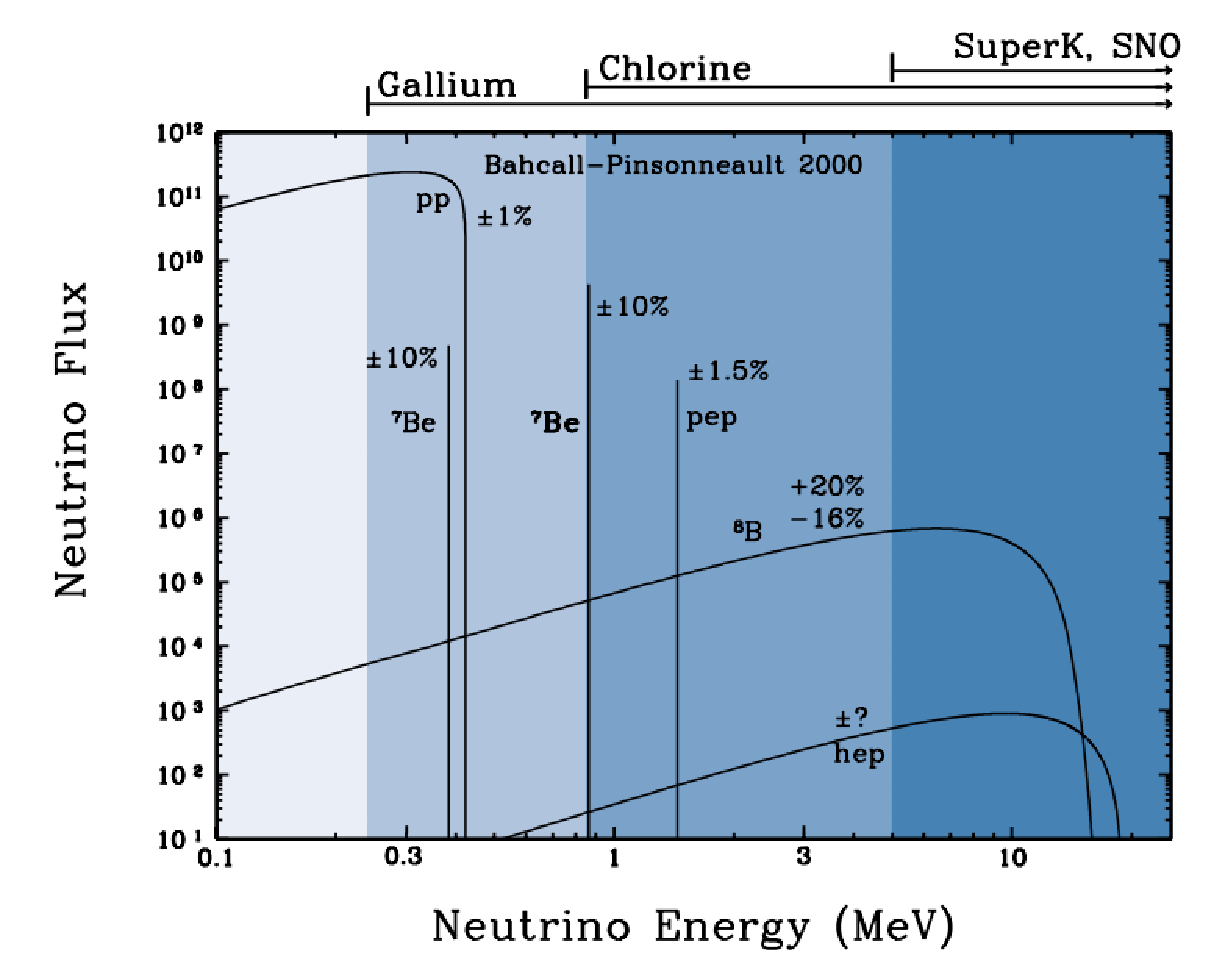
\includegraphics[width=\textwidth, trim={0mm 0mm 0mm 0mm}, clip,page=1]{Figures/Theory/SolarNeutrinoFlux.pdf}
  \end{subfigure}
  \caption{The solar neutrino flux as a function of neutrino energy for various fusion reactions and decay chains as predicted by the Standard Solar Model. Taken from \cite{Bellerive2004-ur}.}
  \label{fig:NeutrinoOscillationPhysics_SolarNeutrinoFlux}
\end{figure}

The first measurements of solar neutrinos observed a significant reduction in the event rate compared to predictions from the Standard Solar Model \cite{PhysRevLett.20.1205, Vinyoles2017-vv}. A proposed solution to this ``solar neutrino problem'' was \quickmath{\nu_{e} \leftrightarrow \nu_{\mu}} oscillations in a precursory version of the PMNS model \cite{Gribov1969-xi}. The Kamiokande \cite{PhysRevLett.63.16}, Gallex \cite{Hampel1999-of} and Sage \cite{PhysRevC.60.055801} experiments confirmed the \quickmath{\sim 0.5} factor deficit of solar neutrinos.

The conclusive solution to this problem was determined by the SNO collaboration \cite{PhysRevLett.89.011301}. Using a deuterium water target to observe \quickmath{^{8}B} neutrinos, the event rate of charged current (CC), neutral current (NC), and elastic scattering (ES) interactions (given in \autoref{eq:NeutrinoOscillationPhysics_SNOInteractions}) was simultaneously measured. CC events can only occur for electron neutrinos, whereas the NC channel is agnostic to neutrino flavour, and the ES channel has a small excess sensitivity for the detection of electron neutrino interactions. This meant that there were direct measurements of the \quickmath{\nu_{e}} and \quickmath{\nu_x} neutrino flux. It was concluded that the CC and ES interaction rates were consistent with the deficit previously observed. Most importantly, the NC reaction rate was only consistent with the others under the hypothesis of flavour transformation.

\begin{equation}
  \label{eq:NeutrinoOscillationPhysics_SNOInteractions}
  \begin{split}
    \nu_{e} + d &\rightarrow p + p + e^{-} \hspace{2cm} (CC) \\
    \nu_{x} + d &\rightarrow p + n + \nu_{x} \hspace{2.02cm} (NC) \\
    \nu_{x} + e^{-} &\rightarrow \nu_{x} + e^{-} \hspace{2.55cm} (ES)
  \end{split}
\end{equation}

%Since the SNO measurement, many experiments have since measured the neutrino flux of different interaction chains within the sun \cite{Borexino_Collaboration2018-of, Aharmim2006-yb, Agostini2020-so}. The most recent measurement was that of CNO-cycle neutrinos which were recently observed with \quickmath{5\sigma} significance by the Borexino collaboration \cite{Borexino_Collaboration2018-of}.
%Future neutrino experiments aim to further these spectroscopic measurements of different fusion chains within the Sun \cite{Andringa2016-zd, Beacom2017-ff, An2016-gm}. %Solar neutrinos act as an irreducible background for dark matter experiments like DARWIN but oscillation parameter measurements can be made \cite{aalbers2020solar}.

\subsection{Accelerator Neutrinos}
\label{subsec:NeutrinoOscillationPhysics_AcceleratorNeutrinos}

The concept of using an artificial ``neutrino beam'' was first realised in 1962 \cite{PhysRevLett.9.36}.
%and led to the first discovery that \quickmath{\nu_{e}} and \quickmath{\nu_{\mu}} were in fact different particles.
Since then, many experiments have adopted the same fundamental concepts. Typically, a proton beam is aimed at a target producing charged mesons that decay to neutrinos. The mesons can be sign-selected by the use of magnetic focusing horns to generate a neutrino or antineutrino beam.
%Absorbing material and the rock between the target and detector absorb all particles barring the neutrinos.
Pions are the primary mesons that decay and depending on the orientation of the magnetic field, a muon (anti-)neutrino beam is generated via \quickmath{\pi^{+} \rightarrow \mu^{+} + \nu_{\mu}} or \quickmath{\pi^{-} \rightarrow \mu^{-} + \bar{\nu}_{\mu}}. The decay of muons and kaons results in an irreducible intrinsic electron neutrino background. In the Tokai-to-Kamioka (T2K) experiment, this background contamination is \quickmath{O(<1\%)} \cite{PhysRevD.87.012001}. There is also an approximately \quickmath{\sim 5\%} ``wrong-sign'' background of \quickmath{\bar{\nu}_{\mu}} generated via the same decays, when operating in neutrino mode. As the beam is generated by proton interactions (rather than anti-proton interactions), the wrong-sign component in the antineutrino beam is larger when operating in neutrino mode.

Tuning the proton energy in the beam and using beam focusing techniques allows the neutrino energy to be set to a value that maximises the disappearance oscillation probability in the \quickmath{L/E} term in \autoref{eq:NeutrinoOscillationPhysics_PMNS_2FlavourOscProb}.
%As the inital proton beam can be tuned resulting in a tunable neutrino energy spectra, the advantage of these type of experiments is that they can be focused in on the oscillation dip presented by the \quickmath{L/E} term in \autoref{eq:NeutrinoOscillationPhysics_PMNS_2FlavourOscProb} using the two flavour approximation.
This means that accelerator experiments are typically more sensitive to the mixing parameters as compared to a natural neutrino source. However, the disadvantage compared to atmospheric neutrino experiments is the cost of building a facility to provide high-energy neutrinos, with a high flux, which is required for longer baselines. Consequently, there is typically less sensitivity to matter effects and the ordering of the neutrino mass eigenstates.

A neutrino experiment measures

\begin{equation}
  \label{eq:NeutrinoOscillationPhysics_DetectorMeasurement}
  R(\vec{x}) = \Phi(E_{\nu}) \times \sigma(E_{\nu}) \times \epsilon(\vec{x}) \times P(\nu_{\alpha} \rightarrow \nu_{\beta}),
\end{equation}

where \quickmath{R(\vec{x})} is the event rate of neutrinos at position \quickmath{\vec{x}}, \quickmath{\Phi(E_{\nu})} is the flux of neutrinos with energy \quickmath{E_{\nu}}, \quickmath{\sigma(E_{\nu})} is the cross-section of the neutrino interaction and \quickmath{\epsilon(\vec{x})} is the efficiency and resolution of the detector. In order to leverage the most out of an accelerator neutrino experiment, the flux and cross-section systematics need to be constrained. This is typically done via the use of a ``near detector'', situated at a baseline of \quickmath{O(1)\text{km}}. This detector observes the unoscillated neutrino flux and constrains the parameters used within the flux and cross-section model.

The first accelerator experiments to precisely measure oscillation parameters were MINOS \cite{PhysRevLett.97.191801} and K2K \cite{k2k_obs}.
These experiments confirmed the \quickmath{\nu_{\mu}} disappearance seen in atmospheric neutrino experiments by finding consistent parameter values for \quickmath{\sin^{2}(\theta_{23})} and \quickmath{\Delta m^{2}_{32}}.
The current generation of accelerator neutrino experiments, T2K and \quickmath{\text{NO}\nu\text{A}} extended this field by observing \quickmath{\bar{\nu}_{\mu} \rightarrow \bar{\nu}_{e}} oscillations and lead the sensitivity to atmospheric mixing parameters as seen in \autoref{fig:NeutrinoOscillationPhysics_AtmosphericParamContour} \cite{PhysRevLett.123.151803}.
The two experiments differ in their peak neutrino energy, baseline, and detection technique.
The \quickmath{\text{NO}\nu\text{A}} experiment is situated at a baseline of \quickmath{810\text{km}} from the NuMI beamline which delivers \quickmath{2\text{GeV}} neutrinos.
The T2K neutrino beam is peaked around \quickmath{0.6 \text{GeV}} and propagates \quickmath{295\text{km}} \cite{t2k_det}.
Additionally, the \quickmath{\text{NO}\nu\text{A}} experiment uses functionally identical detectors (near and far) whereas T2K uses a plastic scintillator technique at the near detector and a water Cherenkov far detector.
The future generation experiments DUNE \cite{Abi2020-cm} and Hyper-Kamiokande \cite{Hyper-Kamiokande_Proto-Collaboration2015-ac} will succeed these experiments as the high-precision era of neutrino oscillation parameter measurements develops.

Several anomalous results have been observed in the LSND \cite{PhysRevD.64.112007} and MiniBooNE \cite{PhysRevLett.110.161801} detectors which were designed with purposefully short baselines. Parts of the neutrino community attributed these results to oscillations induced by a fourth ``sterile'' neutrino \cite{Blanco_2020} but several searches in other experiments, MicroBooNE \cite{10.48550/arxiv.2110.14054} and KARMEN \cite{PhysRevD.65.112001}, found no hints of additional neutrino species. The solution to these anomalous results is still being determined.

\subsection{Atmospheric Neutrinos}
\label{subsec:NeutrinoOscillationPhysics_AtmosphericNeutrinos}

The interactions of primary cosmic ray protons in the Earth's upper atmosphere generate showers of energetic hadrons. These are mostly pions and kaons that decay to produce a natural source of neutrinos spanning energies of MeV to TeV \cite{Gaisser2002-gl}. The main decay is via,

\begin{equation}
  \label{eq:NeutrinoOscillationPhysics_PionDecay}
  \begin{split}
    \pi^{\pm} &\rightarrow \mu^{\pm} + (\nu_{\mu},\bar{\nu}_\mu), \\
    \mu^{\pm} &\rightarrow e^{\pm} + (\nu_{\mu},\bar{\nu}_\mu) + (\nu_{e},\bar{\nu}_e),
  \end{split}
\end{equation}

such that for a single pion decay, three neutrinos can be produced. The atmospheric neutrino flux energy spectra as predicted by the Bartol \cite{Barr_2004}, Honda \cite{Honda_2007, PhysRevD.70.043008, Honda:2011}, and FLUKA \cite{etde_20239111} models are illustrated in \autoref{fig:NeutrinoOscillationPhysics_AtmosphericNeutrinoFlux}. The flux distribution peaks at an energy of \quickmath{O(10) \text{GeV}}. The uncertainties associated with these models are dominated by the hadronic production of kaon and pions as well as the primary cosmic flux. 

\begin{figure}[h]
  \begin{subfigure}[t]{0.80\textwidth}
    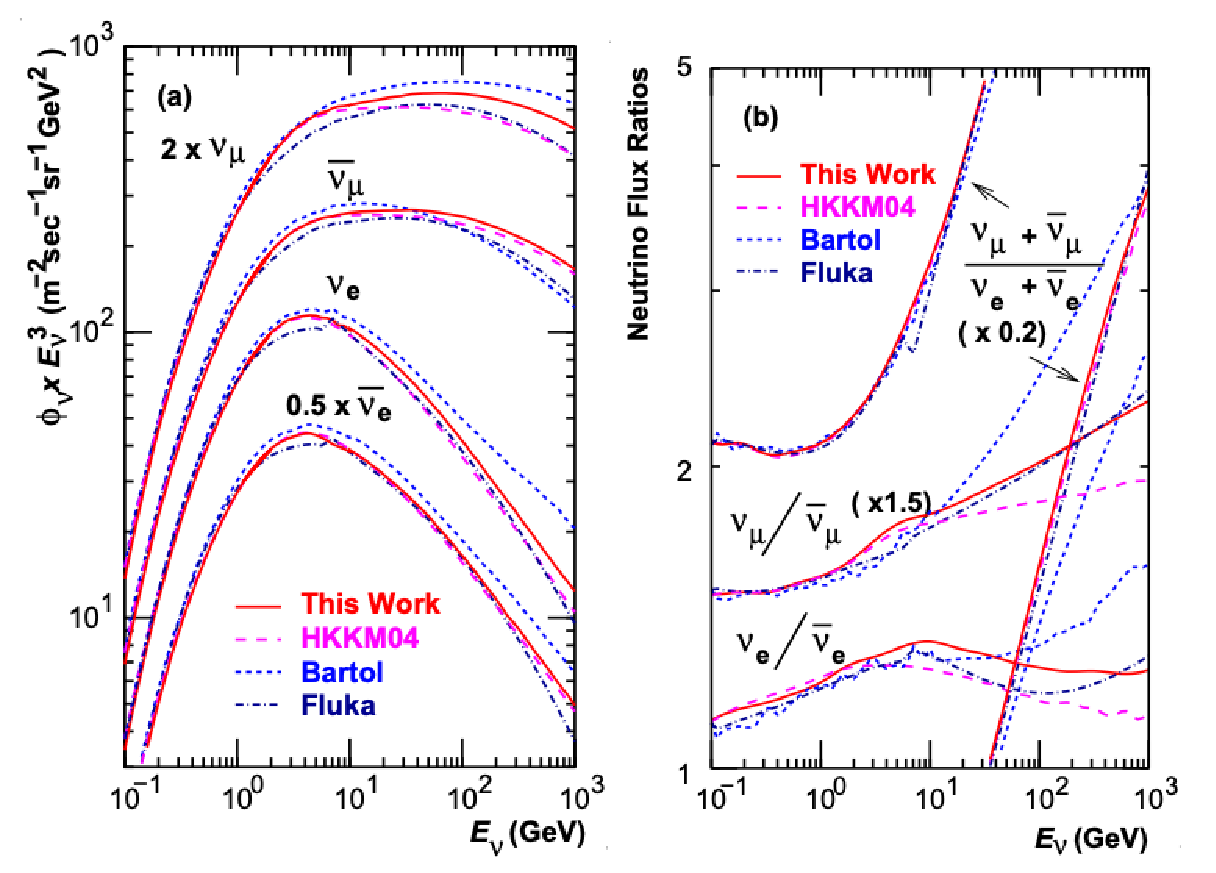
\includegraphics[width=\textwidth, trim={0mm 0mm 0mm 0mm}, clip,page=1]{Figures/Theory/AtmosphericNuFlux.pdf}
  \end{subfigure}
  \caption{Left panel: The atmospheric neutrino flux for different neutrino flavours as a function of neutrino energy as predicted by the 2007 Honda model (``This work'') \cite{Honda_2007}, the 2004 Honda model (``HKKM04'')\cite{PhysRevD.70.043008}, the Bartol model \cite{Barr_2004} and the FLUKA model \cite{etde_20239111}. Right panel: The ratio of the muon to electron neutrino flux as predicted by all the quoted models. Both figures taken from \cite{Honda_2007}.}
  \label{fig:NeutrinoOscillationPhysics_AtmosphericNeutrinoFlux}
\end{figure}

Unlike long-baseline experiments which have a fixed baseline, the distance atmospheric neutrinos propagate is dependent upon the zenith angle, relative to the detector, at which they interact. This is illustrated in \autoref{fig:NeutrinoOscillationPhysics_ZenithAngle}. Neutrinos that are generated directly above the detector (\quickmath{\cos(\theta)=1.0}) have a baseline equivalent to the height of the atmosphere, whereas neutrinos that interact directly below the detector (\quickmath{\cos(\theta)=-1.0}) have to travel a length equal to the diameter of the  Earth. This means atmospheric neutrinos have a baseline that varies from \quickmath{O(20)\text{km}} to \quickmath{O(6 \times 10^{3})\text{km}}. Any neutrino generated at or below the horizon will be subject to MSW matter resonance as they propagate through the Earth.

\begin{figure}[h]
  \begin{subfigure}[t]{0.40\textwidth}
    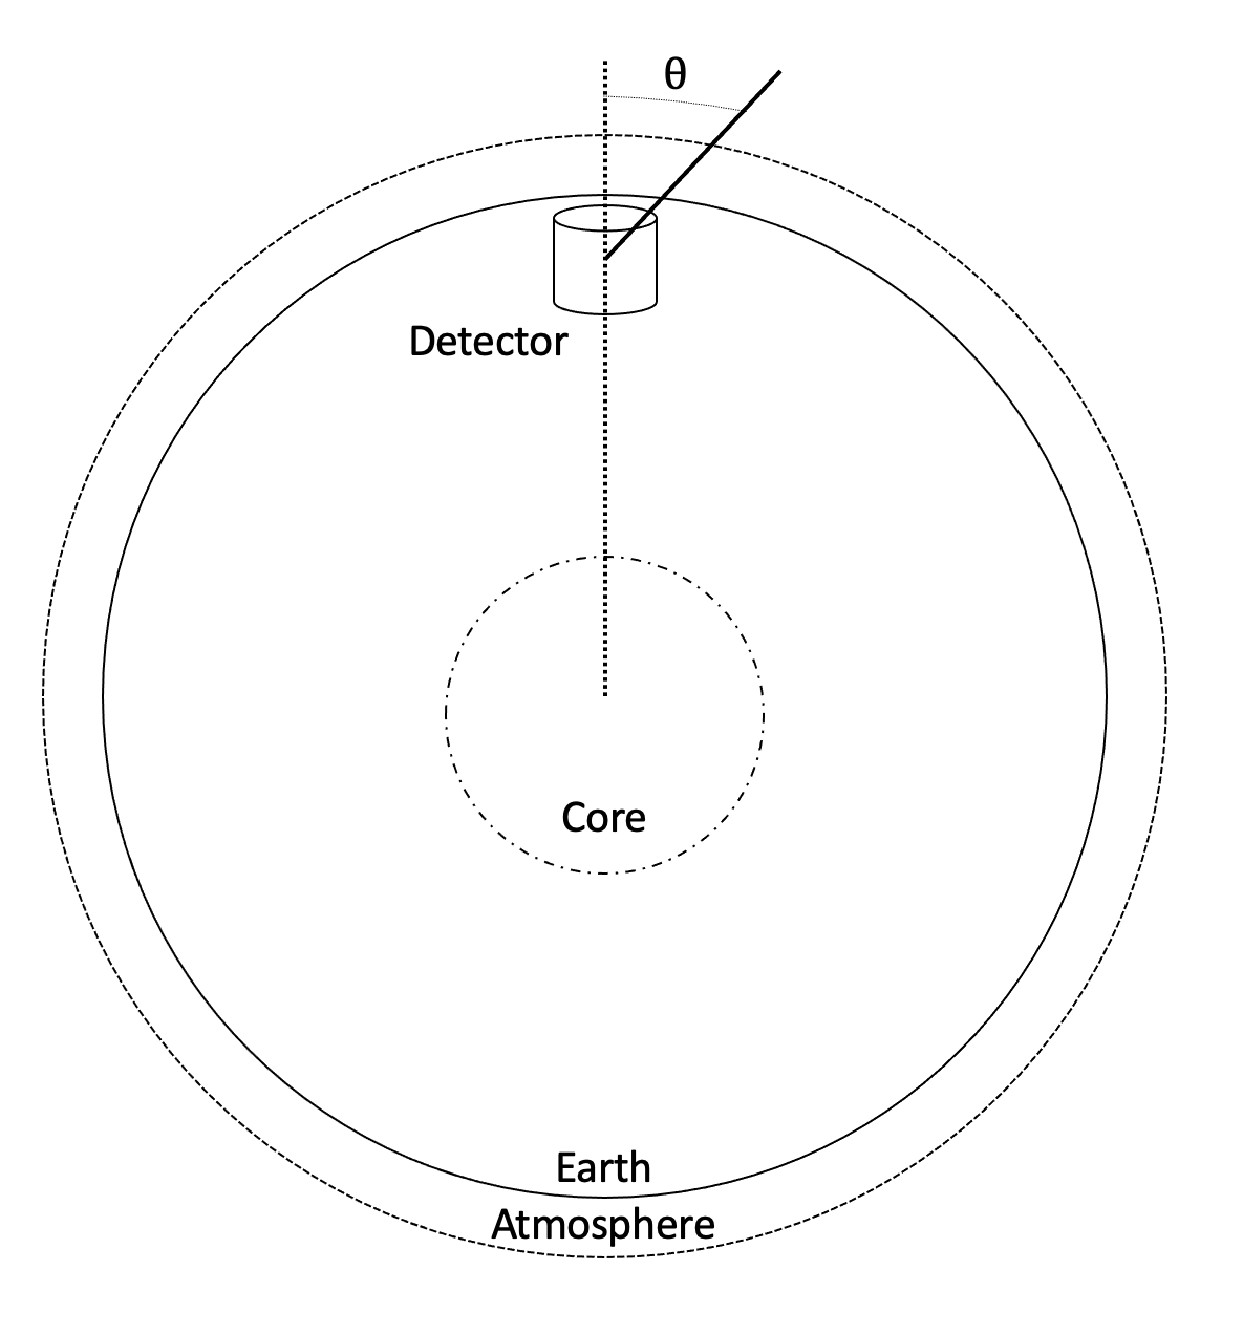
\includegraphics[width=\textwidth, trim={0mm 0mm 0mm 0mm}, clip,page=1]{Figures/Theory/ZenithAngle.pdf}
  \end{subfigure}
  \caption{A diagram illustrating the definition of zenith angle as used in the Super Kamiokande experiment \cite{Ashie_2005}.}
  \label{fig:NeutrinoOscillationPhysics_ZenithAngle}
\end{figure}

\autoref{fig:NeutrinoOscillationPhysics_NuFluxZenithAngleDep} highlights the atmospheric neutrino flux as a function of the zenith angle for different slices of neutrino energy. For medium to high-energy neutrinos (and to a lesser degree for low-energy neutrinos), the flux is approximately symmetric around \quickmath{\cos(\theta)=0}. To the accuracy of this approximation, the systematic uncertainties associated with atmospheric flux for comparing upward-going and down-going neutrino cancels. This allows the down-going events, which are mostly insensitive to oscillation probabilities, to act as an unoscillated prediction (similar to a near detector in an accelerator neutrino experiment).

\begin{figure}[h]
  \begin{subfigure}[t]{0.90\textwidth}
    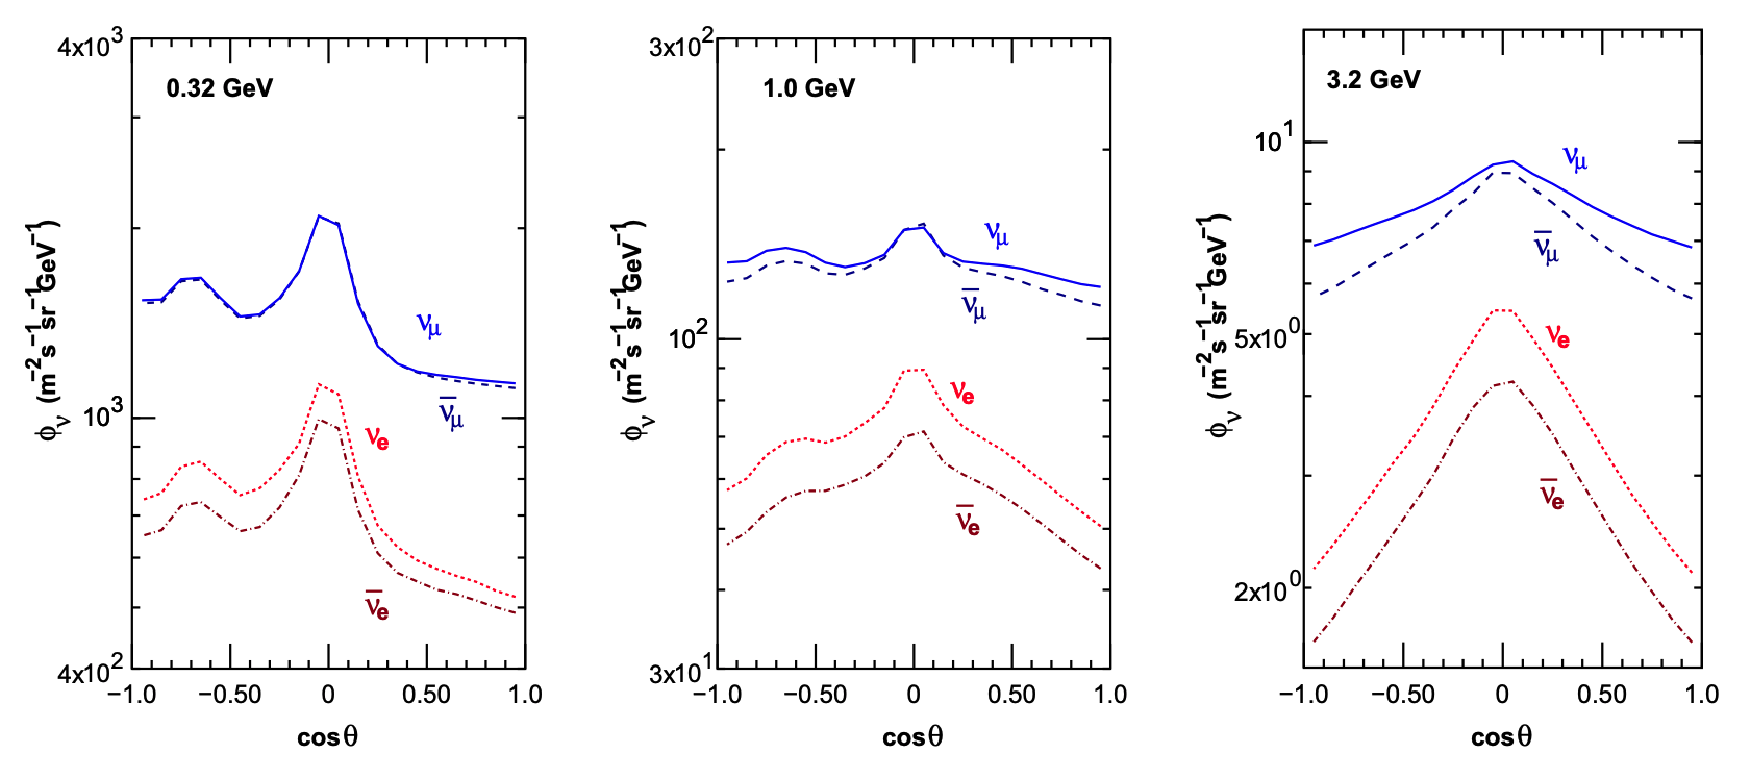
\includegraphics[width=\textwidth, trim={0mm 0mm 0mm 0mm}, clip,page=1]{Figures/Theory/NuFluxZenithAngleDep.pdf}
  \end{subfigure}
  \caption{Prediction of \quickmath{\nu_e, \bar{\nu}_{e}, \nu_{\mu}, \bar{\nu}_{\mu}} fluxes as a function of zenith angle as calculated by the HKKM model \cite{Honda:2011}. The left, middle and right panels represent three values of neutrino energy, \quickmath{0.32\text{GeV}}, \quickmath{1.0\text{GeV}} and \quickmath{3.2\text{GeV}} respectively. Predictions for other models including Bartol \cite{Barr_2004}, Honda \cite{Honda_2007} and FLUKA \cite{etde_20239111} are given in \cite{Ashie_2005}.}
  \label{fig:NeutrinoOscillationPhysics_NuFluxZenithAngleDep}
\end{figure}

Precursory hints of atmospheric neutrinos were observed in the mid-1960s searching for \quickmath{\overset{(-)}{\nu_\mu} + X \rightarrow X^{*} + \mu^{\pm}} \cite{Reines1965-cf}.
%, although it was called an anomaly at the time of measurement.
This was succeeded by the IMB-3 \cite{PhysRevLett.66.2561} and Kamiokande \cite{Hirata1992-qz} experiments which measured the double ratio of muon to electron neutrinos in data to Monte Carlo, \quickmath{R(\nu_{\mu}/\nu_{e}) = (\mu/e)_{Data}/(\mu/e)_{MC}}. Both experiments were found to have a consistent deficit of muon neutrinos, with \quickmath{R(\nu_{\mu}/\nu_{e}) = 0.67 \pm 0.17} and \quickmath{R(\nu_{\mu}/\nu_{e}) = 0.658 \pm 0.016 \pm 0.035}, respectively. %Soudan-2 \cite{Allison1997-qz} determined similar measurements.
Super-Kamiokande (SK) \cite{Ashie_2005} extended this analysis by fitting oscillation parameters in \quickmath{P(\nu_\mu \rightarrow \nu_\tau)} which found best fit parameters \quickmath{\sin^{2}(2\theta) > 0.92} and \quickmath{1.5 \times 10^{-3} < \Delta m^{2} < 3.4 \times 10^{-3} \text{eV}^{2}}.

Since then, atmospheric neutrino experiments have been making precision measurements of the \quickmath{\sin^{2}(\theta_{23})} and \quickmath{\Delta m^{2}_{32}} oscillation parameters.
%, and to a lesser extent the sign of \quickmath{\Delta m^{2}_{32}} through the matter resonance present for any neutrinos passing through the Earth.
Atmospheric neutrino oscillation is dominated by \quickmath{P(\nu_{\mu} \rightarrow \nu_{\tau})}, where SK observed a \quickmath{4.6\sigma} discovery of \quickmath{\nu_{\tau}} appearance \cite{Li_2018}. \autoref{fig:NeutrinoOscillationPhysics_AtmosphericParamContour} illustrates the current estimates on the atmospheric mixing parameters, from a wide range of atmospheric and accelerator neutrino observatories.

\begin{figure}[h]
  \begin{subfigure}[t]{0.90\textwidth}
    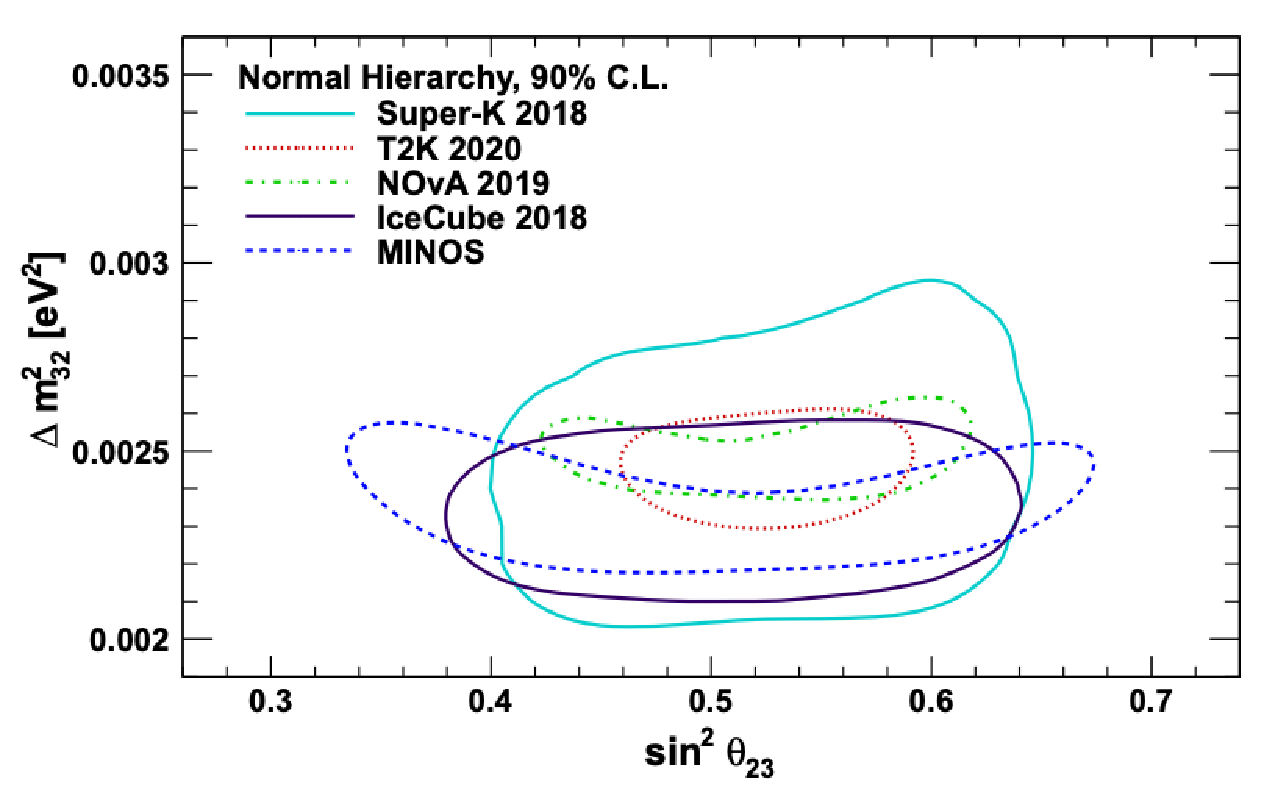
\includegraphics[width=\textwidth, trim={0mm 0mm 0mm 0mm}, clip,page=1]{Figures/Theory/AtmosphericParams.pdf}
  \end{subfigure}
  \caption{Constraints on the atmospheric oscillation parameters, \quickmath{\sin^{2}(\theta_{23})} and \quickmath{\Delta m^{2}_{32}}, from atmospheric and long-baseline experiments: SK \cite{Kamiokande_Collaboration2017-nf}, T2K \cite{T2K_Collaboration2018-sm}, \quickmath{\text{NO}\nu\text{A}} \cite{Acero2019-rw}, IceCube \cite{Aartsen2018-cz} and MINOS \cite{Adamson2014-tt}. Figure taken from \cite{Athar_2022}.}
  \label{fig:NeutrinoOscillationPhysics_AtmosphericParamContour}
\end{figure}

\subsection{Reactor Neutrinos}
\label{subsec:NeutrinoOscillationPhysics_ReactorNeutrinos}

As illustrated in the first discovery of neutrinos (\autoref{sec:NeutrinoOscillationPhysics_Discovery}), nuclear reactors are a very useful artificial source of electron antineutrinos. For reactors that use low-enriched uranium \quickmath{^{235}\text{U}} as fuel, the antineutrino flux is dominated by the \quickmath{\beta}-decay fission of \quickmath{^{235}\text{U}}, \quickmath{^{238}\text{U}}, \quickmath{^{239}\text{Pu}} and \quickmath{^{241}\text{Pu}} \cite{Kim2013-ye} as illustrated in \autoref{fig:NeutrinoOscillationPhysics_ReactorNeutrinoProduction}.

\begin{figure}[h]
  \begin{subfigure}[t]{0.90\textwidth}
    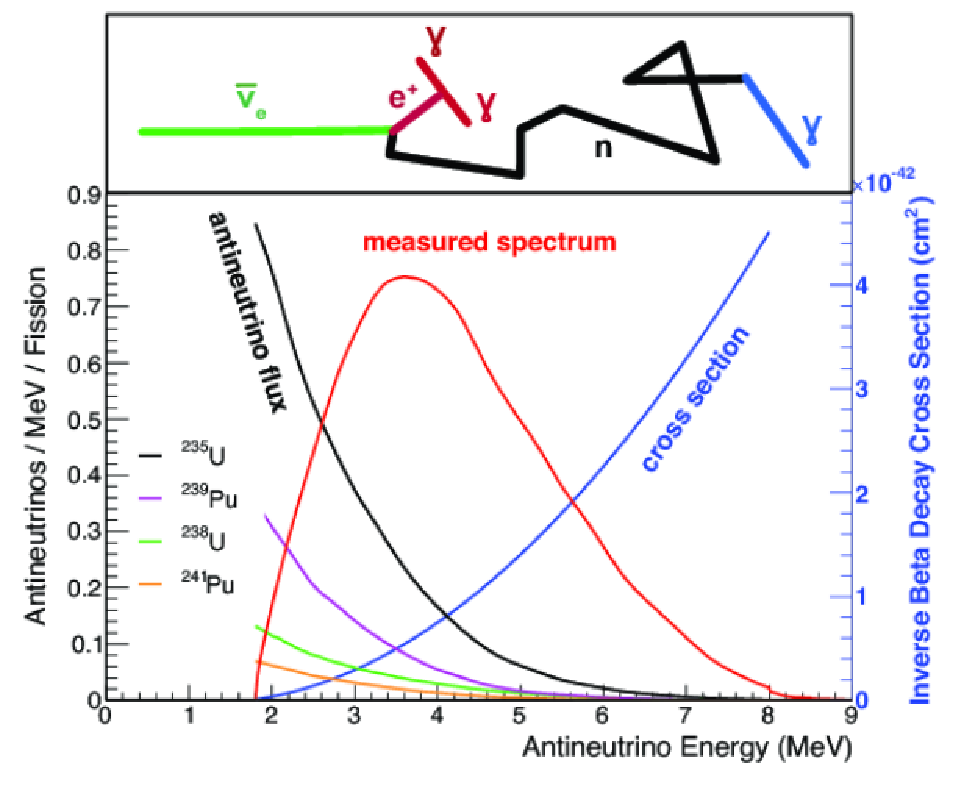
\includegraphics[width=\textwidth, trim={0mm 0mm 0mm 0mm}, clip,page=1]{Figures/Theory/ReactorNeutrinoProduction.pdf}
  \end{subfigure}
  \caption{Reactor electron antineutrino fluxes for \quickmath{^{235}\text{U}} (Black), \quickmath{^{238}\text{U}} (Green), \quickmath{^{239}\text{Pu}} (Purple), and \quickmath{^{241}\text{Pu}} (Orange) isotopes. The inverse \quickmath{\beta}-decay cross-section (Blue) and corresponding measurable neutrino spectrum (Red) are also given. Top panel: Schematic of Inverse \quickmath{\beta}-decay interaction including the eventual capture of the emitted neutron. This capture emits a \quickmath{\gamma}-ray which provides a second signal of the event. Taken from \cite{Athar_2022}.}
  \label{fig:NeutrinoOscillationPhysics_ReactorNeutrinoProduction}
\end{figure}

Due to their low energy, reactor electron antineutrinos predominantly interact via the inverse \quickmath{\beta}-decay (IBD) interaction. The typical signature contains two signals delayed by \quickmath{O(200)\mu\text{s}}; firstly the prompt photons from positron annihilation, and secondly the photon emitted (\quickmath{E_{tot}^{\gamma} = 2.2\text{MeV}}) from de-excitation after neutron capture on hydrogen. Searching for both signals improves the detector's ability to distinguish between background and signal events \cite{Abe2022-ij}. %Recently, SK included gadolinium dopants into the ultra-pure water to increase the energy released from the photon cascade to \quickmath{\sim 8\text{MeV}} and reduce the time of the delayed signal to \quickmath{\sim 28 \mu \text{s}}.

There are many short baseline experiments (\quickmath{\text{L} \sim O(1)\text{km}}) that have measured the \quickmath{\sin^{2}(\theta_{13})} and \quickmath{\Delta m^{2}_{32}} oscillation parameters. Daya Bay \cite{PhysRevLett.108.171803}, RENO \cite{PhysRevLett.108.191802} and Double Chooz \cite{PhysRevLett.108.131801} have all provided precise measurements, with the first discovery of a non-zero \quickmath{\theta_{13}} made by Daya Bay and RENO (and complemented by T2K \cite{PhysRevLett.108.131801}). The constraints on \quickmath{\sin^{2}(\theta_{13})} by the reactor experiments lead the field. They are often used as external inputs to accelerator neutrino experiments to improve their sensitivity to \quickmath{\delta_{CP}} and mass hierarchy determination.
%One curiosity of these short baseline reactor experiments is the `\quickmath{5 \text{MeV}} excess' \cite{Berryman_2019}. First observed in 2014 \cite{For_the_RENO_Collaboration2015-zy, Abe_2014}, all three experiments listed observed a shape excess in events around \quickmath{E_{\nu} \sim 5 \text{MeV}}. The reason behind this excess is speculated to be either oscillations to sterile neutrinos or a fault in the Huber-Mueller model \cite{Mueller_2011}. At this time, the latter is favoured as Daya Bay \cite{PhysRevLett.123.111801} observed substantial evidence (\quickmath{4.0\sigma}) of correlation between the excess and the \quickmath{^{235}\text{U}} electron antineutrino flux.
%Other neutrino experiments, PROSPECT \cite{PhysRevD.103.032001} and STEREO \cite{STEREO} show similar results data to help determine the cause of the excess.
%JUNO-TAO \cite{junocollaboration2020tao}, a small collaboration within the larger JUNO experiment, is a next-generation reactor experiment that aims to precisely measure the isotopic antineutrino yields from the different fission chains. %Alongside this, it aims to explain the `\quickmath{5 \text{MeV}} excess' of neutrino events observed by other reactor neutrino experiments \cite{For_the_RENO_Collaboration2015-zy, Abe_2014, PhysRevLett.123.111801}. It does this by conducting a search for sterile neutrinos with a mass scale of around \quickmath{1 \text{eV}}.

Kamland \cite{Decowski2016-hh} is the only experiment to have observed reactor neutrinos using a long baseline (flux weighted averaged baseline of \quickmath{L \sim 180\text{km}}) which allows it to have sensitivity to \quickmath{\Delta m^{2}_{21}}. Combined with the SK solar neutrino experiment, the combined analysis puts the most stringent constraint on \quickmath{\Delta m^{2}_{21}} \cite{PhysRevD.83.052002}.

\section{Summary Of Oscillation Parameter Measurements}
\label{sec:Theory_Summary}

Since the first evidence of neutrino oscillations, numerous measurements of the mixing parameters have been made. Many experiments use neutrinos as a tool for the discovery of new physics (diffuse supernova background, neutrinoless double beta decay and others) so the PMNS parameters are summarised in the Particle Data Group (PDG) review tables. The analysis presented in this thesis focuses on the 2020 T2K oscillation analysis presented in \cite{Dunne2020-uf} which uses the 2020 PDG constraints \cite{Particle_Data_Group2020-ms}. These constraints are outlined in \autoref{tab:Theory_PDGConstraints}.

\begin{table}[ht!]
    \centering
    \begin{tabular}{c|c}
      \hline
      Parameter & 2020 Constraint \\
      \hline
      \quickmath{\sin^{2}(\theta_{12})} & \quickmath{0.307 \pm 0.013} \\
      \quickmath{\Delta m^{2}_{21}} & \quickmath{(7.53 \pm 0.18) \times 10^{-5} \text{eV}^{2}} \\
      \quickmath{\sin^{2}(\theta_{13})} & \quickmath{(2.18 \pm 0.07) \times 10^{-2}} \\
      \quickmath{\sin^{2}(\theta_{23})} (I.H.) & \quickmath{0.547 \pm 0.021} \\
      \quickmath{\sin^{2}(\theta_{23})} (N.H.) & \quickmath{0.545 \pm 0.021} \\
      \quickmath{\Delta m^{2}_{32}} (I.H.) & \quickmath{(-2.546^{+0.034}_{-0.040}) \times 10^{-3} \text{eV}^{2}} \\
      \quickmath{\Delta m^{2}_{32}} (N.H.) & \quickmath{(2.453\pm0.034) \times 10^{-3} \text{eV}^{2}} \\
      \hline
      \hline
    \end{tabular}
    \caption{The 2020 Particle Data Group constraints of the oscillation parameters taken from \cite{Particle_Data_Group2020-ms}. The value of \quickmath{\Delta m^{2}_{32}} is given for both normal hierarchy (N.H.) and inverted hierarchy (I.H.) and \quickmath{\sin^{2}(\theta_{23})} is broken down by whether its value is below (Q1) or above (Q2) \quickmath{0.5}.}
    \label{tab:Theory_PDGConstraints}
\end{table}

The \quickmath{\sin^{2}(\theta_{13})} measurement stems from the electron antineutrino disappearance, \quickmath{P(\bar{\nu}_{e} \rightarrow \bar{\nu}_{e})}, and is taken as the  average best-fit from the combination of Daya Bay, Reno and Double Chooz. It is often used as a prior uncertainty within other neutrino oscillation experiments, typically termed the reactor constraint. The \quickmath{\sin^{2}(\theta_{12})} parameter is predominantly measured through electron neutrino disappearance, \quickmath{P(\nu_{e} \rightarrow \nu_{\mu,\tau})}, in solar neutrino experiments. The long-baseline reactor neutrino experiment Kamland also has a sensitivity to this parameter and is used in a joint fit to solar data from SNO and SK, using the reactor constraint. Measurements of \quickmath{\sin^{2}(\theta_{23})} are made by long-baseline and atmospheric neutrino experiments. The PDG value is a joint fit of T2K, \quickmath{\text{NO}\nu\text{A}}, MINOS and IceCube DeepCore experiments. The latest T2K-only measurement, provided at Neutrino2020 and is the basis of this thesis, is given as \quickmath{\sin^{2}(\theta_{23}) = 0.546^{+0.024}_{-0.046}} \cite{Dunne2020-uf}. The PDG constraint on \quickmath{\Delta m^{2}_{21}} is provided by the KamLAND experiment using solar and geoneutrino data. This measurement utilised a \quickmath{\sin^{2}(\theta_{13})} constraint from accelerator (T2K, MINOS) and reactor neutrino (Daya Bay, RENO, Double Chooz) experiments. Accelerator measurements make some of the most stringent constraints on \quickmath{\Delta m^{2}_{32}} although atmospheric experiments have more sensitivity to the mass hierarchy determination. The PDG performs a joint fit of accelerator and atmospheric data, in both normal and inverted hierarchies separately. The latest T2K-only result is \quickmath{\Delta m^{2}_{32} = 2.49^{+0.058}_{-0.082} \times 10^{-3}\text{eV}^{2}} favouring normal hierarchy \cite{Dunne2020-uf}. The value of \quickmath{\delta_{CP}} is largely undetermined. CP-conserving values of \quickmath{0} and \quickmath{\pi} were rejected with \quickmath{\sim 2\sigma} intervals, as published in Nature \cite{Nature2020}.
%, although more recent analyses have reduced the credible intervals to \quickmath{90\%}.
Since the 2020 PDG publication, there has been a new measurement of \quickmath{\sin^{2}(\theta_{13}) = (2.20 \pm 0.07) \times 10^{-2}} \cite{Workman:2022ynf}, alongside updated \quickmath{\Delta m^{2}_{32}} and \quickmath{\sin^{2}(\theta_{23})} measurements.

Throughout this thesis, several sample spectra predictions and contours are presented, which require oscillation parameters to be assumed. \autoref{tab:Theory_ParameterSets} defines two sets of oscillation parameters, with ``Asimov A'' set being close to the preferred values from a previous T2K-only fit \cite{PhysRevLett.112.181801} and ``Asimov B'' being CP-conserving and further from maximal \quickmath{\theta_{23}} mixing.

\begin{table}[ht!]
    \centering
    \begin{tabular}{c|c|c}
      \hline
      \hline
      Parameter & Asimov A & Asimov B \\
      \hline
      \quickmath{\Delta m^{2}_{12}} & \multicolumn{2}{c}{\quickmath{7.53 \times 10^{-5} \text{eV}^{2}}} \\ \hline
      \quickmath{\Delta m^{2}_{32}} & \multicolumn{2}{c}{\quickmath{2.509 \times 10^{-3} \text{eV}^{2}}} \\ \hline
      \quickmath{\sin^{2}\left(\theta_{12}\right)} & \multicolumn{2}{c}{\quickmath{0.304}} \\ \hline
      \quickmath{\sin^{2}\left(\theta_{13}\right)} & \multicolumn{2}{c}{\quickmath{0.0219}} \\ \hline
      \quickmath{\sin^{2}\left(\theta_{23}\right)} & \quickmath{0.528} & \quickmath{0.45} \\ \hline
      \quickmath{\delta_{CP}} & \quickmath{-1.601} & \quickmath{0.0} \\ \hline
      \hline
    \end{tabular}
    \caption{Reference values of the neutrino oscillation parameters for two different oscillation parameter sets.}
    \label{tab:Theory_ParameterSets}
\end{table}

\section{Overview of Oscillation Effects}
\label{sec:Oscillation_Overview}

The analysis presented within this thesis focuses on the determination of oscillation parameters from a joint atmospheric and beam analysis which combines the SK and T2K experiments. Whilst subject to the same oscillation formalism, the way in which the two samples have sensitivity to the different oscillation parameters differs significantly.

Atmospheric neutrinos have a varying baseline, or ``path length'' \quickmath{L}, such that the distance each neutrino travels before interacting is dependent upon the zenith angle, \quickmath{\theta_{Z}}. As primary cosmic rays can interact anywhere between the Earth's surface and \quickmath{\sim50\text{km}} above that, the height, \quickmath{h}, in the atmosphere at which the neutrino was generated also affects the path length,

\begin{equation}
  L = \sqrt{\left(R_{E} + h\right)^{2} - R_{E}^{2} \left(1 - \cos^{2} \left(\theta_{Z} \right) \right)} - R_{E}\cos(\theta_{Z}).
\end{equation}

Where \quickmath{R_{E} = 6,371\text{km}} is the Earth's radius. This assumes a spherically symmetric Earth model. Therefore, the oscillation probability is dependent upon two parameters, \quickmath{\cos(\theta_{Z})} and \quickmath{E_{\nu}}.

The oscillation probability used within this analysis is based on \cite{Barger:1980tf}. The neutrino wavefunction in the vacuum Hamiltonian evolves in each layer of constant matter density via

\begin{equation}
  i \frac{d\psi_{j}(t)}{dt} = \frac{m_{j}^{2}}{2E_{\nu}} \psi_{j}(t) - \sum_{k} \sqrt{2} G_{F} N_{e} U_{ej} U_{ke}^{\dagger} \psi_{k}(t),
\end{equation}

where \quickmath{m_{j}^{2}} is the square of the \quickmath{j^{th}} vacuum eigenstate mass, \quickmath{E_{\nu}} is the neutrino energy, \quickmath{G_{F}} is Fermi's constant, \quickmath{N_{e}} is the electron number density and \quickmath{U} is the PMNS matrix. The transformation \quickmath{N_{e} \rightarrow -N_{e}} and \quickmath{\delta_{CP} \rightarrow -\delta_{CP}} is applied for antineutrino propagation. Thus, a model of the Earth's density is required for neutrino propagation. Following the SK methodology \cite{thesis_roger}, this analysis uses the Preliminary Reference Earth Model (PREM) \cite{Dziewonski1981-sp} which provides piecewise cubic polynomials as a function of the Earth's radius. This density profile is illustrated in \autoref{fig:Oscillation_SK_PREMModelApproximation}. As the propagator requires layers of constant density, the SK methodology approximates the PREM model by using four layers of constant density \cite{thesis_roger}, detailed in \autoref{tab:NeutrinoOscillationPhysics_PREMModel}.

\begin{figure}[h]
  \begin{subfigure}[t]{0.8\textwidth}
    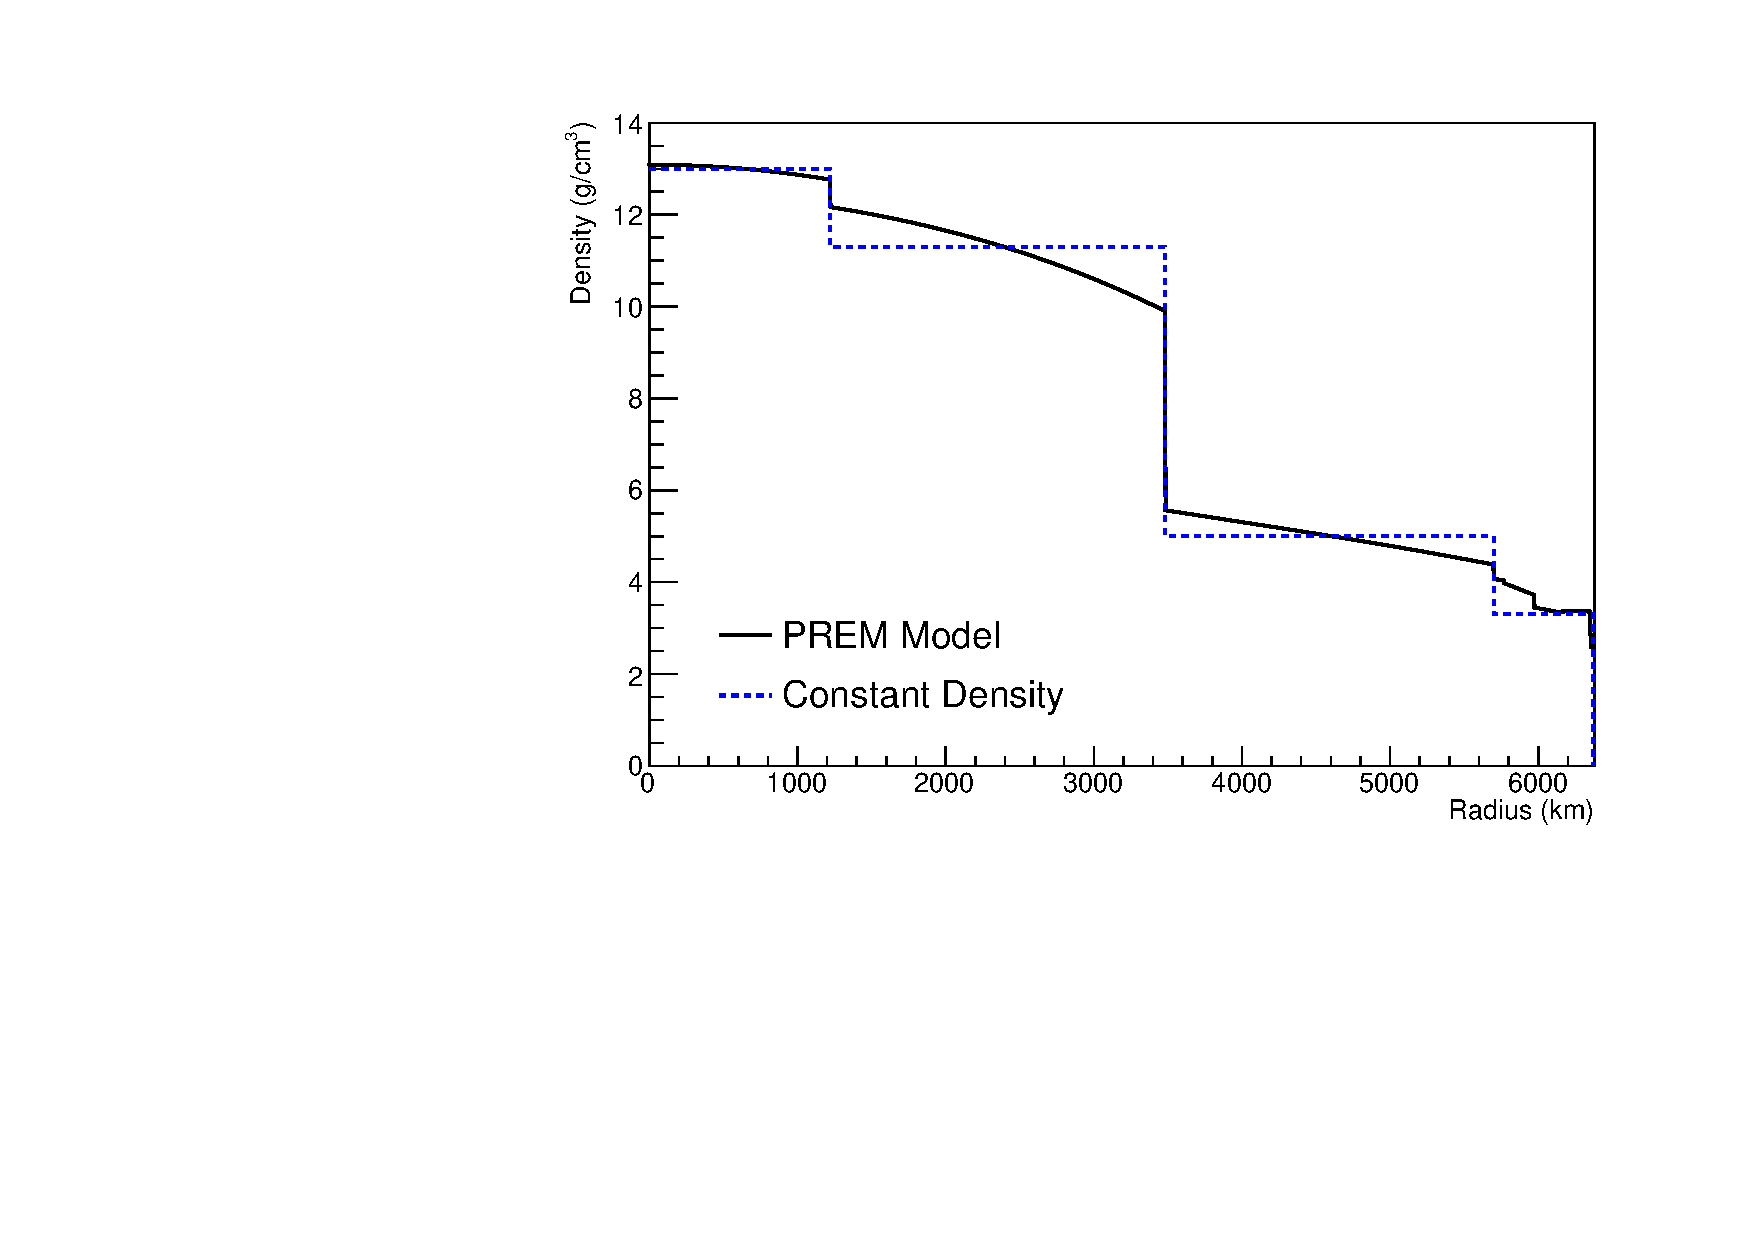
\includegraphics[width=\textwidth, trim={0mm 0mm 0mm 0mm}, clip,page=1]{Figures/Oscillation/DensityComparison.pdf}
  \end{subfigure}
  \caption{The density of the Earth given as a function of the radius, as provided by the PREM model (Black), and the constant density four-layer approximation (Blue), as used in the official SK-only analysis.}
  \label{fig:Oscillation_SK_PREMModelApproximation}
\end{figure}

\begin{table}[ht!]
    \centering
    \begin{tabular}{c|c|c|c}
      \hline
      Layer & Outer Radius [\quickmath{\text{km}}] & Density [\quickmath{\text{g/cm}^{3}}] & Chemical composition (Z/A) \\
      \hline
      Inner Core & \quickmath{1220} & \quickmath{13} & \quickmath{0.468 \pm 0.029} \\
      Outer Core & \quickmath{3480} & \quickmath{11.3} & \quickmath{0.468 \pm 0.029} \\
      Lower Mantle & \quickmath{5701} & \quickmath{5.0} & \quickmath{0.496} \\
      Transition Zone & \quickmath{6371} & \quickmath{3.3} & \quickmath{0.496} \\
      \hline
    \end{tabular}
    \caption{Description of the four layers of the Earth invoked within the constant density approximation of the PREM model \cite{Dziewonski1981-sp}.}
    \label{tab:NeutrinoOscillationPhysics_PREMModel}
\end{table}

The atmospheric neutrino oscillation probabilities can be presented as two dimensional ``oscillograms'' as illustrated in \autoref{fig:Oscillation_SK_BasicOscillogram}. The distinct discontinuities, as a function of \quickmath{\cos(\theta_{Z})}, are due to the discontinuous density in the PREM model.

\begin{figure}[h]
  \begin{subfigure}[t]{0.8\textwidth}
    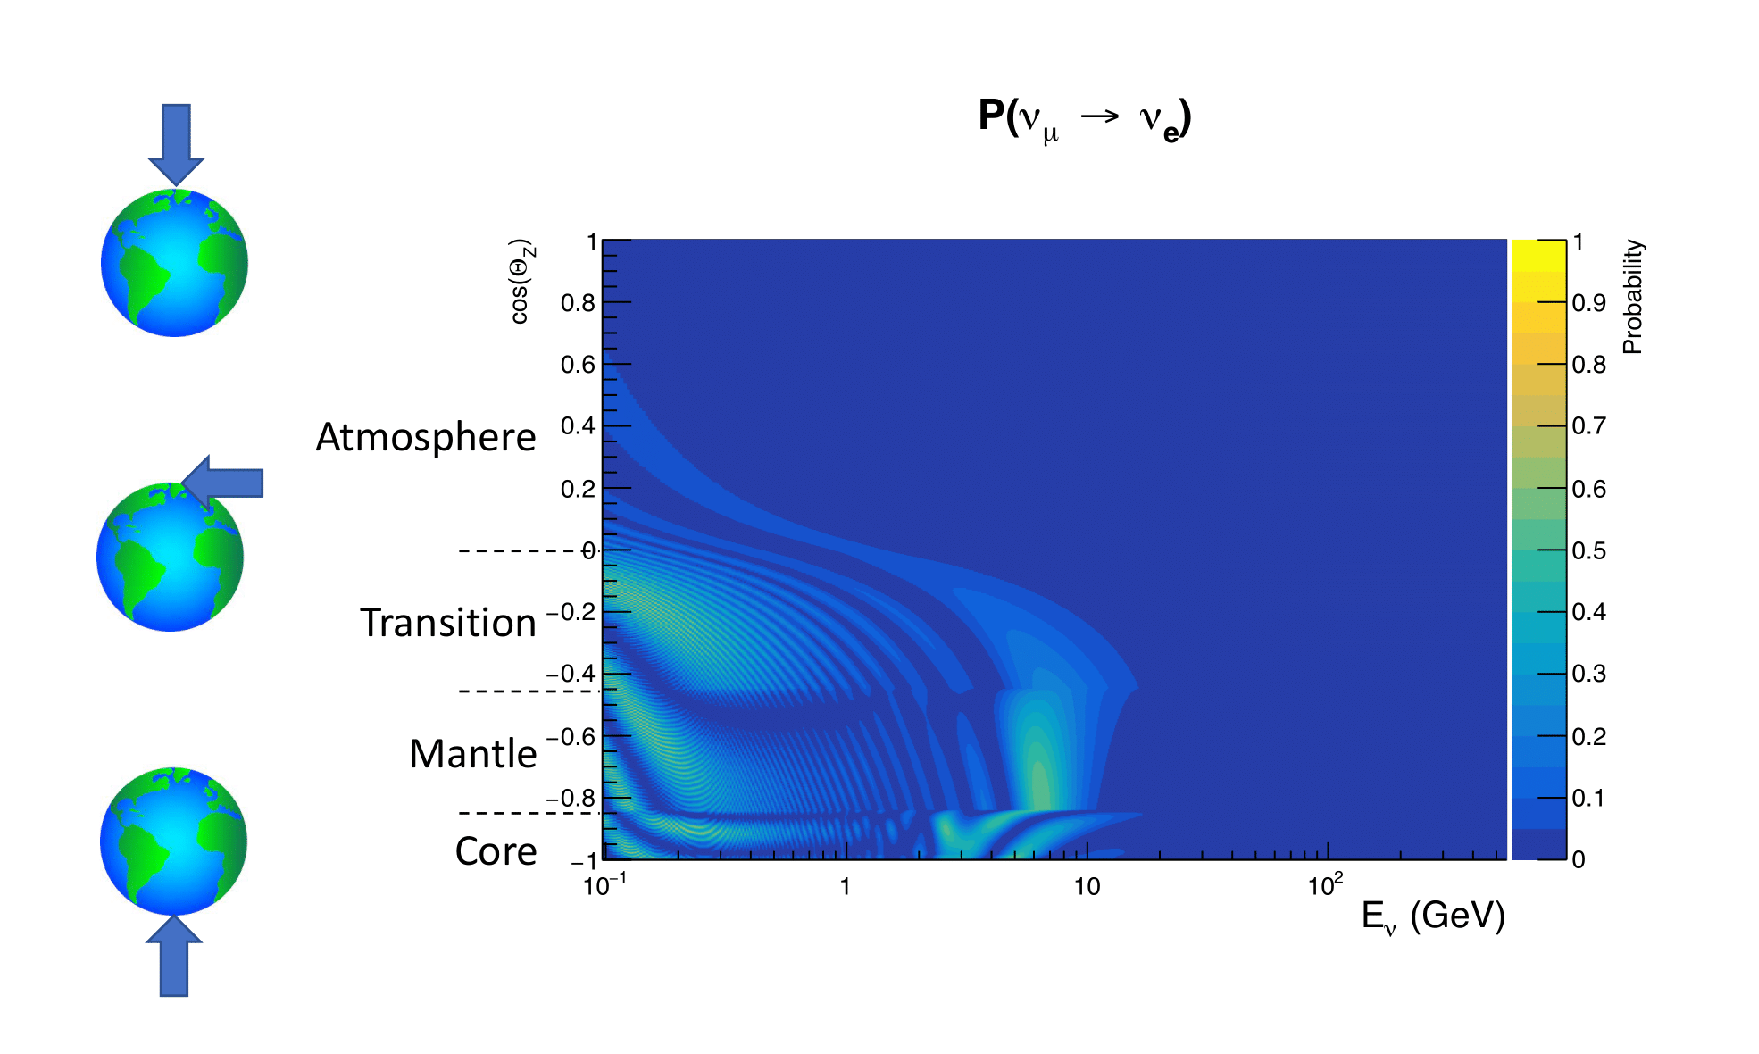
\includegraphics[width=\textwidth, trim={0mm 0mm 0mm 0mm}, clip,page=1]{Figures/Oscillation/BasicOscillogramWithNotes.pdf}
  \end{subfigure}
  \caption{An ``oscillogram'' that depicts the \quickmath{P(\nu_\mu \rightarrow \nu_e)} oscillation probability as a function of neutrino energy and cosine of the zenith angle. The zenith angle is defined such that \quickmath{\cos(\theta_{Z}) = 1.0} represents neutrinos that travel from directly above the detector. The four-layer constant density PREM model approximation is used and Asimov A oscillation parameters are assumed (\autoref{tab:Theory_ParameterSets}).}
  \label{fig:Oscillation_SK_BasicOscillogram}
\end{figure}

Atmospheric neutrinos have sensitivity to \quickmath{\delta_{CP}} through the overall event rate. \autoref{fig:Oscillation_SK_DCPSensitivity} illustrates the difference in oscillation probability between CP-conserving (\quickmath{\delta_{CP} = 0.}) and a CP-violating (\quickmath{\delta_{CP} = -1.601}) value taken from Asimov A oscillation parameter set (\autoref{tab:Theory_ParameterSets}). The result is a complicated oscillation pattern in the appearance probability for sub-GeV upgoing neutrinos. The detector does not have sufficient resolution to resolve these individual patterns so the sensitivity to \quickmath{\delta_{CP}} for atmospheric neutrinos comes via the overall normalisation of these events.

The presence of matter means that the effect \quickmath{\delta_{CP}} has on the oscillation probability is not equal between neutrinos and antineutrinos. Furthermore, the interaction cross-section for neutrinos is larger than for antineutrinos so the two effects have to be disentangled.
%These effects are further convoluted by detector efficiencies as SK cannot distinguish neutrinos and antineutrinos well.
All of these effects lead to a difference in the number of neutrinos detected compared to antineutrinos. This changes how the \quickmath{\delta_{CP}} normalisation term is observed, resulting in a very complex sensitivity to \quickmath{\delta_{CP}}.

\begin{figure}[h]
  \begin{subfigure}[t]{\textwidth}
    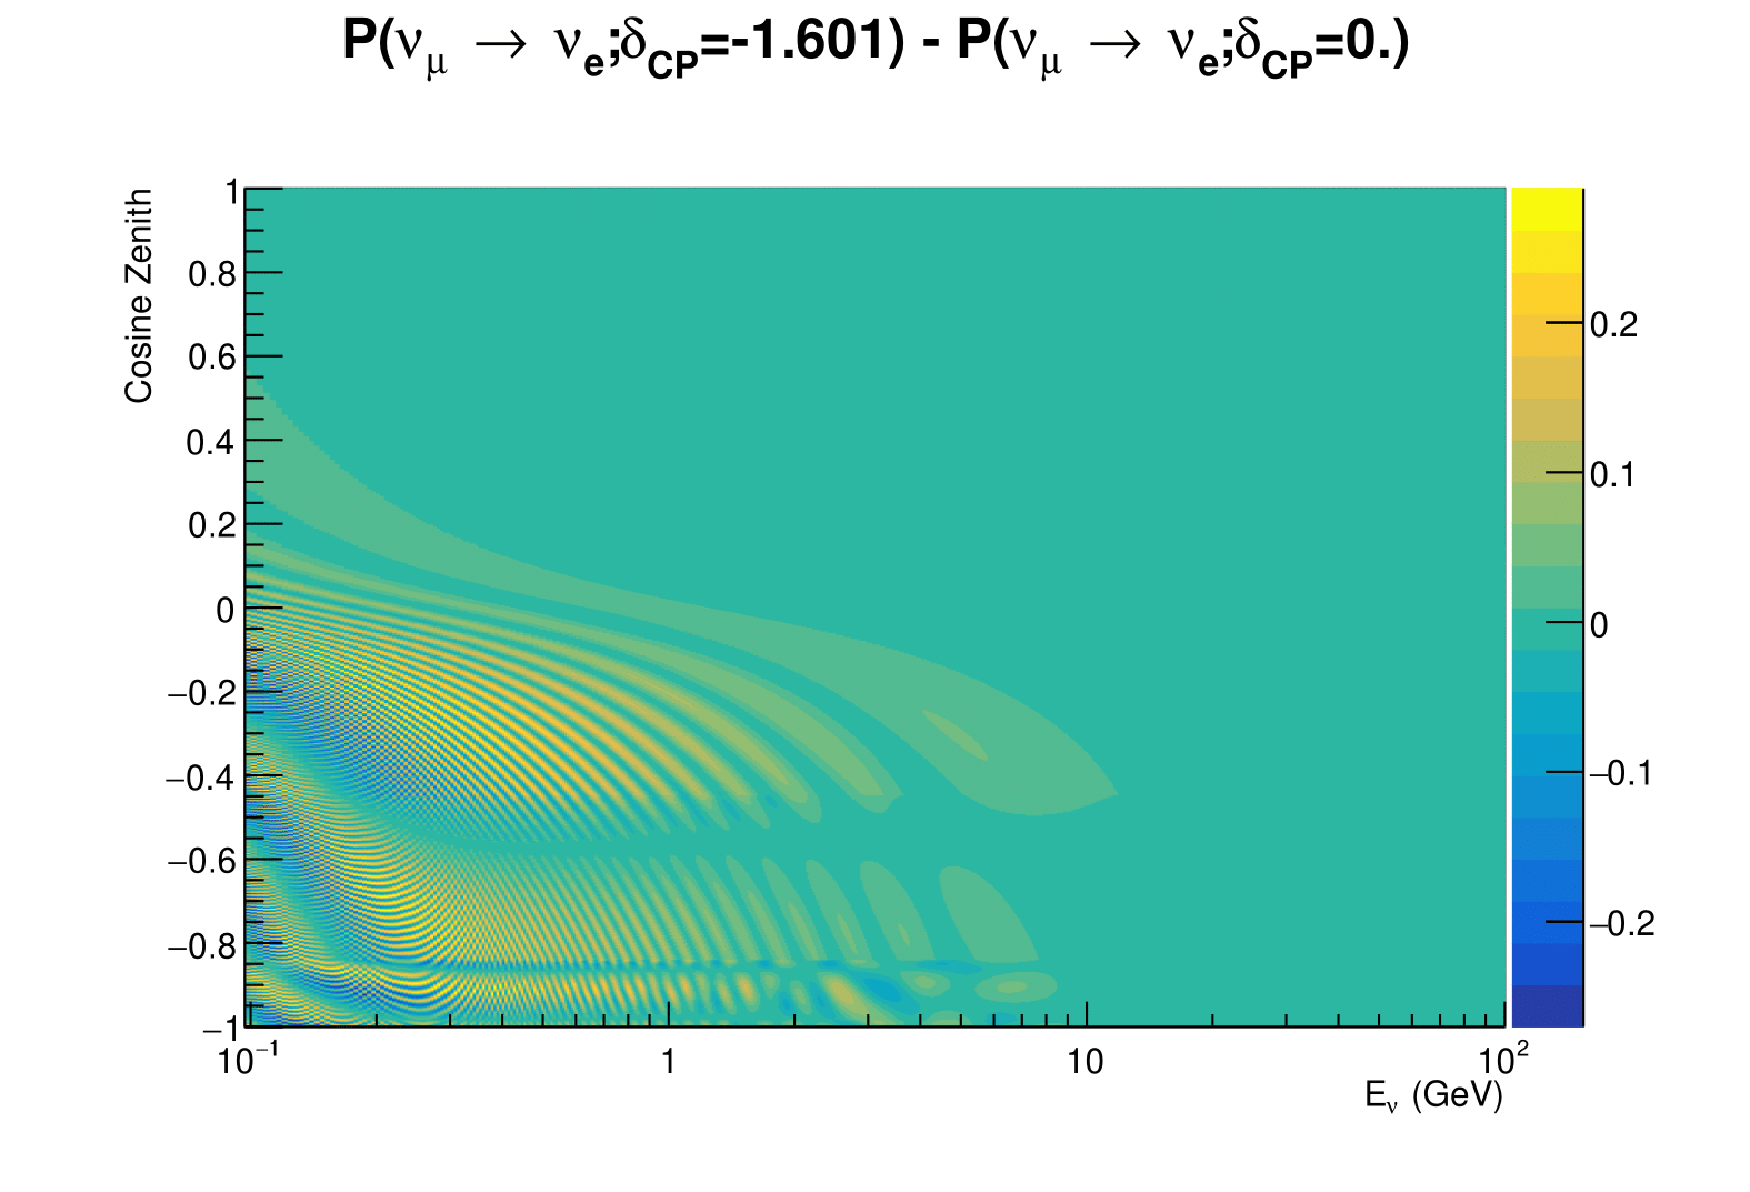
\includegraphics[width=\textwidth, trim={0mm 0mm 0mm 0mm}, clip,page=1]{Figures/Oscillation/AtmDCPSens.pdf}
  \end{subfigure}
  \caption{The effect of \quickmath{\delta_{CP}} for atmospheric neutrinos given in terms of the neutrino energy and zenith angle. This oscillogram compares the \quickmath{P(\nu_{\mu} \rightarrow \nu_{e})} oscillation probability for a CP conserving (\quickmath{\delta_{CP}=0.0}) and a CP violating (\quickmath{\delta_{CP}=-1.601}) value taken from the Asimov A parameter set. The other oscillation parameters assume the Asimov A oscillation parameter set given in \autoref{tab:Theory_ParameterSets}.}
  \label{fig:Oscillation_SK_DCPSensitivity}
\end{figure}

The vacuum and matter oscillation probabilities for \quickmath{P(\nu_{e} \rightarrow \nu_{e})} and \quickmath{P(\bar{\nu}_{e} \rightarrow \bar{\nu}_{e})} are presented in \autoref{fig:Oscillation_SK_VacuumMatter}, where the PREM model has been assumed. The oscillation probability for both neutrinos and antineutrinos is affected in the presence of matter. However, the resonance effects around \quickmath{O(5)\text{GeV}} only occur for neutrinos in the normal mass hierarchy and antineutrinos in the inverse mass hierarchy. The exact position and amplitude of the resonance depend on \quickmath{\sin^{2}(\theta_{23})}, further increasing the atmospheric neutrinos' sensitivity to the parameter.

\begin{figure}[h]
  \begin{subfigure}[t]{\textwidth}
    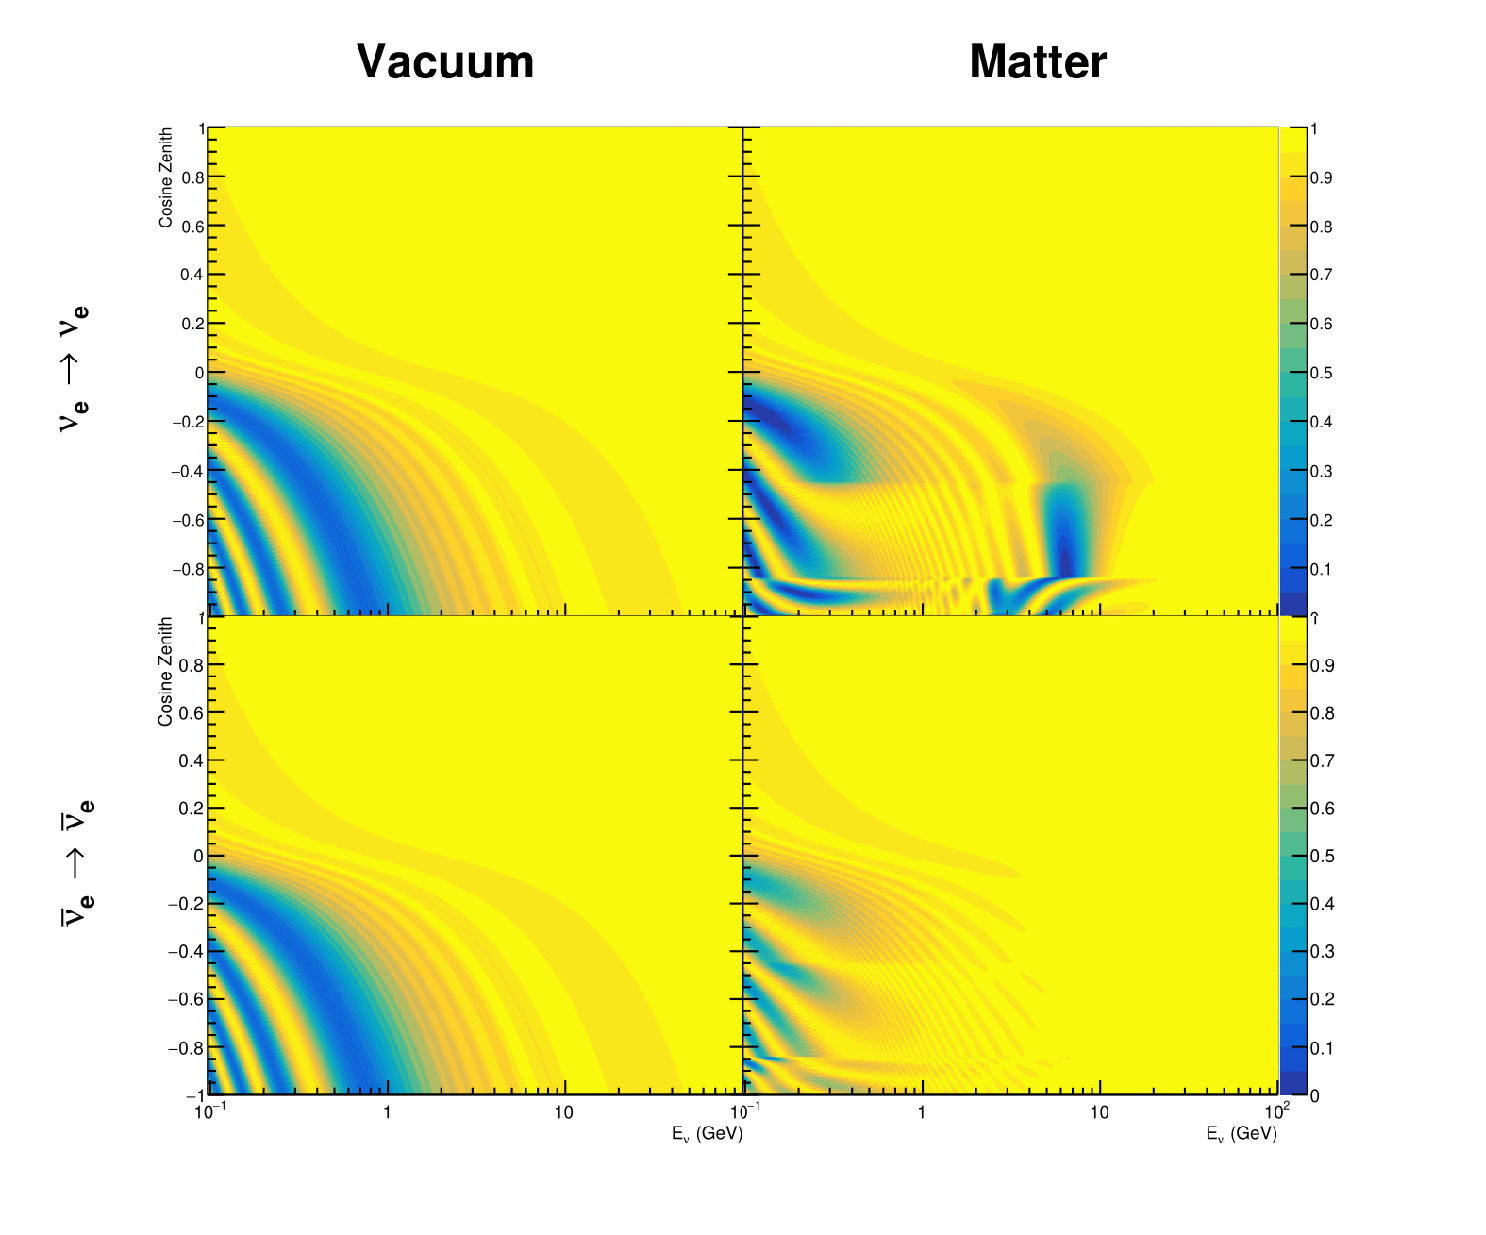
\includegraphics[width=\textwidth, trim={0mm 0mm 0mm 0mm}, clip,page=1]{Figures/Oscillation/MatterEffect.pdf}
  \end{subfigure}
  \caption{An illustration of the matter-induced effects on the oscillation probability, given as a function of neutrino energy and zenith angle. The top row of panels gives the \quickmath{P(\nu_{e} \rightarrow \nu_{e})} oscillation probability and the bottom row illustrates the \quickmath{P(\bar{\nu}_{e} \rightarrow \bar{\nu}_{e})} oscillation probability. The left column highlights the oscillation probability in a vacuum, whereas the middle and right column represents the oscillation probabilities when the four-layer fixed density PREM model is assumed. All oscillation probabilities assume the ``Asimov A'' set given in \autoref{tab:Theory_ParameterSets}, but importantly, the right column sets an inverted mass hierarchy. The ``matter resonance'' effects at \quickmath{E_{\nu} \sim 5\text{GeV}} can be seen in the \quickmath{P(\nu_{e} \rightarrow \nu_{e})} for normal mass hierarchy and \quickmath{P(\bar{\nu}_{e} \rightarrow \bar{\nu}_{e})} for inverted hierarchy.}
  \label{fig:Oscillation_SK_VacuumMatter}
\end{figure}

As the T2K beam flux is centered at the first oscillation maximum (\quickmath{E_{\nu} = 0.6\text{GeV}}) \cite{t2k_det}, the sensitivity to \quickmath{\delta_{CP}} is predominantly observed as a change in the event-rate of e-like samples in \quickmath{\nu/\bar{\nu}} modes. \autoref{fig:Oscillation_T2K_OscillationProbSensitivity} illustrates the \quickmath{P(\nu_\mu \rightarrow \nu_e)} oscillation probability for a range of \quickmath{\delta_{CP}} values. %The magnitude of the oscillation peak has an approximate factor of two difference between the CP-violating values \quickmath{\delta_{CP} = \pm\pi/2} and the difference in oscillation probability between the CP-conserving
A circular modulation of the first oscillation peak (in both magnitude and position) is observed when varying throughout the allowable values of \quickmath{\delta_{CP}}. The CP-conserving values of \quickmath{\delta_{CP}=0,\pi} have a lower(higher) oscillation maximum than the CP-violating values of \quickmath{\delta_{CP}=-\pi/2}(\quickmath{\delta_{CP}=\pi/2}). A sub-dominant shift in the energy of the oscillation peak is also present, which aids in separating the two CP-conserving values of \quickmath{\delta_{CP}}.

\begin{figure}[h]
  \begin{subfigure}[t]{0.5\textwidth}
    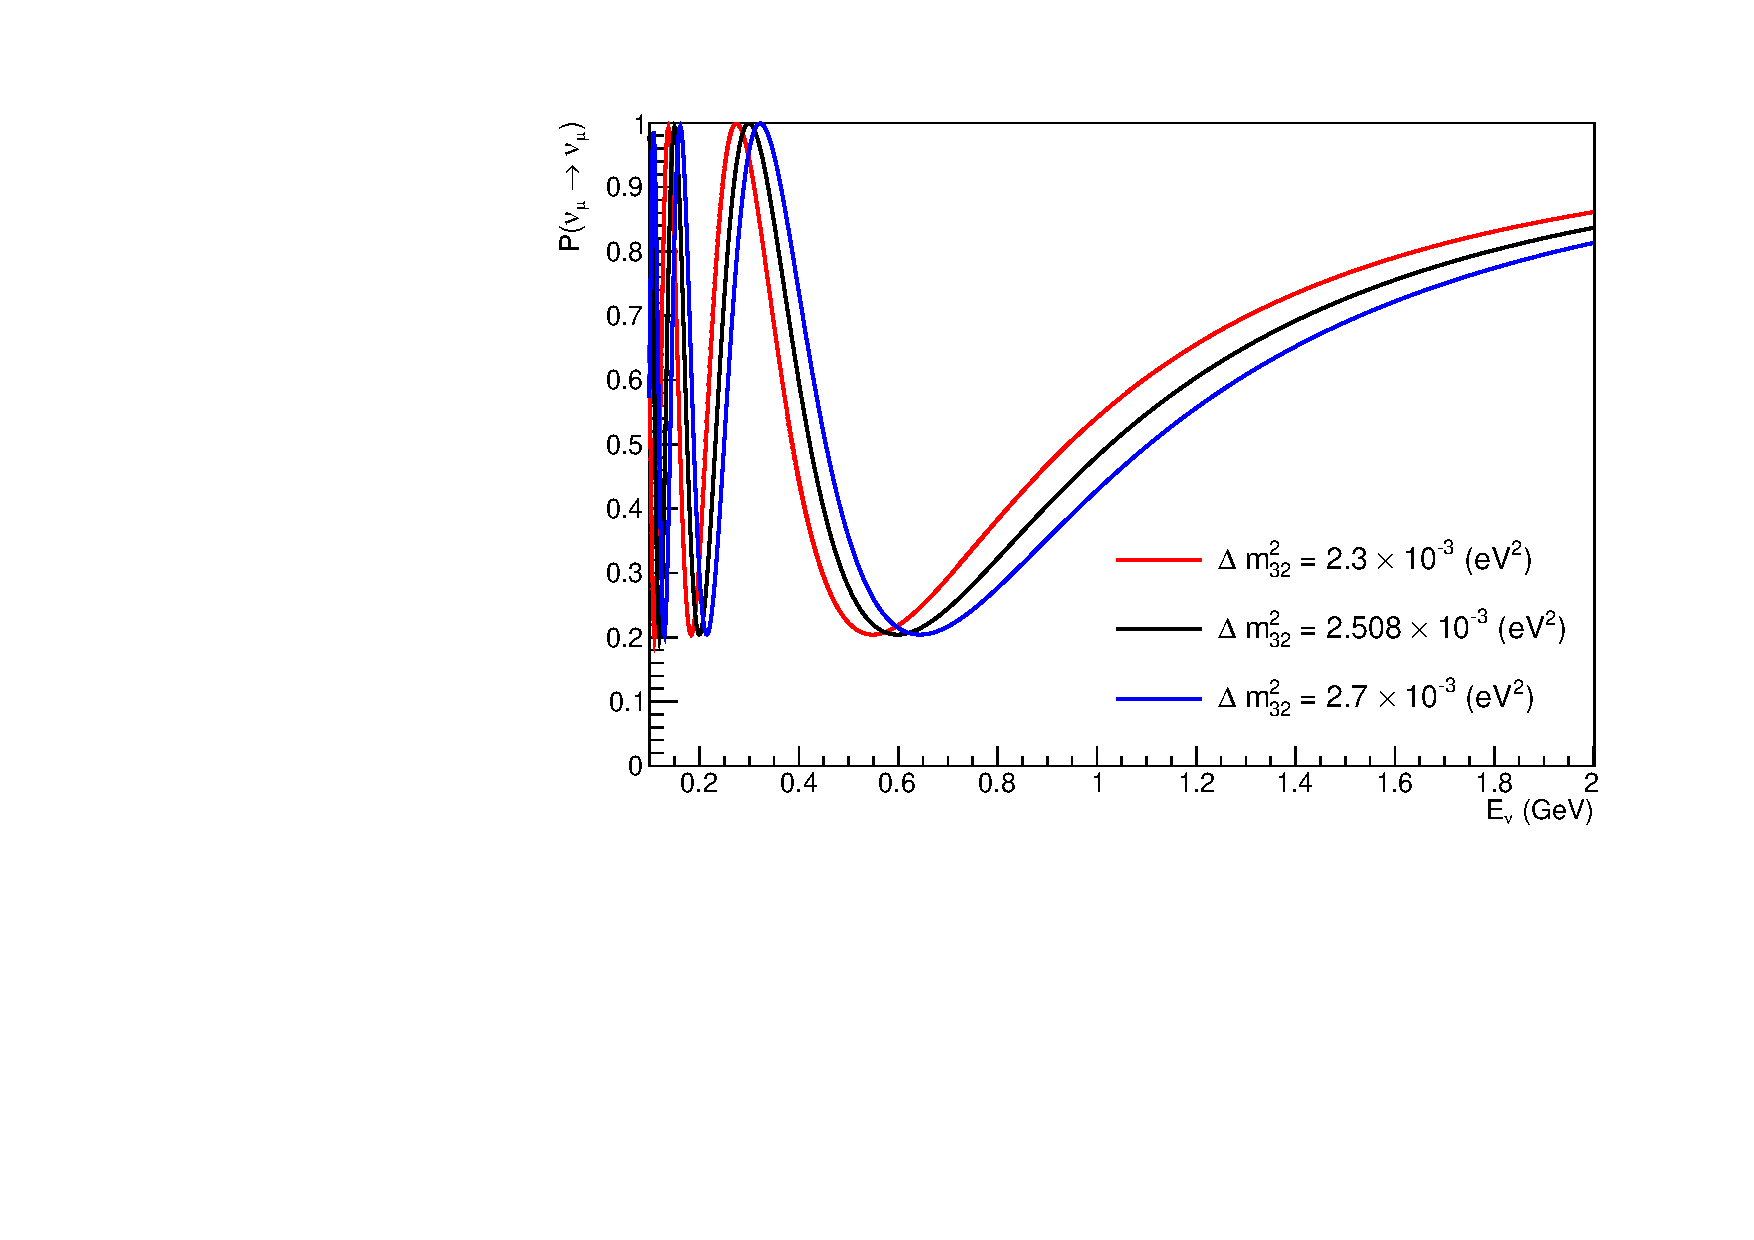
\includegraphics[width=\textwidth, trim={0mm 0mm 0mm 0mm}, clip,page=1]{Figures/Oscillation/T2K_NuMu_x_NuMu_DelMsq32Sens.pdf}
    \subcaption{\quickmath{\Delta m^{2}_{32}}}
  \end{subfigure}%
  \begin{subfigure}[t]{0.5\textwidth}
    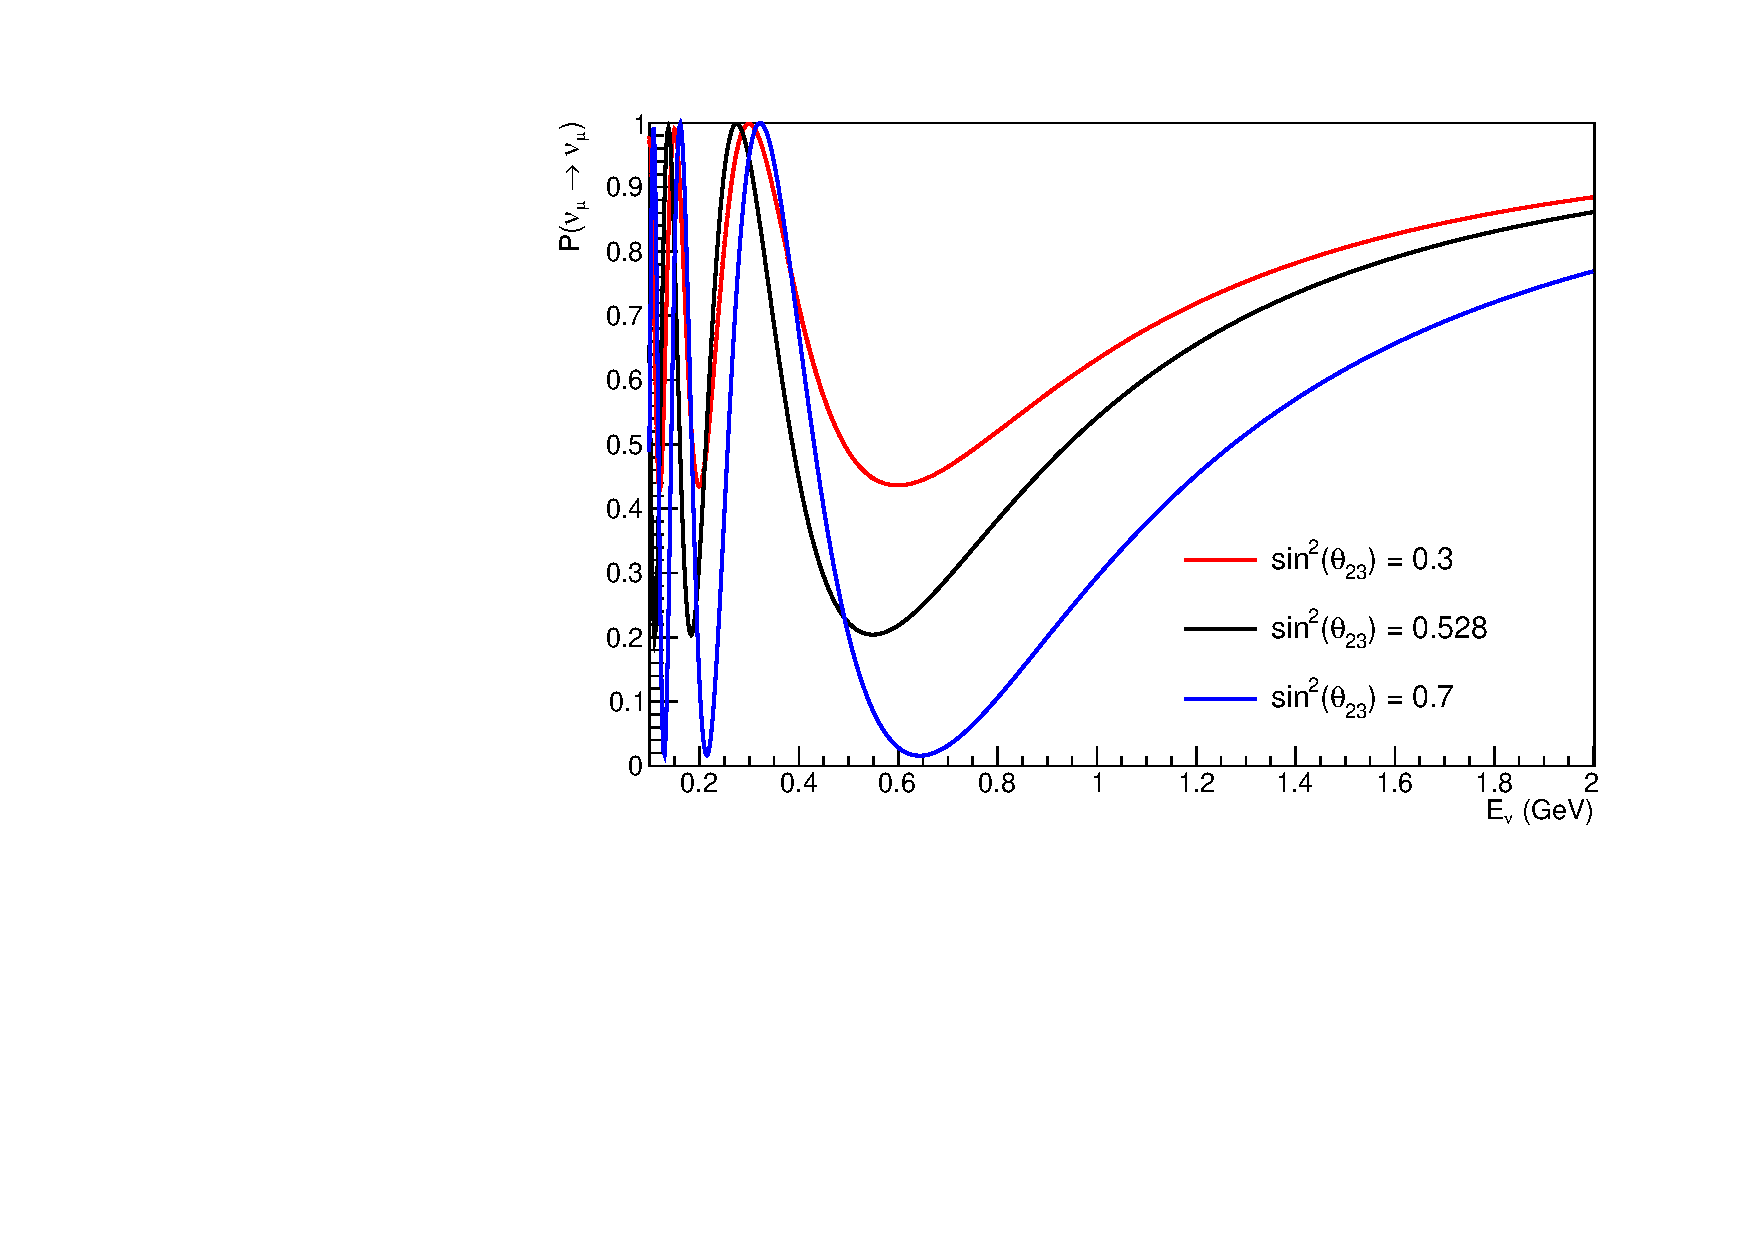
\includegraphics[width=\textwidth, trim={0mm 0mm 0mm 0mm}, clip,page=1]{Figures/Oscillation/T2K_NuMu_x_NuMu_Sinsqth23Sens.pdf}
    \subcaption{\quickmath{\sin^{2}(\theta_{23})}}
  \end{subfigure}
  \begin{subfigure}[t]{0.5\textwidth}
    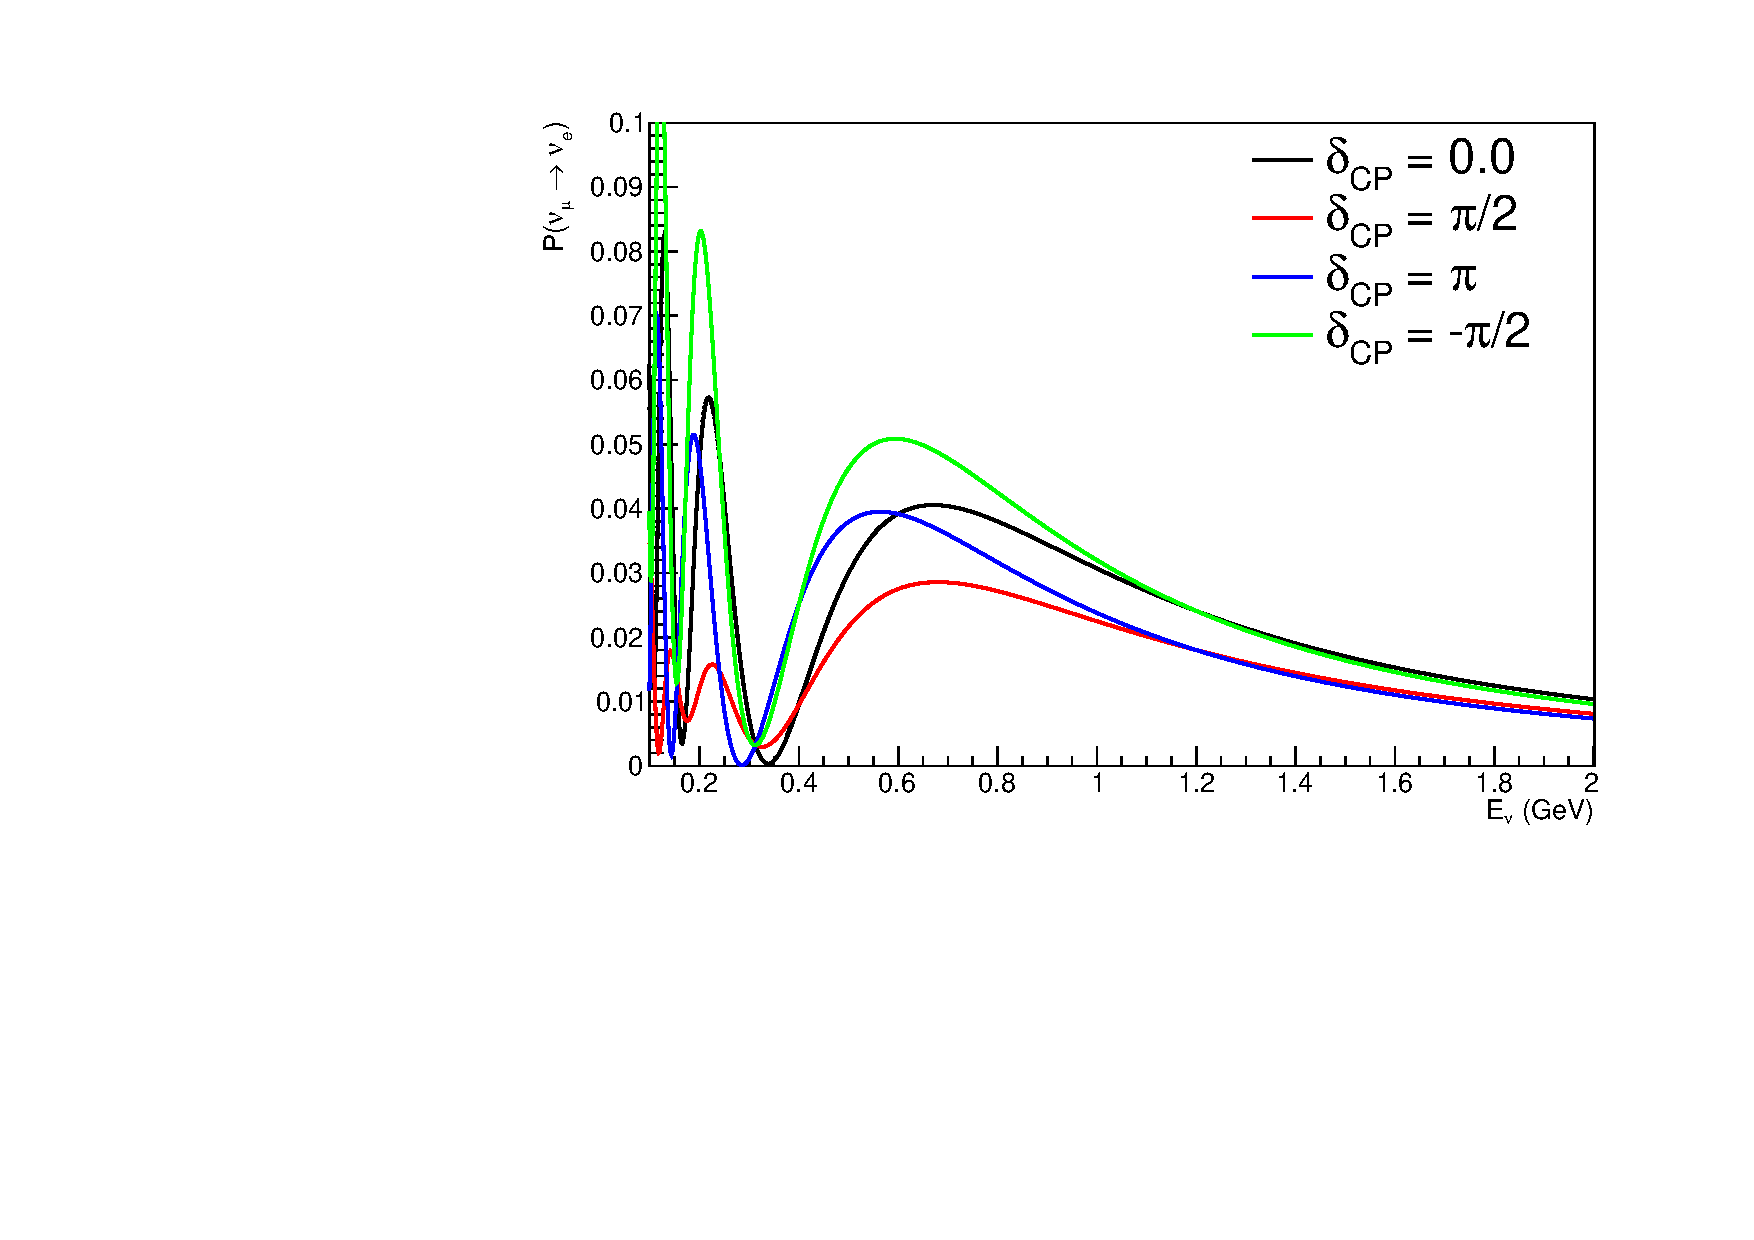
\includegraphics[width=\textwidth, trim={0mm 0mm 0mm 0mm}, clip,page=1]{Figures/Oscillation/T2K_NuMu_x_NuE_DCPSens.pdf}
    \subcaption{\quickmath{\delta_{CP}}}
  \end{subfigure}
  \caption{The oscillation probability for beam neutrino events given as a function of neutrino energy. All oscillation parameters assume the ``Asimov A'' set given in \autoref{tab:Theory_ParameterSets} unless otherwise stated. A path-length of \quickmath{295\text{km}} is assumed. Each panel represents a change in one of the oscillation parameters whilst keeping the remaining parameters fixed.}
  \label{fig:Oscillation_T2K_OscillationProbSensitivity}
\end{figure}

\newpage

T2K's sensitivity to \quickmath{\sin^{2}(\theta_{23})} and \quickmath{\Delta m^{2}_{32}} is observed as a shape-based variation of the muon-like samples, as illustrated in \autoref{fig:Oscillation_T2K_OscillationProbSensitivity}. The value of \quickmath{\Delta m^{2}_{32}} laterally shifts the position of the oscillation dip (around \quickmath{E_\nu \sim 0.6\text{GeV}}) in the \quickmath{P(\nu_\mu \rightarrow \nu_\mu)}. A variation of \quickmath{\sin^{2}(\theta_{23})} is predominantly observed as a vertical shift of the oscillation dip with second-order horizontal shifts being due to matter effects. The beam neutrinos have limited sensitivity to matter effects due to the relatively shorter baseline as well as the Earth's mantle being a relatively low-density material (as compared to the Earth's core). For some values of \quickmath{\delta_{CP}}, the degeneracy in the number of e-like events allows the mass hierarchy to be broken. This leads to a \quickmath{\delta_{CP}}-dependent mass hierarchy sensitivity which can be seen in \autoref{fig:Oscillation_SK_BiProbabilityPlot}.

\begin{figure}[h]
  \begin{subfigure}[t]{0.65\textwidth}
    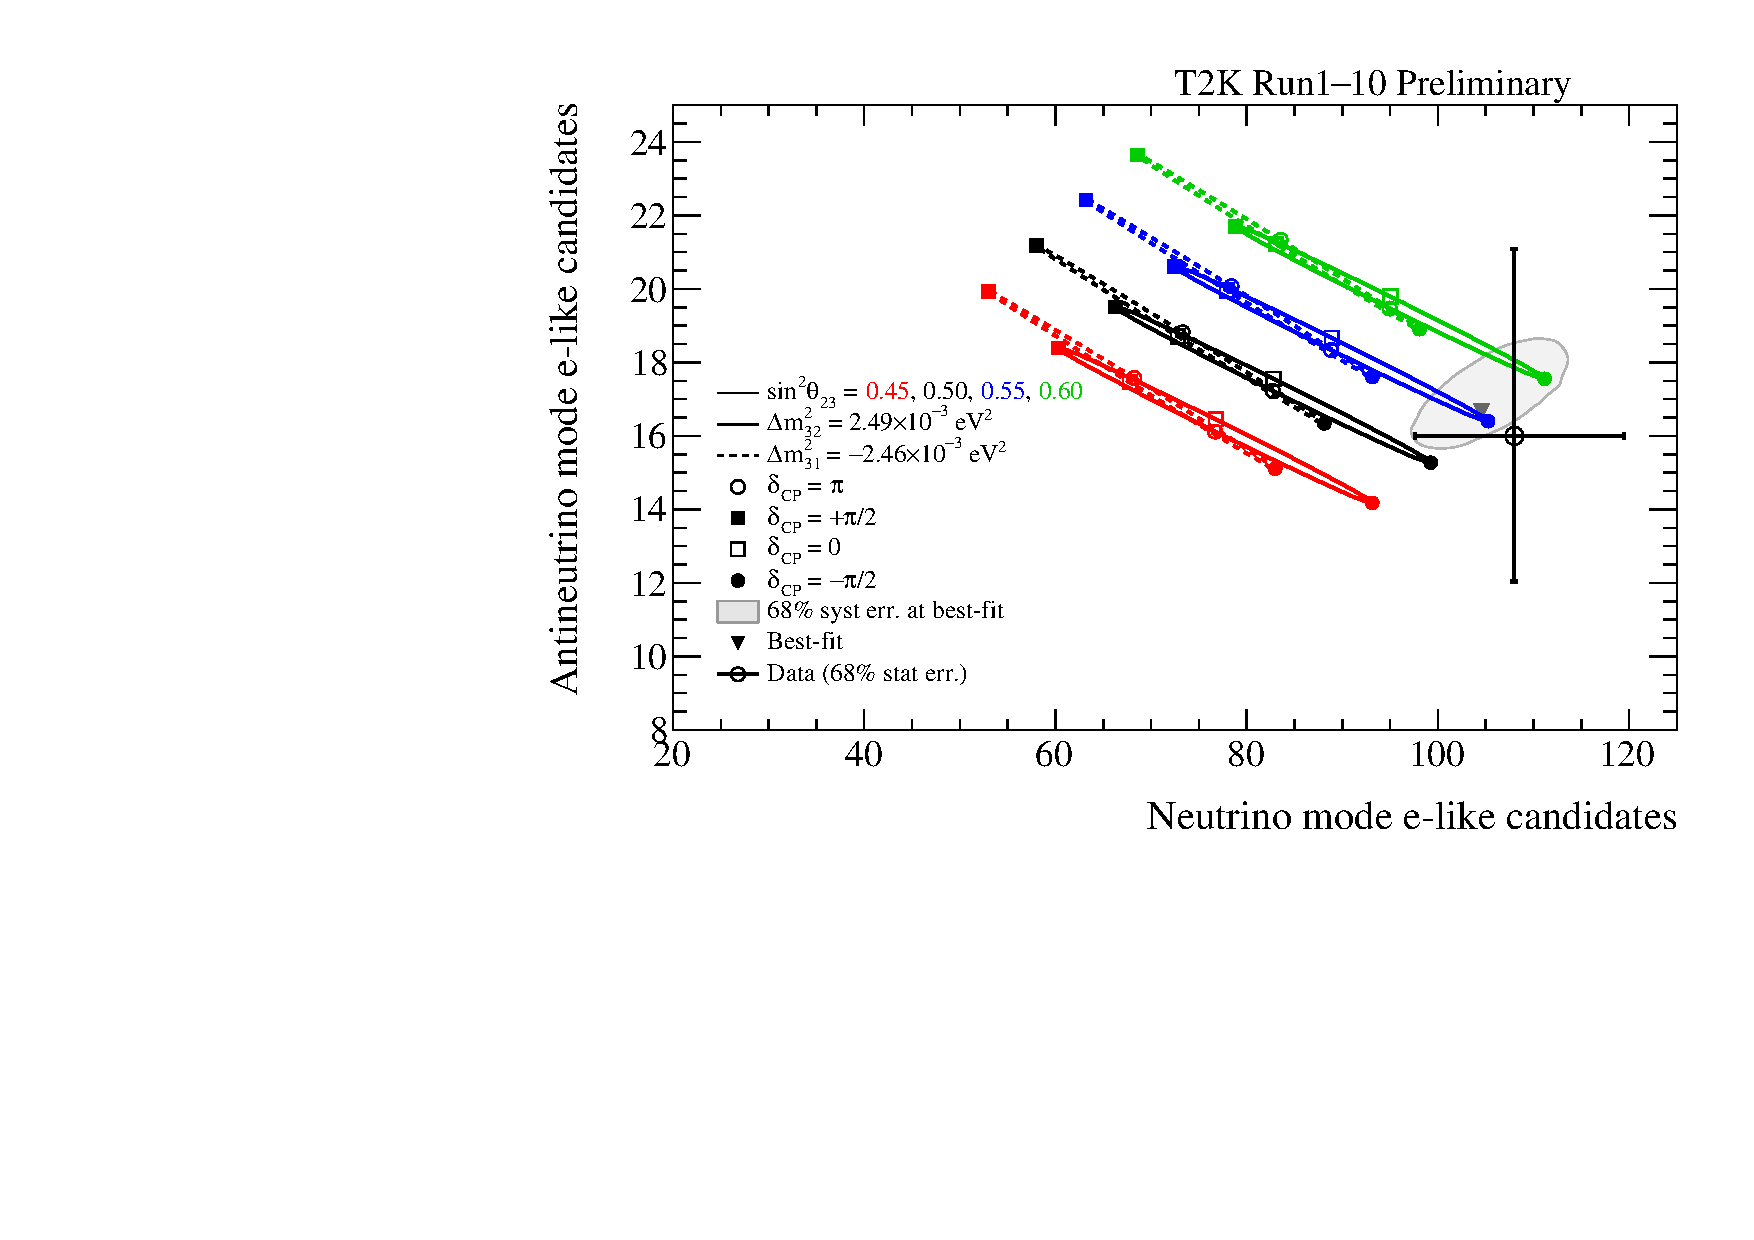
\includegraphics[width=\textwidth, trim={0mm 0mm 0mm 0mm}, clip,page=1]{Figures/Oscillation/BiProbabilityPlot.pdf}
  \end{subfigure}
  \caption{The number of electron-like events in the FHC and RHC operating mode of the beam, as a function of the oscillation probabilities. Both normal hierarchy (Solid)) and inverse hierarchy (Dashed) values of \quickmath{\Delta m^{2}_{32}} are given.}
  \label{fig:Oscillation_SK_BiProbabilityPlot}
\end{figure}

Whilst all oscillation channels should be included for completeness, the computational resources required to run a fit are limited and any reasonable approximations which reduce the number of oscillation probability calculations that need to be made should be applied. The \quickmath{\nu_{e} \rightarrow \nu_{e,\mu,\tau}} (and antineutrino equivalent) oscillations can be ignored for beam neutrinos as the \quickmath{\nu_{e}/\bar{\nu}_{e}} fluxes are approximately two orders of magnitude smaller than the corresponding \quickmath{\nu_{\mu}/\bar{\nu}_{\mu}} flux \cite{Abe2021-tr}. Furthermore, as the peak neutrino energy of the beam is well below the threshold for charged current tau production (\quickmath{E_\nu = 3.5\text{GeV}} \cite{Li_2018}), only a small proportion of the neutrinos produced in the beam have the required energy. For the few neutrinos that have sufficient energy, the oscillation probability is very small due to their energy being well above the oscillation maximum (small value of \quickmath{L/E}). Whilst these approximations have be made for the beam neutrinos, the atmospheric flux of \quickmath{\nu_{e}} is of the same order of magnitude as the \quickmath{\nu_{\mu}} flux and the energy distribution of atmospheric neutrinos extends well above the tau production threshold. These events can have non-negligible oscillation probabilities due to the further distance they travel.

\chapter{T2K and SK Experiment Overview}
\label{chap:T2KSKExp}

As the successor of the Kamiokande experiment, the Super-Kamiokande (SK) collaboration has been leading atmospheric neutrino oscillation analyses for over two decades. The detector has provided some of the strongest constraints on proton decay and the first precise measurements of the \delmsqatm and \sinsqatm neutrino oscillation parameters.
%The ability of the detector to observe low-energy neutrino events has been significantly improved with the recent gadolinium doping of the ultra-pure water target.
The history, detection technique, and operation of the SK detector is described in \autoref{sec:T2KSKExp_SK}.

The Tokai-to-Kamioka (T2K) experiment was one of the first long-baseline experiments to use both neutrino and antineutrino beams to precisely measure the charge parity violation within the neutrino sector. The T2K experiment observed the first hints of a non-zero \sinsqreac measurement and continues to lead the field with the constraints it provides on \sinsqreac, \sinsqatm, \delmsqatm and \dcp.
In \autoref{sec:T2KSKExp_T2K}, the techniques that T2K use to generate the neutrino beam and constrain systematic parameter through near detector constraints are described.

%The techniques which T2K uses in generating its neutrino beam as well as the near-detector used to constrain the flux and cross-section parameters used in this analysis are documented in \autoref{sec:T2KSKExp_T2K}.

\section{The Super-Kamiokande Experiment}
\label{sec:T2KSKExp_SK}

The SK experiment began taking data in 1996 \cite{Fukuda1998-tw} and has had many modifications throughout its operation. There have been seven defined periods of data taking as noted in \autoref{tab:T2KSKExp_SKPeriods}. Data taking began in SK-I which ran for five years. Between the SK-I and SK-II periods, approximately \quickmath{55\%} of the PMTs were damaged during maintenance \cite{Abe_2014_SKCalib}. Those that survived were equally distributed throughout the detector in the SK-II era, which resulted in a reduced \quickmath{19\%} photo-coverage. From SK-III onwards, repairs to the detector meant the full suite of PMTs was operational recovering the \quickmath{40\%} photocoverage. Before the start of SK-IV, the data acquisition and electronic systems were upgraded. Between SK-IV and SK-V, a significant effort was placed into tank open maintenance and repair/replacement of defective PMTs, a task for which the author of this thesis was required. Consequently, the detector conditions were significantly different between the two operational periods. SK-VI marked the start of the SK-Gd era, with the detector being doped with gadolinium at a concentration of \quickmath{0.01\%}. SK-VII, which started during the writing of this thesis, has increased the gadolinium concentration to \quickmath{0.03\%} for continued operation \cite{10.5281/zenodo.6694761}.

The oscillation analysis presented within this thesis focuses on the SK-IV period of running and the data taking within it. This follows from the recent SK analysis presented in \cite{thesis_miao}. Therefore, the information presented within this section focuses on that period.

\begin{table}[ht!]
    \centering
    \begin{tabular}{c|l|l|c}
      \hline
      Period & Start Date & End Date & Live-time (days) \\
      \hline
      I & April 1996 & July 2001 & 1489.19 \\
      II & October 2002 & October 2005 & 798.59 \\
      III & July 2006 & September 2008 & 518.08 \\
      IV & September 2008 & May 2018 & 3244.4 \\
      V & January 2019 & July 2020 & 461.02 \\
      VI & July 2020 & May 2022 & 583.3 \\
      VII & May 2022 & Ongoing & N/A \\
      \hline 
      \hline
    \end{tabular}
    \caption{The various SK periods and respective live-time. The SK-VI live-time is calculated until \quickmath{1^{\text{st}}} April 2022. SK-VII started during the writing of this thesis.}
    \label{tab:T2KSKExp_SKPeriods}
\end{table}

\subsection{The SK Detector}
\label{subsec:T2KSKExp_SKDetector}

The basic structure of the Super-Kamiokande (SK) detector is a cylindrical tank with a diameter \quickmath{39.3\text{m}} and height \quickmath{41.1\text{m}} filled with ultrapure water \cite{Abe_2014_SKCalib}. A diagram of the significant components of the SK detector is given in \autoref{fig:T2KSKExp_SK_Diag}. The SK detector is situated in the Kamioka mine in Gifu, Japan. The mine is underground with roughly \quickmath{1\text{km}} rock overburden (\quickmath{2.7 \text{km}} water equivalent overburden) \cite{Fukuda2003-ly}. At this depth, the rate of cosmic ray muons is significantly decreased to a value of \quickmath{\sim 2\text{Hz}}. The top of the tank is covered with stainless steel which is designed as a working platform for maintenance, calibration, and location for high voltage and data acquisition electronics.

\begin{figure}[h]
  \begin{subfigure}[t]{0.95\textwidth}
    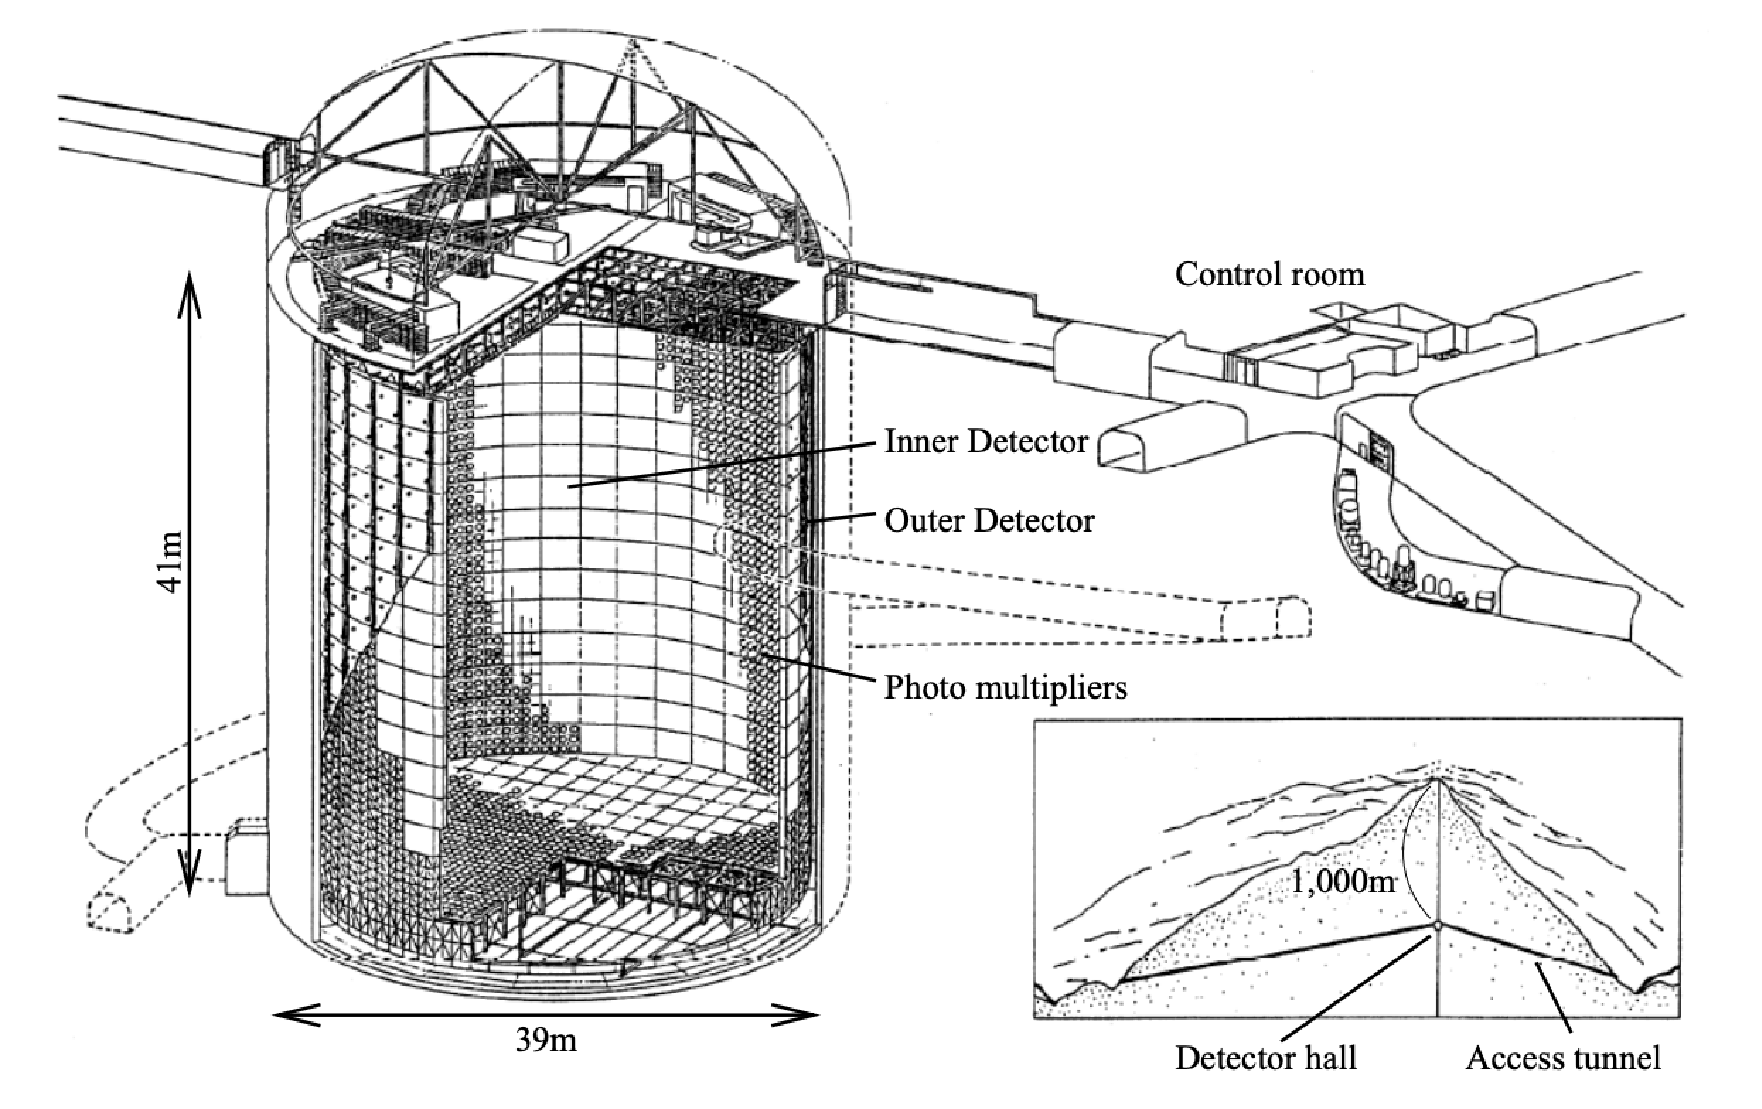
\includegraphics[width=\textwidth, trim={0mm 0mm 0mm 0mm}, clip,page=1]{Figures/Detectors/SKDiagram.pdf}
  \end{subfigure}
  \caption{A schematic diagram of the Super-Kamiokande Detector. Taken from \cite{Itow2001-bc}.}
  \label{fig:T2KSKExp_SK_Diag}
\end{figure}

A smaller cylindrical structure (\quickmath{36.2\text{m}} diameter, \quickmath{33.8\text{m}} height) is situated inside the tank, with an approximate \quickmath{2\text{m}} gap between this structure and the outer tank wall. The purpose of this structure is to support the photomultiplier tubes (PMTs). The volume inside and outside the support structure is referred to as the inner detector (ID) and outer detector (OD), respectively. In the SK-IV era, the ID and OD are instrumented by \quickmath{11,129} \quickmath{50\text{cm}} and \quickmath{1,885} \quickmath{20 \text{cm}} PMTs respectively \cite{Abe_2014_SKCalib}. The ID contains a \quickmath{32\text{kton}} mass of water. Many analyses performed at SK use a ``fiducial volume'' defined by the volume of water inside the ID excluding some distance to the ID wall. This reduces the volume of the detector which is sensitive to neutrino events but reduces radioactive backgrounds and allows for better reconstruction performance. The nominal fiducial volume is defined as the area contained inside \quickmath{2\text{m}} from the ID wall for a total of \quickmath{22.5\text{kton}} water \cite{Jiang2019-iw}.

The two regions of the detector (ID and OD) are optically separated with opaque black plastic hung from the support structure. The purpose of this is to determine whether an event entered or exited the ID. This allows cosmic ray muons and partially contained events to be tagged and separated from neutrino events entirely contained within the ID. This black plastic is also used to cover the area between the ID PMTs to reduce photon reflection from the ID walls. Opposite to this, the OD is lined with a reflective material to allow photons to reflect around inside the OD until collected by one of the PMTs. Furthermore, each OD PMT is optically coupled with \quickmath{50\times50\text{cm}} plates of wavelength shifting acrylic which increases the efficiency of light collection \cite{Fukuda2003-ly}.

In the SK-IV data-taking period, the photocathode coverage of the detector, or the fraction of the ID wall instrumented with PMTs, is \quickmath{\sim 40\%} \cite{Fukuda2003-ly}. The PMTs have a quantum efficiency (the ratio of detected electrons to incident photons) of \quickmath{\sim 21\%} for photons with wavelengths of \quickmath{360\text{nm} < \lambda < 390\text{nm}} \cite{Suzuki1993}. The proportion of photoelectrons that produce a signal in the dynode of a PMT, termed the collection efficiency, is \quickmath{>70 \%} \cite{Fukuda2003-ly}. The PMTs used within SK are most sensitive to photons with wavelength \quickmath{300\text{nm} \leq \lambda \leq 600\text{nm}} \cite{Fukuda2003-ly}. One disadvantage of using PMTs as the detection media is that the Earth's geomagnetic field can modify its response. Therefore, a set of compensation coils is built around the inner surface of the detector to mitigate this effect \cite{t2k_sk}.

As mentioned, the SK detector is filled with ultrapure water, which in a perfect world would contain no impurities. However, bacteria and organic compounds can significantly degrade the water quality. This decreases the attenuation length, which reduces the total number of photons that hit a PMT. To combat this, a sophisticated water treatment system has been developed \cite{Fukuda2003-ly, Nakano2020-sb}. UV lights, mechanical filters, and membrane degasifiers are used to reduce the bacteria, suspended particulates, and radioactive materials from the water. The flow of water within the tank is also critical as it can remove stagnant bacterial growth or build-up of dust on the surfaces within the tank. Gravity drifts impurities in the water towards the bottom of the tank which, if left uncontrolled, can create asymmetric water conditions between the top and bottom of the tank.
%The flow of water in the tank can be controlled via mechanically driven circulation or temperature driven convection.
Typically, the water entering the tank is cooled below the ambient temperature of the tank to control convection and inhibit bacteria growth. Furthermore, the rate of dark noise hits within PMTs is sensitive to the PMT temperature \cite{HamamatsuPMT} so controlling the temperature gradients within the tank is beneficial for stable measurements.

SK-VI is the first phase of the SK experiment to use gadolinium dopants within the ultrapure water \cite{10.5281/zenodo.6694761}. As such, the SK water system had to be replaced to avoid removing the gadolinium concentrate from the ultrapure water \cite{Abe2022-qq}. For an inverse \quickmath{\beta}-decay (IBD) interaction in a water target, the emitted neutron is thermally captured on hydrogen. This process releases \quickmath{2.2 \text{MeV}} \quickmath{\gamma} ray which are difficult to detect as the resulting Compton scattered electrons are very close to the Cherenkov threshold, limiting detection capability. Thermal capture of neutrons on gadolinium generates \quickmath{\gamma} rays with higher energy (\quickmath{8\text{MeV}} \cite{Abe2022-ij}) meaning they are more easily detected and reconstructed. SK-VI has \quickmath{0.01 \%} Gd loading (\quickmath{0.02\%} gadolinium sulphate by mass) which causes \quickmath{\approx 50\%} of neutrons emitted by IBD to be captured on gadolinium\cite{PhysRevLett.93.171101,Marti2020-le} . Whilst predominantly useful for low energy analyses, Gd loading allows better \quickmath{\nu/\bar{\nu}} separation for atmospheric neutrino event selections \cite{Marti2019-gu}. Efforts are currently in place to increase the gadolinium concentrate to \quickmath{0.03 \%} for \quickmath{\approx 75\%} neutron capture efficiency on gadolinium \cite{Vagins2022-sj}. The final stage of loading targets \quickmath{0.1 \%} concentrate targeting \quickmath{\approx 90\%} neutron capture efficiency on gadolinium.

\subsection{Calibration}
\label{subsec:T2KSKExp_SKCalibration}

The calibration of the SK detector is documented in \cite{Abe_2014_SKCalib} and summarised below. The analysis presented within this thesis is dependent upon `high energy events' (Charged particles with \quickmath{O(>100)\text{MeV}} momenta). These are events that are expected to generate a larger number of photons such that each PMT will be hit with multiple photons. The reconstruction of these events depends upon the charge deposited within each PMT and the timing response of each individual PMT. Therefore, the most relevant calibration techniques to this thesis are outlined.

Before installation, \quickmath{420} PMTs were calibrated to have identical charge responses and then distributed throughout the tank in a cross-shape pattern (As illustrated by \autoref{fig:T2KSKExp_SK_StandardPMTs}). These are used as a standardised measure for the rest of the PMTs installed at similar geometric positions within SK to be calibrated against.
%This allows each PMT to have it's high voltage set so that all PMTs give the same signal for an identical light collection.
To perform this calibration, a xenon lamp is located at the centre of the SK tank which flashes uniform light at \quickmath{1 \text{Hz}}. This allows for geometrical effects, water quality variation, and timing effects to be measured in-situ throughout normal data-taking periods.

\begin{figure}[h]
  \begin{subfigure}[t]{0.50\textwidth}
    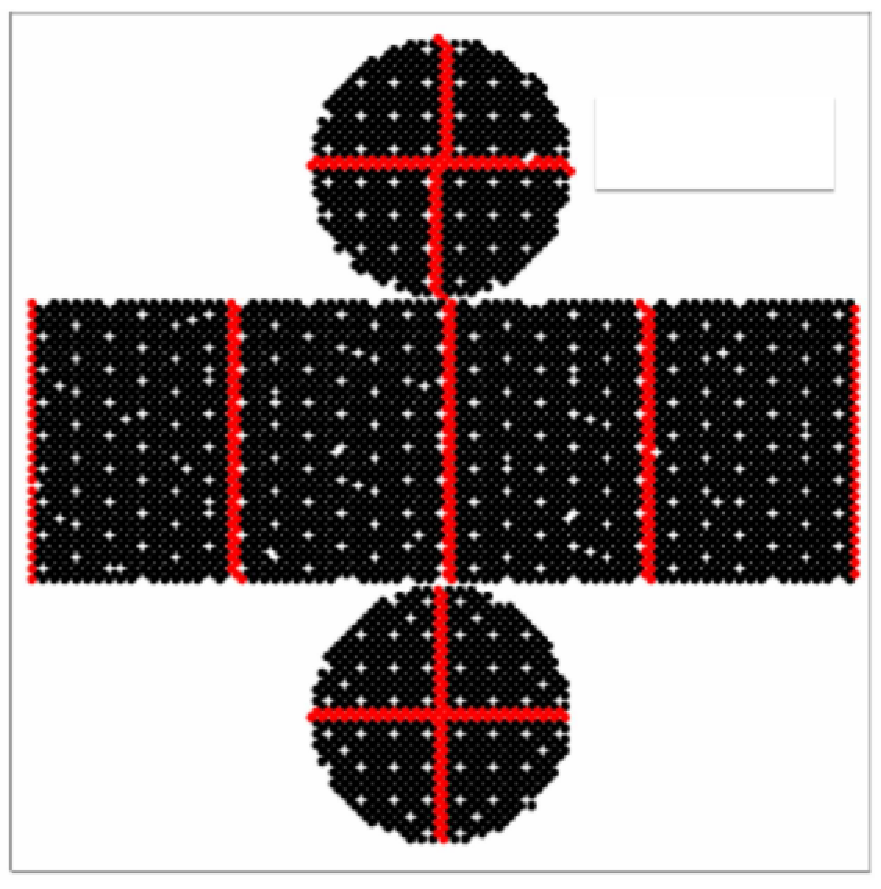
\includegraphics[width=\textwidth, trim={0mm 0mm 0mm 0mm}, clip,page=1]{Figures/Detectors/StandardPMTs.pdf}
  \end{subfigure}
  \caption{The location of ``standard PMTs'' (red) inside the SK detector. Taken from \cite{Abe_2014_SKCalib}.}
  \label{fig:T2KSKExp_SK_StandardPMTs}
\end{figure}

When specifically performing calibration of the detector (in out-of-data taking mode), the water in the tank was circulated to avoid top/bottom asymmetric water quality. Any non-uniformity within the tank significantly affects the PMT hit probability through scattering or absorption. This becomes a dominant effect for the very low-intensity light sources discussed later which are designed such that only one photon is incident upon a given PMT.

The ``gain'' of a PMT is defined as the ratio of the total charge of the signal produced compared to the charge of photoelectrons emitted by the photocathodes within the PMT. To calibrate the signal of each PMT, the ``relative'' and ``absolute'' gain values are measured. The relative gain is the variation of gain among each of the PMTs whereas the absolute gain is the average gain of all PMTs. 

The relative gain is calibrated as follows. A laser is used to generate two measurements: a high-intensity flash that illuminates every PMT with a sufficient number of photons, and a low-intensity flash in which only a small number of PMTs collect light. The first measurement creates an average charge, \quickmath{Q_{obs}(i)} on PMT \quickmath{i}, whereas the second measurement ensures that each hit PMT only generates a single photoelectron. For the low-intensity measurement, the number of times each PMT records a charge larger than \quickmath{1/4} photoelectrons, \quickmath{N_{obs}(i)}, is counted. The values measured can be expressed as

\begin{equation}
  \label{eq:T2KSKExp_RelativeGainCalib}
  \begin{split}
    Q_{obs}(i) &\propto I_{H} \times f(i) \times \epsilon(i) \times G(i), \\
    N_{obs}(i) &\propto I_{L} \times f(i) \times \epsilon(i),
  \end{split}
\end{equation}

Where \quickmath{I_{H}} and \quickmath{I_{L}} is the intensity of the high and low flashes, \quickmath{f(i)} is the acceptance efficiency of the \quickmath{i^{\text{th}}} PMT, \quickmath{\epsilon(i)} is the product of the quantum and collection efficiency of the \quickmath{i^{\text{th}}} PMT and \quickmath{G(i)} is the gain of the \quickmath{i^{\text{th}}}	PMT. The relative gain for each PMT can determined by taking the ratio of these quantities.

The absolute gain calibration is performed by observing fixed energy \quickmath{\gamma}-rays of \quickmath{E_{\gamma} \sim 9\text{MeV}} emitted isotropically from neutron capture on a NiCf source situated at the centre of the detector. This generates a photon yield of about \quickmath{0.004} photoelectrons/PMT/event, meaning that \quickmath{>99\%} of PMT signals are generated from single photoelectrons. A charge distribution is generated by performing this calibration over all PMTs, and the average value of this distribution is taken to be the absolute gain value.
%It has been found that the absolute gain increases as a function of time despite there being no known reason for this behaviour.

As mentioned in \autoref{subsec:T2KSKExp_SKDetector}, the average quantum and collection efficiency for the SK detector PMTs is \quickmath{\sim 21\%} and \quickmath{>70 \%} respectively. However, these values do differ between each PMT and need to be calibrated accordingly. Consequently, the NiCf source is also used to calibrate the ``quantum \quickmath{\times} collection'' efficiency (denoted ``QE'') value of each PMT.
%This value is calculated as calibrating the signal generated by one incident photon is of more importance than the individual efficiency of photoelectron emission or detection on the dynode.
The NiCf low-intensity source is used as the PMT hit probability is proportional to the QE (\quickmath{N_{obs}(i) \propto \epsilon(i)} in \autoref{eq:T2KSKExp_RelativeGainCalib}). A Monte Carlo prediction which includes photon absorption, scattering, and reflection is made to estimate the number of photons incident on each PMT and the ratio of the number of predicted to observed hits is calculated. The difference is attributed to the QE efficiency of that PMT. This technique is extended to calculate the relative QE efficiency by normalizing the average of all PMTs which removes the dependence on the light intensity.

Due to differing cable lengths and readout electronics, the timing response between a photon hitting the PMT and the signal being captured by the data acquisition can be different between each PMT. Due to threshold triggers (Described in \autoref{subsec:T2KSKExp_SKTriggering}), the time at which a pulse reaches a threshold is dependent upon the size of the pulse. This is known as the `time-walk' effect and also needs to be accounted for in each PMT. To calibrate the timing response, a pulse of light with width \quickmath{0.2\text{ns}} is emitted into the detector through a diffuser. Two-dimensional distributions of time and pulse height (or charge) are made for each PMT and are used to calibrate the timing response. This is performed in-situ during data taking with the light source pulsing at \quickmath{0.03\text{Hz}}.

The top/bottom water quality asymmetry is measured using the NiCf calibration data and cross-referencing these results to the ``standard PMTs''. The water attenuation length is continuously measured by the rate of vertically-downgoing cosmic-ray muons which enter via the top of the tank.

%In the ultra-relativistic approximation that \quickmath{\beta=1}, a charged particle will generate Cherenkov photons with a characteristic pitch angle of \quickmath{42^{\circ}}. By calculating the ratio of the charge deposited on PMTs within this cone angle to that outside of the cone, the rate of photon scattering can be calculated. This value is dependent upon the water quality inside the tank. Performing this calculation using cosmic ray muons allows the water quality to be monitored in real time. A more complex analysis, which uses a collimated laser to inject photons at different wavelengths is performed to determine the Rayleigh scattering, Mie scattering and absorption coefficients. This methodology divides the tank into five horizontal slices, where the timing and spatial distribution of hits PMTs in each slice can be compared between data and various Monte Carlo predictions. The coefficients which minimise the \quickmath{\chi^2} between data and Monte Carlo are selected and utilised within the detector simulation.

Dark noise is where a PMT registers a pulse that is consistent with a single photoelectron emitted from photon detection despite the PMT being in complete darkness. This is predominately caused by two processes. Firstly there is intrinsic dark noise which is where photoelectrons gain enough thermal energy to be emitted from the photocathode, and secondly, the radioactive decay of contaminants inside the structure of the PMT. Typical dark noise rate for PMTs used within SK are \quickmath{O(3)\text{kHz}} \cite{Fukuda2003-ly}. This is lower than the expected number of photons generated for a `high energy event' (As described in \autoref{subsec:T2KSKExp_Cherenkov}) but instability in this value can cause biases in reconstruction. Dark noise is related to the gain of a PMT and is calibrated using hits inside a time window recorded before an event trigger \cite{thesis_focht}.

\subsection{Data Acquisition and Triggering}
\label{subsec:T2KSKExp_SKTriggering}

%The maximum distance that a photon can travel within the SK detector is \quickmath{\sim 200\text{ns}} \cite{PhysRevD.73.112001}.
As the analysis presented in this thesis only uses the SK-IV period of the SK experiment so this subsection focuses on the relevant points of the data acquisition and triggering systems to that SK period. The earlier data acquisition and triggering systems are documented in \cite{34489,PhysRevD.73.112001}. 

Before the SK-IV period started, the existing front-end electronics were replaced with ``QTC-Based Electrons with Ethernet, QBEE'' systems \cite{Nishino2009-wh}. When the QBEE observes a signal above a \quickmath{1/4} photoelectron threshold, the charge-to-time (QTC) converter generates a rectangular pulse. The start of the rectangular pulse indicates the time at which the analog photoelectron signal was received and the width of the pulse indicates the total charge integrated throughout the signal. This is then digitized by time-to-digital converters and sent to the ``front-end'' PCs. The digitized signal from every QBEE is then chronologically ordered and sent to the ``merger'' PCs. It is the merger PCs that apply the software trigger. Any triggered events are passed to the ``organizer'' PC. This sorts the data stream of multiple merger PCs into chronologically ordered events which are then saved to disk. The schematic of data flow from PMTs to disk is illustrated in \autoref{fig:T2KSKExp_SK_DataFlow}.

\begin{figure}[h]
  \begin{subfigure}[t]{0.80\textwidth}
    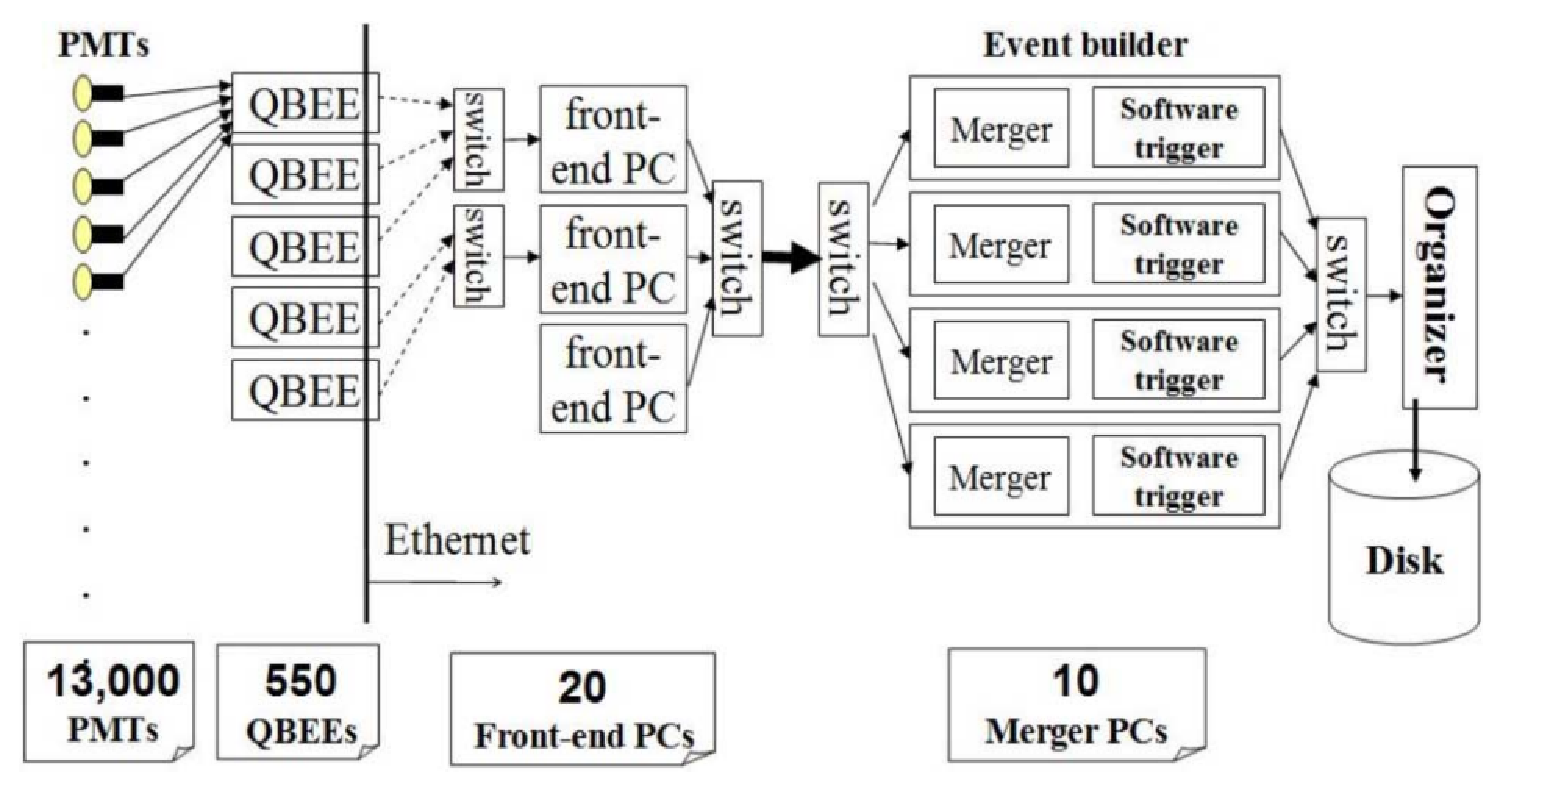
\includegraphics[width=\textwidth, trim={0mm 0mm 0mm 0mm}, clip,page=1]{Figures/Detectors/SKDataFlow.pdf}
  \end{subfigure}
  \caption{Schematic view of the data flow through the data acquisition and online system. Taken from \cite{5446533}.}
  \label{fig:T2KSKExp_SK_DataFlow}
\end{figure}

%The software trigger applied in SK-IV replaces the hardware trigger applied in SK-I to SK-III.
The software trigger (described in \cite{Yamada2007-cp}) operates by determining the number of PMT hits within a \quickmath{200\text{ns}} sliding window, \quickmath{N_{200}}. This window coincides with the maximum time that a Cherenkov photon would take to traverse the length of the SK tank \cite{PhysRevD.73.112001}. For lower energy events that generate fewer photons, this technique is useful for eliminating background processes like dark noise and radioactive decay which would be expected to separate in time. When the value of \quickmath{N_{200}} exceeds some threshold, a software trigger is issued. There are several trigger thresholds used within the SK-IV period which are detailed in \autoref{tab:T2KSKExp_TriggerThreshold}. If one of these thresholds is met, the PMT hits within an extended time window are also read out and saved to disk.
%The length of the time window is also included in the tabulated threshold conditions.
In the special case of an event that exceeds the SHE trigger but does not exceed the OD trigger, the AFT trigger looks for delayed coincidences of \quickmath{2.2 \text{MeV}} gamma rays emitted from neutron capture in a \quickmath{535 \mu\text{s}} window after the SHE trigger. A similar but more complex ``Wideband Intelligent Trigger (WIT)'' has been deployed and is described in \cite{Carminati2015-zx}.

\begin{table}[ht!]
    \centering
    \begin{tabular}{l|c|c|c}
      \hline
      Trigger & Acronym & Condition & Extended time window (\quickmath{\mu \text{s}}) \\
      \hline
      Super Low Energy & SLE & >34/31 hits & 1.3 \\
      Low Energy & LE & >47 hits & 40 \\
      High Energy & HE & >50 hits & 40 \\
      Super High Energy & SHE & >70/58 hits & 40 \\
      Outer Detector & OD & >22 hits in OD & N/A \\
      \hline
      \hline
    \end{tabular}
    \caption{The trigger thresholds and extended time windows saved around an event which were utilised throughout the SK-IV period. The exact thresholds can change and the values listed here represent the thresholds at the start and end of the SK-IV period.}
    \label{tab:T2KSKExp_TriggerThreshold}
\end{table}

\subsection{Cherenkov Radiation}
\label{subsec:T2KSKExp_Cherenkov}

Cherenkov light is emitted from any highly energetic charged particle traveling with relativistic velocity, \quickmath{\beta}, greater than the local speed of light in a medium \cite{Cerenkov1937-tl}.
%with refractive index \quickmath{n>1.0} 
%This occurs due to the charged particle exciting the polarised media, which de-excites via photon emission. From Huygen's principal, the emitted waves propagate outwards but only generate coherent wavefronts when the charged particle moves faster than the phase velocity of that media. Consequently,
Cherenkov light is formed at the surface of a cone with characteristic pitch angle,

\begin{equation}
  \label{eq:T2KSKExp_CherenkovConeAngle}
  \cos(\theta)=\frac{1}{\beta n}.
\end{equation}

where \quickmath{n} is the refractive index of the medium. Consequently, the Cherenkov momentum threshold, \quickmath{P_{thres}}, is dependent upon the mass, \quickmath{m}, of the charged particle moving through the medium, 

\begin{equation}
  P_{thres} = \frac{m}{\sqrt{n^{2}-1}}
\end{equation}

For water, where \quickmath{n = 1.33}, the Cherenkov threshold momentum and energy for various particles are given in \autoref{tab:T2KSKExp_CherenkovThreshold}. In contrast, \quickmath{\gamma}-rays are detected indirectly via the combination of photons generated by Compton scattering and pair production. The threshold for detection in the SK detector is typically higher than the threshold for photon production. This is due to the fact that the attenuation of photons in the water means that typically \quickmath{\sim 75\%} of Cherenkov photons reach the ID PMTs. Then the collection and quantum efficiencies described in \autoref{subsec:T2KSKExp_SKDetector} result in the number of detected photons being lower than the number of photons which reach the PMTs. 

\begin{table}[ht!]
    \centering
    \begin{tabular}{l|c|c}
      \hline
      Particle & Threshold Momentum (MeV) & Threshold Energy (MeV)\\
      \hline
      Electron & 0.5828 & 0.7751 \\
      Muon & 120.5 & 160.3 \\
      Pion & 159.2 & 211.7 \\
      Proton & 1070.0 & 1423.1 \\
      \hline
      \hline
    \end{tabular}
    \caption{The threshold momentum and energy for a particle to generate Cherenkov light in ultrapure water, as calculated in \autoref{eq:T2KSKExp_CherenkovConeAngle} in ultrapure water which has refractive index \quickmath{n = 1.33}.}
    \label{tab:T2KSKExp_CherenkovThreshold}
\end{table}

The Frank-Tamm equation \cite{Frank1991-wj} describes the relationship between the number of Cherenkov photons generated per unit length, \quickmath{dN/dx}, the wavelength of the photons generated, \quickmath{\lambda}, and the relativistic velocity of the charged particle,

\begin{equation}
  \label{eq:T2KSKExp_FrankTammFormula}
  \frac{d^2N}{dxd\lambda} = 2\pi\alpha \left(1 - \frac{1}{n^2 \beta^2} \right)\frac{1}{\lambda^2} .
\end{equation}

where \quickmath{\alpha} is the fine structure constant. For a \quickmath{100\text{MeV}} momentum electron, approximately \quickmath{330} photons will be produced per centimeter in the \quickmath{300\text{nm} \leq \lambda \leq 700\text{nm}} region which the ID PMTs are most sensitive to \cite{Fukuda2003-ly}.

\section{The Tokai to Kamioka Experiment}
\label{sec:T2KSKExp_T2K}

The Tokai to Kamioka (T2K) experiment is a long-baseline neutrino oscillation experiment located in Japan. Proposed in the early 2000s \cite{jhf_loi, Itow2001-vw} to replace K2K \cite{The_K2K_Collaboration2001-oo}, T2K was designed to observe electron neutrino appearance whilst precisely measuring the oscillation parameters associated with muon neutrino disappearance \cite{t2k_proposal}. The experiment consists of a neutrino beam generated at the Japan Proton Accelerator Research Complex (J-PARC), a suite of near detectors situated \quickmath{280\text{m}} from the beam target, and the Super Kamiokande far detector positioned at a \quickmath{295\text{km}} baseline. The cross-section view of the T2K experiment is drawn in \autoref{fig:T2KSKExp_T2K_Overview}.

\begin{figure}[h]
  \begin{subfigure}[t]{0.95\textwidth}
    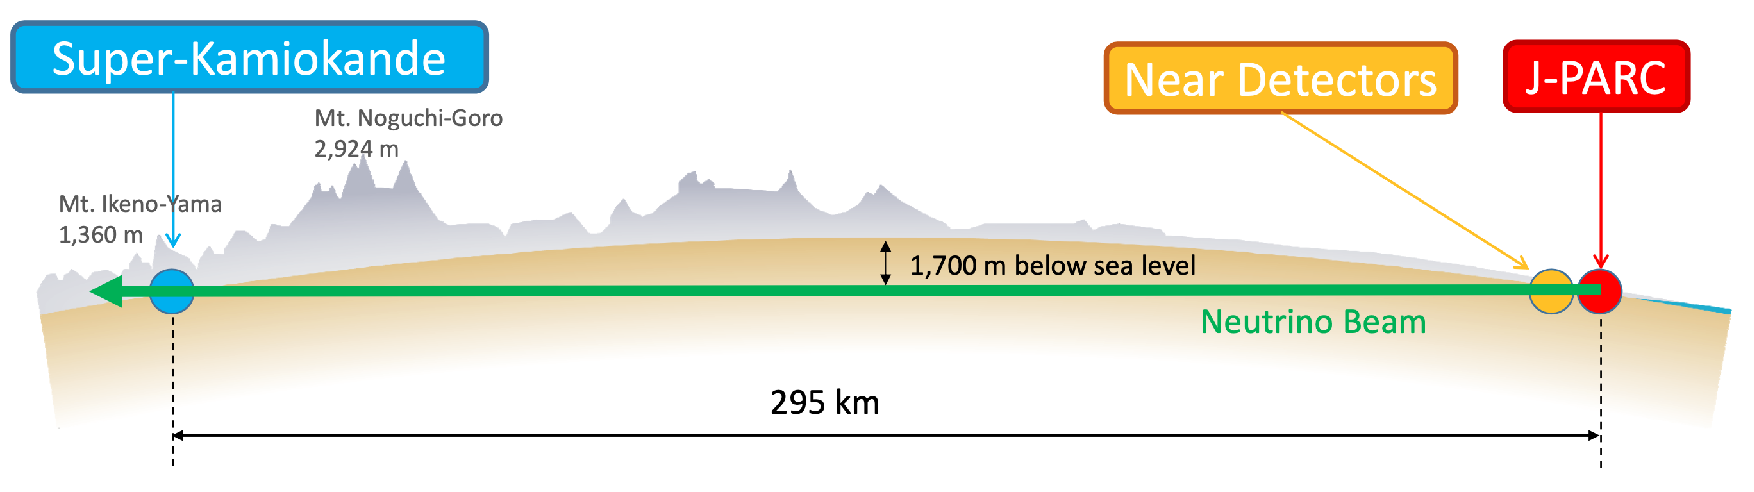
\includegraphics[width=\textwidth, trim={0mm 0mm 0mm 0mm}, clip,page=1]{Figures/Detectors/T2KCrossSection.pdf}
  \end{subfigure}
  \caption{The cross-section view of the Tokai to Kamioka experiment illustrating the beam generation facility at J-PARC, the near detector situated at a baseline of \quickmath{280\text{m}} and the Super Kamiokande far detector situated \quickmath{295\text{km}} from the beam target.}
  \label{fig:T2KSKExp_T2K_Overview}
\end{figure}

The T2K collaboration makes world-leading measurements of the \sinsqatm, \delmsqatm, and \dcp oscillation parameters. Improvements in the precision and accuracy of parameter estimates are still being made by including new data samples and developing the models which describe the neutrino interactions and detector responses \cite{Bronner2022-wd}. Electron neutrino appearance was first observed at T2K in 2014 \cite{2014_Abe_ElectronNuApp} with \quickmath{7.3\sigma} significance.

The near detectors provide constraints on the beam flux and cross-section model parameters used within the oscillation analysis by observing the unoscillated neutrino beam. There are a host of detectors situated in the near detector hall (As illustrated in \autoref{fig:T2KSKExp_T2K_ND280Pit}): ND280 (\autoref{subsec:T2KSKExp_T2K_ND280}), INGRID (\autoref{subsec:T2KSKExp_T2K_INGRID}), NINJA \cite{ninja}, WAGASCI \cite{wagasci}, and Baby-MIND \cite{baby_mind}. The latter three are not currently used within the oscillation analysis presented within this thesis.

\begin{figure}[h]
  \begin{subfigure}[t]{0.5\textwidth}
    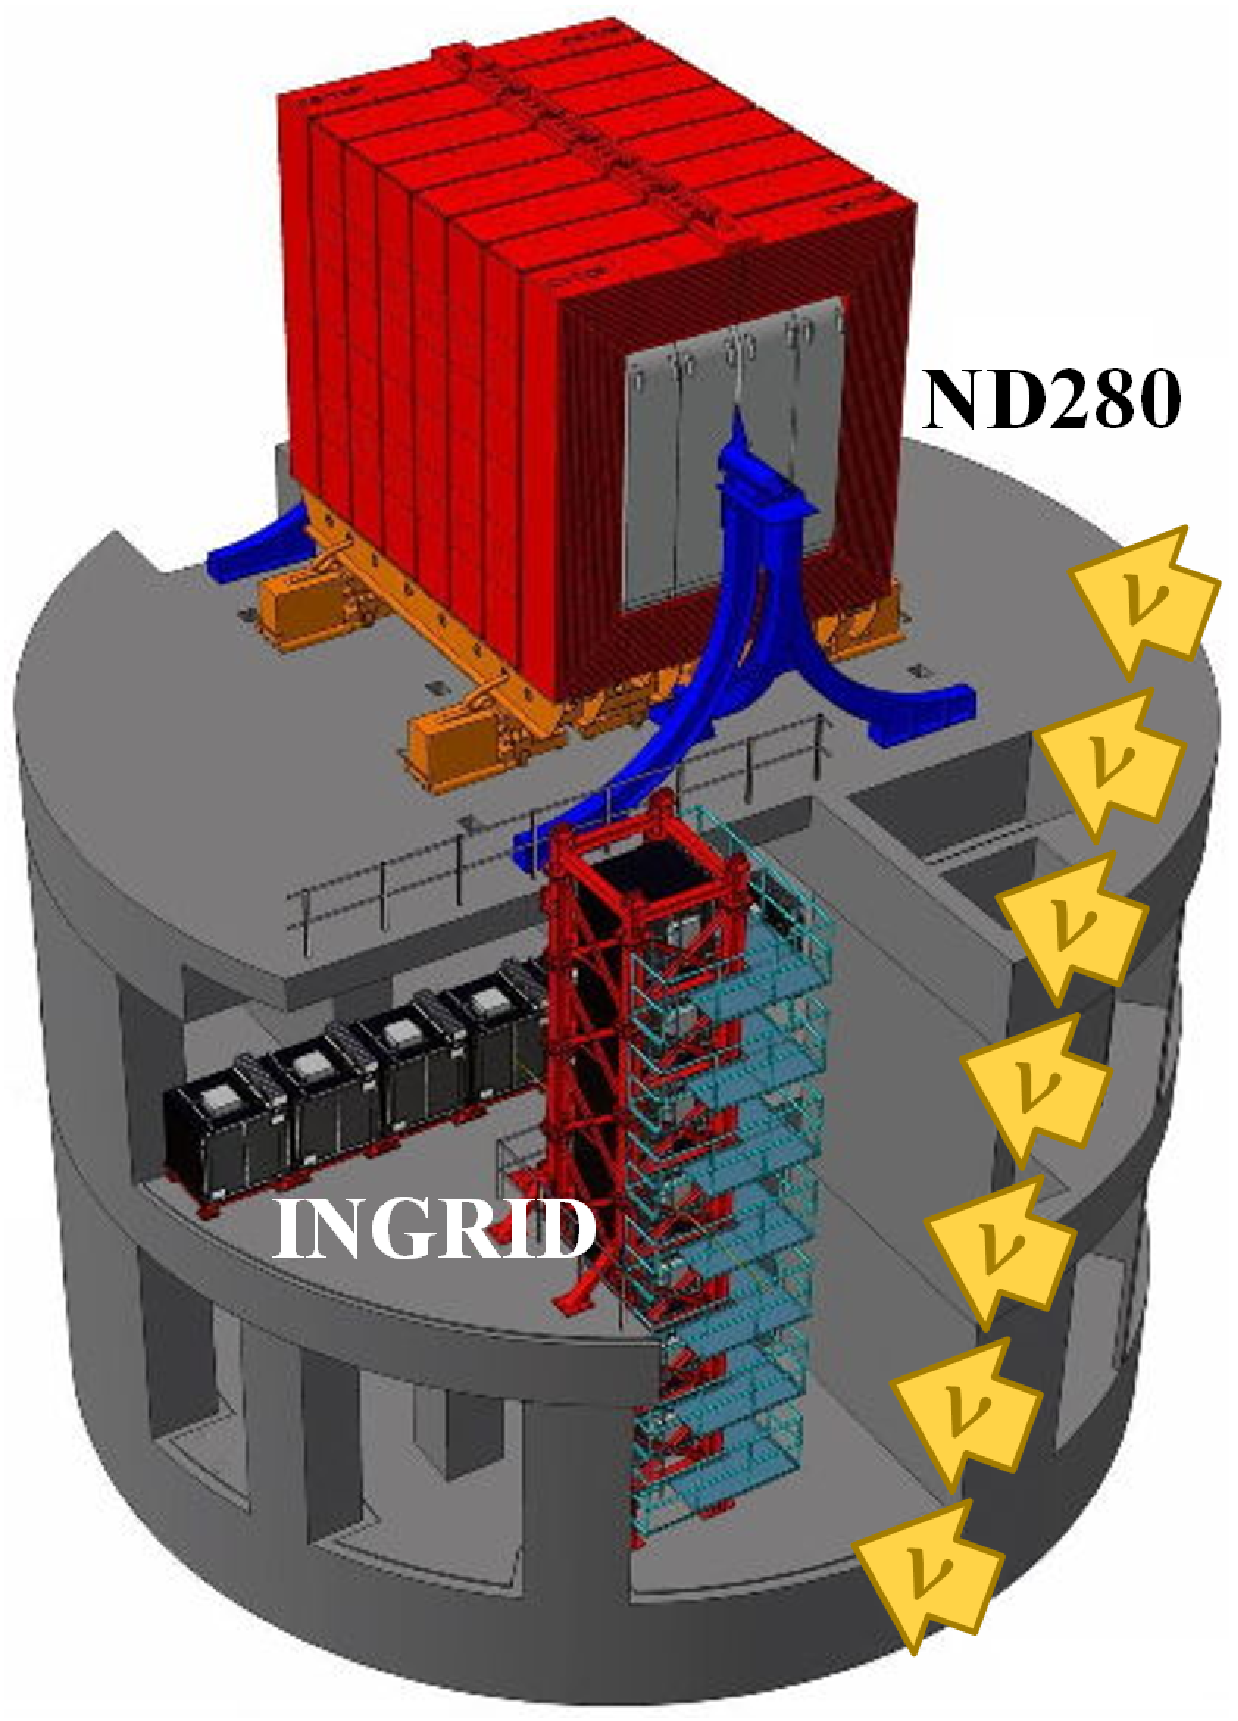
\includegraphics[width=\textwidth, trim={0mm 0mm 0mm 0mm}, clip,page=1]{Figures/Detectors/T2KND280Hall.pdf}
  \end{subfigure}
  \caption{The near detector suite for the T2K experiment showing the ND280 and INGRID detectors. The distance between the detectors and the beam target is \quickmath{280\text{m}}.}
  \label{fig:T2KSKExp_T2K_ND280Pit}
\end{figure}

Whilst this thesis presents the ND280 in terms of its purpose for the oscillation analysis, the detector can also make many cross-section measurements at neutrino energies of \quickmath{O(1)\text{GeV}} for the different targets within the detector \cite{PhysRevD.102.012007,10.1093/ptep/ptab014}. These measurements are of equal importance as they can lead the way in determining the model parameters used in the interaction models for the future high-precision era of neutrino physics.

There are two independent fitters, \texttt{MaCh3} and \texttt{BANFF}, which perform the near detector fit. \texttt{MaCh3} is the basis of this analysis and uses a bayesian Markov Chain Monte Carlo fitting technique, whereas \texttt{BANFF} uses a frequentist gradient descent technique. The output of each fitter is converted into a covariance matrix to describe the error and correlations between all the flux and cross-section parameters. This is then propagated to the far-detector oscillation analysis group for use in the \texttt{P-Theta} and \texttt{VALOR} fitting framework. As \texttt{MaCh3} can handle both near and far detector samples, it does not use this covariance matrix and instead opts for a simultaneous fit of the two detector measurements. This is an analysis choice which removes the assumption of Gaussian posterior distributions required when building the post-fit covariance matrix.

\finish{MaCh3 vs PTheta and Valor}

There are three particular tunes of the T2K flux and low energy cross section model typically considered. Firstly, the ``generated'' tune which is the set of dial values with which the Monte Carlo was generated. Secondly, the set of dial values which are taken from external data measurements and used as inputs. These are the ``pre-fit'' dial values. The reason these two sets of dial values are different is that the external data measurements are continually updated but it is very computationally intensive to regenerate a Monte Carlo prediction after each update. The final tune is the ``post-fit'', ``post-ND fit'' or ``post-BANFF'' dial values. These are the values taken from the fit to the beam near detector data.

\subsection{The Neutrino Beam}
\label{subsec:T2KSKExp_T2K_NeutrinoBeam}

The neutrino beam used within the T2K experiment is described in \cite{t2k_det, Abe_2013} and summarised below. The accelerating facility at J-PARC is composed of two sections; the primary and secondary beamlines. \autoref{fig:T2KSKExp_T2K_Beamline} illustrates a schematic of the beamline, focusing mostly on the components of the secondary beamline. The primary beamline has three accelerators that progressively accelerate protons; a linear accelerator, a rapid-cycling synchrotron, and the main-ring (MR) synchrotron. Once fully accelerated by the MR, the protons have a kinetic energy of \quickmath{30\text{GeV}}. Eight bunches of these protons, separated by \quickmath{500\text{ns}}, are extracted per ``spill'' from the MR and directed towards a graphite target (a rod of length \quickmath{91.4\text{cm}} and diameter \quickmath{2.6\text{cm}}).
Spills are extracted at \quickmath{~0.5\text{Hz}} with \quickmath{\sim 3\times10^{14}} protons contained per spill.
%A total of \quickmath{\sim 3\times 10^{14}} protons are contained in each spill. The rate of extracted spills is \quickmath{\sim 0.5\text{Hz}} although the width of the spill is \quickmath{\sim 5 \mu\text{s}}.

\begin{figure}[h]
  \begin{subfigure}[t]{0.7\textwidth}
    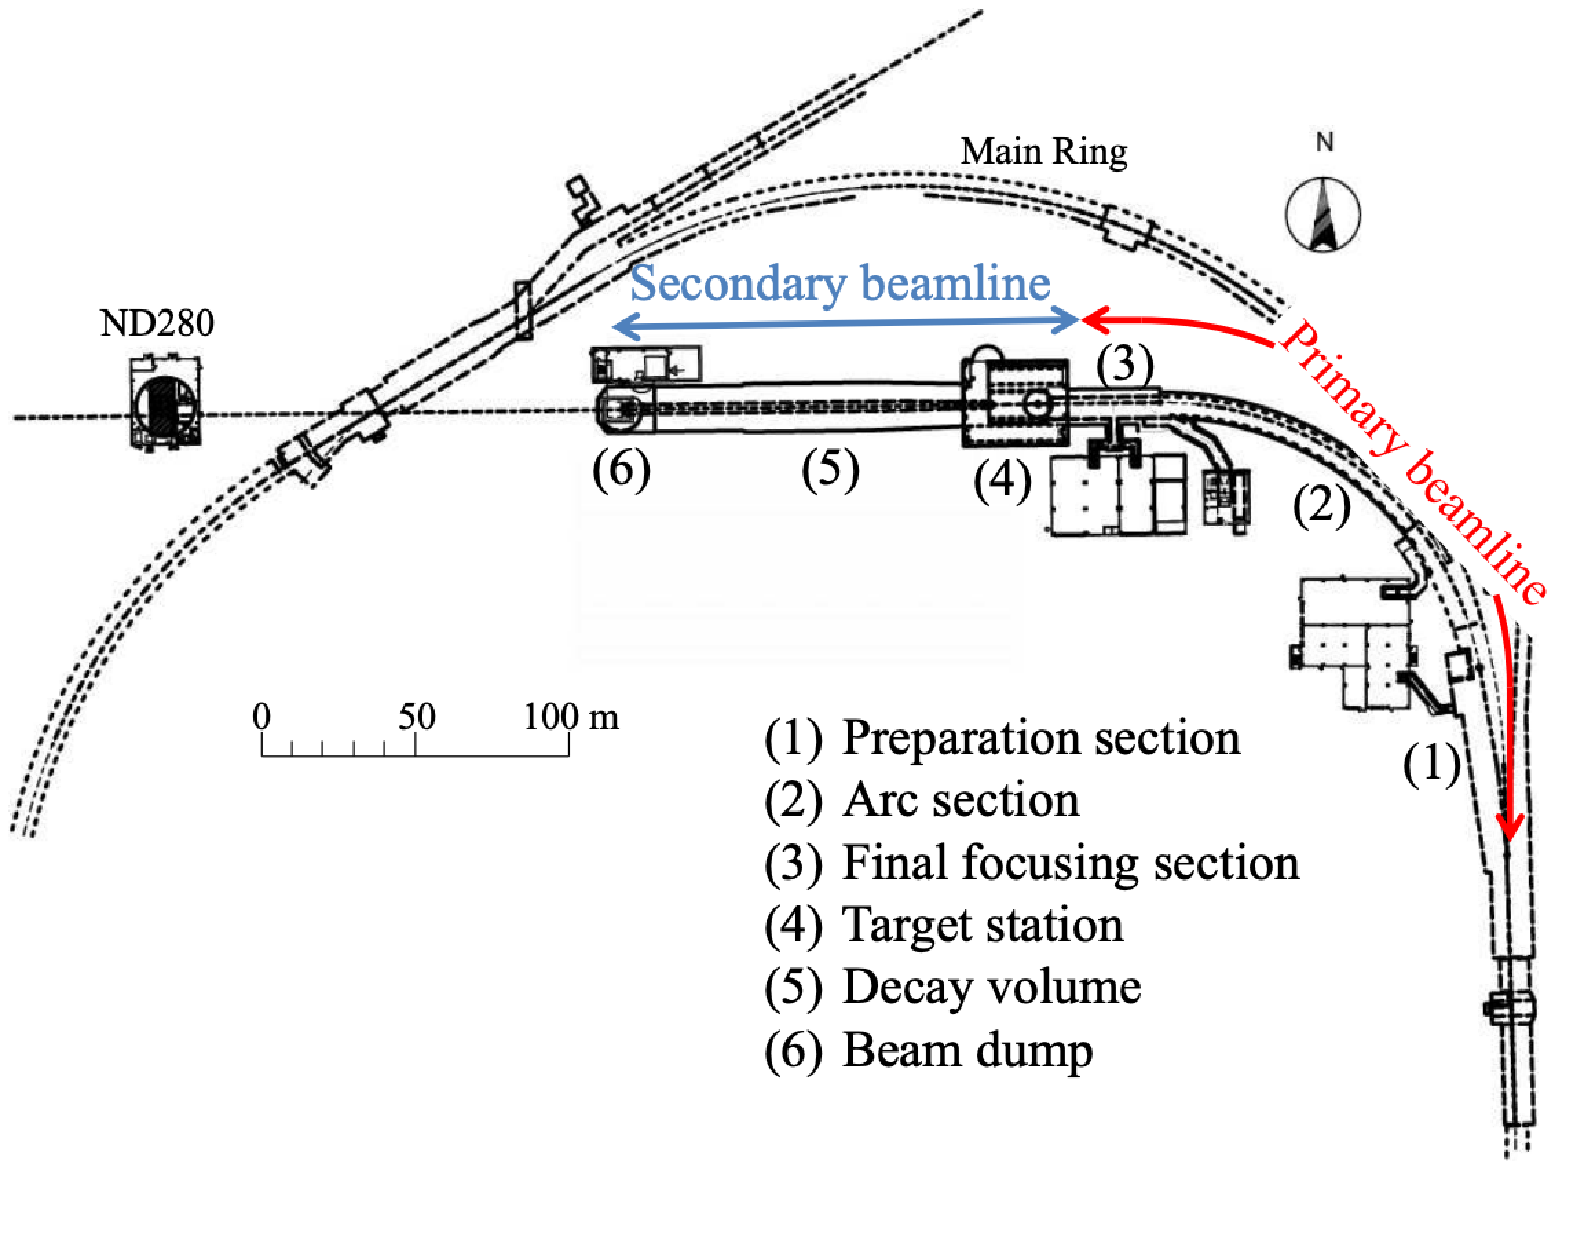
\includegraphics[width=\textwidth, trim={0mm 0mm 0mm 0mm}, clip,page=1]{Figures/Detectors/T2KBeamline.pdf}
    \subcaption{Primary and secondary beamline}
  \end{subfigure}
  \begin{subfigure}[t]{0.95\textwidth}
    \vspace{0.5cm}
    \includegraphics[width=\textwidth, trim={0mm 0mm 0mm 0mm}, clip,page=1]{Figures/Detectors/T2KSecondaryBeamline.pdf}
    \subcaption{Secondary beamline}
  \end{subfigure}
  \caption{Top panel: Bird's eye view of the most relevant part of primary and secondary beamline used within the T2K experiment. The primary beamline is the main-ring proton synchrotron, kicker magnet, and graphite target. The secondary beamline consists of the three focusing horns, decay volume, and beam dump. Figure taken from \cite{t2k_det}. Bottom panel: The side-view of the secondary beamline including the focusing horns, beam dump and neutrino detectors. Figure taken from \cite{MuMon}.}
  \label{fig:T2KSKExp_T2K_Beamline}
\end{figure}

The secondary beamline consists of three main components: the target station, the decay volume, and the beam dump. The target station is comprised of the target, beam monitors, and three magnetic focusing horns. The proton beam interacts with the graphite target to form a secondary beam of mostly pions and kaons. The secondary beam travels through a \quickmath{96\text{m}} long decay volume, generating neutrinos through the following decays \cite{Abe_2013},

\begin{minipage}{.45\linewidth}
  \begin{equation}
    \begin{split}
      \pi^+ &\rightarrow \mu^+ + \nu_\mu \\
      K^+ &\rightarrow \mu^+ + \nu_\mu \\
      &\rightarrow \pi^0 + e^+ + \nu_e \\
      &\rightarrow \pi^0 + \mu^+ + \nu_\mu \\
      K^0_L &\rightarrow \pi^- + e^+ + \nu_e \\
      &\rightarrow \pi^- + \mu^+ + \nu_\mu \\
      \mu^+ &\rightarrow e^+ + \bar{\nu}_\mu + \nu_e  \notag
    \end{split}
  \end{equation}
\end{minipage}%
\begin{minipage}{.45\linewidth}
  \begin{equation}
    \begin{split}
      \pi^- &\rightarrow \mu^- + \bar{\nu}_\mu\\
      K^- &\rightarrow \mu^- + \bar{\nu}_\mu \\
      &\rightarrow \pi^0 + e^- + \bar{\nu}_e\\
      &\rightarrow \pi^0 + \mu^- + \bar{\nu}_\mu \\
      K^0_L &\rightarrow \pi^+ + e^- + \bar{\nu}_e \\
      &\rightarrow \pi^+ + \mu^- + \bar{\nu}_\mu \\
      \mu^- &\rightarrow e^- + \nu_\mu + \bar{\nu}_e  \notag
    \end{split}
  \end{equation}
\end{minipage}

The electrically charged component of the secondary beam is focused towards the far detector by the three magnetic horns. These horns direct charged particles of a particular polarity towards SK whilst defocusing the oppositely charged particles. This allows a mostly neutrino or mostly antineutrino beam to be used within the experiment, denoted as ``forward horn current (FHC)'' or ``reverse horn current (RHC)'' respectively.

\autoref{fig:T2KSKExp_T2K_NuFluxPerMode} illustrates the different contributions to the FHC and RHC neutrino flux. The low energy flux is dominated by the decay of pions whereas kaon decay becomes the dominant source of neutrinos for \quickmath{E_\nu > 3\text{GeV}}. The ``wrong-sign'' component, which is the \quickmath{\bar{\nu}_\mu} background in a \quickmath{\nu_\mu} beam, and the intrinsic irreducible \quickmath{\nu_e} background, are predominantly due to muon decay for \quickmath{E_\nu < 2\text{GeV}}. As the antineutrino production cross-section is smaller than the neutrino cross-section, the wrong-sign component is more dominant in the RHC beam as compared to that in the FHC beam.

\begin{figure}[h]
  \begin{subfigure}[t]{0.45\textwidth}
    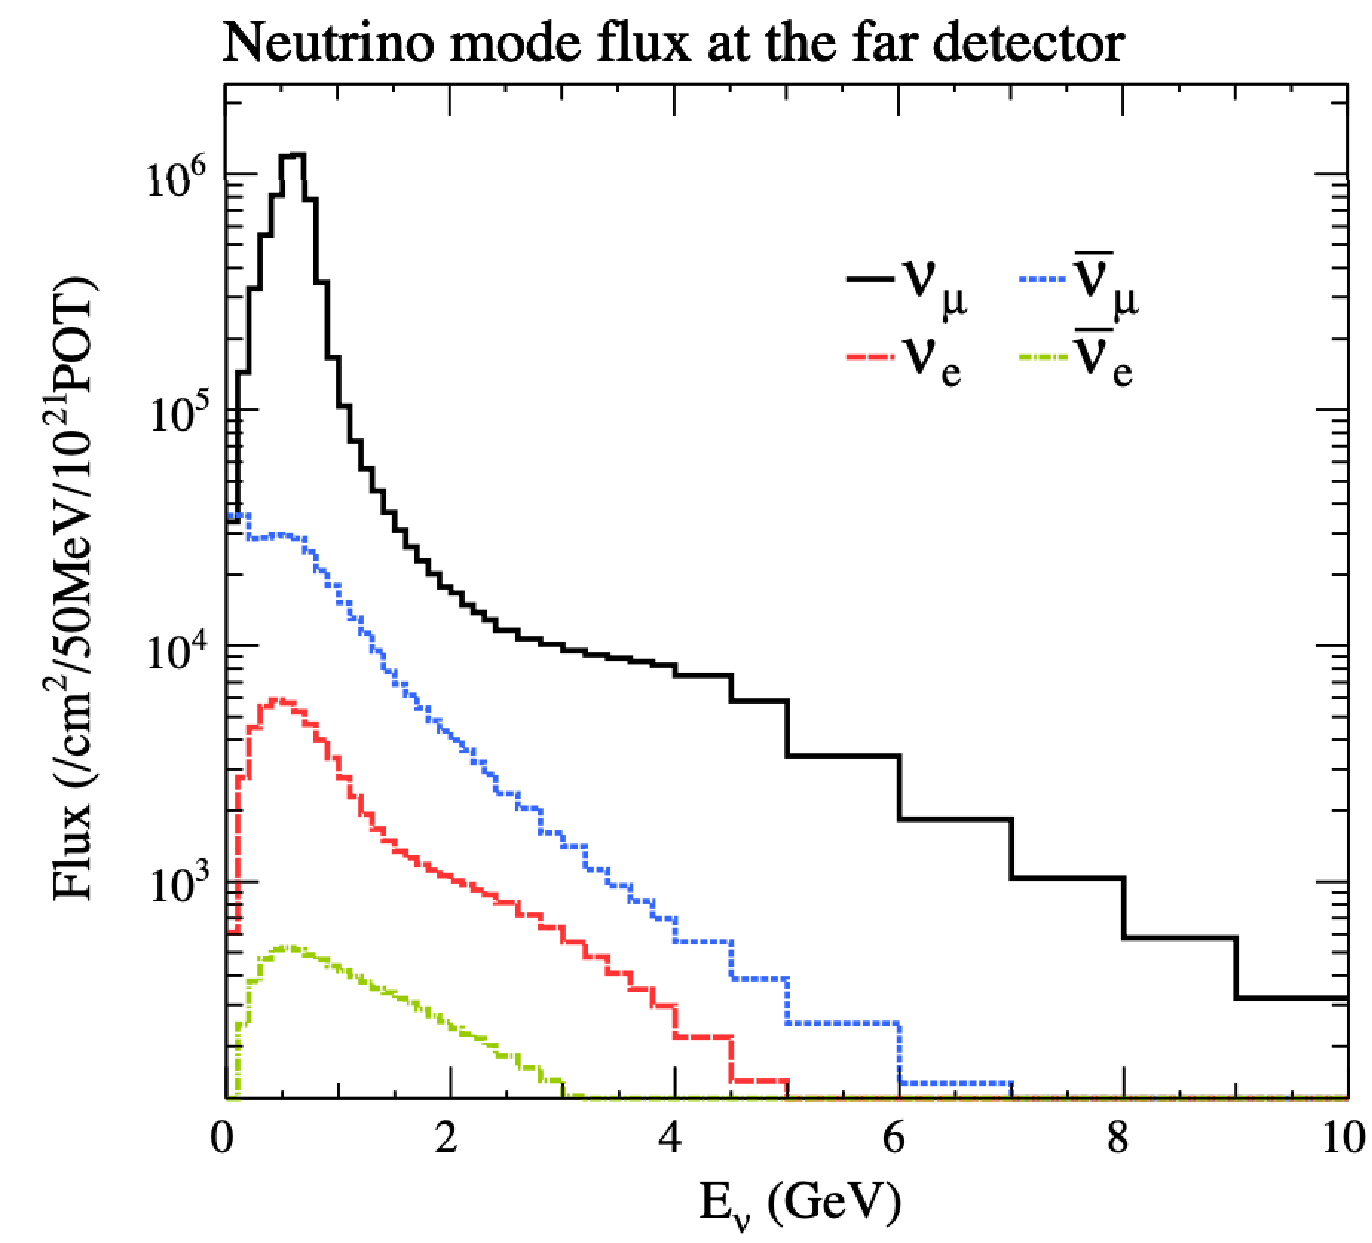
\includegraphics[width=\textwidth, trim={0mm 0mm 0mm 0mm}, clip,page=1]{Figures/Detectors/T2KFluxInNuMode.pdf}
  \end{subfigure}%
  \begin{subfigure}[t]{0.45\textwidth}
    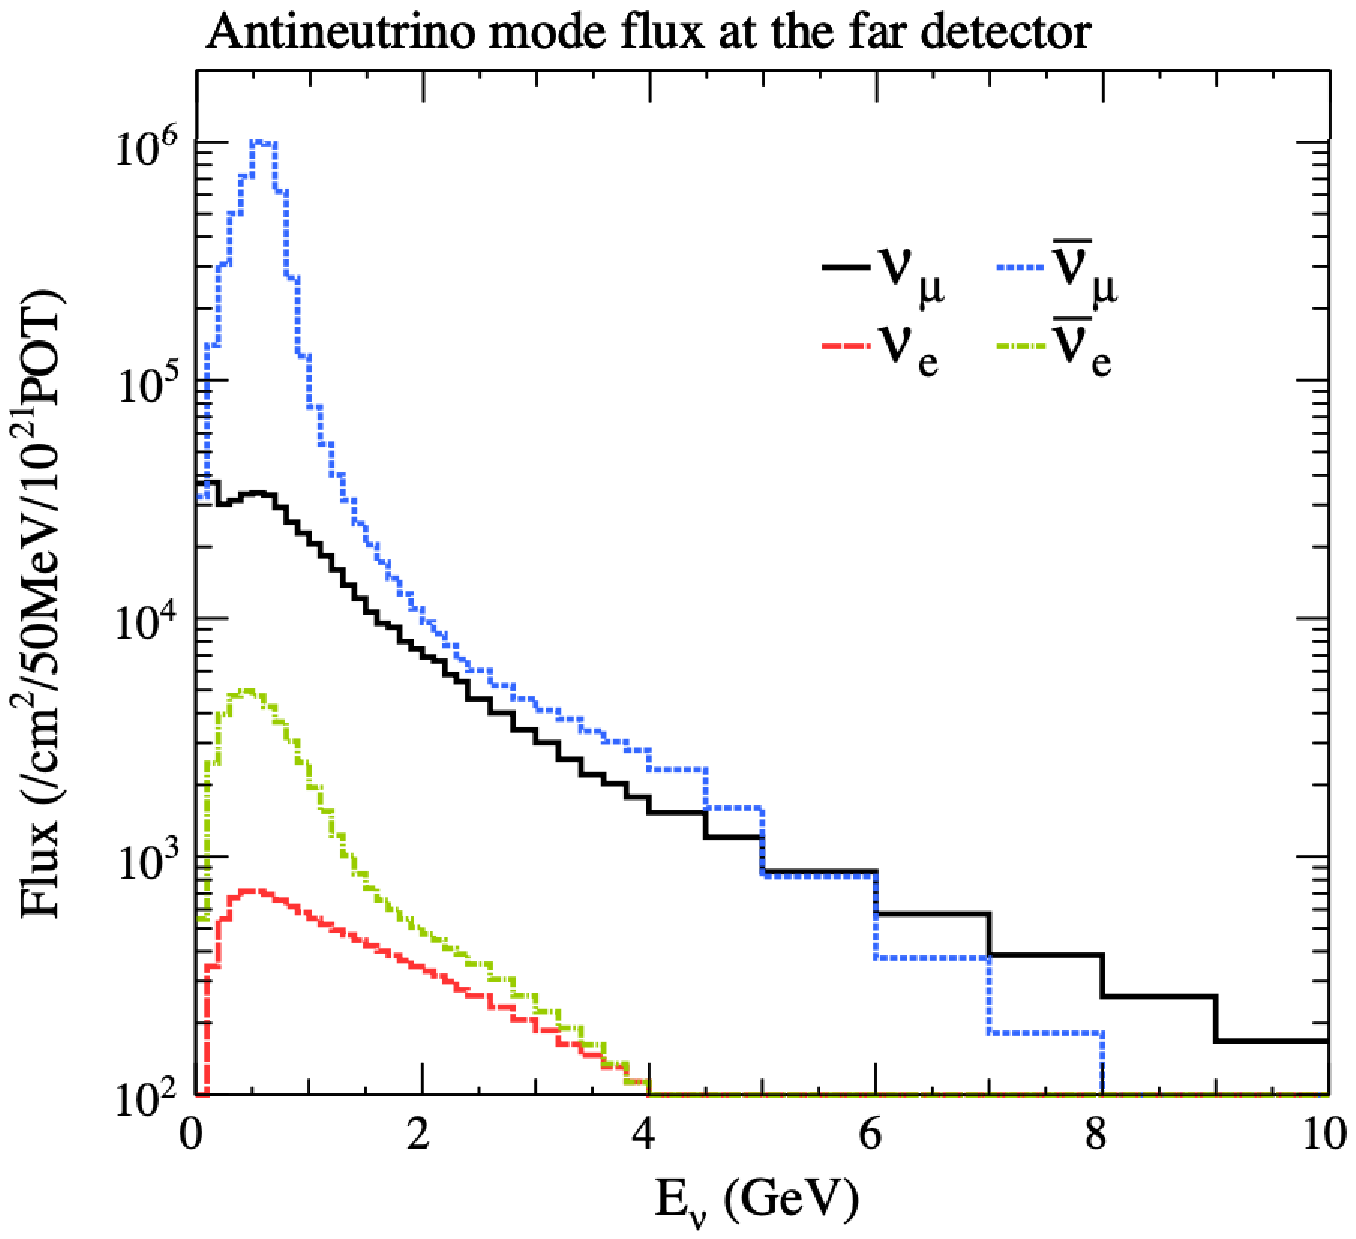
\includegraphics[width=\textwidth, trim={0mm 0mm 0mm 0mm}, clip,page=1]{Figures/Detectors/T2KFluxInANuMode.pdf}
  \end{subfigure}
  \caption{The Monte Carlo prediction of the energy spectrum for each flavour of neutrino (\quickmath{\nu_e}, \quickmath{\bar{\nu}_e}, \quickmath{\nu_\mu} and \quickmath{\bar{\nu}_\mu}) in the neutrino dominated beam FHC mode (Left) and antineutrino dominated beam RHC mode (Right) expected at SK. Taken from \cite{Abe2021-tr}.}
  \label{fig:T2KSKExp_T2K_NuFluxPerMode}
\end{figure}

The beam dump, situated at the end of the decay volume, stops all charged particles other than highly energetic muons (\quickmath{p_\mu > 5\text{GeV}}). The MuMon detector monitors the penetrating muons to determine the beam direction and intensity which is used to constrain some of the beam flux systematics within the analysis \cite{MuMon, Vladisavljevic2020-gv}. 

The T2K experiment uses an off-axis beam to narrow the neutrino energy distribution. This was the first implementation of this technique in a long-baseline neutrino oscillation experiment after its original proposal \cite{Beavis1995-qf}. Pion decay, \quickmath{\pi \rightarrow \mu + \nu_\mu}, is a two-body decay. Consequently, the neutrino energy, \quickmath{E_\nu}, can be determined based on the pion energy, \quickmath{E_\pi}, and the angle at which the neutrino is emitted, \quickmath{\theta},

\begin{equation}
  E_\nu = \frac{m^{2}_{\pi} - m^{2}_{\mu}}{2\left(E_\pi - p_\pi \cos(\theta) \right)},
\end{equation}

where \quickmath{m_{\pi}} and \quickmath{m_{\mu}} are the mass of the pion and muon respectively. For a fixed energy pion, the neutrino energy distribution is dependent upon the angle at which the neutrinos are observed from the initial pion beam direction. For the \quickmath{295\text{km}} baseline at T2K, \quickmath{E_\nu = 0.6\text{GeV}} maximises the electron neutrino appearance probability, \quickmath{P(\nu_\mu \rightarrow \nu_e)}, whilst minimising the muon disappearance probability, \quickmath{P(\nu_\mu \rightarrow \nu_\mu)}. \autoref{fig:T2KSKExp_T2K_OffAxisTrick} illustrates the neutrino energy distribution for a range of off-axis angles, as well as the oscillation probabilities most relevant to T2K.

\begin{figure}[h]
  \begin{subfigure}[t]{0.7\textwidth}
    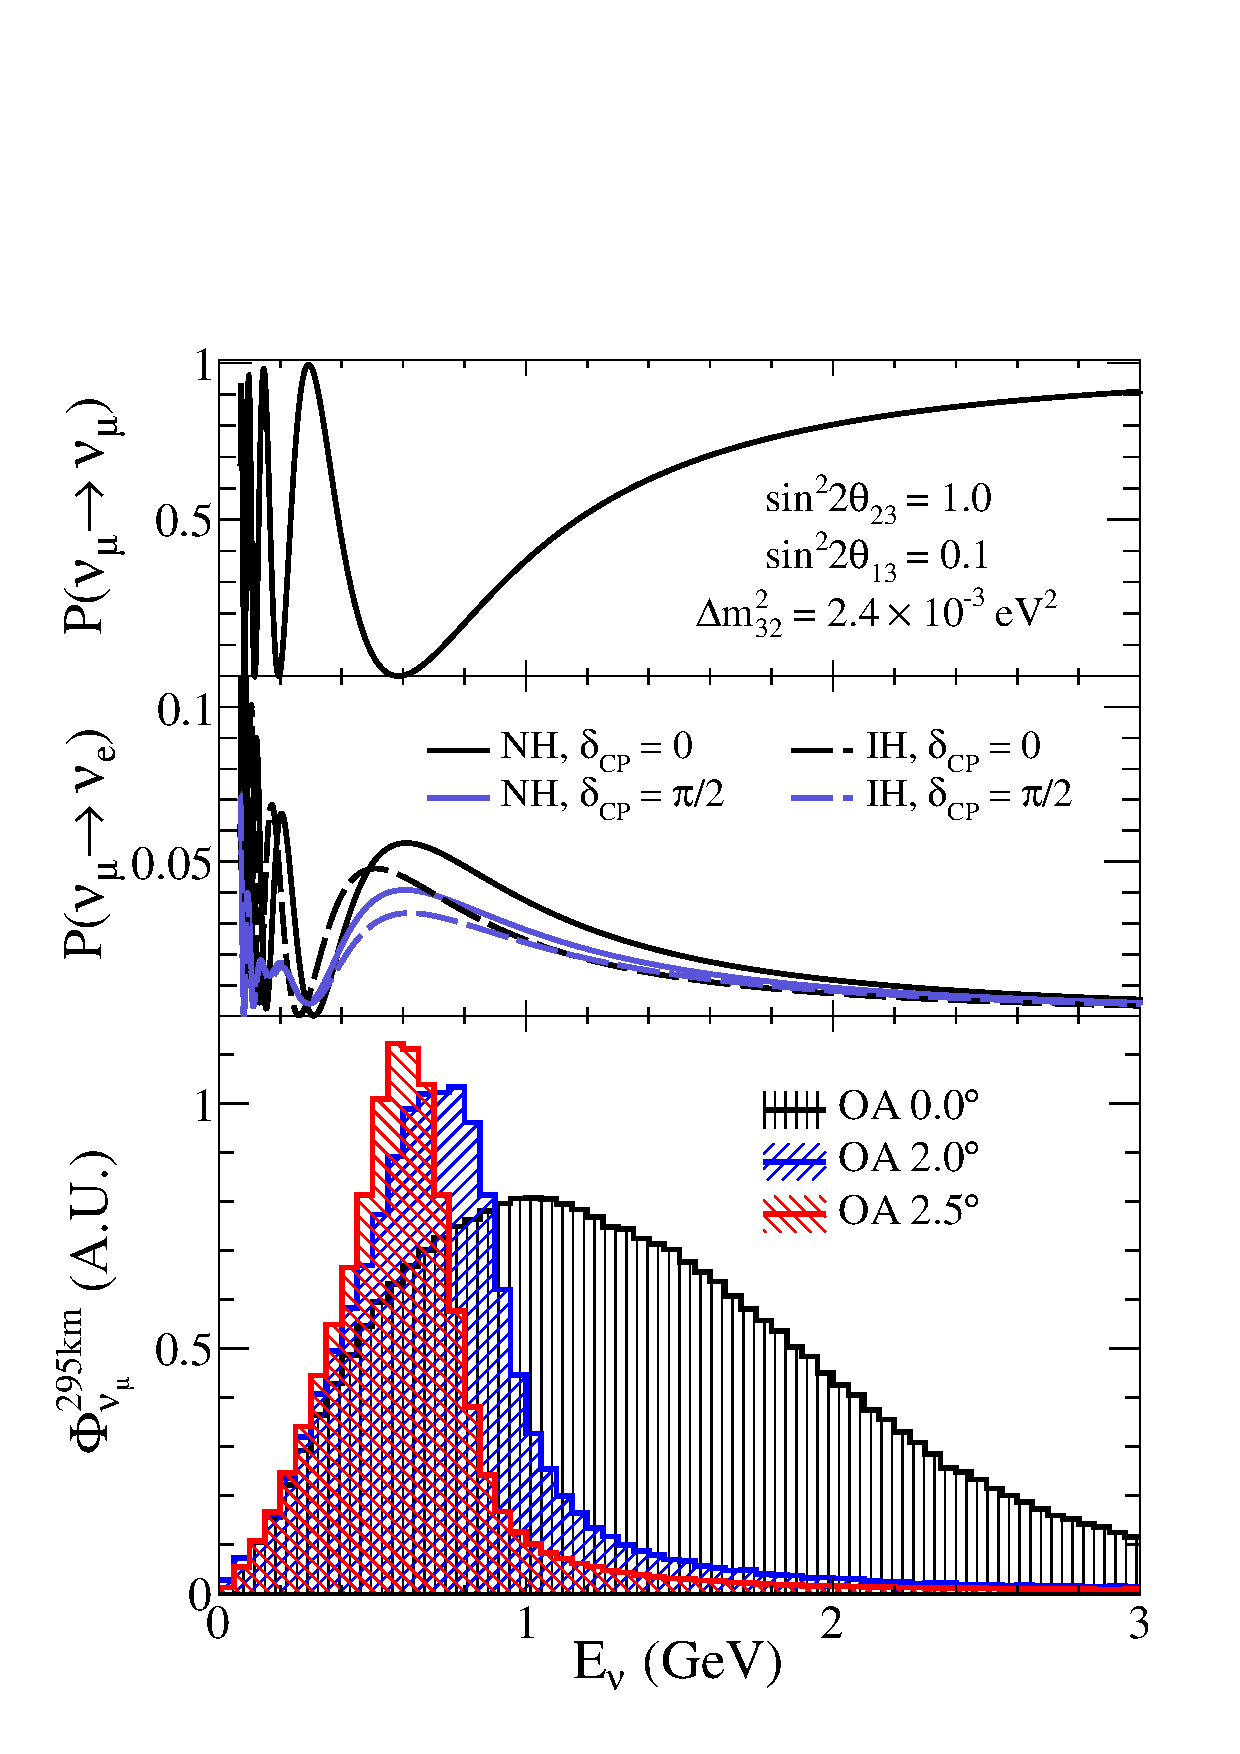
\includegraphics[width=\textwidth, trim={0mm 0mm 0mm 0mm}, clip,page=1]{Figures/Detectors/T2KOffAxisTrick.pdf}
  \end{subfigure}
  \caption{Top panel: T2K muon neutrino disappearance probability as a function of neutrino energy. Middle panel: T2K electron neutrino appearance probability as a function of neutrino energy. Bottom panel: The neutrino flux distribution for three different off-axis angles (Arbitrary units) as a function of neutrino energy.}
  \label{fig:T2KSKExp_T2K_OffAxisTrick}
\end{figure}

\subsection{The Near Detector at \quickmath{280\text{m}}}
\label{subsec:T2KSKExp_T2K_ND280}

Whilst all the near detectors are situated in the same ``pit'' located at \quickmath{280\text{m}} from the beamline, the ``ND280'' detector is the off-axis detector which is situated at the same off-axis angle as the Super-Kamiokande far detector. It has two primary functions; firstly it measures the neutrino flux and secondly it counts the event rates of different types of neutrino interactions. Both of these constrain the flux and cross-section systematics invoked within the model for a more accurate prediction of the expected event rate at the far detector.
%It is designed to observe the unoscillated neutrino flux to measure the beam flux whilst also counting the event rate of the different interaction modes in which a neutrino can interact through. This allows the systematics used within the model to be constrained for a more accurate prediction of the expected event rate at the far detector.

\begin{figure}[h]
  \begin{subfigure}[t]{0.7\textwidth}
    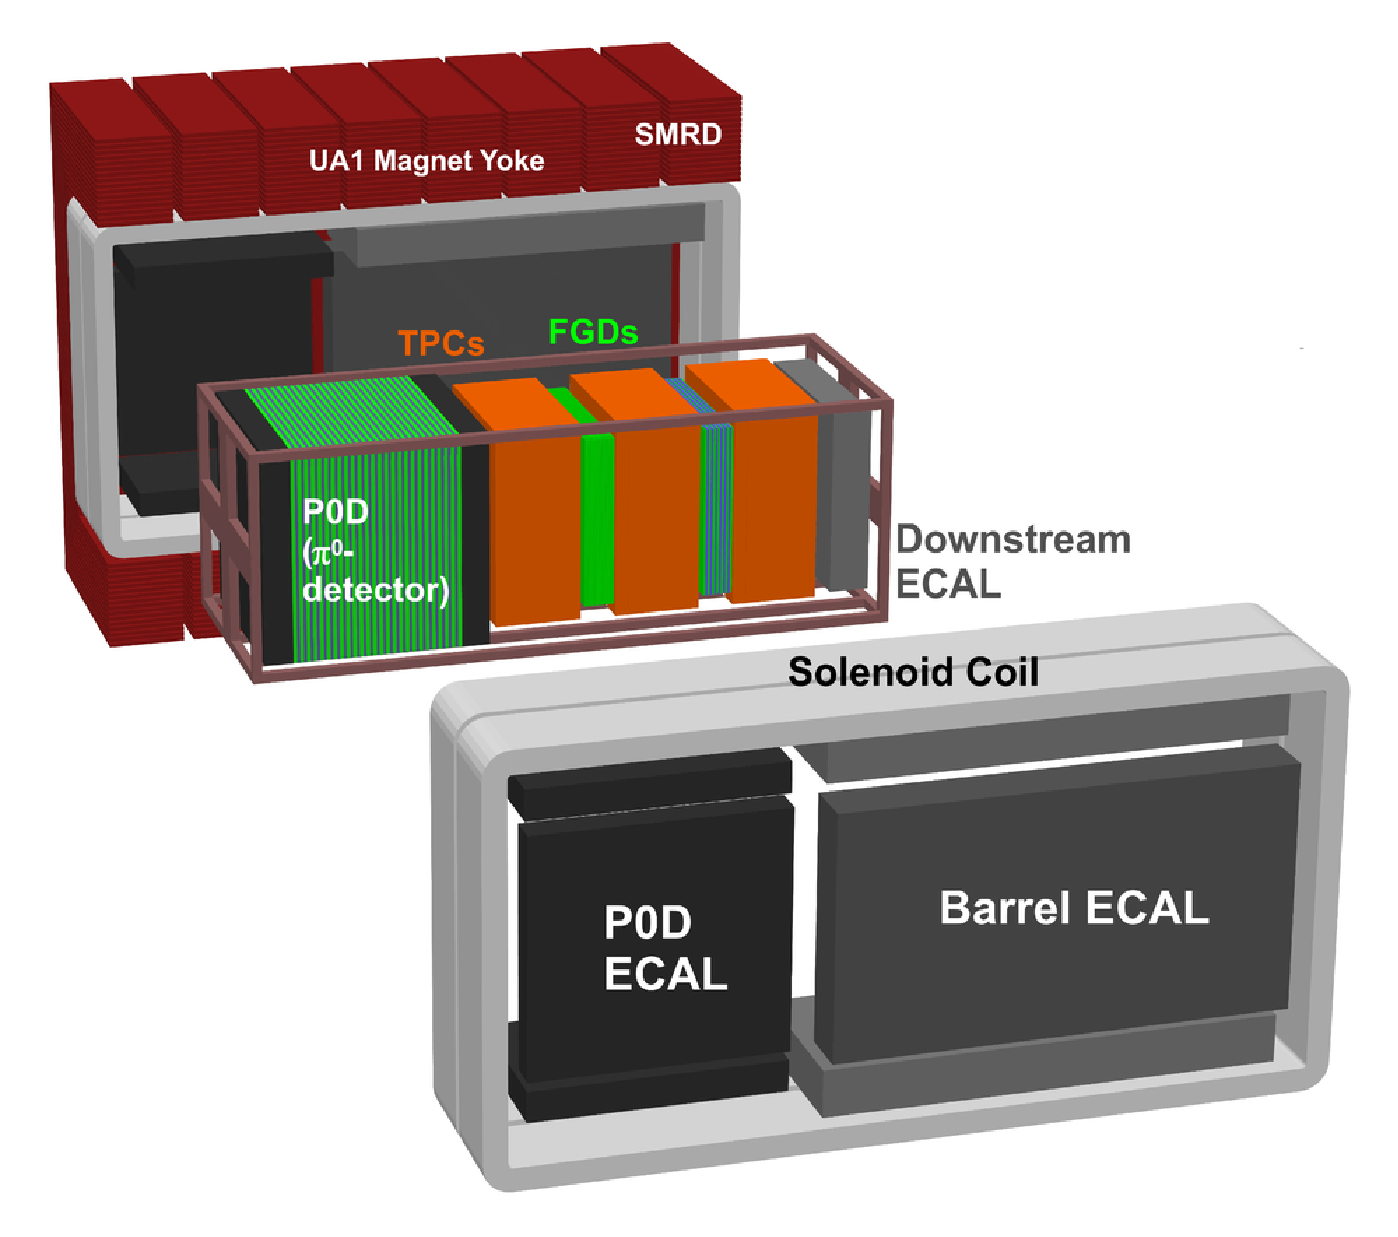
\includegraphics[width=\textwidth, trim={0mm 0mm 0mm 0mm}, clip,page=1]{Figures/Detectors/T2KND280.pdf}
  \end{subfigure}
  \caption{The components of the ND280 detector. The neutrino beam travels from left to right. Taken from \cite{t2k_det}.}
  \label{fig:T2KSKExp_T2K_ND280}
\end{figure}

As illustrated in \autoref{fig:T2KSKExp_T2K_ND280}, the ND280 detector consists of several sub-detectors. The most important part of the detector for this analysis is the tracker region. This is comprised of two time projection chambers (TPCs) sandwiched between three fine grain detectors (FGDs). The FGDs contain both hydrocarbon plastics and water targets for neutrino interactions and provide track reconstruction near the interaction vertex. The emitted charged particles can then propagate into the TPCs which provide particle identification and momentum reconstruction. The FGDs and TPCs are further described in \autoref{subsubsec:T2KSKExp_T2K_FGDs} and \autoref{subsubsec:T2KSKExp_T2K_TPCs} respectively. The electromagnetic calorimeter (ECAL) encapsulates the tracker region alongside the \quickmath{\pi^0} detector (P0D). The ECAL measures the deposited energy from photons emitted from interactions within the FGD. The P0D constrains the cross-section of neutral current interactions which generate neutral pions, which is one of the largest backgrounds in the electron neutrino appearance oscillation channel. The P0D and ECAL detectors are detailed in \autoref{subsubsec:T2KSKExp_T2K_P0D} and \autoref{subsubsec:T2KSKExp_T2K_ECAL} respectively. The entire detector is located within a large yoke magnet which produces a \quickmath{0.2\text{T}} magnetic field. This design of the magnet also includes a scintillating detector called the side muon range detector (SMRD) which is used to track high-angle muons as well as acting as a cosmic veto. The SMRD is described in \autoref{subsubsec:T2KSKExp_T2K_SMRD}.  

\subsubsection{Fine Grained Detectors}
\label{subsubsec:T2KSKExp_T2K_FGDs}

The T2K tracker region is comprised of two fine grained detectors (FGD) and three Time Projection Chambers (TPC). A detailed description of the FGD design, construction, and assembly is found in \cite{Amaudruz2012} and summarised below. The FGDs are the primary target for neutrino interactions with a mass of \quickmath{1.1} tonnes per FGD.
%material which are \quickmath{1.1} tonnes of target material per FDG for the neutrinos to interaction with.
Alongside this, the FGDs are designed to be able to track short-range particles which do not exit the FGD. Typically, short-range particles are low momentum and are observed as tracks that deposit a large amount of energy per unit length. This means the FGD needs good granularity to resolve these particles. The FGDs have the best timing resolution (\quickmath{\sim 3\text{ns}}) of any of the sub-detectors of the ND280 detector. As such, the FGDs are used for time of flight measurements to distinguish forward going positively charged particles from backward going negatively charged particles. Finally, any tracks which pass through multiple sub-detectors are required to be track matched to the FGD.

Both FGDs are made from square scintillator planes of side length \quickmath{186\text{cm}} and width \quickmath{2.02\text{cm}}. Each plane consists of two layers of 192 scintillator bars in an X or Y orientation. A wavelength shifting fiber is threaded through the centre of each bar and is read out by a multi-pixel photon counter (MPPC). FGD1 is the most upstream of the two FGDs and contains 15 planes of carbon plastic scintillator which is a common target in external neutrino scattering data. As the far detector is a pure water target, 7 of the 15 scintillator planes in FGD2 have been replaced with a hybrid water-scintillator target. Due to the complexity of the nucleus, nuclear effects can not be extrapolated between different nuclei. Therefore having the ability to take data on one target which is the same as external data and another target which is the same as the far detector target is beneficial for reliable model parameter estimates.

\begin{figure}[h]
  \begin{subfigure}[t]{0.7\textwidth}
    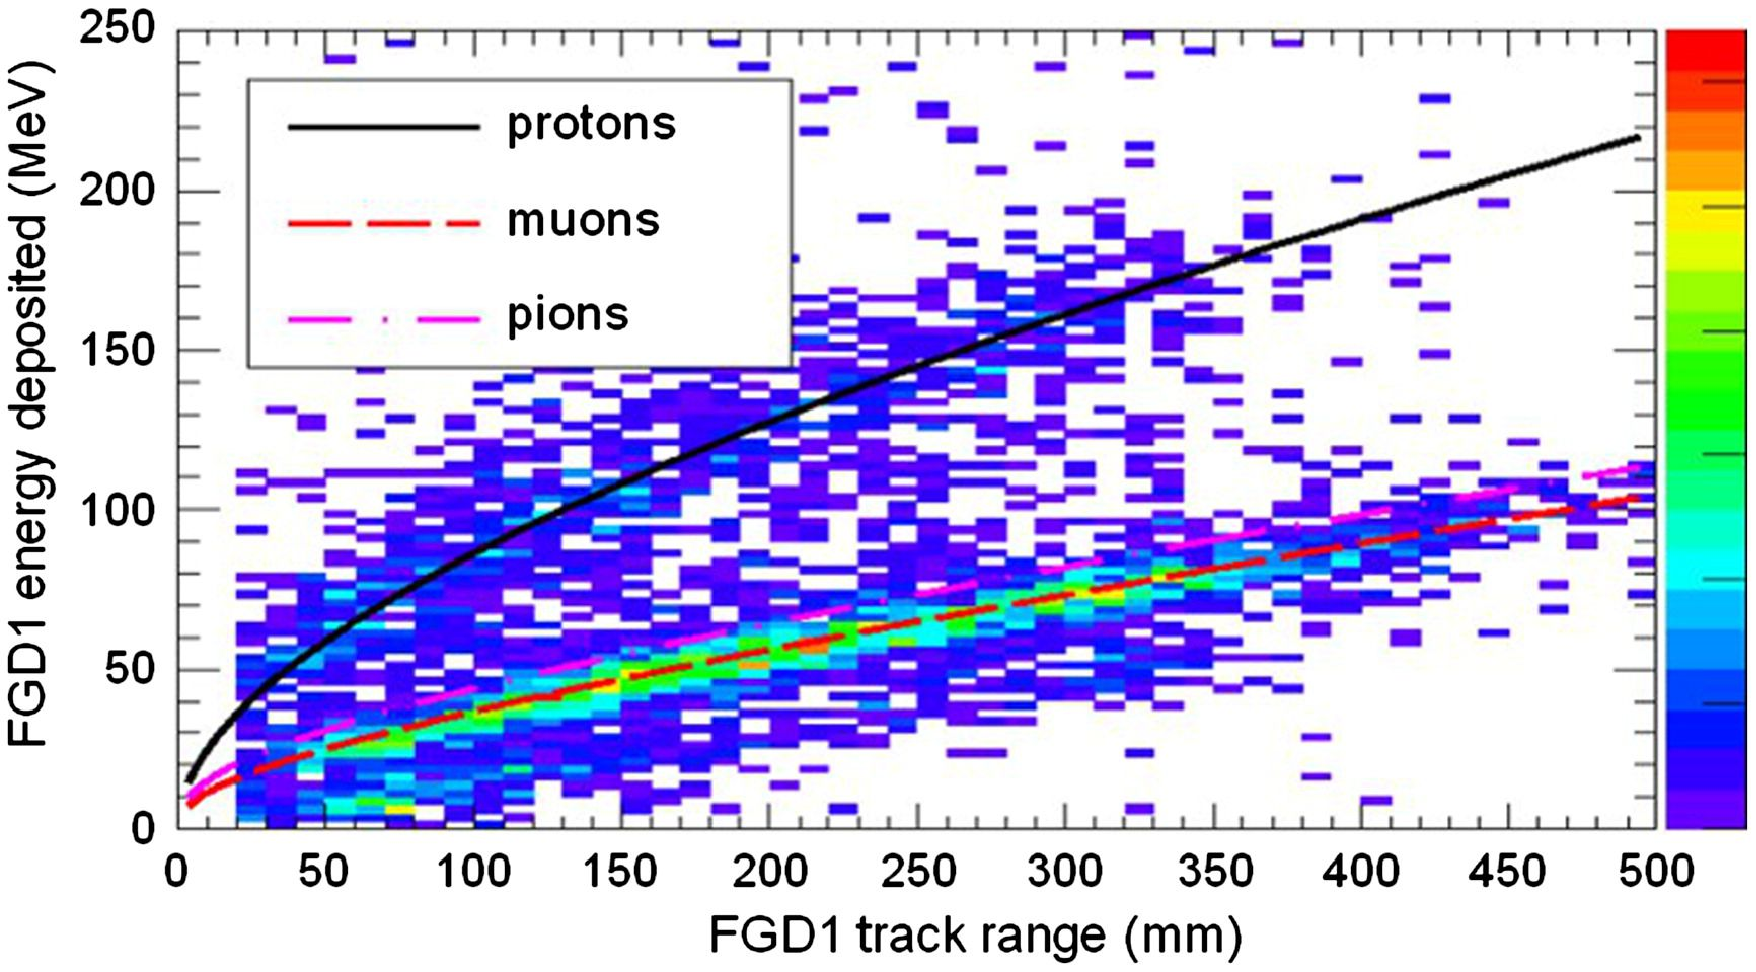
\includegraphics[width=\textwidth, trim={0mm 0mm 0mm 0mm}, clip,page=1]{Figures/Detectors/T2KFGDPID.pdf}
  \end{subfigure}
  \caption{Comparison of data to Monte Carlo prediction of integrated deposited energy as a function of track length for particles that stopped in FGD1. Taken from \cite{Amaudruz2012}.}
  \label{fig:T2KSKExp_T2K_FGDPID}
\end{figure}

The integrated deposited energy is used for particle identification. The FGD can distinguish protons from other charged particles by comparing the integrated deposited energy from data to Monte Carlo prediction as seen in \autoref{fig:T2KSKExp_T2K_FGDPID}.

\subsubsection{Time Projection Chambers}
\label{subsubsec:T2KSKExp_T2K_TPCs}

The majority of particle identification and momentum measurements within ND280 are provided by three Time Projection Chambers (TPCs) \cite{Abgrall2011}. The TPCs are located on either side of the FGDs. They are located inside of the magnetic field meaning the momentum of a charged particle can be determined from the bending of the track.
%They are designed with a momentum resolution of \quickmath{0.2\%} in order not to limit the determination of \delmsqatm at the far detector. Furthermore, to measure the intrinsic \quickmath{\nu_e} contamination of the beam, the resolution of the ionization energy loss is better than \quickmath{10\%} to ensure reliable particle identification.

Each TPC module consists of two gas-tight boxes, as shown in \autoref{fig:T2KSKExp_T2K_TPCDesign}, which are made of non-magnetic material. The outer box is filled with \quickmath{\text{CO}_2} which acts as an electrical insulator between the inner box and the ground. The inner box forms the field cage which produces a uniform electric drift field of \quickmath{\sim 275 \text{V/cm}} and is filled with an argon gas mixture. Charged particles moving through this gas mixture ionize the gas and the ionised charge is drifted towards micromegas detectors which measure the ionization charge. The time and position information in the readout allows a three-dimensional image of the neutrino interaction.

\begin{figure}[h]
  \begin{subfigure}[t]{0.55\textwidth}
    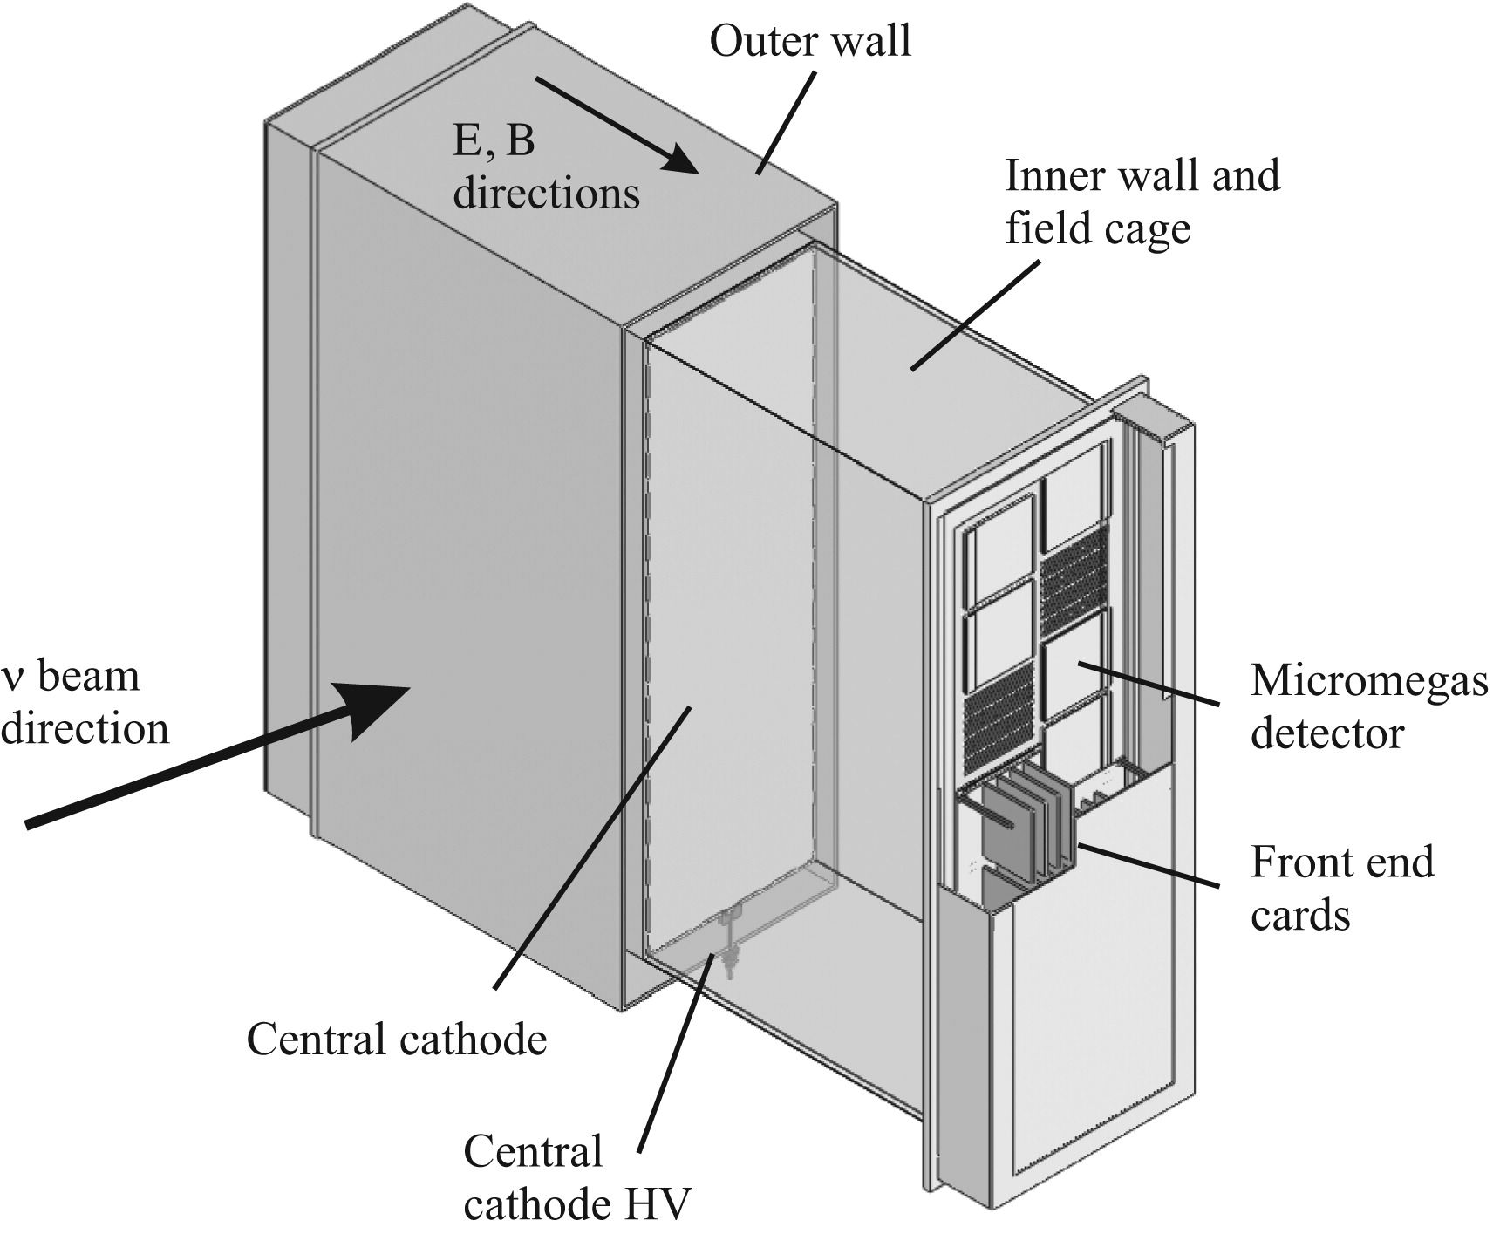
\includegraphics[width=\textwidth, trim={0mm 0mm 0mm 0mm}, clip,page=1]{Figures/Detectors/T2KTPCDesign.pdf}
  \end{subfigure}
  \caption{Schematic design of a Time Projection Chamber detector. Taken from \cite{Abgrall2011}.}
  \label{fig:T2KSKExp_T2K_TPCDesign}
\end{figure}

The particle identification of tracks that pass through the TPCs is performed using dE/dx measurements. \autoref{fig:T2KSKExp_T2K_TPC_dEdx} illustrates the data to Monte Carlo distributions of the energy lost by a charged particle passing through the TPC as a function of the reconstructed particle momentum. The resolution is \quickmath{7.8 \pm 0.2\%} meaning that electrons and muons can be distinguished. This allows reliable measurements of the intrinsic \quickmath{\nu_e} component of the beam.

\begin{figure}[h]
  \begin{subfigure}[t]{0.48\textwidth}
    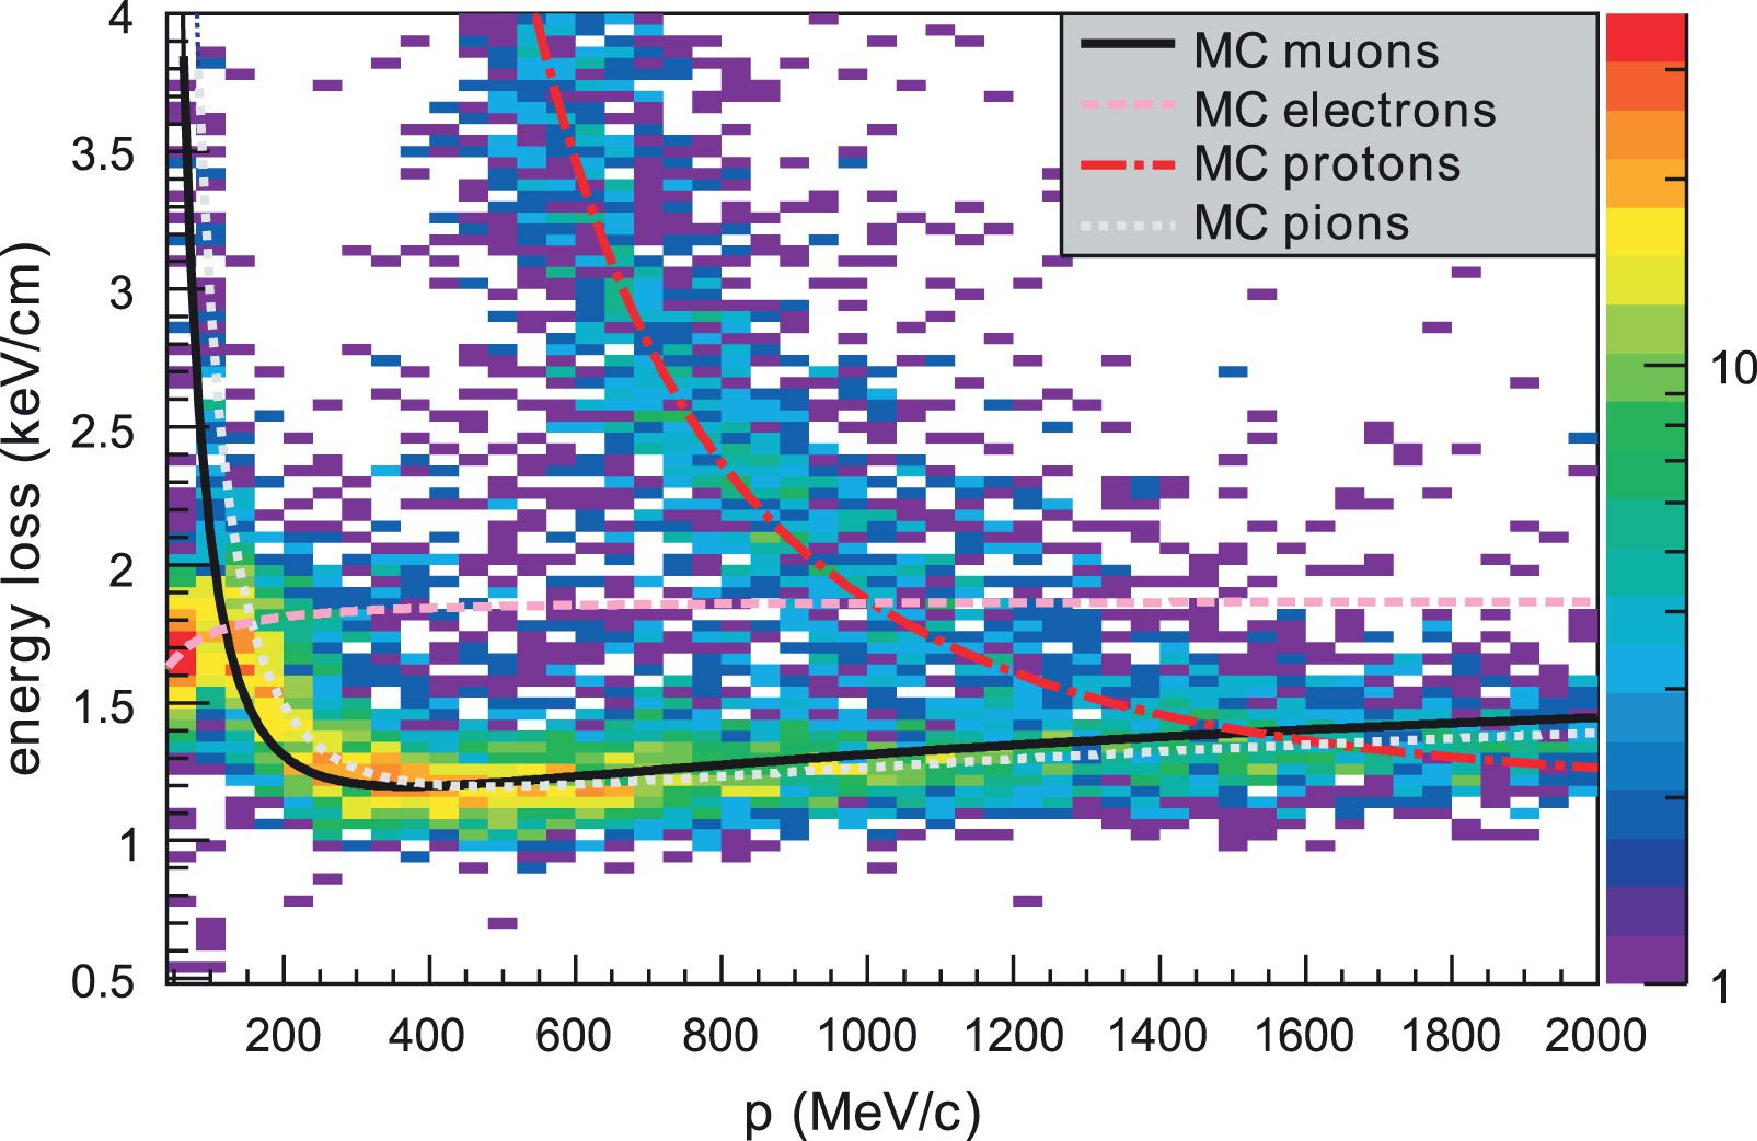
\includegraphics[width=\textwidth, trim={0mm 0mm 0mm 0mm}, clip,page=1]{Figures/Detectors/T2K_TPCdEdx_Positive.pdf}
    \subcaption{Positively charged particles}
  \end{subfigure}%
  \begin{subfigure}[t]{0.48\textwidth}
    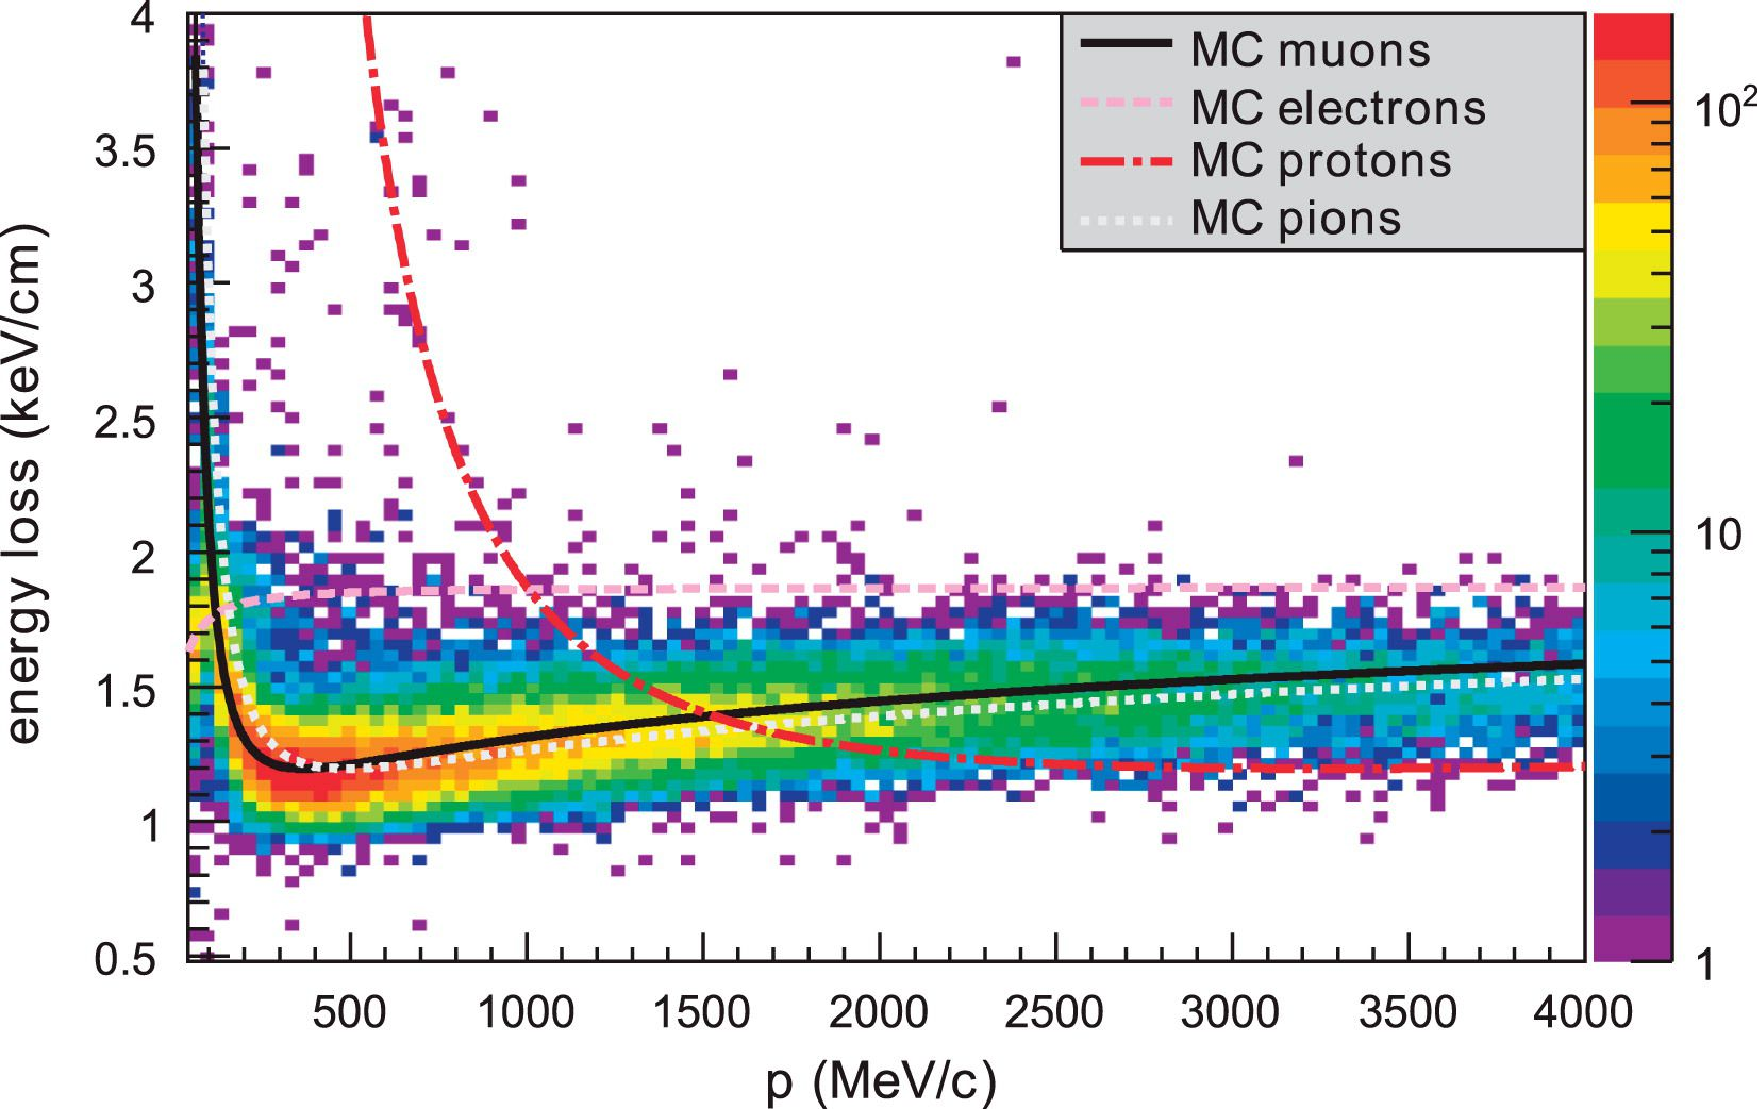
\includegraphics[width=\textwidth, trim={0mm 0mm 0mm 0mm}, clip,page=1]{Figures/Detectors/T2K_TPCdEdx_Negative.pdf}
    \subcaption{Negatively charged particles}
  \end{subfigure}
  \caption{The distribution of energy loss as a function of reconstructed momentum for charged particles passing through the TPC, comparing data to Monte Carlo prediction. Taken from \cite{Abgrall2011}.}
  \label{fig:T2KSKExp_T2K_TPC_dEdx}
\end{figure}

\subsubsection{\quickmath{\pi^0} Detector}
\label{subsubsec:T2KSKExp_T2K_P0D}

If one of the \quickmath{\gamma}-rays from a \quickmath{\pi^0 \rightarrow 2\gamma} decay is missed at the far detector, the reconstruction will determine that event to be a charge current \quickmath{\nu_{e}}-like event. This is one of the main backgrounds hindering the electron neutrino appearance searches. The \quickmath{\pi^0} detector (P0D) measures the cross-section of the neutral current induced neutral pion production on a water target to constrain this background.

The P0D is a cube of approximately \quickmath{2.5\text{m}} length consisting of layers of scintillating bars, brass and lead sheets, and water bags as illustrated in \autoref{fig:T2KSKExp_T2K_P0DDesign}. Two electromagnetic calorimeters are positioned at the most upstream and most downstream position in the sub-detector and the water target is situated in between them. The scintillator layers are built from two triangular bars orientated in opposite directions to form a rectangular layer. Each triangular scintillator bar is threaded with optical fiber which is read out by MPPCs. The high-Z brass and lead regions produce electron showers from the photons emitted in \quickmath{\pi^0} decay.

\begin{figure}[h]
  \begin{subfigure}[t]{0.55\textwidth}
    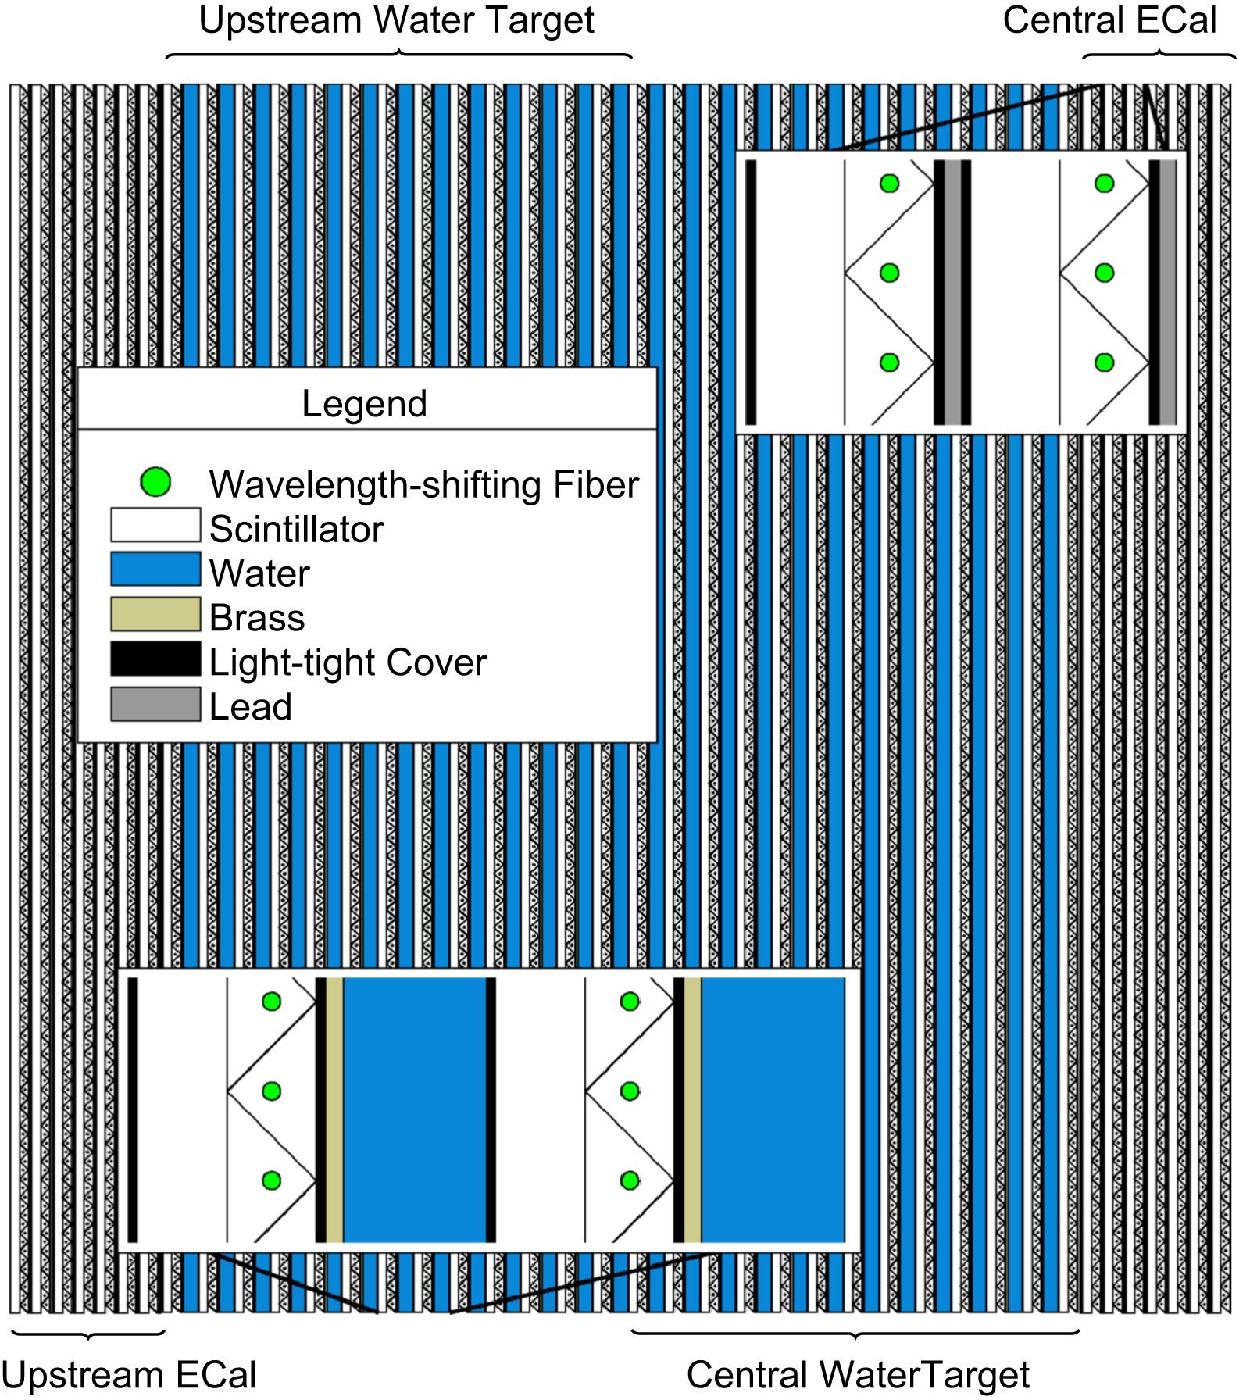
\includegraphics[width=\textwidth, trim={0mm 0mm 0mm 0mm}, clip,page=1]{Figures/Detectors/T2KP0DDesign.pdf}
  \end{subfigure}
  \caption{A schematic of the P0D side-view. Taken from \cite{Assylbekov2012}.}
  \label{fig:T2KSKExp_T2K_P0DDesign}
\end{figure}

The sub-detector can generate measurements of NC\quickmath{1\pi^0} cross-sections on a water target by measuring the event rate both with and without the water target, with the cross-section on a water target being determined as the difference. The total active mass is \quickmath{16.1} tonnes when filled with water and \quickmath{13.3} tonnes when empty.

\subsubsection{Electromagnetic Calorimeter}
\label{subsubsec:T2KSKExp_T2K_ECAL}

The electromagnetic calorimeter \cite{Allan_2013} (ECal) encapsulates the P0D and tracking sub-detectors. Its primary purpose is to aid \quickmath{\pi^0} reconstruction from any interaction in the tracker. To do this, it measures the energy and direction of photon showers from \quickmath{\pi^0 \rightarrow 2\gamma} decay. It can also distinguish pion and muon tracks depending on the shape of the photon shower deposited.

The ECal is comprised of three sections; the P0D ECal which surrounds the P0D, the barrel ECal which encompasses the tracking region, and the downstream ECal which is situated downstream of the tracker region. The barrel and downstream ECals are tracking calorimeters that focus on electromagnetic showers from high-angle particles emitted from the tracking sub-detectors. Particularly in  the TPC, high-angle tracks (those which travel perpendicularly to the beam-axis) can travel along a single scintillator bar resulting in very few hits. The width of the barrel and downstream ECal corresponds to \quickmath{\sim 11} electron radiation lengths to ensure a significant amount of the \quickmath{\pi^{0}} energy is contained. As the P0D has its own calorimetry which reconstructs showers, the P0D ECal determines the energy which escapes the P0D.

Each ECal is constructed of multiple layers of scintillating bars sandwiched between lead sheets. The scintillating bars are threaded with optical fiber and read out by MPPCs. Each sequential layer of the scintillator is orientated perpendicular to the previous which allows a three dimensional event reconstruction. The target mass of the P0D ECal, barrel ECal, and downstream ECal are \quickmath{1.50}, \quickmath{4.80} and \quickmath{6.62} tonnes respectively.

\subsubsection{Side Muon Range Detector}
\label{subsubsec:T2KSKExp_T2K_SMRD}

As illustrated in \autoref{fig:T2KSKExp_T2K_ND280}, the ECal, FGDs, P0D, and TPCs are enclosed within the UA1 magnet. Originally designed for the NOMAD \cite{Vannucci2014} experiment and reconditioned for use in the T2K experiment \cite{cerncourier_2022}, the UA1 magnet provides a uniform horizontal magnetic field of 0.2\text{T} with an uncertainty of \quickmath{2\times10^{-4}\text{T}}.

Built into the UA1 magnet, the side muon range detector (SMRD)\cite{Aoki2013} monitors high-energy muons which leave the tracking region and permeate through the ECal. It additionally acts as a cosmic muon veto and trigger. 

\subsection{The Interactive Neutrino GRID}
\label{subsec:T2KSKExp_T2K_INGRID}

The Interactive Neutrino GRID (INGRID) detector is situated within the same ``pit'' as the other near detectors. It is aligned with the beam in the ``on-axis'' position and measures the beam direction, spread, and intensity. The detector was originally designed with 16 identical modules \cite{t2k_det} (two modules have since been decommissioned) and a ``proton'' module. The design of the detector is cross-shaped with length and height \quickmath{10\text{m} \times 10\text{m}} as illustrated in \autoref{fig:T2KSKExp_T2K_INGRID}.

Each module is composed of iron sheets interlaced with eleven tracking scintillator planes for a total target mass of \quickmath{7.1} tonnes per module. The scintillator design is an X-Y pattern of 24 bars in both orientations, where each bar contains wave-length shifting fibers which are connected to multi-pixel photon counters (MPPCs). Each module is encapsulated inside veto planes to aid the rejection of charged particles entering the module.

The proton module is different from the other modules in that it consists of entirely scintillator planes with no iron target. The scintillator bars are also smaller than those used in the other modules to increase the granularity of the detector and improve tracking capabilities. The module sits in the centre of the beamline and is designed to give precise measurements of quasi-elastic charged current interactions to evaluate the performance of the Monte Carlo simulation of the beamline. 

\begin{figure}[h]
  \begin{subfigure}[t]{0.45\textwidth}
    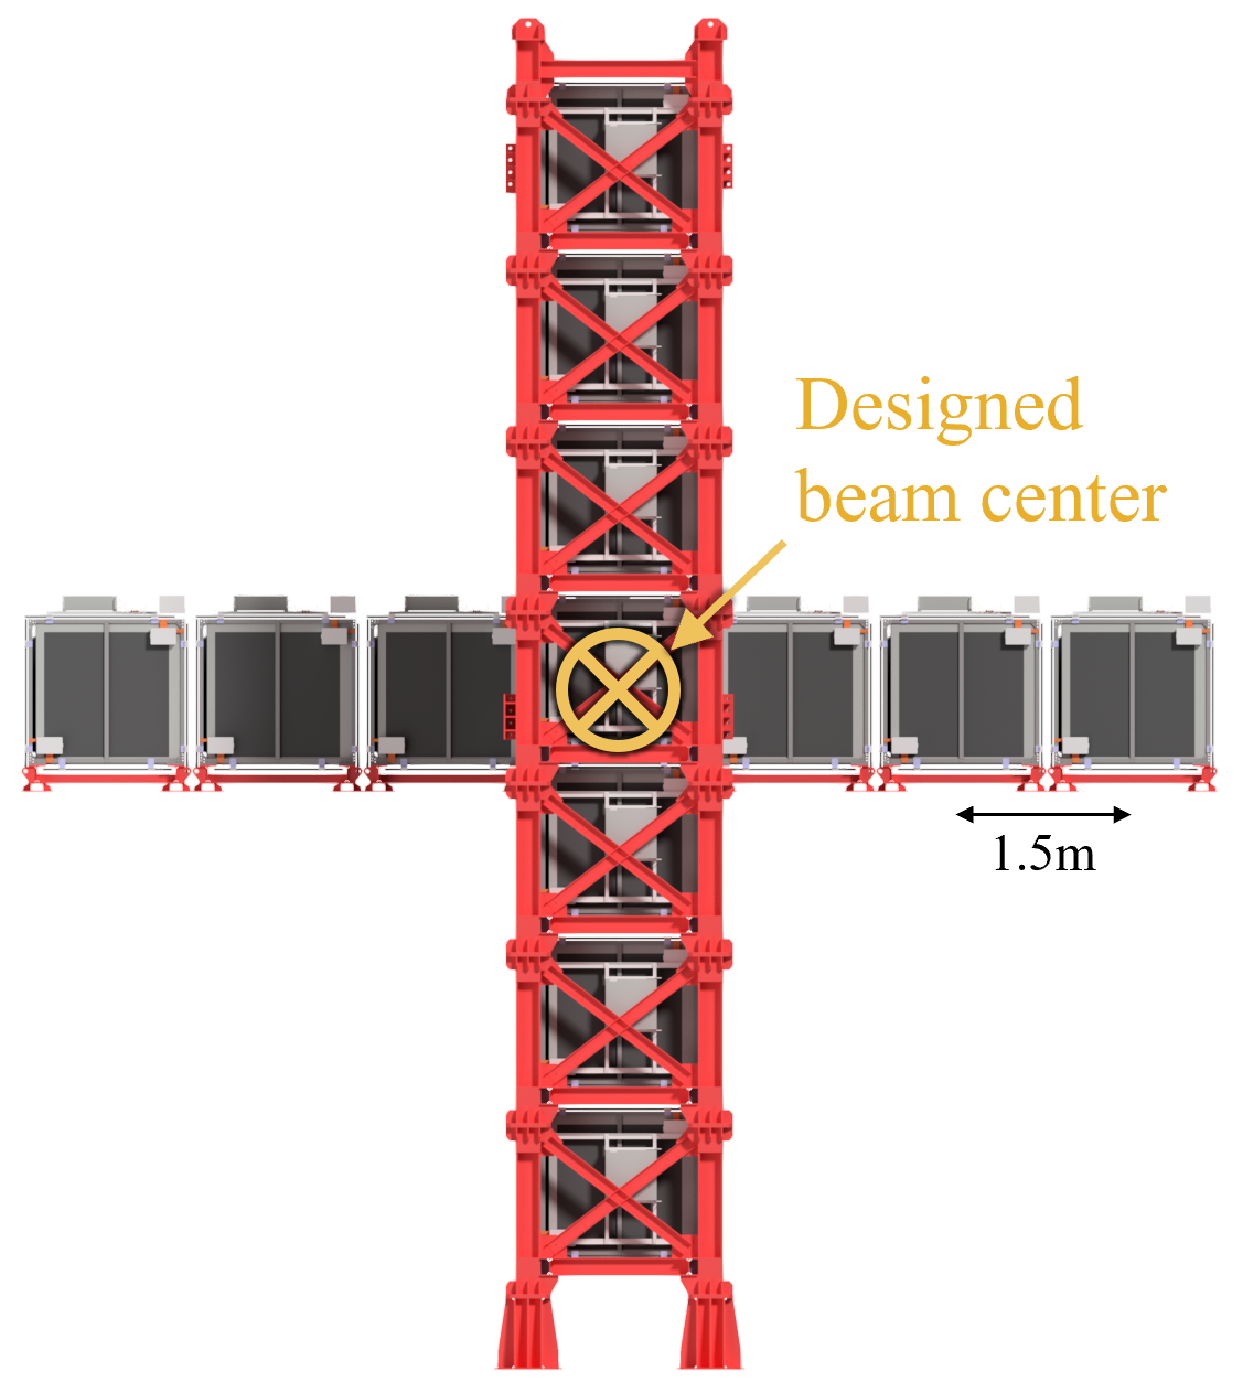
\includegraphics[width=\textwidth, trim={0mm 0mm 0mm 0mm}, clip,page=1]{Figures/Detectors/T2KINGRIDDiagram.pdf}
  \end{subfigure}%
  \begin{subfigure}[t]{0.55\textwidth}
    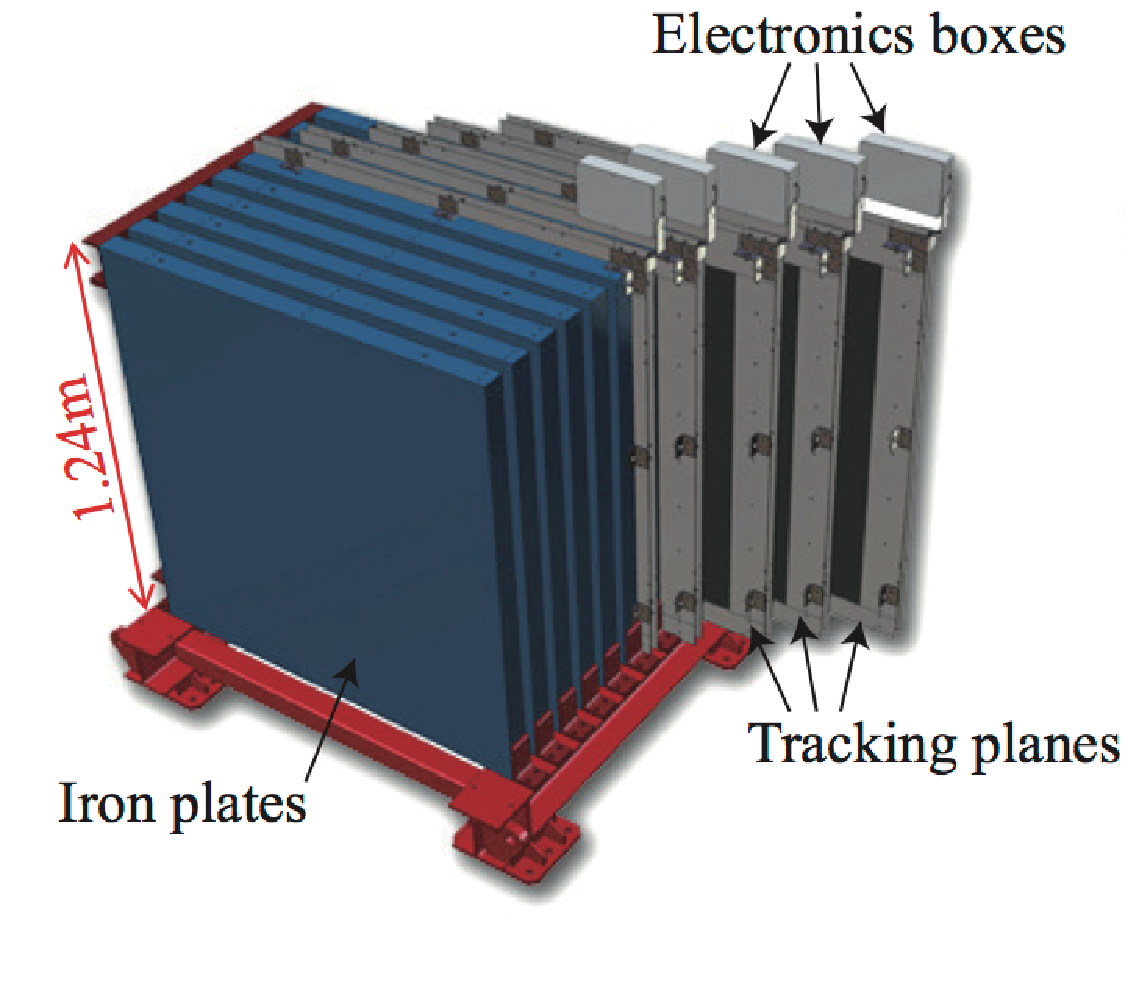
\includegraphics[width=\textwidth, trim={0mm 0mm 0mm 0mm}, clip,page=1]{Figures/Detectors/T2KINGRIDModule.pdf}
  \end{subfigure}%
  \caption{Left panel: The Interactive Neutrino GRID on-axis Detector. 14 modules are arranged in a cross-shape configuration, with the centre modules being directly aligned with the on-axis beam. Right panel: The layout of a single module of the INGRID detector. Both figures are recreated from \cite{t2k_det}.}
  \label{fig:T2KSKExp_T2K_INGRID}
\end{figure}

The INGRID detector can measure the beam direction to an uncertainty of \quickmath{0.4\text{mrad}} and the beam centre within a resolution of \quickmath{10 \text{cm}} \cite{t2k_det}. The beam direction in both the vertical and horizontal directions is discussed in \cite{Suzuki_2015} and it is found to be in good agreement with the MUMON monitor described in \autoref{subsec:T2KSKExp_T2K_NeutrinoBeam}.


\chapter{Bayesian Statistics and Markov Chain Monte Carlo Techniques}
\label{chap:MarkovChainMonteCarlo}
This thesis presents a Bayesian oscillation analysis. To extract the oscillation parameters, a Markov Chain Monte Carlo (MCMC) method is used. This chapter explains the theory of how parameter estimates can be determined using this technique and condenses the material found in the literature \cite{mcmc_handbook, mcmc_practice, thesis_clarence, thesis_kirsty}.

The oscillation parameter determination presented here is built upon a simultaneous fit to neutrino beam data in the near detector, beam data at SK, and atmospheric data at SK. In total, there are four oscillation parameters of interest (\quickmath{\sin^{2}(\theta_{23})}, \quickmath{\sin^{2}(\theta_{13})}, \quickmath{\Delta m^{2}_{32}}, and \quickmath{\delta_{CP}}), two oscillation parameters to which this study will not be sensitive (\quickmath{\sin^{2}(\theta_{12})}, \quickmath{\Delta m^{2}_{21}}) and  many nuisance parameters that control the systematic uncertainty models.
%The systematic uncertainties can be grouped into categories depending on how they are defined: $574$ bin-normalisations due to the near detector response, $45$ bin-normalisations to describe the far detector response to neutrino beam events, $27$ parameters to describe the detector response to atmospheric neutrino events, $100$ to model the bin-normalisation due to beam flux uncertainties, $18$ which model the atmospheric flux uncertainties, and $87$ to describe the correlated cross-section model. An alternative parameterisation, where the far detector response is correlated between the beam and atmospheric samples, replaces the bin-normalisation parameters with $224$ shift and smear systematics. Section Link to Systematics Chapter describes the systematic model in more depth.

This analysis uses a Monte Carlo technique to generate a multi-dimensional probability distribution across all of the model parameters used in the fit. To determine an estimate for each parameter, this multi-dimensional object is integrated over all other parameters. This process is called Marginalisation and is described in \autoref{sec:MarkovChainMonteCarlo_Marginalisation}. Monte Carlo techniques approximate the probability distribution of each parameter within the limit of generating infinite samples. As ever, generating a large number of samples is time and resource-dependent. Therefore, an MCMC technique is utilised within this analysis to reduce the required number of steps to sufficiently sample the parameter space. This technique is described in further detail in \autoref{sec:MarkovChainMonteCarlo_MarkovChainMC}.

\finish{Introduce MaCh3 and say what I did on it}

\section{Bayesian Statistics}
\label{sec:MarkovChainMonteCarlo_BayesianStatistics}

Bayesian inference treats observable data, \quickmath{D}, and model parameters, \quickmath{\vec{\theta}}, on equal footing such that a probability model of both data and parameters is required. This is the joint probability distribution \quickmath{P(D, \vec{\theta})} and can be described by the prior distribution for model parameters \quickmath{P(\vec{\theta})} and the likelihood of the data given the model parameters \quickmath{P(D|\vec{\theta})},

\begin{equation}
  P(D,\vec{\theta}) = P(D|\vec{\theta})P(\vec{\theta}).
\end{equation}

The prior distribution, \quickmath{P(\vec{\theta})}, describes all previous knowledge about the parameters within the model. For example, if the risk of developing health problems is known to increase with age, the prior distribution would describe the increase. For the purpose of this analysis, the prior distribution is typically the best-fit values taken from external data measurements with a Gaussian uncertainty. The prior distribution can also contain correlations between model parameters. In an analysis using Monte Carlo techniques, the likelihood of measuring some data assuming some set of model parameters is calculated by comparing the Monte Carlo prediction generated at that particular set of model parameters to the data.

It is parameter estimation that is important for this analysis and as such, we apply Bayes' theorem \cite{Bayes:1764vd} to calculate the probability for each parameter to have a certain value given the observed data, \quickmath{P(\vec{\theta}|D)}, which is known as the posterior distribution (often termed the posterior). This can be expressed as

\begin{equation}
  \label{eq:MarkovChainMonteCarlo_PosteriorDistribution}
  P(\vec{\theta}|D) = \frac{ P(D|\vec{\theta}) P(\vec{\theta}) }{\int P(D|\vec{\theta}) P(\vec{\theta}) d\vec{\theta}}.
\end{equation}

The denominator in \autoref{eq:MarkovChainMonteCarlo_PosteriorDistribution} is the integral of the joint probability distribution over all values of all parameters used within the fit. For brevity, we say that the posterior distribution is

\begin{equation}
  \label{eq:MarkovChainMonteCarlo_PosteriorDistributionReduced}
  P(\vec{\theta}|D) \propto P(D|\vec{\theta}) P(\vec{\theta}).
\end{equation}

%In \autoref{sec:MarkovChainMonteCarlo_Marginalisation}, we see that for the cases used within this analysis, it is reasonable to know the posterior to some normalisation constant.
For the purposes of this analysis, it is acceptable to neglect the normalisation term and focus on this proportional relationship.

\subsection{Application of Prior Knowledge}
\label{sec:MarkovChainMonteCarlo_Priors}

The posterior distribution is proportional to the prior uncertainty applied to each parameter, as illustrated by \autoref{eq:MarkovChainMonteCarlo_PosteriorDistributionReduced}. This means that it is possible to change the prior after the posterior distribution has been determined. The prior uncertainty of a particular parameter can be `divided' out of the posterior distribution and the resulting distribution can be reweighted using the new prior uncertainty that is to be applied. The methodology and implementation of changing the prior follows that described in \cite{thesis_artur}. 

An example implementation that is useful for this analysis is the application of the ``reactor constraint''. As discussed in \autoref{sec:Theory_Summary}, an external constraint on \quickmath{\sin^{2}(\theta_{13})} is determined from measurements taken from reactor experiments. However, the sensitivities from just using the T2K and SK samples is equally as important. Without this technique, two fits would have to be run, doubling the required resources. Therefore, the key benefit for this analysis is the fact that only a single `fit' has to be performed and can be used to build the two posterior distributions of the with and without reactor constraint applied.

\section{Monte Carlo Simulation}
\label{sec:MarkovChainMonteCarlo_MonteCarloSimulation}
Monte Carlo techniques are used to numerically solve a complex problem that does not necessarily have an analytical solution. These techniques rely on building a large ensemble of samples from an unknown distribution and then using the ensemble to approximate the properties of the distribution.

An example that uses Monte Carlo techniques is to calculate the area underneath a curve. For example, take the problem of calculating the area under a straight line with gradient \quickmath{M = 0.4} and intercept \quickmath{C = 1.0}. Analytically, one can calculate the area under the line is equal to 30 units for \quickmath{0 \leq x \leq 10}. Using Monte Carlo techniques, one can calculate the area under this line by throwing many random values for the \quickmath{x} and \quickmath{y} components of each sample and then calculating whether that point falls below the line. The area can then be calculated by the ratio of points below the line to the total number of samples thrown multiplied by the total area in which samples were scattered. The study is shown in \autoref{fig:MCMC_MCTechnique} highlights this technique and finds the area under the curve to be \quickmath{29.9} compared to an analytical solution of \quickmath{30.0}. The deviation of the numerical to analytical solution can be attributed to the number of samples used in the study. The accuracy of the approximation in which the properties of the Monte Carlo samples replicate those of the desired distribution is dependent on the number of samples used. Replicating this study with a differing number of Monte Carlo samples used in each study (As shown in \autoref{fig:MCMC_MCTechniqueNThrowsStudy}) highlights how the Monte Carlo techniques are only accurate within the limit of a high number of samples.

Whilst the above example has an analytical solution, these techniques are just as applicable to complex solutions. Clearly,  any numerical solution is only as useful as its efficiency. As discussed, the accuracy of the Monte Carlo technique is dependent upon the number of samples generated to approximate the properties of the distribution. Furthermore, if the positions at which the samples are evaluated are not `cleverly' picked, the efficiency of the Monte Carlo technique significantly drops. Given the example in \autoref{fig:MCMC_MCTechnique}, if the region in which the samples are scattered significantly extends passed the region of interest, many calculations will be calculated but do not add to the ability of the Monte Carlo technique to achieve the correct result. For instance, any sample evaluated at a \quickmath{y \geq 5} could be removed without affecting the final result. This does bring in an aspect of the `chicken and egg' problem in that to achieve efficient sampling, one needs to know the distribution beforehand.

\begin{figure}[h]
  \begin{subfigure}[t]{0.80\textwidth}
    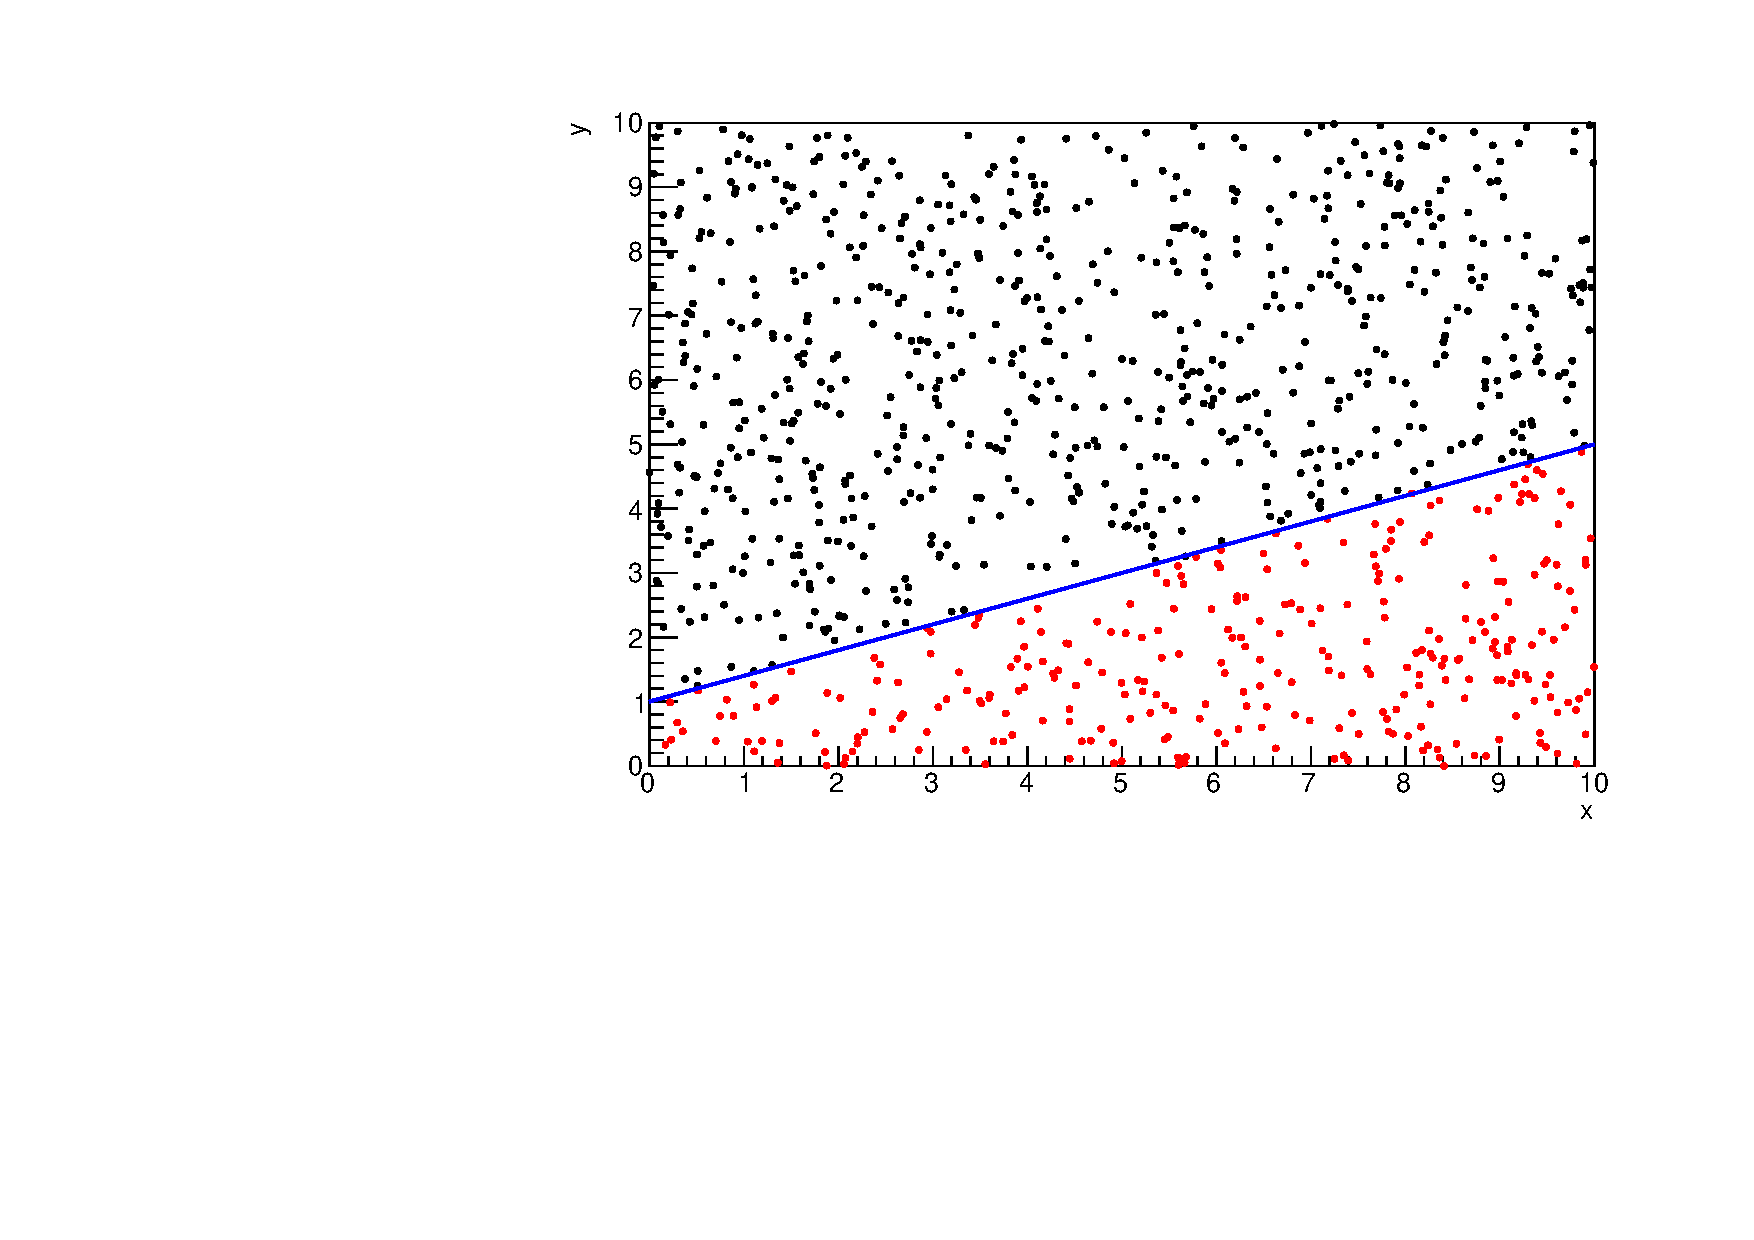
\includegraphics[width=\textwidth, trim={0mm 0mm 0mm 0mm}, clip,page=1]{Figures/MCMC/MCTechnique.pdf}
  \end{subfigure}
  \caption{Example of using Monte Carlo techniques to find the area under the blue line. The gradient and intercept of the line are \quickmath{0.4} and \quickmath{1.0} respectively. The area found to be under the curve using one thousand samples is \quickmath{29.9} units.}
  \label{fig:MCMC_MCTechnique}
\end{figure}

\begin{figure}[h]
  \begin{subfigure}[t]{0.80\textwidth}
    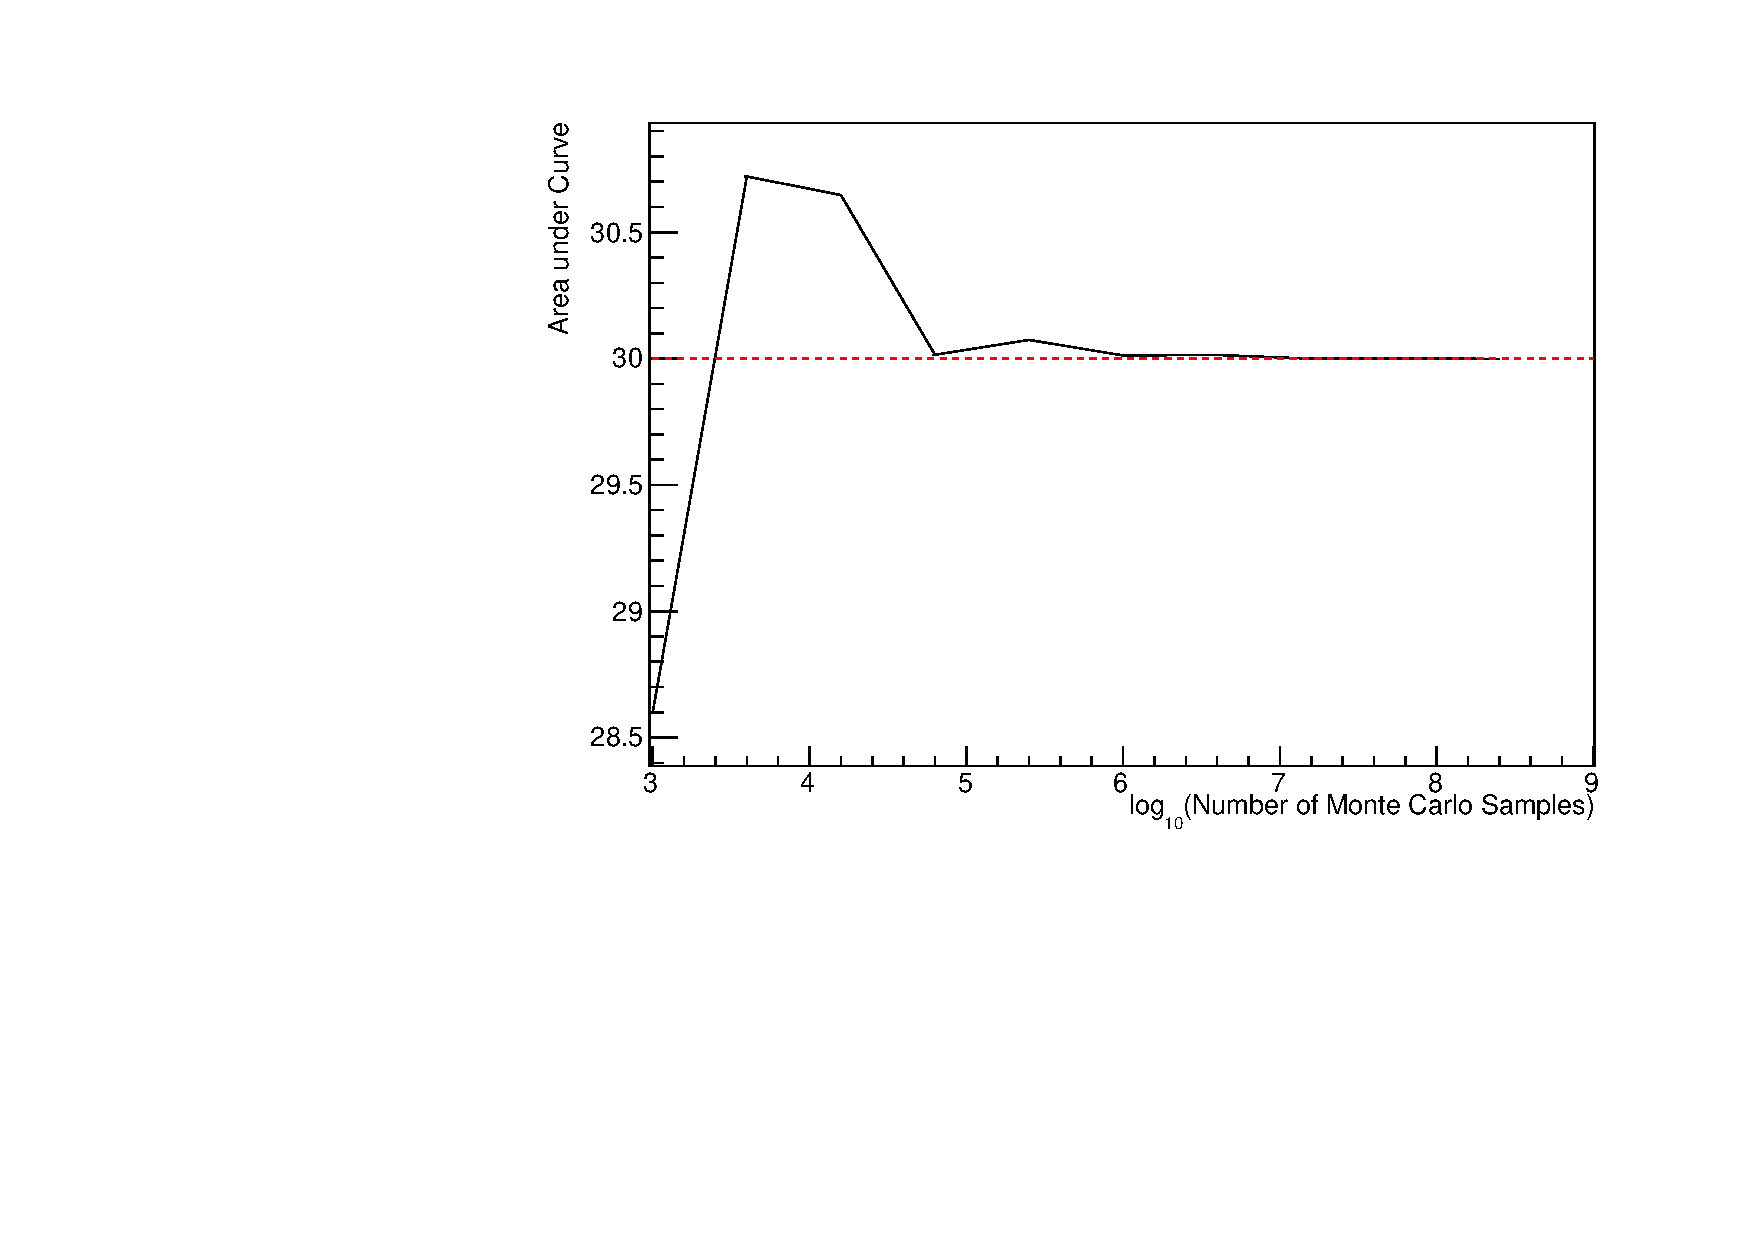
\includegraphics[width=\textwidth, trim={0mm 0mm 0mm 0mm}, clip,page=1]{Figures/MCMC/MCTechnique_NThrowsStudy.pdf}
  \end{subfigure}
  \caption{The area under a line of gradient \quickmath{0.4} and intercept \quickmath{1.0} for the range \quickmath{0 \leq x \leq 10} as calculated using Monte Carlo techniques as a function of the number of samples used in each repetition. The analytical solution to the area is 30 units as given by the red line.}
  \label{fig:MCMC_MCTechniqueNThrowsStudy}
\end{figure}

\subsection{Markov Chain Monte Carlo}
\label{sec:MarkovChainMonteCarlo_MarkovChainMC}
This analysis utilises a multi-dimensional probability distribution, with some dimensions being significantly more constrained than others. These constraints can be from prior knowledge of parameter distributions from external data or un-physical regions in which parameters can not exist. To maximise the efficiency of building the posterior distribution, a Markov Chain Monte Carlo (MCMC) technique is used. This employs a Markov chain to select the points at which to sample the posterior distribution. It performs a semi-random stochastic walk through the allowable parameter space. This builds a posterior distribution which has the property that the density of sampled points is proportional to the probability density of that parameter. This means that the samples produced by this technique are not statistically independent but they will cover the space of the distribution.

A Markov chain functions by selecting the position of step \quickmath{\vec{x}_{i+1}} based on the position of \quickmath{\vec{x}_{i}}. The space in which the Markov chain selects samples is dependent upon the total number of parameters utilised within the fit, where a discrete point in this space is described by the N-dimensional space \quickmath{\vec{x}}. In a perfectly operating Markov chain, the position of the next step depends solely on the previous step and not on the further history of the chain (\quickmath{\vec{x}_{0}}, \quickmath{\vec{x}_{1}}, etc.). However, in solving the multi-dimensionality of the fit used within this analysis, each step becomes correlated with several of the steps preceding itself.
%This behaviour is further explained in \autoref{sec:MarkovChainMonteCarlo_MCMCOptimisation}.
Providing the MCMC chain is well optimised, it will begin to converge towards a unique stationary distribution. The period between the chain's initial starting point and the convergence to the unique stationary distribution is colloquially known as the burn-in period.
%This is discussed further in \autoref{sec:MarkovChainMonteCarlo_MCMCOptimisation}.
Once the chain reaches the stationary distribution, all points sampled after that point will look like samples from that distribution.

Further details of the theories underpinning MCMC techniques are discussed in \cite{mcmc_practice} but can be summarised by the requirement that the chain satisfies the three `regularity conditions':

\begin{itemize}
\item Irreducibility: From every position in the parameter space \quickmath{\vec{x}}, there must exist a non-zero probability for every other position in the parameter space to be reached.
\item Recurrence: Once the chain arrives at the stationary distribution, every step following from that position must be samples from the same stationary distribution.
\item Aperiodicity: The chain must not repeat the same sequence of steps at any point throughout the sampling period.
\end{itemize}

The output of the chain after burn-in (i.e. the sampled points after the chain has reached the stationary distribution) can be used to approximate the posterior distribution and model parameters \quickmath{\vec{\theta}}. To achieve the requirement that the unique stationary distribution found by the chain be the posterior distribution, one can use the Metropolis-Hastings algorithm. This guides the stochastic process depending on the likelihood of the current proposed step compared to that of the previous step. %Implementation and other details of this technique are discussed in \autoref{sec:MarkovChainMonteCarlo_MetropoliseHastingsAlgorithm}.

\subsection{Metropolis-Hastings Algorithm}
\label{sec:MarkovChainMonteCarlo_MetropoliseHastingsAlgorithm}

As a requirement for MCMCs, the Markov chain implemented in this technique must have a unique stationary distribution that is equivalent to the posterior distribution. To ensure this requirement and that the regularity conditions are met, this analysis utilises the Metropolis-Hastings (MH) algorithm \cite{metropolis, hastings}. For the \quickmath{i^{th}} step in the chain, the MH algorithm determines the position in the parameter space to which the chain moves to based on the current step, \quickmath{\vec{x}_{i}}, and the proposed step, \quickmath{\vec{y}_{i+1}}. The proposed step is randomly selected from some proposal function \quickmath{f(\vec{x}_{i+1}|\vec{x}_{i})}, which depends solely on the current step (ie. not the further history of the chain). The next step in the chain \quickmath{\vec{x}_{i+1}} can be either the current step or the proposed step determined by whether the proposed step is accepted or rejected. To decide if the proposed step is selected, the acceptance probability, \quickmath{\alpha(\vec{x}_{i},\vec{y}_{i})}, is calculated as

\begin{equation}
  \label{eq:MarkovChainMonteCarlo_FullAcceptanceProbability}
  \alpha(\vec{x}_{i},\vec{y}_{i+1}) = \min\left(1,\frac{P(\vec{y}_{i+1}|D)f(\vec{x}_{i}|\vec{y}_{i+1})}{P(\vec{x}_{i}|D)f(\vec{y}_{i+1}|\vec{x}_{i})} \right).
\end{equation}

Where \quickmath{P(\vec{y}_{i+1}|D)} is the posterior distribution as introduced in \autoref{sec:MarkovChainMonteCarlo_BayesianStatistics}. To simplify this calculation, the proposal function is required to be symmetric such that \quickmath{f(\vec{x}_{i}|\vec{y}_{i+1}) = f(\vec{y}_{i+1}|\vec{x}_{i})}. In practice, a multi-variate Gaussian distribution is used to throw parameter proposals. This reduces \autoref{eq:MarkovChainMonteCarlo_FullAcceptanceProbability} to

\begin{equation}
  \label{eq:MarkovChainMonteCarlo_ReducedAcceptanceProbability}
  \alpha(\vec{x}_{i},\vec{y}_{i+1}) = \min\left(1,\frac{P(\vec{y}_{i+1}|D)}{P(\vec{x}_{i}|D)} \right).
\end{equation}

\finish{Figure out what Giles means}

After calculating this quantity, a random number, \quickmath{\beta}, is generated uniformly between 0 and 1. If \quickmath{\beta \leq \alpha(\vec{x}_{i},\vec{y}_{i+1})}, the proposed step is accepted. Otherwise, the chain sets the next step equal to the current step. This procedure is repeated for subsequent steps. This can be interpreted as if the posterior probability of the proposed step is greater than that of the current step, (\quickmath{P(\vec{y}_{i+1}|D) \geq P(\vec{x}_{i}|D)}), the proposed step will always be accepted. If the opposite is true, (\quickmath{P(\vec{y}_{i+1}|D) \leq P(\vec{x}_{i}|D)}), the proposed step will be accepted with probability \quickmath{P(\vec{x}_{i}|D) / P(\vec{y}_{i+1}|D)}. This ensures that the Markov chain does not get trapped in any local minima in the potentially non-Gaussian posterior distribution. The outcome of this technique is that the density of steps taken in a discrete region is directly proportional to the probability density in that region.

\subsection{MCMC Optimisation}
\label{sec:MarkovChainMonteCarlo_MCMCOptimisation}
As discussed in \autoref{sec:MarkovChainMonteCarlo_MetropoliseHastingsAlgorithm}, the proposal function invoked within the MH algorithm can take any form and the chain will still converge to the stationary distribution. At each set of proposed parameter values, a prediction of the same spectra has to be generated which requires significant computational resources. Therefore, the number of steps taken before the unique stationary distribution is found should be minimised as only steps after convergence add information to the oscillation analysis. Furthermore, the chain should entirely cover the allowable parameter space to ensure that all values have been considered. Tuning the distance that the proposal function jumps between steps on a parameter-by-parameter basis can both minimise the length of the burn-in period and ensure that the correlation between step \quickmath{\vec{x}_{i}} and \quickmath{\vec{x}_{j}} is sufficiently small.

The effect of changing the width of the proposal function is highlighted in \autoref{fig:MCMC_MCTechniqueStepSizeStudy}. Three scenarios, each with the same underlying stationary distribution (A Gaussian of width \quickmath{1.0} and mean \quickmath{0.}), are presented. The only difference between the three scenarios is the width of the proposal function, colloquially known as the `step size \quickmath{\sigma}'. Each scenario starts at an initial parameter value of \quickmath{10.0} which would be considered an extreme variation. For the case where \quickmath{\sigma = 0.1}, it is clear to see that the chain takes a long time to reach the expected region of the parameter. This indicates that this chain would have a large burn-in period and does not converge to the stationary distribution until step \quickmath{\sim 500}. Furthermore, whilst the chain does move towards the expected region, each step is significantly correlated with the previous. Considering the case where \quickmath{\sigma = 5.0}, the chain approaches the expected parameter region almost instantly meaning that the burn-in period is not significant. However, there are clearly large regions of steps where the chain does not move. This is likely due to the chain proposing steps in the tails of the distribution which have a low probability of being accepted. Consequently, this chain would take a significant number of steps to fully span the allowable parameter region. For the final scenario, where \quickmath{\sigma = 0.5}, you can see a relatively small burn-in period of approximately \quickmath{100} steps. Once the chain reaches the stationary distribution, it moves throughout the expected region of parameter values many times, sufficiently sampling the full parameter region. This example is a single parameter varying across a continuous distribution and does not fully reflect the difficulties in the many-hundred multi-variate parameter distribution used within this analysis. However, it does give a conceptual idea of the importance of selecting the proposal function and associated step size. 

\begin{figure}[h]
  \begin{subfigure}[t]{\textwidth}
    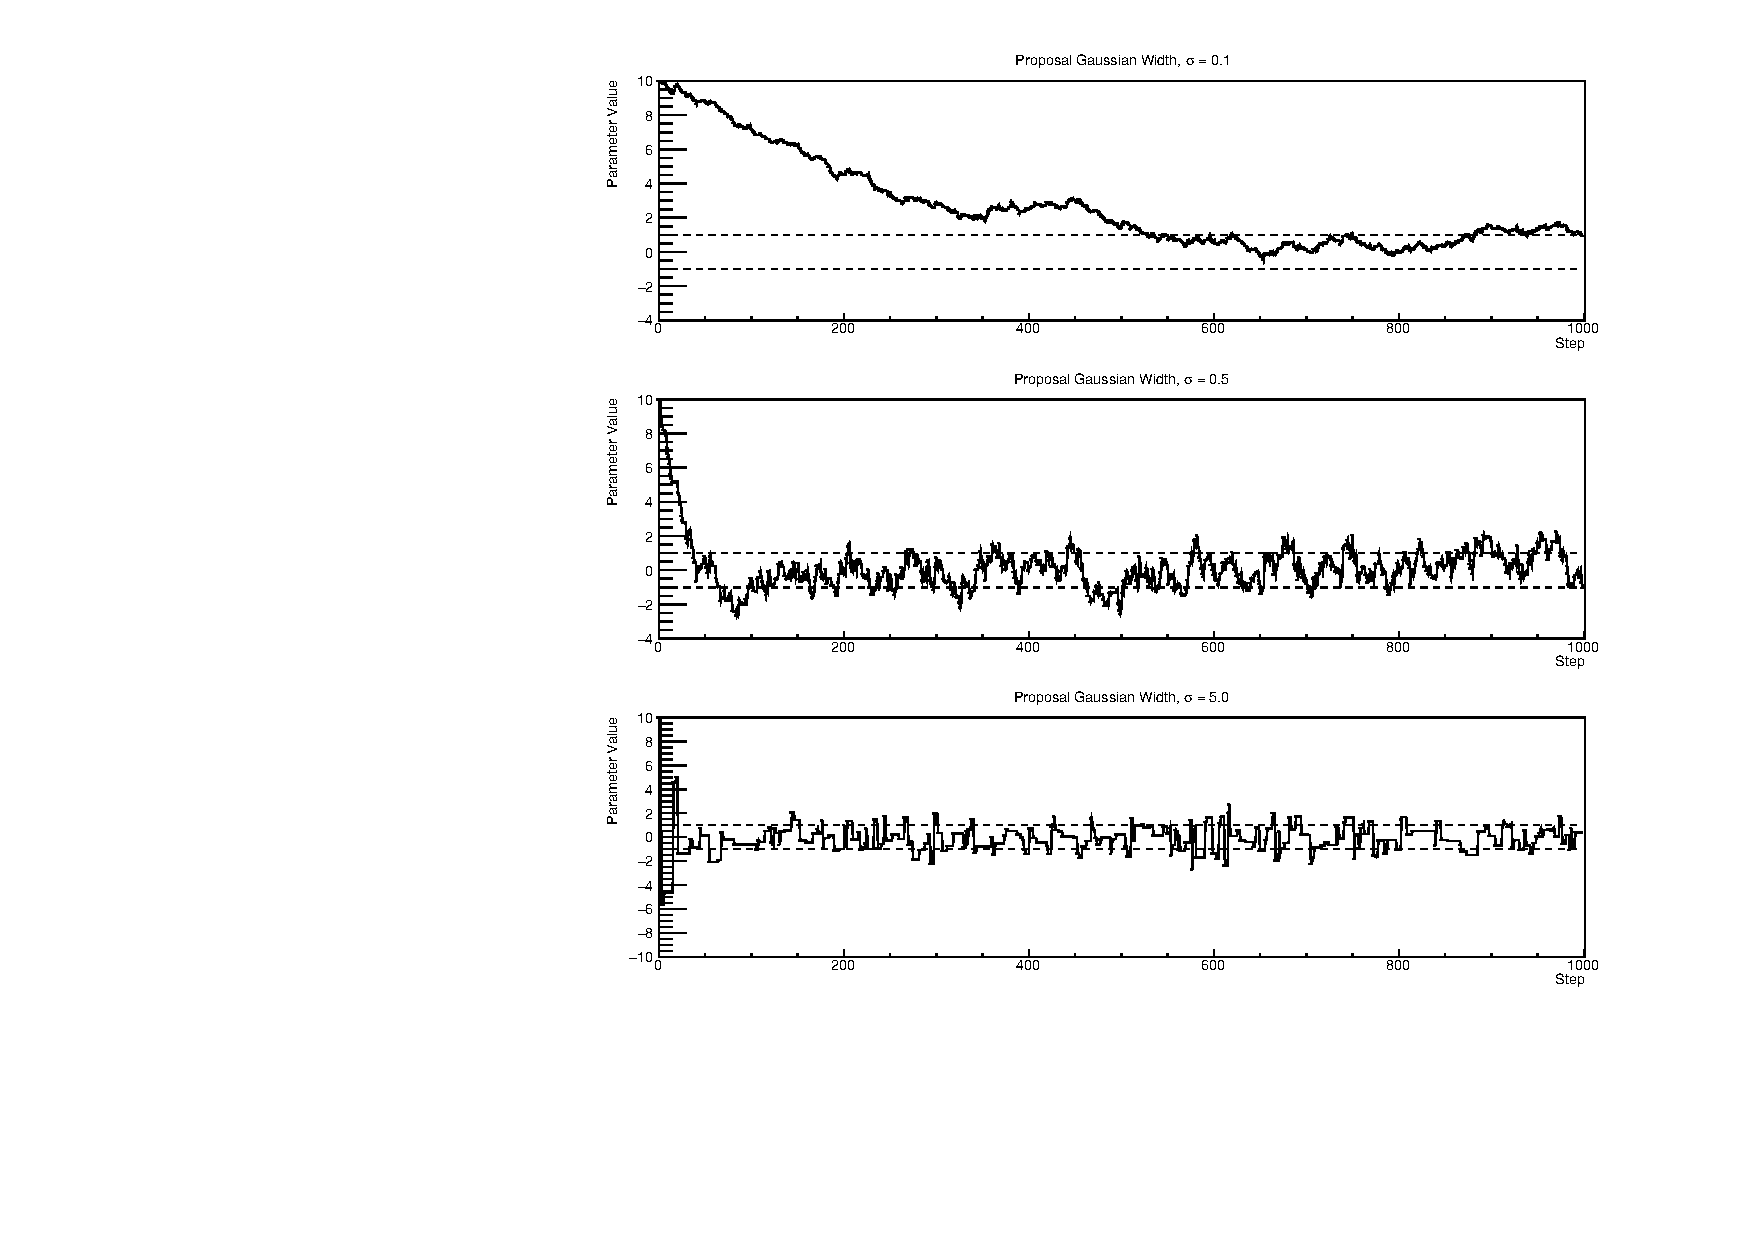
\includegraphics[width=\textwidth, trim={10mm 0mm 18mm 0mm}, clip,page=1]{Figures/MCMC/MCMCTechnique_StepSizes.pdf}
  \end{subfigure}
  \caption{Three MCMC chains, each with a stationary distribution equal to a Gaussian centered at \quickmath{0} and width \quickmath{1} (As indicated by the black dotted lines). All of the chains use a Gaussian proposal function but have different widths (or `step size \quickmath{\sigma}'). The top panel has \quickmath{\sigma = 0.1}, middle panel has \quickmath{\sigma = 0.5} and the bottom panel has \quickmath{\sigma = 5.0}.}
  \label{fig:MCMC_MCTechniqueStepSizeStudy}
\end{figure}

As discussed, step size tuning directly correlates to the average step acceptance rate. If the step size is too small, many steps will be accepted but the chain moves slowly. If the opposite is true, many steps will be rejected as the chain proposes steps in the tails of the distribution. Discussion in \cite{Dunkley2005-xz} suggests that the `ideal' acceptance rate of a high dimension MCMC chain should be approximately \quickmath{\sim 25\%}. An ``ideal'' step size \cite{Dunkley2005-xz} of

\begin{equation}
  \label{eq:MCMC_IdealStepSize}
  \sigma = \frac{2.4}{N_{p}},
\end{equation}

where \quickmath{N_{p}} is the number of parameters included in the MCMC fit. However, the complex correlations between systematics mean that some parameters have to be hand-tuned and many efforts have been taken to select a set of parameter-by-parameter step sizes to approximately reach the ideal acceptance rate.

\autoref{fig:MCMC_MCTechniqueLLHVsStep} highlights the likelihood as calculated by the fit in \finish{Link to AsimovA Sensitivity Section} as a function of the number of steps in each chain. In practice, many independent MCMC chains are run simultaneously to parallelise the task of performing the fit. This figure overlays the distribution found in each chain. As seen, the likelihood decreases from its initial value and converges towards a stationary distribution after \quickmath{\sim 1 \times 10^{5}} steps.

\begin{figure}[h]
  \begin{subfigure}[t]{0.8\textwidth}
    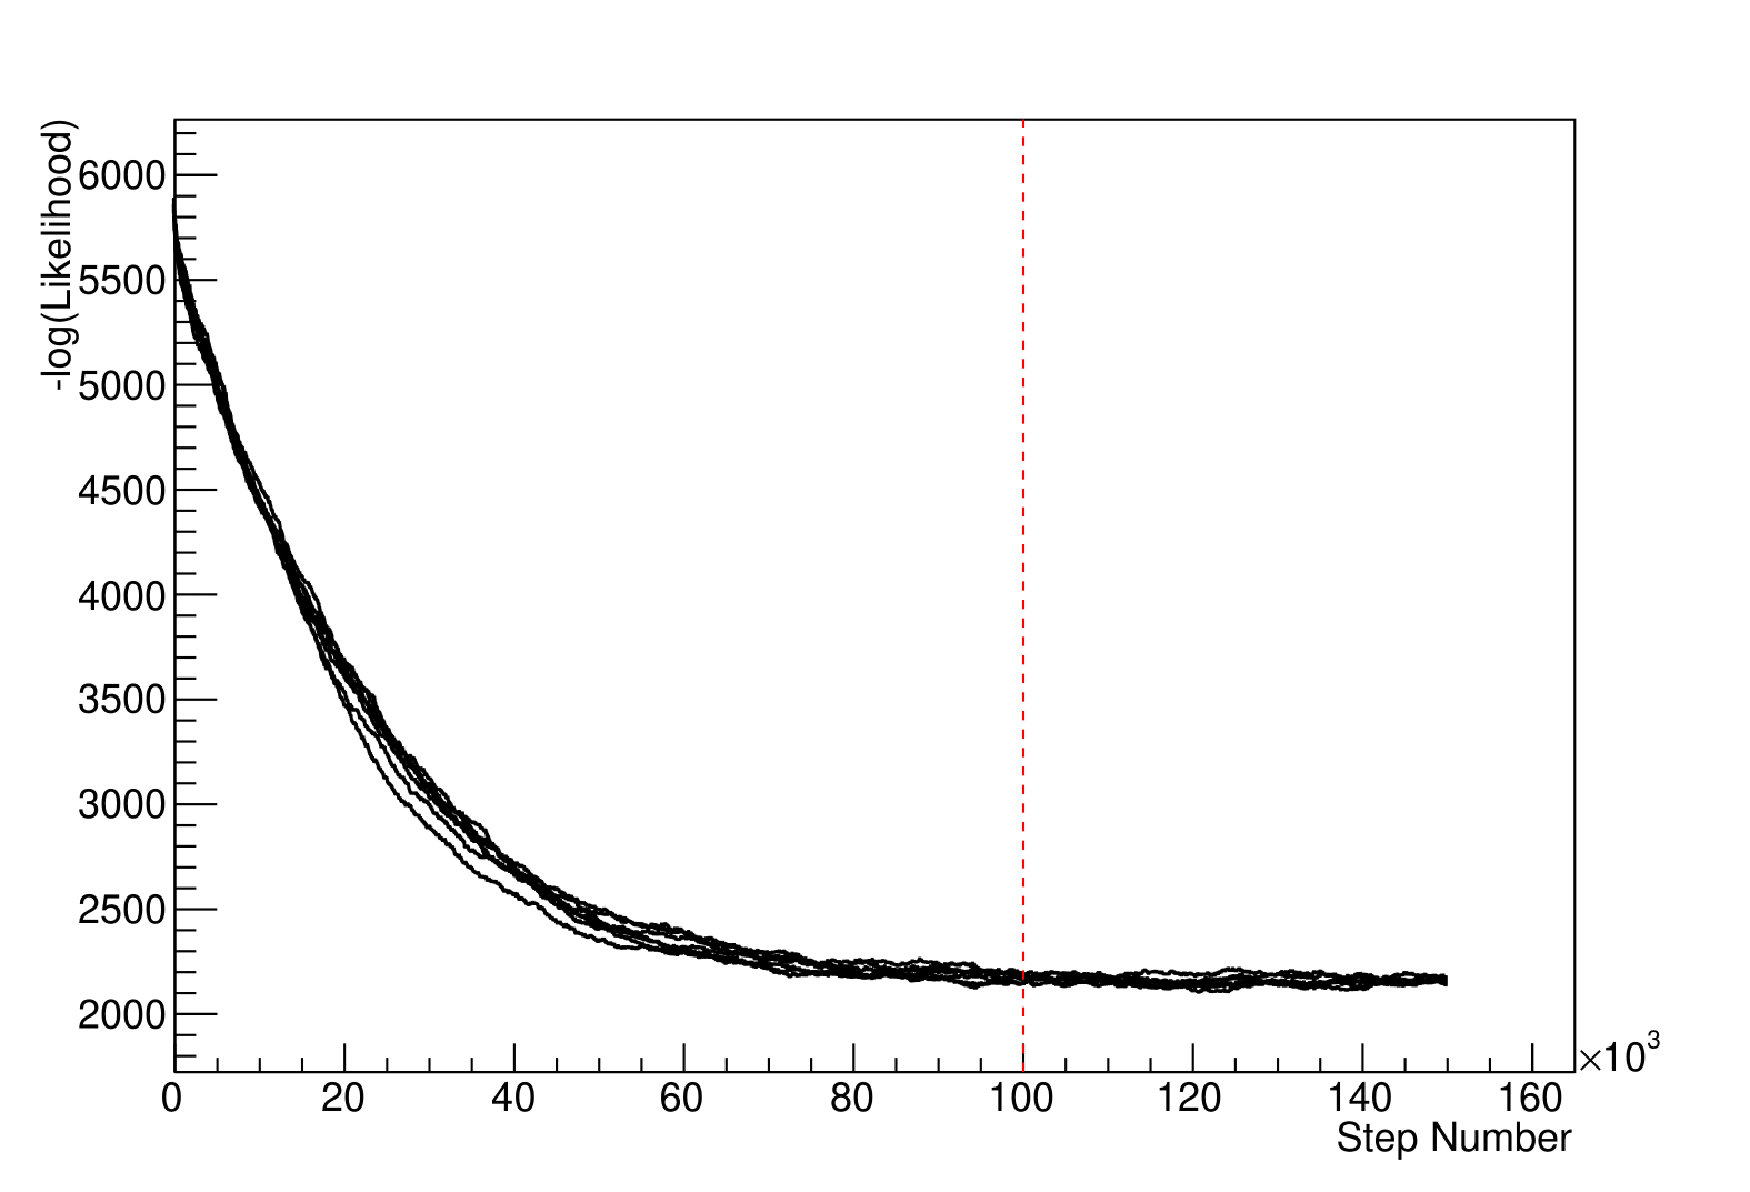
\includegraphics[width=\textwidth, trim={0mm 0mm 0mm 0mm}, clip,page=1]{Figures/MCMC/MCTechnique_LLHStep.pdf}
  \end{subfigure}
  \caption{The log-likelihood from the fit detailed in \finish{Link to AsimovA Sensitivity Section} as a function of the number of steps accumulated in each fit. Many independent MCMC chains were run in parallel and overlaid on this plot. The red line indicates the \quickmath{1 \times 10^{5}} step burn-in period after which the log-likelihood becomes stable.}
  \label{fig:MCMC_MCTechniqueLLHVsStep}
\end{figure}

Multiple configurations of this analysis have been performed throughout this thesis where different samples or systematics have been used. For all of these configurations, it was found that a burnin period of \quickmath{1 \times 10^{5}} was sufficient in all cases.

\section{Understanding the MCMC Results}
\label{sec:MarkovChainMonteCarlo_UnderstandingMCMCResults}

The previous sections have described how to generate the posterior probability distribution using Bayesian MCMC techniques. However, this analysis focuses on oscillation parameter determination. The posterior distribution output from the chain is a high-dimension object, with as many dimensions as there are parameters included in the oscillation analysis. However, this multi-dimensional object is difficult to conceptualize so parameter estimations are often presented in one or two-dimensional projections of this probability distribution. To do this, we invoke the marginalisation technique highlighted in \autoref{sec:MarkovChainMonteCarlo_Marginalisation}.

\subsection{Marginalisation}
\label{sec:MarkovChainMonteCarlo_Marginalisation}

The output of the MCMC chain is a highly dimensional probability distribution which is very difficult to interpret. From the standpoint of an oscillation analysis experiment, the one or two-dimensional `projections' of the oscillation parameters of interest are most relevant. Despite this, the best fit values and uncertainties on the oscillation parameters of interest should correctly encapsulate the correlations to the other systematic uncertainties (colloquially called `nuisance' parameters). For this joint beam and atmospheric analysis, the oscillation parameters of interest are \quickmath{\sin^{2}(\theta_{23})}, \quickmath{\sin^{2}(\theta_{13})}, \quickmath{\Delta m^{2}_{32}}, and\quickmath{\delta_{CP}}. All other parameters (including the oscillation parameters this fit is insensitive to) are deemed nuisance parameters. To generate these projections, we rely upon integrating the posterior distribution over all nuisance parameters. This is called marginalisation. This technique also explains why it is acceptable to neglect the normalisation constant of the posterior distribution, which was discussed in \autoref{sec:MarkovChainMonteCarlo_BayesianStatistics}.

A simple example of the marginalisation technique is to imagine the scenario where two coins are flipped. To determine the probability that the first coin returned a `head', the exact result of the second coin flip is disregarded and simply integrated over. For the parameters of interest, \quickmath{\vec{\theta}_{i}}, we can calculate the marginalised posterior by integrating over the nuisance parameters, \quickmath{\vec{\theta}_{n}}. In this case, \autoref{eq:MarkovChainMonteCarlo_PosteriorDistribution} becomes

\begin{equation}
P(\vec{\theta}_{i}|D) = \frac{\int P(D|\vec{\theta}_{i},\vec{\theta}_{n}) P(\vec{\theta}_{i},\vec{\theta}_{n}) d\vec{\theta}_{n}}{\int P(D|\vec{\theta}) P(\vec{\theta}) d\vec{\theta}}
\end{equation}

Where \quickmath{P(\vec{\theta}_{i},\vec{\theta}_{n})} encodes the prior knowledge about the uncertainty and correlations between the parameters of interest and the nuisance parameters. In practice, this is simply taking the one or two-dimensional projection of the multi-dimensional probability distribution.

While in principle an easy solution to a complex problem, correlations between the interesting and nuisance parameters can bias the marginalised results. A similar effect is found when the parameters being marginalised over have non-Gaussian probability distributions. For example, \autoref{fig:MCMC_MCTechniqueMarginalisationProblems} highlights the marginalisation bias in the probability distribution found for a parameter when requiring a correlated parameter to have a positive parameter value. Due to the complex nature of the oscillation parameter fit presented in this thesis, there are correlations occurring between the oscillation parameters of interest and the other nuisance parameters included in the fit.

\begin{figure}[h]
  \begin{subfigure}[t]{0.48\textwidth}
    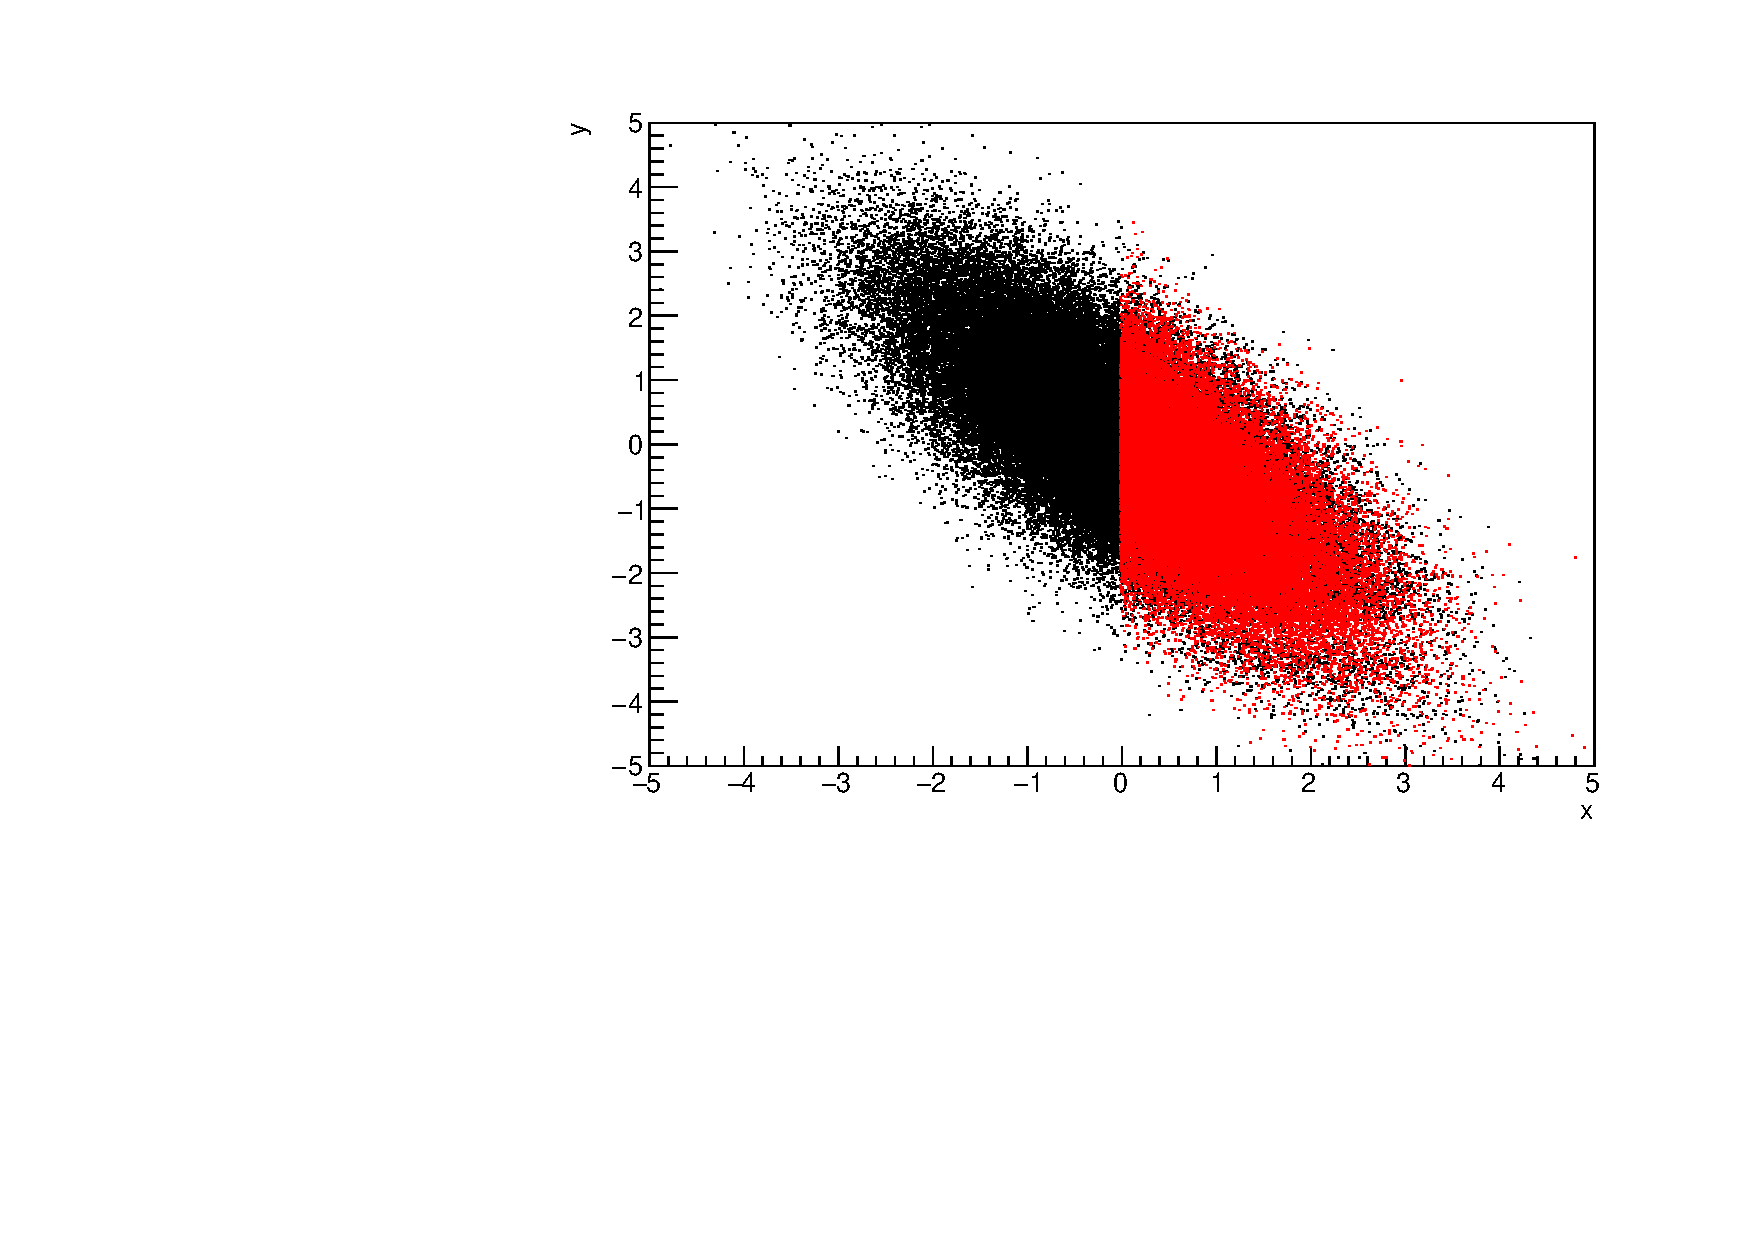
\includegraphics[width=\textwidth, trim={0mm 0mm 0mm 0mm}, clip,page=1]{Figures/MCMC/MCTechnique_Marginalisation2D_Double_Correlations.pdf}
  \end{subfigure} %
    \begin{subfigure}[t]{0.48\textwidth}
    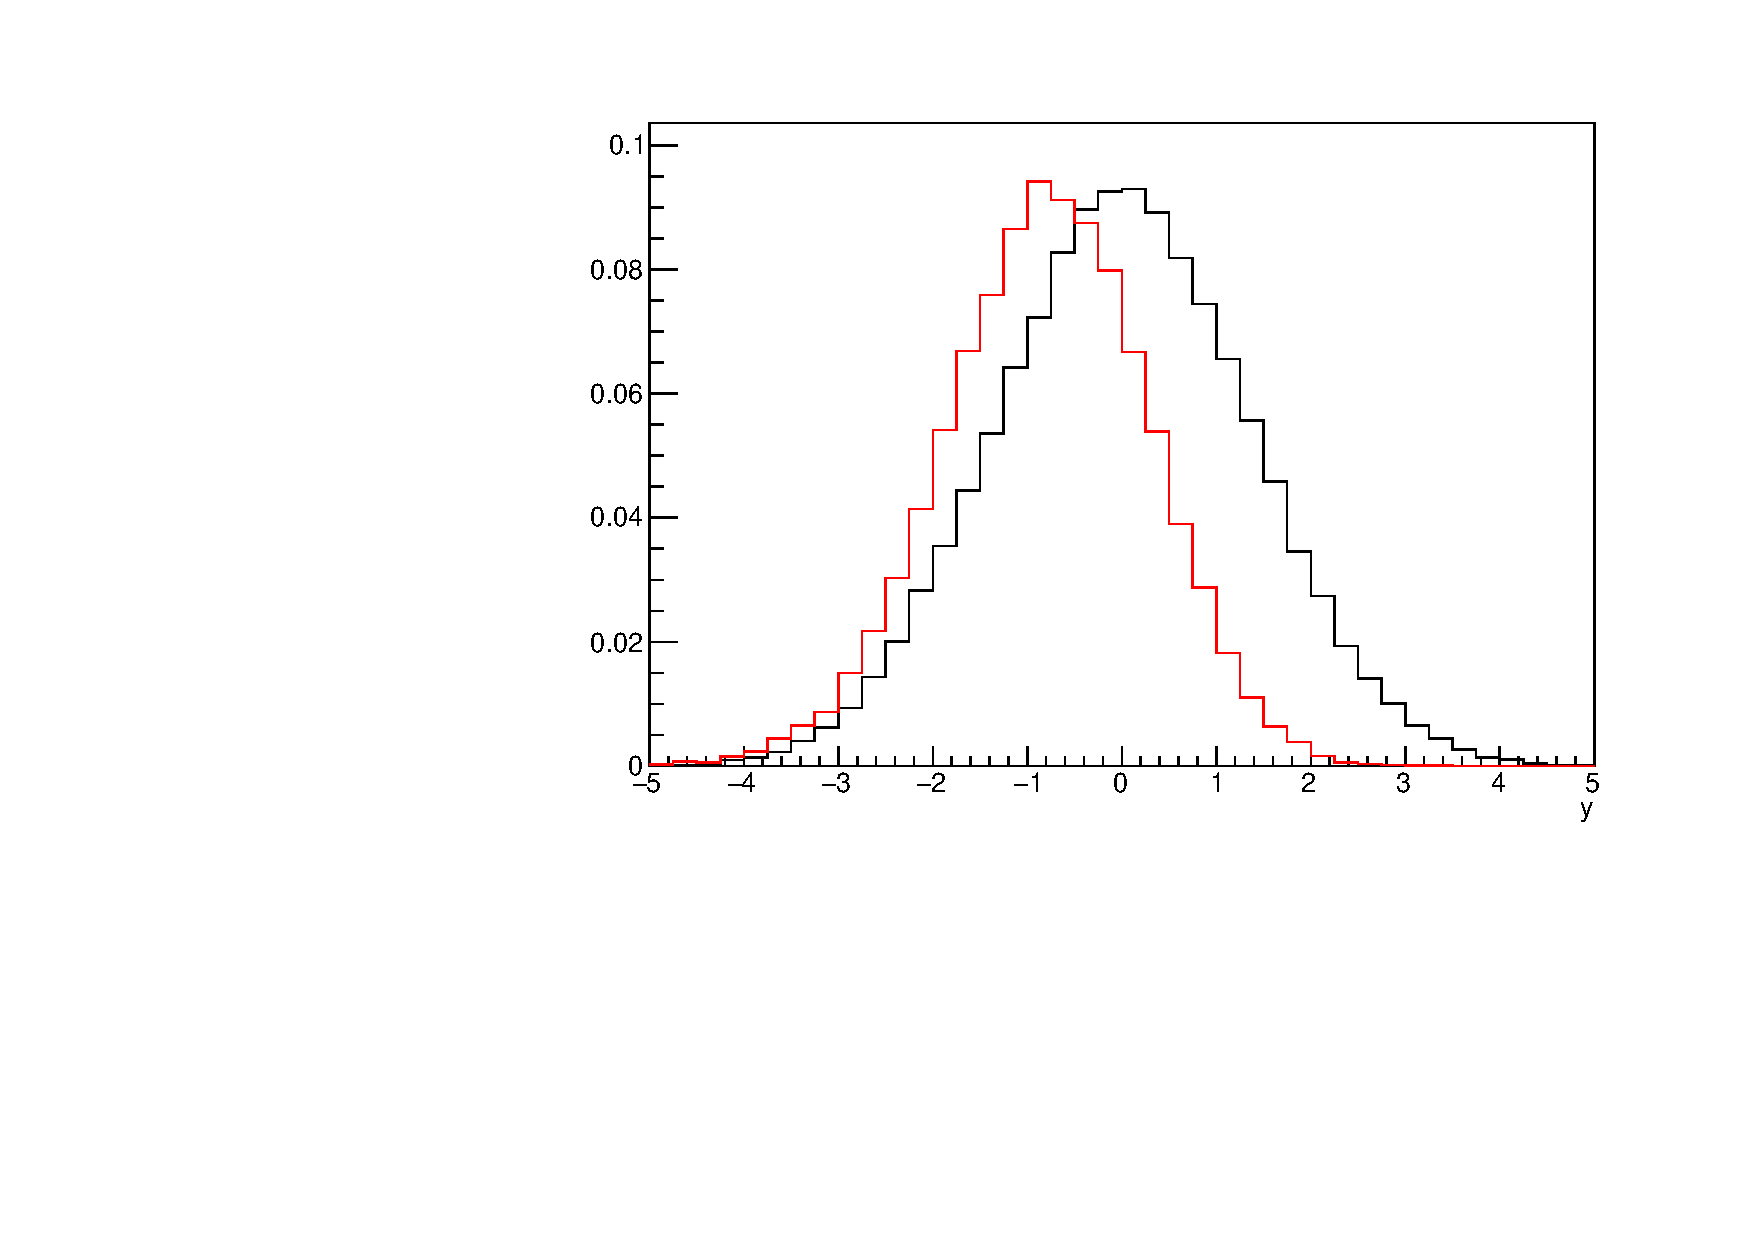
\includegraphics[width=\textwidth, trim={0mm 0mm 0mm 0mm}, clip,page=1]{Figures/MCMC/MCTechnique_Marginalisation1D_Double_Correlations.pdf}
  \end{subfigure}

  \caption{Left: The two-dimensional probability distribution for two correlated parameters \quickmath{x} and \quickmath{y}. The red distribution shows the two-dimensional probability distribution when \quickmath{0 \leq x \leq 5}. Right: The marginalised probability distribution for the \quickmath{y} parameter found when requiring the \quickmath{x} to be bound between \quickmath{-5 \leq x \leq 5} and \quickmath{0 \leq x \leq 5} for the black and red distribution, respectively.}
  \label{fig:MCMC_MCTechniqueMarginalisationProblems}
\end{figure}

\subsection{Parameter Estimation and Credible Intervals}
\label{sec:MarkovChainMonteCarlo_ParameterEstimation}

The purpose of this analysis is to determine the best fit values for the oscillation parameters that the beam and atmospheric samples are sensitive to: \quickmath{\sin^{2}(\theta_{23})}, \quickmath{\sin^{2}(\theta_{13})}, \quickmath{\Delta m^{2}_{32}}, and \quickmath{\delta_{CP}}.
%Typically, the results presented take the form of one or two-dimension marginalised probability distributions for the appearance (\quickmath{\sin^{2}(\theta_{13})} and \quickmath{\delta_{CP}}) and disappearance (\quickmath{\sin^{2}(\theta_{23})} and \quickmath{\Delta m^{2}_{32}}) parameters.
The posterior probability density, taken from the output MCMC chain, is binned in these parameters. The parameter best-fit point is then taken to be the value that has the highest posterior probability. This is performed in both one and two-dimensional projections.

However, the single best-fit point in a given parameter is not of much use on its own. We would also like to determine the uncertainty, or credible interval, on that best-fit point. The definition of the \quickmath{1\sigma} credible interval is that we have \quickmath{68\%} belief that the parameter is within those bounds. For a more generalised definition, the credible interval is the region, \quickmath{R}, of the posterior distribution that contains a specific fraction of the total probability, such that

\begin{equation}
\int_{R} P(\theta|D)d\theta = \alpha
\end{equation}

Where \quickmath{\theta} is the parameter on which we calculate the credible interval. This technique then calculates the \quickmath{\alpha \times 100\%} credible interval.

In practice, this analysis uses the highest posterior density (HPD) credible intervals which are calculated through the following method. First, the probability distribution is area-normalised such that it has an integrated area equal to \quickmath{1.0}. The bins of probability are then summed from the highest to lowest until the sum exceeds the \quickmath{1\sigma} level (\quickmath{0.68} in this example). This process is repeated for a range of credible intervals, notably the \quickmath{1\sigma}, \quickmath{2\sigma} and \quickmath{3\sigma} along with other levels where the critical values for each level can be found in \cite{Particle_Data_Group2020-ms}. This process can be repeated for the two-dimensional probability distributions by creating two-dimensional contours of credible intervals rather than a one-dimensional result. 

\subsection{Bayesian Model Comparisons}
\label{sec:MarkovChainMonteCarlo_BayesTheorem}
Due to the matter resonance, this analysis has some sensitivity to the mass hierarchy of neutrino states (whether \quickmath{\Delta m^{2}_{32}} is positive or negative) and the octant of \quickmath{\sin^{2}(\theta_{23})}. The Bayesian approach utilised within this analysis gives an intuitive method of model comparison by determining which hypothesis is most favourable. Taking the ratio of \autoref{eq:MarkovChainMonteCarlo_PosteriorDistributionReduced} for the two hypotheses of normal hierarchy, \quickmath{NH}, and inverted hierarchy, \quickmath{IH}, gives

\begin{equation}
  \frac{P(\vec{\theta}_{NH}|D)}{P(\vec{\theta}_{IH}|D)} = \frac{P(D|\vec{\theta}_{NH})}{P(D|\vec{\theta}_{IH})} \times \frac{P(\vec{\theta}_{NH})}{P(\vec{\theta}_{IH})}.
\end{equation}

The middle term defines the Bayes factor, \quickmath{B(\text{NH}/\text{IH})}, which is a data-driven interpretation of how strong the data prefers one hierarchy to the other. For this analysis, equal priors on both mass hierarchy hypotheses are chosen (\quickmath{P(\vec{\theta}_{NH}) = P(\vec{\theta}_{IH})} = 0.5). In practice, the MCMC chain proposes a value of \quickmath{|\Delta m^{2}_{32}|} and then applies a \quickmath{50\%} probability that the value is sign flipped. Consequently, the Bayes factor can be calculated from the ratio of the probability density in either hypothesis. This equates to counting the number of steps taken in the normal and inverted hierarchies and taking the ratio. The same approach can be taken to compare the upper octant (UO) compared to the lower octant (LO) hypothesis of \quickmath{\sin^{2}(\theta_{23})}.

\begin{table}[ht!]
    \centering
    \begin{tabular}{c|c|l}
      \hline
      $\log_{10}(B_{AB})$ & $B_{AB}$ & Strength of Preference \\
      \hline
      \hline
      \quickmath{<0.0} & \quickmath{<1} & No preference for hypothesis A (Supports hypothesis B) \\
      \quickmath{0.0 - 0.5} & \quickmath{1.0 - 3.16} & Preference for hypothesis A is weak \\
      \quickmath{0.5 - 1.0} & \quickmath{3.16 - 10.0} & Preference for hypothesis A is substantial \\
      \quickmath{1.0 - 1.5} & \quickmath{10.0 - 31.6} & Preference for hypothesis A is strong \\
      \quickmath{1.5 - 2.0} & \quickmath{31.6 - 100.0} & Preference for hypothesis A is very strong \\
      \quickmath{>2.0 }& \quickmath{>100.0} & Decisive preference for hypothesis A \\
      \hline
      \hline
      
      \hline
    \end{tabular}
    \caption{Jeffreys scale for strength of preference for two models \quickmath{A} and \quickmath{B} as a function of the calculated Bayes factor (\quickmath{B_{AB} = B(A/B)}) between the two models \cite{Jeffreys:1939xee}. The original scale is given in terms of \quickmath{\log_{10}(B(A/B))} but converted to linear scale for easy comparison throughout this thesis.}
    \label{tab:MarkovChainMonteCarlo_JeffreysScale}
\end{table}

Whilst the value of the Bayes factor should always be shown, the Jeffreys scale \cite{Jeffreys:1939xee} (highlighted in \autoref{tab:MarkovChainMonteCarlo_JeffreysScale}) gives an indication of the strength of preference for one model compared to the other. Other interpretations of the strength of preference of a model exist, e.g. the Kass and Raferty Scale \cite{Kass1995-nl}.

\subsection{Comparison of MCMC Output to Expectation}
\label{sec:MarkovChainMonteCarlo_Predictives}

To ensure the fit is performing well, a best-fit spectrum is produced using the posterior probability distribution and compared with the data, allowing easy by-eye comparisons to be made. A simple method of doing this is to perform a comparison in the fitting parameters (For instance, the reconstructed neutrino energy and lepton direction for T2K far detector beam samples) of the spectra generated by the MCMC chain to `data'. This `data' could be true data or some variation of Monte Carlo prediction. This allows easy comparison of the MCMC probability distribution to the data. To perform this, \quickmath{N} steps from the post-burnin MCMC chain are randomly selected. From these, the Monte Carlo prediction at each step is generated by reweighting the model parameters to the values specified at that step. Due to the probability density being directly correlated with the density of steps in a certain region, parameter values close to the best fit value are most likely to be selected.

In practice, for each bin of the fitting parameters has a probability distribution of event rates, with one entry per sampled MCMC step. This distribution is binned where the bin with the highest probability is selected as the mean and an error on the width of this probability distribution is calculated using the approach highlighted in \autoref{sec:MarkovChainMonteCarlo_ParameterEstimation}. Consequently, the best fit distribution in the fit parameter is not necessarily that which would be attained by reweighting the Monte Carlo prediction to the most probable parameter values.

A similar study can be performed to illustrate the freedom of the model parameter space prior to the fit. This can be done by throwing parameter values from the prior uncertainty of each parameter.
%This becomes troublesome for parameters with no prior uncertainty as the range is technically infinite. Where applicable solutions to remove these have been addressed.

\chapter{Simulation, Reconstruction, and Event Reduction}
\label{chap:Simulations}

As a crucial part of the oscillation analysis, an accurate prediction of the expected neutrino spectrum at the far detector is required. This includes modeling the flux generation, neutrino interactions, and detector effects. All of the simulation packages required to do this are briefly described in \autoref{sec:Simulations_Simulation}. The reconstruction of neutrino events in the far detector, including the \texttt{fiTQun} algorithm, is documented in \autoref{sec:Simulation_Reconstruction}. This also includes data quality checks of the SK-V data which the author performed for the T2K oscillation analysis presented at the Neutrino 2020 conference \cite{Dunne2020-uf}. Finally, \autoref{sec:Simulations_Reduction} describes the steps taken in the SK detector to trigger on events of interest whilst removing the comparatively large rate of cosmic ray muon events.

\section{Simulation}
\label{sec:Simulations_Simulation}

In order to generate a Monte Carlo prediction of the expected event rate at the far detector, all the processes in the beam and atmospheric fluxes, neutrino interaction, and detector need to be modeled. %Each of these parts is individually modeled and each of them is detailed below.

\subsection{Neutrino Flux}

The beamline simulation consists of three distinct parts: the initial hadron interaction modeled by FLUKA \cite{fluka2011}, the target station geometry and particle tracking performed by JNUBEAM, \cite{geant3, PhysRevD.87.012001} and any hadronic re-interactions simulated by GCALOR \cite{gcalor}. The primary hadronic interactions are \quickmath{O(10)\text{GeV}}, where FLUKA matches external cross-section data better than GCALOR \cite{t2k_tn_flux}. However, FLUKA is not very adaptable so a small simulation is built to model the interactions in the target and the output is then passed to JNUBEAM and GCALOR for propagation. The hadronic interactions are tuned to data from the NA61/SHINE \cite{Abgrall_2011, Abgrall_2012, NA61_pions_rep} and HARP \cite{harp} experiments. The tuning is done by reweighting the FLUKA and GCALOR predictions to match the external data and cross-section measurements, based on final state particle kinematics \cite{t2k_tn_flux}. The culmination of this simulation package generates the predicted flux for neutrino and antineutrino beam modes which are illustrated in \autoref{fig:T2KSKExp_T2K_NuFluxPerMode}.

The atmospheric neutrino flux is simulated by the HKKM model \cite{Honda_2007, Honda:2011}. The primary cosmic ray flux is tuned to AMS \cite{Blau2002} and BESS \cite{Haino2004} data assuming the US-standard atmosphere `76 \cite{USStandardAtm} density profile and includes geomagnetic field effects. The primary cosmic rays interact to generate pions and muons. The interaction of these secondary particles to generate neutrinos is handled by DPMJET-III \cite{Roesler2001} for energies above \quickmath{32\text{GeV}} and JAM \cite{Niita2006, Honda:2011} for energies below that value \cite{Gaisser2002-gl}. These hadronic interactions are tuned to BESS and L3 data \cite{Sanuki_2002, Achard_2004} using the same methodology as the tuning of the beamline simulation. The energy and cosine zenith predictions of \quickmath{\nu_{e}, \bar{\nu}_{e}, \nu_{\mu}, \bar{\nu}_{\mu}} flux are given in \autoref{fig:NeutrinoOscillationPhysics_AtmosphericNeutrinoFlux} and \autoref{fig:NeutrinoOscillationPhysics_NuFluxZenithAngleDep}, respectively. The flux is approximately symmetrical and peaked around the horizon (\quickmath{\cos(\theta_{Z}) = 0.0}). This is because horizontally-going pions and kaons can travel further than their vertically-going counterparts resulting in a larger probability of decaying to neutrinos. The symmetry is broken in lower-energy neutrinos due to geomagnetic effects, which modify the track of the primary cosmic rays. Updates to the HKKM model are currently ongoing \cite{Sato2022-ss}.

\subsection{Neutrino Interaction}

Once a flux prediction has been made for all three detectors, NEUT 5.4.0 \cite{Hayato2021, neut} models the interactions of the neutrinos in the detectors. For the purposes of this analysis, quasi-elastic (QE), meson exchange (MEC), single meson production (PROD, RES), coherent pion production (COH), and deep inelastic scattering (DIS) interactions are simulated. These interaction categories can be further broken down by whether they were propagated via a \quickmath{W^{\pm}} boson in Charged Current (CC) interactions or via a \quickmath{Z^{0}} boson in Neutral Current (NC) interactions. CC interactions have a charged lepton in the final state, which can be flavour-tagged in reconstruction to determine the flavour of the neutrino. In contrast, NC interactions have a neutrino in the final state so no flavour information can be determined from the observables left in the detector after an interaction. This is the reason why neutrinos that interact through NC modes are assumed to not oscillate within this analysis. Both CC and NC interactions are modeled for all the above interaction categories, other than MEC interactions which are only modeled for CC events. 
%As the SK detector is only sensitive to charged particles above Cherenkov threshold, all charged current interactions are simulated whilst only neutral current processes that can produce charged particles (NCDIS, NCCOH, and NCPROD including $\pi^{0}$ production) are modeled. NC MEC interactions can only produce charged particles through secondary re-interactions which is a low cross-section process.

\begin{figure}[h]
  \begin{subfigure}[t]{0.8\textwidth}
    \includegraphics[width=\textwidth, trim={0mm 0mm 0mm 0mm}, clip,page=1]{Figures/Simulations/NEUTCrossSection.pdf}
  \end{subfigure}
  \caption{The NEUT prediction of the \quickmath{\nu_{\mu}}-H2O cross-section overlaid on the T2K \quickmath{\nu_{\mu}} flux. The charged current (black, solid) and neutral current (black, dashed) inclusive, charged current quasi-elastic (blue, solid), charged current 2p2h (blue, dashed), charged current single pion production (pink), and charged current multi--\quickmath{\pi} and DIS (Purple) cross-sections are illustrated. Figure taken from \cite{Hayato2021}.}
  \label{fig:Simulations_CrossSection}
\end{figure}

As illustrated in \autoref{fig:Simulations_CrossSection}, CCQE interactions dominate the cross-section of neutrino interactions around \quickmath{E_{\nu} \sim 0.5 \text{GeV}}. The NEUT implementation adopts the Llewellyn Smith \cite{llewelyn-smith} model for neutrino-nucleus interactions, where the nuclear ground state of any bound nucleons (neutrino-oxygen interactions) is approximated by a spectral-function \cite{Benhar1989} model that simulates the effects of Fermi momentum and Pauli blocking. The cross-section of QE interactions is controlled by vector and axial-vector form factors parameterised by the BBBA05 \cite{bbba05} model and a dipole form factor with \quickmath{M_{A}^{QE} = 1.21\text{GeV}} fit to external data \cite{Aguilar_Arevalo_2010}, respectively. NEUT implements the Valencia \cite{nieves2} model to simulate MEC events, where two nucleons and two holes in the nuclear target are produced (often called 2p2h interactions). A nuclear hole is defined as an unoccupied single-particle state below the Fermi level \cite{Gillet1964}.

For neutrinos of energy \quickmath{O(1)\text{GeV}}, PROD interactions become dominant. These predominantly produce charged and neutral pions although \quickmath{\gamma}, kaon, and \quickmath{\eta} production is also considered. To simulate these interactions, the Berger-Sehgal \cite{PhysRevD.76.113004} model is implemented within NEUT. It simulates the excitation of a nucleon from a neutrino interaction, production of an intermediate baryon, and the subsequent decay to a single meson or \quickmath{\gamma}. Pions can also be produced through COH interactions, which occur when the incoming neutrino interacts with the entire oxygen nucleus leaving a single pion outside of the nucleus. NEUT utilises the Berger-Sehgal \cite{Berger_Sehgal_coh} model to simulate these COH interactions.

DIS and multi-\quickmath{\pi} producing interactions become the most dominant for energies \quickmath{>O(5)\text{GeV}}. PYTHIA \cite{Sjstrand1994} is used to simulate any interaction with invariant mass \quickmath{W > 2\text{GeV/c}^{2}}, which produces at least one meson. For any interaction which produces at least two mesons but has \quickmath{W < 2\text{GeV/c}^{2}}, the Bronner model is used \cite{Bronner2016}. Both of these models use Parton distribution functions based on the Bodek-Yang model \cite{Gl_ck_1998,10.48550/arxiv.1011.6592,10.48550/arxiv.1012.0261}. 

\begin{figure}[h]
  \begin{subfigure}[t]{0.8\textwidth}
    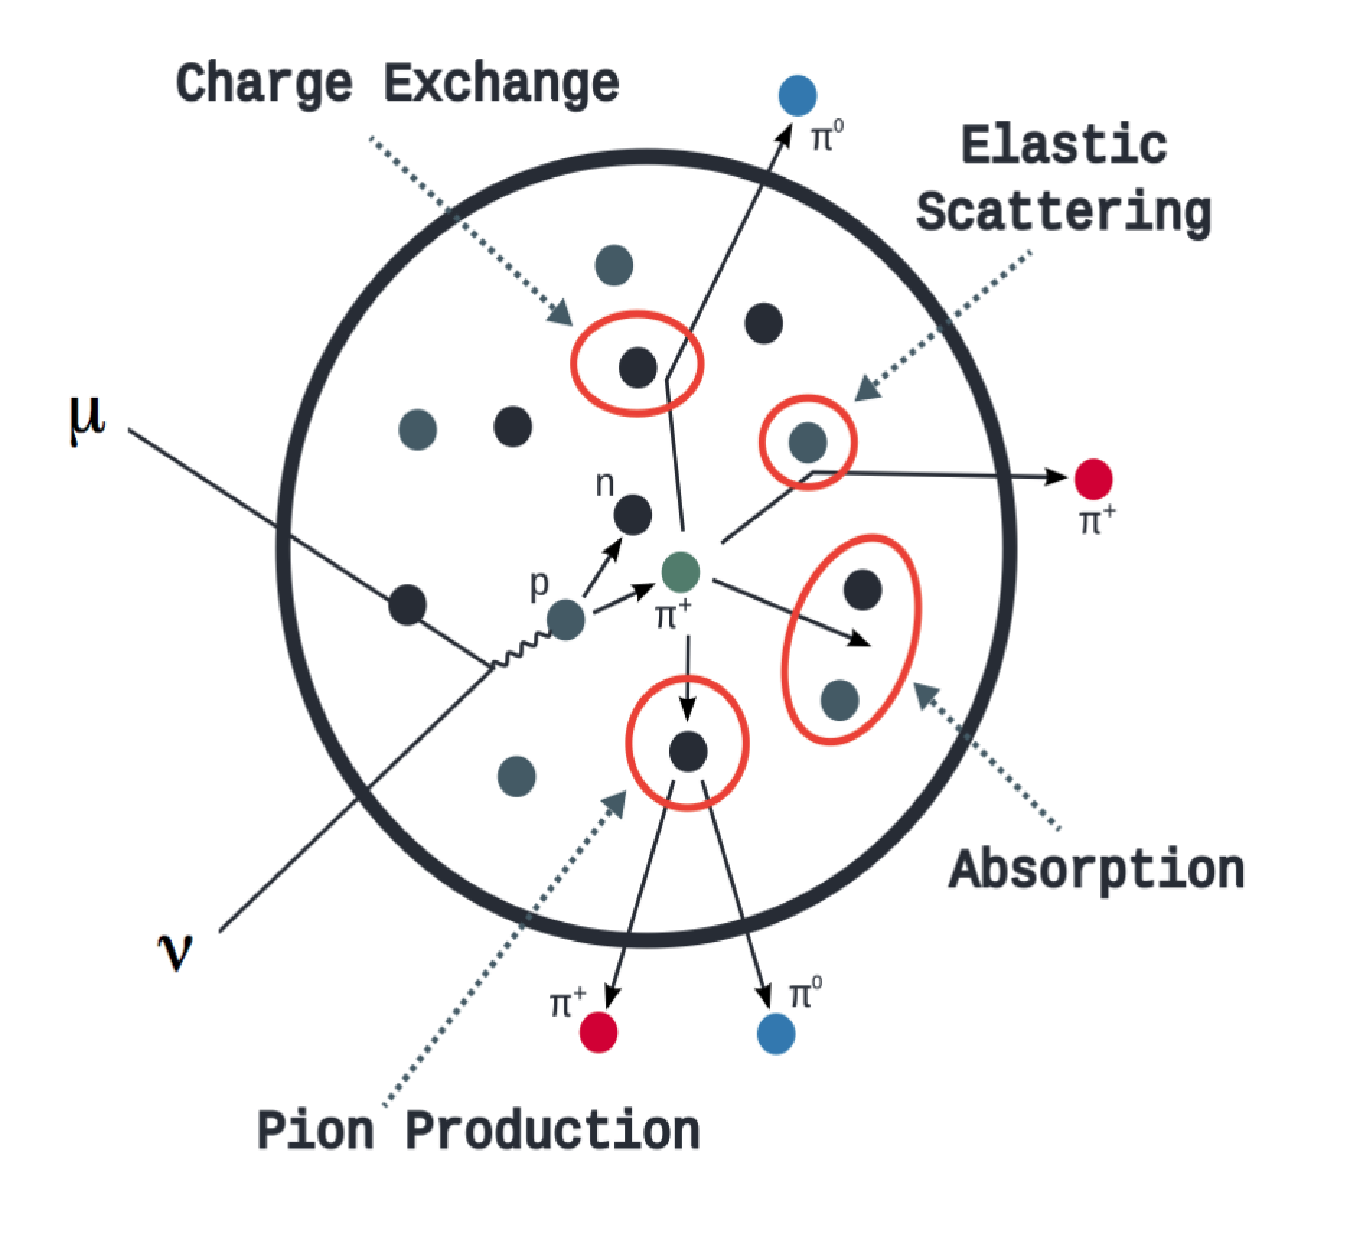
\includegraphics[width=\textwidth, trim={0mm 0mm 0mm 0mm}, clip,page=1]{Figures/Simulations/FSIDiagram.pdf}
  \end{subfigure}
  \caption{Illustration of the various processes which a pion can undergo before exiting the nucleus. Taken from \cite{10.48550/arxiv.1602.05299}.}
  \label{fig:Simulations_FSIDiagram}
\end{figure}

Any pion that is produced within the nucleus can re-interact through final state interactions before it exits, as illustrated by the scattering, absorption, production, and exchange interactions in \autoref{fig:Simulations_FSIDiagram}. These re-interactions alter the observable particles within the detector. For instance, if the charged pion from a CC PROD interaction is absorbed, the observables would mimic a CC QE interaction. To simulate these effects, NEUT uses a semi-classical intranuclear cascade model \cite{Hayato2021}. This cascade functions by stepping the pion through the nucleus in fixed-length steps equivalent to \quickmath{dx = R_{N}/100}, where \quickmath{R_{N}} is the radius of the nucleus. At each step, the simulation allows the pion to interact through scattering, charged exchange, absorption, or production with an interaction-dependent probability calculated from a fit to external data \cite{PhysRevD.99.052007}. This cascade continues until the pion is absorbed or exits the nucleus.

\subsection{Detector}

Once the final state particle kinematics have been determined by NEUT, they are passed into the detector simulation. The near detectors, ND280 and INGRID, are simulated using a \texttt{GEANT4} package \cite{t2k_det,geant4} to simulate the detector geometry, particle tracking, and energy deposition. The response of the detectors is simulated using the elecSim package \cite{t2k_det}.

The far detector simulation, based upon the original Kamiokande experiment software, uses the \texttt{GEANT3}-based SKDETSIM \cite{Brun:1987ma,t2k_det} package. This simulates the interactions of particles in the water as well as Cherenkov light production. The water quality and PMT calibration measurements detailed in \autoref{subsec:T2KSKExp_SKCalibration} are also used within this simulation to make accurate predictions of the detector response.

Any event which generates optical photons that occurs in SK will be observed by the PMT array, where each PMT records the time and accumulated charge. This recorded information is shown in event displays similar to those illustrated in \autoref{fig:Simulations_SKEventDisplays} for simulated Monte Carlo events. To be useful for physics analyses, this series of PMT hit information needs to be reconstructed to determine the number and identity of particles and their kinematics (or track parameters): four-vertex, direction, and momentum. The reconstruction uses the fact that the charge and timing distribution of photons generated by a particular particle in an event is dependent upon its initial kinematics. Electron and muon rings are distinguished by their ``fuzziness''. Muons are heavier and less affected by scattering or showering meaning they typically produce ``crisp'' rings. Electrons are more likely to interact via electromagnetic showering or scattering which results in larger variations of their direction from the initial direction. Consequently, electrons typically produce ``fuzzier'' rings compared to muons. 

\begin{figure}[h]
  \begin{subfigure}[t]{0.5\textwidth}
    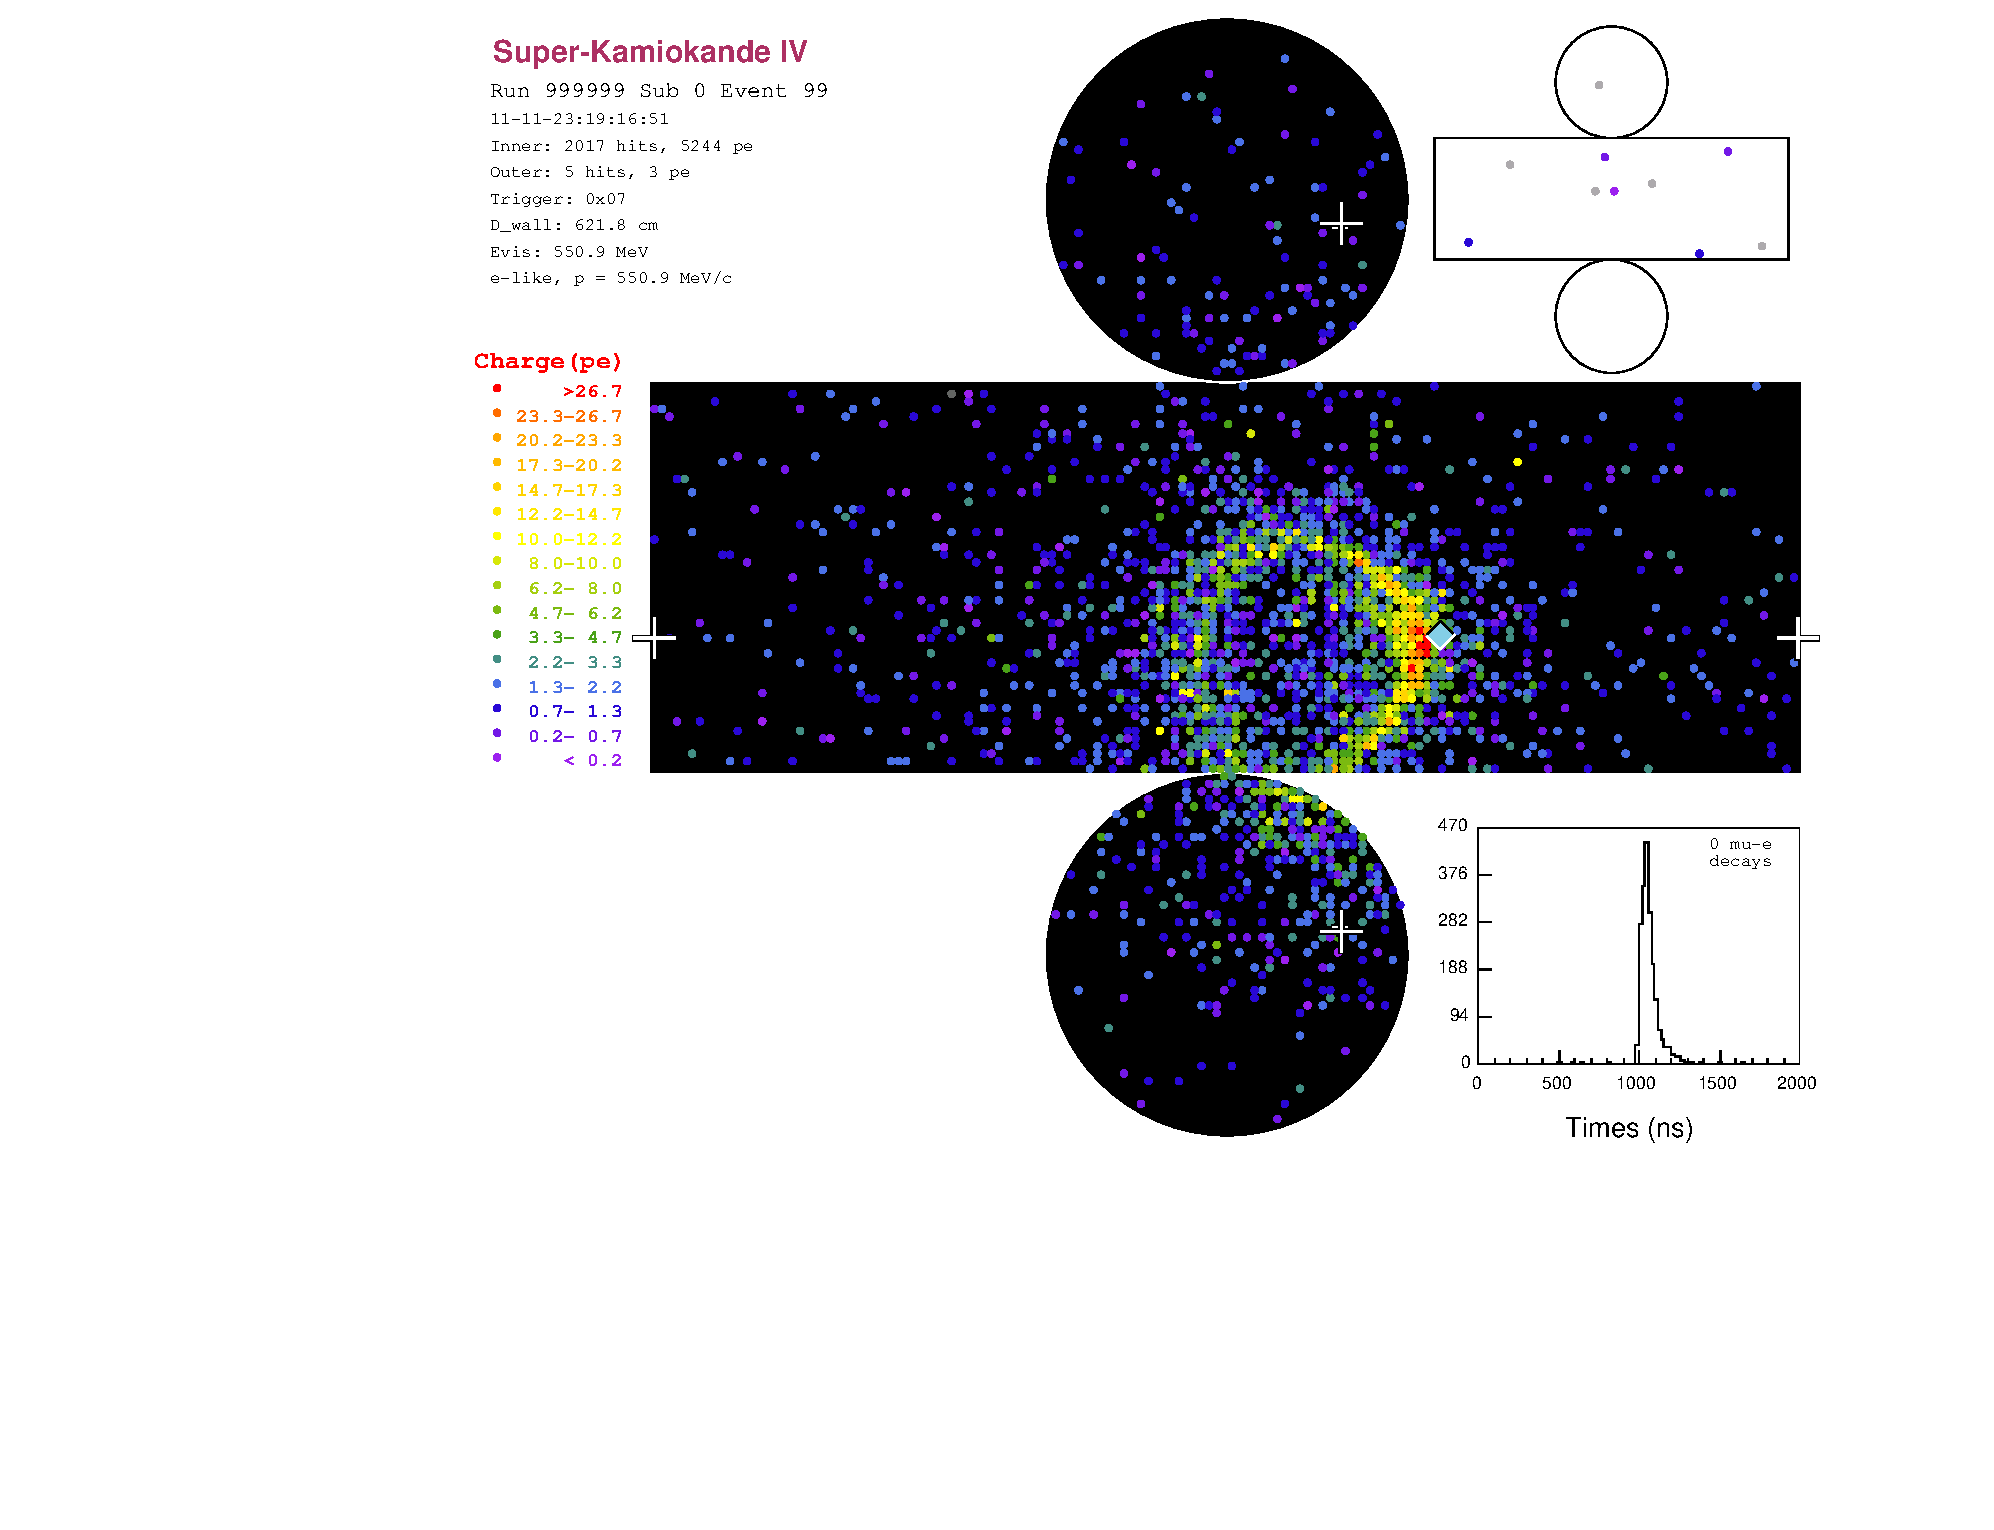
\includegraphics[width=\textwidth, trim={0mm 0mm 0mm 0mm}, clip,page=1]{Figures/Simulations/NuECandidate.pdf}
    \subcaption{\quickmath{\nu_{e}}}
  \end{subfigure}%
  \begin{subfigure}[t]{0.5\textwidth}
    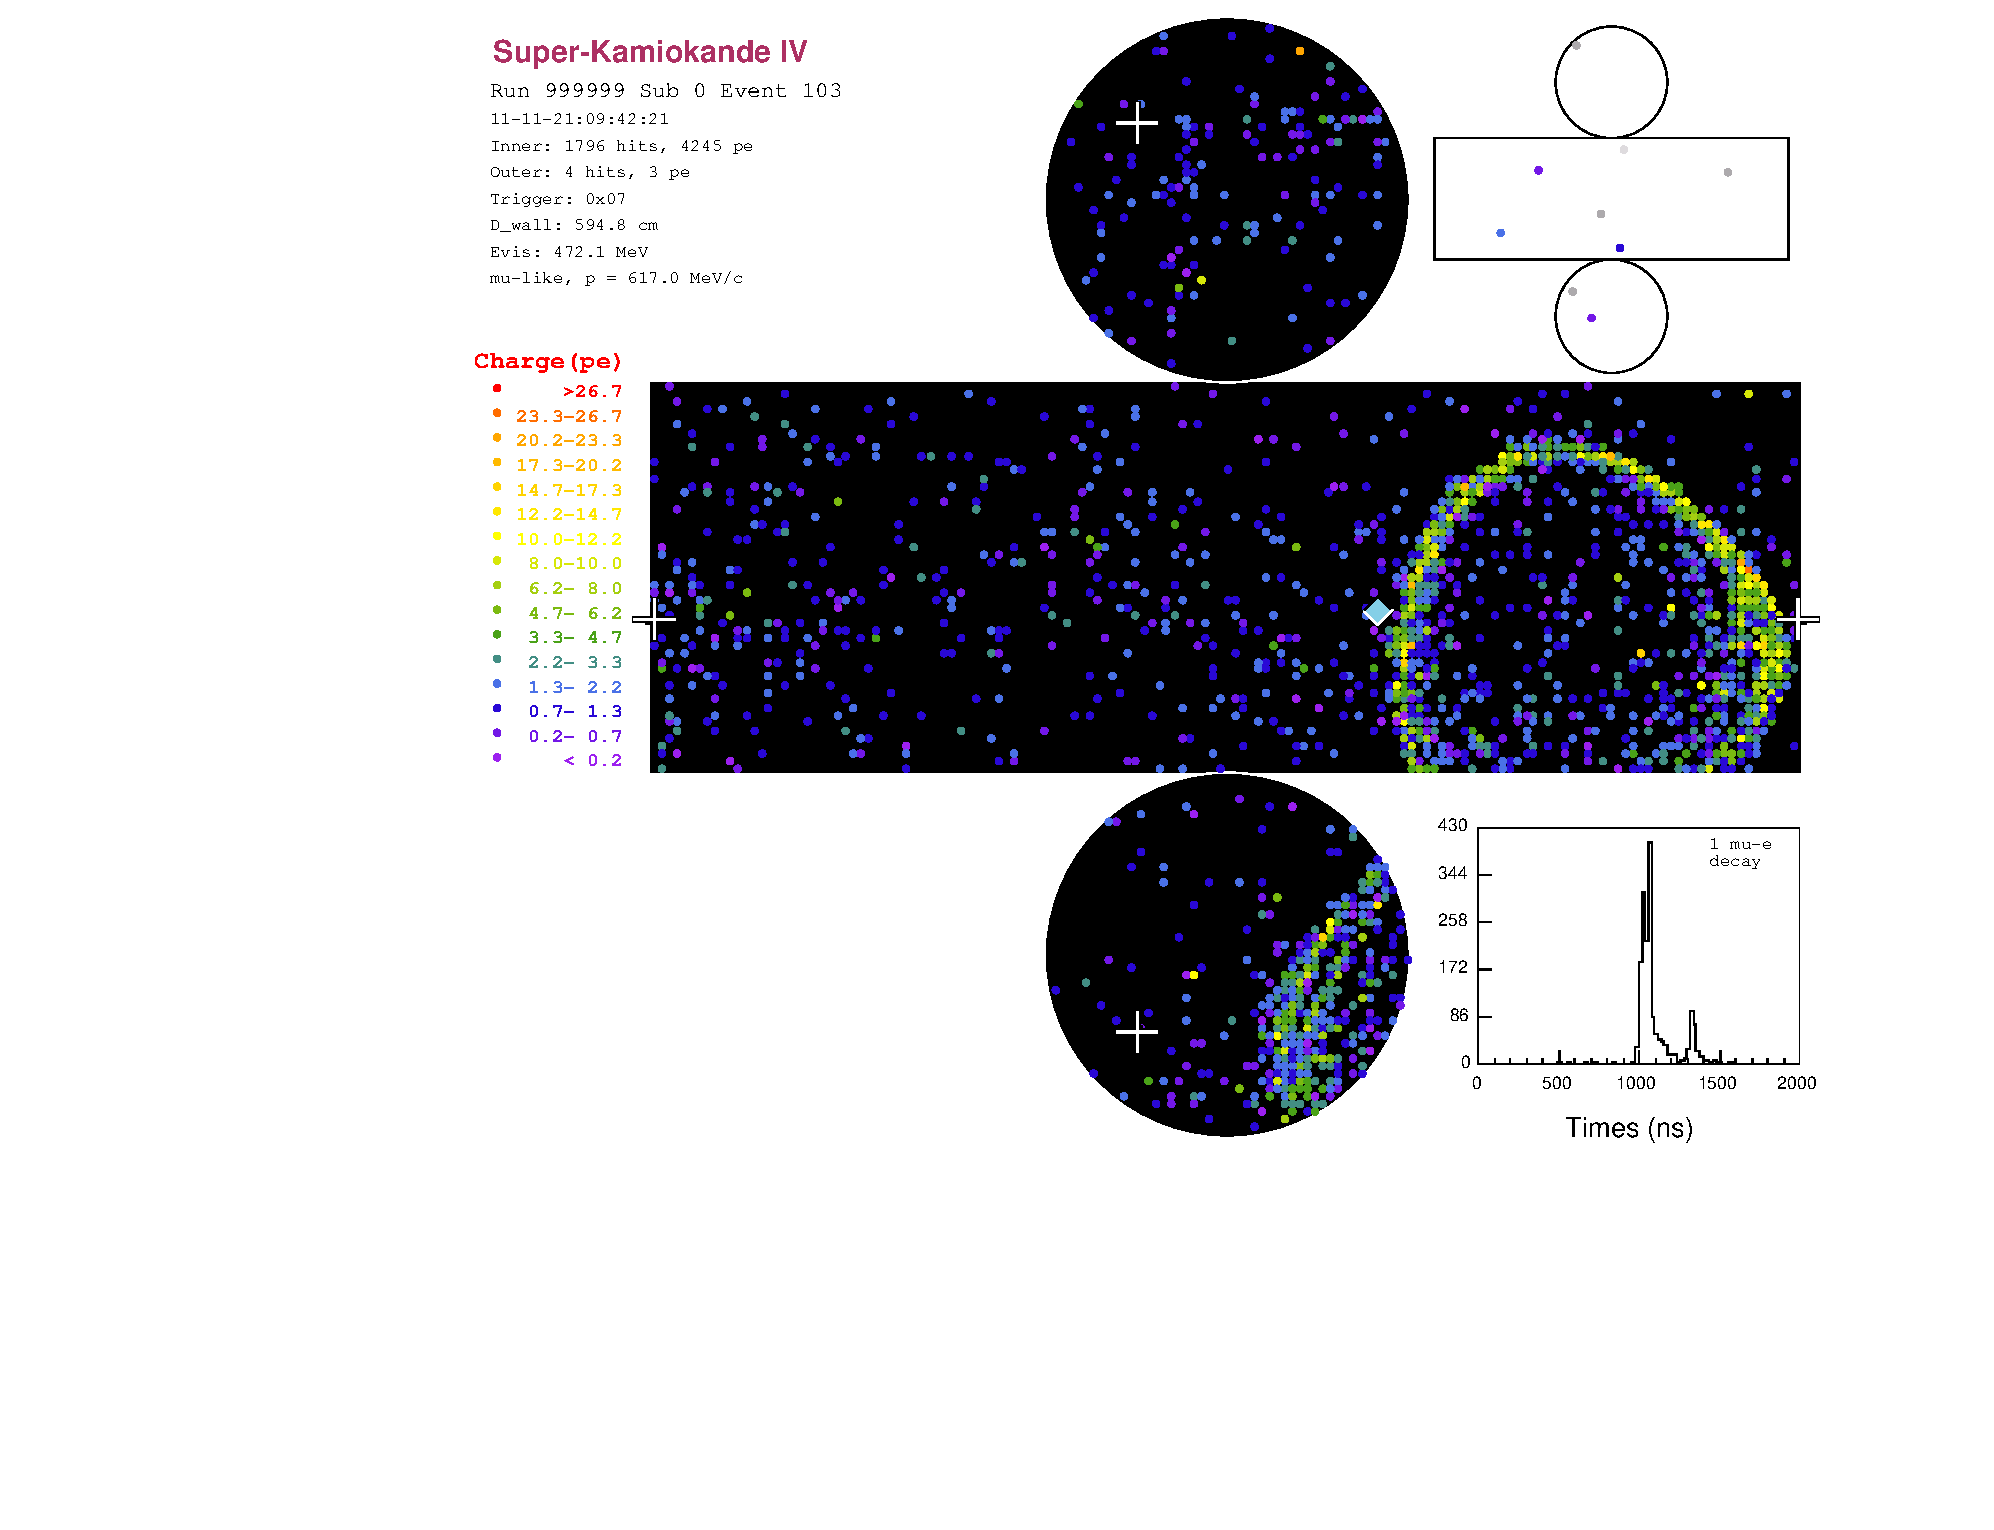
\includegraphics[width=\textwidth, trim={0mm 0mm 0mm 0mm}, clip,page=1]{Figures/Simulations/NuMuCandidate.pdf}
    \subcaption{\quickmath{\nu_{\mu}}}
  \end{subfigure}
  \caption{Event displays from Monte Carlo simulation at Super Kamiokande illustrating the ``crisp'' ring from a muon and the typically ``fuzzier'' electron ring. Each pixel represents a PMT and the color scheme denotes the accumulated charge deposited on that PMT. Figures taken from \cite{t2k_tn_219}.}
  \label{fig:Simulations_SKEventDisplays}
\end{figure}

\newpage
\section{Event Reconstruction at SK}
\label{sec:Simulation_Reconstruction}

%For the purposes of this analysis, the \texttt{fiTQun} reconstruction algorithm is utilised. Its core function is to compare a prediction of the accumulated charge and timing distribution from each PMT, generated for a particular particle identity and track parameters, to that observed in the neutrino event. It determines the preferred values by minimising a likelihood function which includes information from PMTs which were hit and those that were not hit. The \texttt{fiTQun} algorithm improves upon the \texttt{APFit} reconstruction algorithm which has been used for many previous SK analyses. \texttt{APFit} fits the vertex from timing information and then fits the momentum and direction of the particle from PMT hits within a \quickmath{43\deg} Cherenkov cone (which assumes an ultra-relativistic particle). It then fits the particle identity once the track parameters have been fit. Conversely, \texttt{fiTQun} performs a simultaneous fit of particle kinematics and identity, improving both the accuracy of the fit parameters and the rejection of neutral current \quickmath{\pi^{0}} events \cite{Abe2018, Abe2015}. The \texttt{fiTQun} algorithm is based on the key concepts of the MiniBooNE reconstruction algorithm \cite{Patterson_2009} and is described in \cite{t2k_tn_146} which is summarised below.

%An event in SK can consist of multiple ``sub-events''. For example, a muon neutrino interaction will generate a muon which will subsequently decay into an electron. Both the muon and electron can generate Cherenkov photons but both subevents need to be reconstructed separately. Therefore, to avoid assigning photons generated by the decay-electron to the muon, each event is divided into time clusters, termed ``subevents'', where subevent is defined to contain at most one hit for each PMT. To find the subevents, a vertex goodness metric is calculated for some vertex position \quickmath{\vec{x}} and time \quickmath{t},

For the purposes of this analysis, the \texttt{fiTQun} reconstruction algorithm \cite{t2k_tn_146} is utilised. Its core function is to compare a prediction of the accumulated charged and timing distribution from each PMT, generated for a particular particle identity, vertex, and momentum, to that observed in the neutrino event. It determines the preferred values by maximising a likelihood function (or minimising a negative log-likelihood function) which includes information from PMTs which were hit and those that were not hit. The \texttt{fiTQun} algorithm is based on the key concepts of the MiniBooNE reconstruction algorithm \cite{Patterson_2009}.

The \texttt{fiTQun} algorithm improves upon the previous \texttt{APFit} algorithm \cite{Shiozawa1999} which has been used for many previous SK analyses. \texttt{APFit} fits the vertex from timing information and then fits the direction of the particle from PMT hits within a \quickmath{43\deg} Cherenkov cone (assuming an ultra-relativistic particle) using a fitting estimator. A Hough transformation is used to find the radius of a ring (related to the momentum through \autoref{eq:T2KSKExp_CherenkovConeAngle}) as well as the number of rings contained within the event. The analysis presented here uses the \texttt{fiTQun} algorithm as it improves both the accuracy of the fit parameters and the rejection of neutral current \quickmath{\pi^{0}} events as compared to \texttt{APFit} \cite{Abe2018, Abe2015}.

Any event in SK can consist of prompt (or primary) and decay (or secondary) particles. For example, a charged current muon neutrino interaction can generate two particles that have the potential of generating Cherenkov photons (assuming the proton is below the Cherenkov threshold): the prompt muon, and the michel-electron which is produced on average \quickmath{2.2\mu\text{s}} later. To correctly reconstruct all particles within an event, it is divided into time clusters which are called ``subevents''. Subevents after the primary subevent are considered to be decay electrons.

The main steps of the \texttt{fiTQun} reconstruction algorithm are:

\begin{itemize}
\item \textbf{Vertex pre-fitting}: An estimate of the vertex is made using a goodness-of-fit metric based on PMT hit times
\item \textbf{Peak finding}: The initial time of each subevent is determined by clustering events by time residuals
\item \textbf{Single-ring fits}: Given the pre-fit vertex and estimated time of interaction, a maximum likelihood technique searches for a single particle generating light. Electron, muon, charged pion, and proton hypotheses are considered
\item \textbf{Multi-ring fits}: Seeded from the single-ring fits, hypotheses with multiple light-producing particles are considered using the same maximum likelihood technique. Electron-like or charged pion-like rings are added until the likelihood stops improving
\end{itemize}

To find all the subevents in an event, a vertex goodness metric is calculated for some vertex position \quickmath{\vec{x}} and time \quickmath{t},

%The number of subevents is equal to the number of decay electrons plus one (the primary event).

\begin{equation}
  G(\vec{x},t) = \sum^{\text{hit PMTs}}_{i} \exp \left( - \frac{1}{2} \left( \frac{T_{Res}^{i}(\vec{x},t)}{\sigma} \right)^{2} \right),
\end{equation}

where

\begin{equation}
  T_{Res}^{i}(\vec{x},t) = t^{i} - t - \left| R^{i}_{PMT} - \vec{x} \right|/c_{n},
\end{equation}

is the residual hit time. It is the difference in time between the PMT hit time \quickmath{t^{i}}, of the \quickmath{i^{th}} PMT, and the expected time of the PMT hit if the photon was emitted at the vertex. \quickmath{R^{i}_{PMT}} is the position of the \quickmath{i^{th}} PMT, \quickmath{c_{n}} is the speed of light in water and \quickmath{\sigma = 4\text{ns}} which is comparable to the time resolution of the PMT. When the proposed fit values of time and vertex are close to the true values, \quickmath{T_{Res}^{i}(\vec{x},t)} tends to zero resulting in subevents appearing as spikes in the goodness metric. The proposed fit vertex and time are grid-scanned, and the values which maximise the goodness metric are selected as the ``pre-fit vertex''. Whilst this predicts a vertex for use in the clustering algorithm, the final vertex is fit using the higher-precision maximum likelihood method described below.

Once the pre-fit vertex has been determined, the goodness metric is scanned as a function of \quickmath{t} to determine the number of subevents. A peak-finding algorithm is then used on the goodness metric. This requires the goodness metric to exceed some threshold and drop below a reduced threshold before any subsequent additional peaks are considered. The thresholds are set such that the rate of false peak finding is minimised while still attaining good data to Monte Carlo agreement. To improve performance, the pre-fit vertex for each delayed subevent is re-calculated after PMT hits from the previous subevent are masked. This improves the decay-electron tagging performance. Once all subevents have been determined, the time window around each subevent is then defined by the earliest and latest time which satisfies \quickmath{-180 < T_{Res}^{i} < 800 \text{ns}}. The subevents and associated time windows are then used as seeds for further reconstruction.

For a given subevent, the \texttt{fiTQun} algorithm constructs a likelihood based on the accumulated charge \quickmath{q_{i}} and time information \quickmath{t_{i}} from the \quickmath{i^{th}} PMT,

\begin{equation}
  L(\Gamma, \vec{\theta}) = \prod^{\text{unhit}}_{j} P_{j}(\text{unhit}|\Gamma,\vec{\theta}) \prod^{\text{hit}}_{i} \{ 1 - P_{i}(\text{unhit}|\Gamma,\vec{\theta}) \}   f_{q}(q_{i} | \Gamma, \vec{\theta}) f_{t}(t_{i} | \Gamma, \vec{\theta}).
\end{equation}

Where \quickmath{\vec{\theta}} defines the track parameters: vertex position, direction vector and momenta, and \quickmath{\Gamma} represents the particle hypothesis. \quickmath{P_{i}(\text{unhit}|\Gamma,\vec{\theta})} is the probability of the \quickmath{i^{th}} tube to not register a hit given the track parameters and particle hypothesis. The charge likelihood, \quickmath{f_{q}(q_{i} | \Gamma, \vec{\theta})}, and time likelihood, \quickmath{f_{t}(t_{i} | \Gamma,\vec{\theta})}, represents the probability density function of observing charge \quickmath{q_{i}} and time \quickmath{t_{i}} on the \quickmath{i^{th}} PMT given the specified track parameters and particle hypothesis.

%As the generation and propagation of the optical photons are independent of the PMT and electronics response, it is natural to split the calculation into two. This split was also performed to . Firstly, the expected number of photoelectrons (or predicted charge), \quickmath{\mu_{i} = \mu_{i}(\vec{\theta},\Gamma)}, at the \quickmath{i^{th}} PMT is calculated. This value is then substituted into the likelihood function. This allows the charge likelihood density \quickmath{f_{q}(q_{i} | \mu_{i})} and unhit probability \quickmath{P_{i}(\text{unhit}|\mu_{i})} to be expressed via quantities that are only dependent on the response of the PMT. 

The predicted charge is calculated based on contributions from both the direct light and the scattered light. The direct light contribution is determined based on the integration of the Cherenkov photon profile along the track. PMT angular acceptance, water quality, and calibration measurements discussed in \autoref{subsec:T2KSKExp_SKCalibration} are included to accurately predict the charge probability density at each PMT. The scattered and reflected light is calculated in a similar way, although it includes a scattering function that depends on the vertex of the particle and the position of the PMT. The charge likelihood is calculated by comparing the prediction to the observed charge in the PMT, where the prediction is tuned to the PMT simulation.

The time likelihood is approximated to depend on the vertex \quickmath{\vec{x}}, direction \quickmath{\vec{d}}, and time \quickmath{t} of the track as well as the particle hypothesis. The expected time for PMT hits is calculated by assuming unscattered photons being emitted from the midpoint of the track, \quickmath{S_{mid}},

\begin{equation}
  t_{exp}^{i} = t + S_{mid}/c + |R_{PMT}^{i} - \vec{x} - S_{mid}\vec{d}|/c_{n},
\end{equation}

where \quickmath{c} is the speed of light in a vacuum. The time likelihood is then expressed in terms of the residual difference between the PMT hit time and the expected hit time, \quickmath{t_{Res}^{i} = t^{i} - t_{exp}^{i}}.
%As the first photon hit defines the PMT hit time, the time likelihood density profile is narrower for higher momenta particles which introduces a dependence on the predicted charge.
The particle hypothesis and momentum also affect the Cherenkov photon distribution. These parameters modify the shape of the time likelihood density since in reality not all photons are emitted at the midpoint of the track. As with the charge likelihood, the contributions from both the direct and scattered light to the time likelihood density are calculated separately, which are both calculated from particle gun Monte Carlo studies.

The track parameters and particle identity which maximise \quickmath{L(\Gamma , \vec{\theta})} are defined as the best-fit parameters. In practice MINUIT \cite{James:2296388} is used to minimise the value of \quickmath{-\ln L(\Gamma, \vec{\theta})}. The \texttt{fiTQun} algorithm considers an electron-like, muon-like, and charged pion-like hypothesis for events with a single final state particle, denoted ``single-ring events''. The particle's identity is determined by taking the ratio of the likelihood of each of the hypotheses. For instance, electrons and muons are distinguished by considering the value of \quickmath{\ln \left( L(e,\vec{\theta}_{e})/L(\mu,\vec{\theta}_{\mu}) \right)} in comparison to the reconstructed momentum of the electron hypothesis, as illustrated by \autoref{fig:Simulations_LLHDiscriminator}. The coefficients of the discriminator between electron-like and muon-like events are determined from Monte Carlo studies \cite{t2k_tn_146}. Similar distributions exist for distinguishing electron-like events from \quickmath{\pi^{0}}-like events, and muon-like events from pion-like events. The cuts are defined as,

\begin{align}
  \begin{split}
    \text{Electron/Muon} &: \ln(L_{e}/L_{\mu}) > 0.2 \times p_{e}^{rec} [\text{MeV}], \\
    \text{Electron/\quickmath{\pi^{0}}} &: \ln(L_{e}/L_{\pi^{0}}) < 175 - 0.875 \times m_{\gamma\gamma} [\text{MeV}], \\
    \text{Muon/Pion} &: \ln(L_{\mu}/L_{\pi^{\pm}}) < 0.15 \times p_{\mu}^{rec} [\text{MeV}], \\
  \end{split}
\end{align}

as taken from \cite{t2k_tn_319}, where \quickmath{p_{e}^{rec}} and \quickmath{p_{\mu}^{rec}} are the reconstructed momentum of the single-ring electron and muon fits, respectively. \quickmath{m_{\gamma\gamma}} represents the reconstructed invariant mass of the two photons emitted from \quickmath{\pi^{0}} decay. Typically, the distance between a particular entry in these two-dimensional distributions and the cut-line is termed the PID parameter and is illustrated in \autoref{fig:Simulations_EMUPIDParamDistribution}.

\begin{figure}[h]
  \begin{subfigure}[t]{1.1\textwidth}
    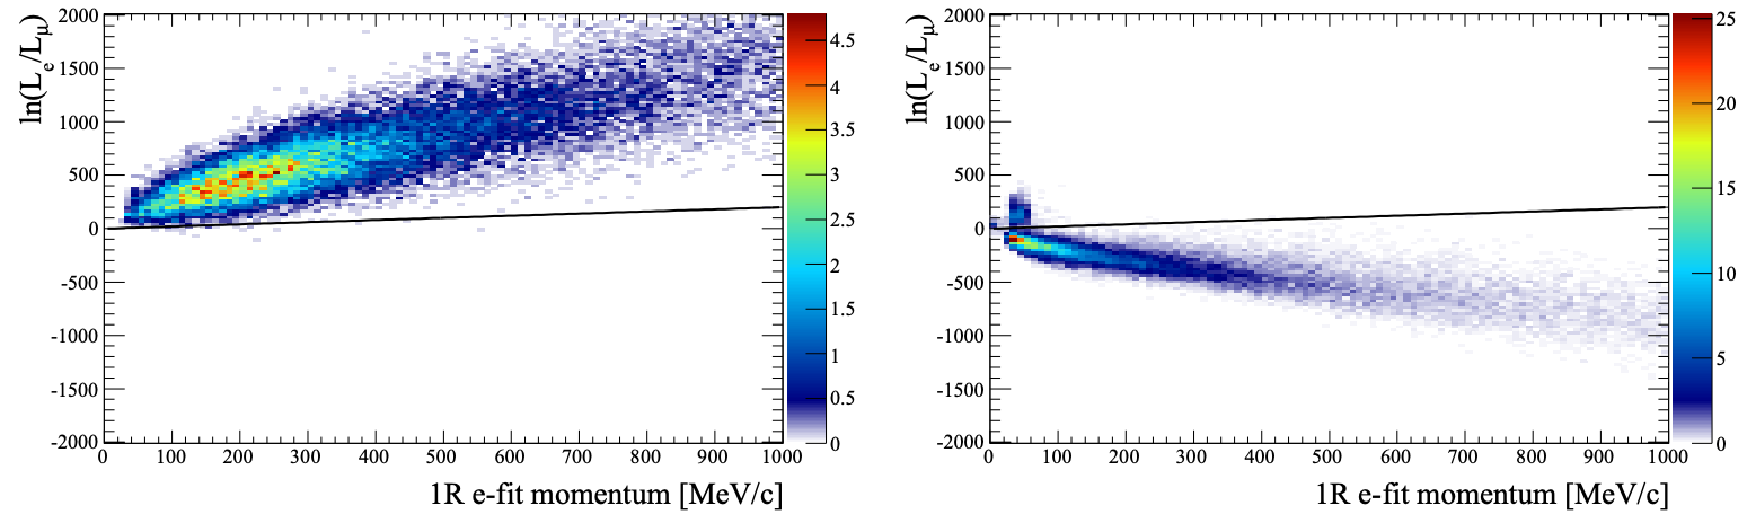
\includegraphics[width=\textwidth, trim={0mm 0mm 0mm 0mm}, clip, page=1]{Figures/Simulations/LogLikelihoodDiscriminator.pdf}
  \end{subfigure}
  \caption{The difference of the electron-like and muon-like log-likelihood compared to the reconstructed single-ring fit momentum for atmospheric \quickmath{\nu_{e}} (left) and \quickmath{\nu_{\mu}} (right) samples. The black line represents the cut used to discriminate electron-like and muon-like events, with coefficients obtained from Monte Carlo studies. Figures from \cite{t2k_tn_146}.}
  \label{fig:Simulations_LLHDiscriminator}
\end{figure}

\begin{figure}[h]
  \begin{subfigure}[t]{0.9\textwidth}
    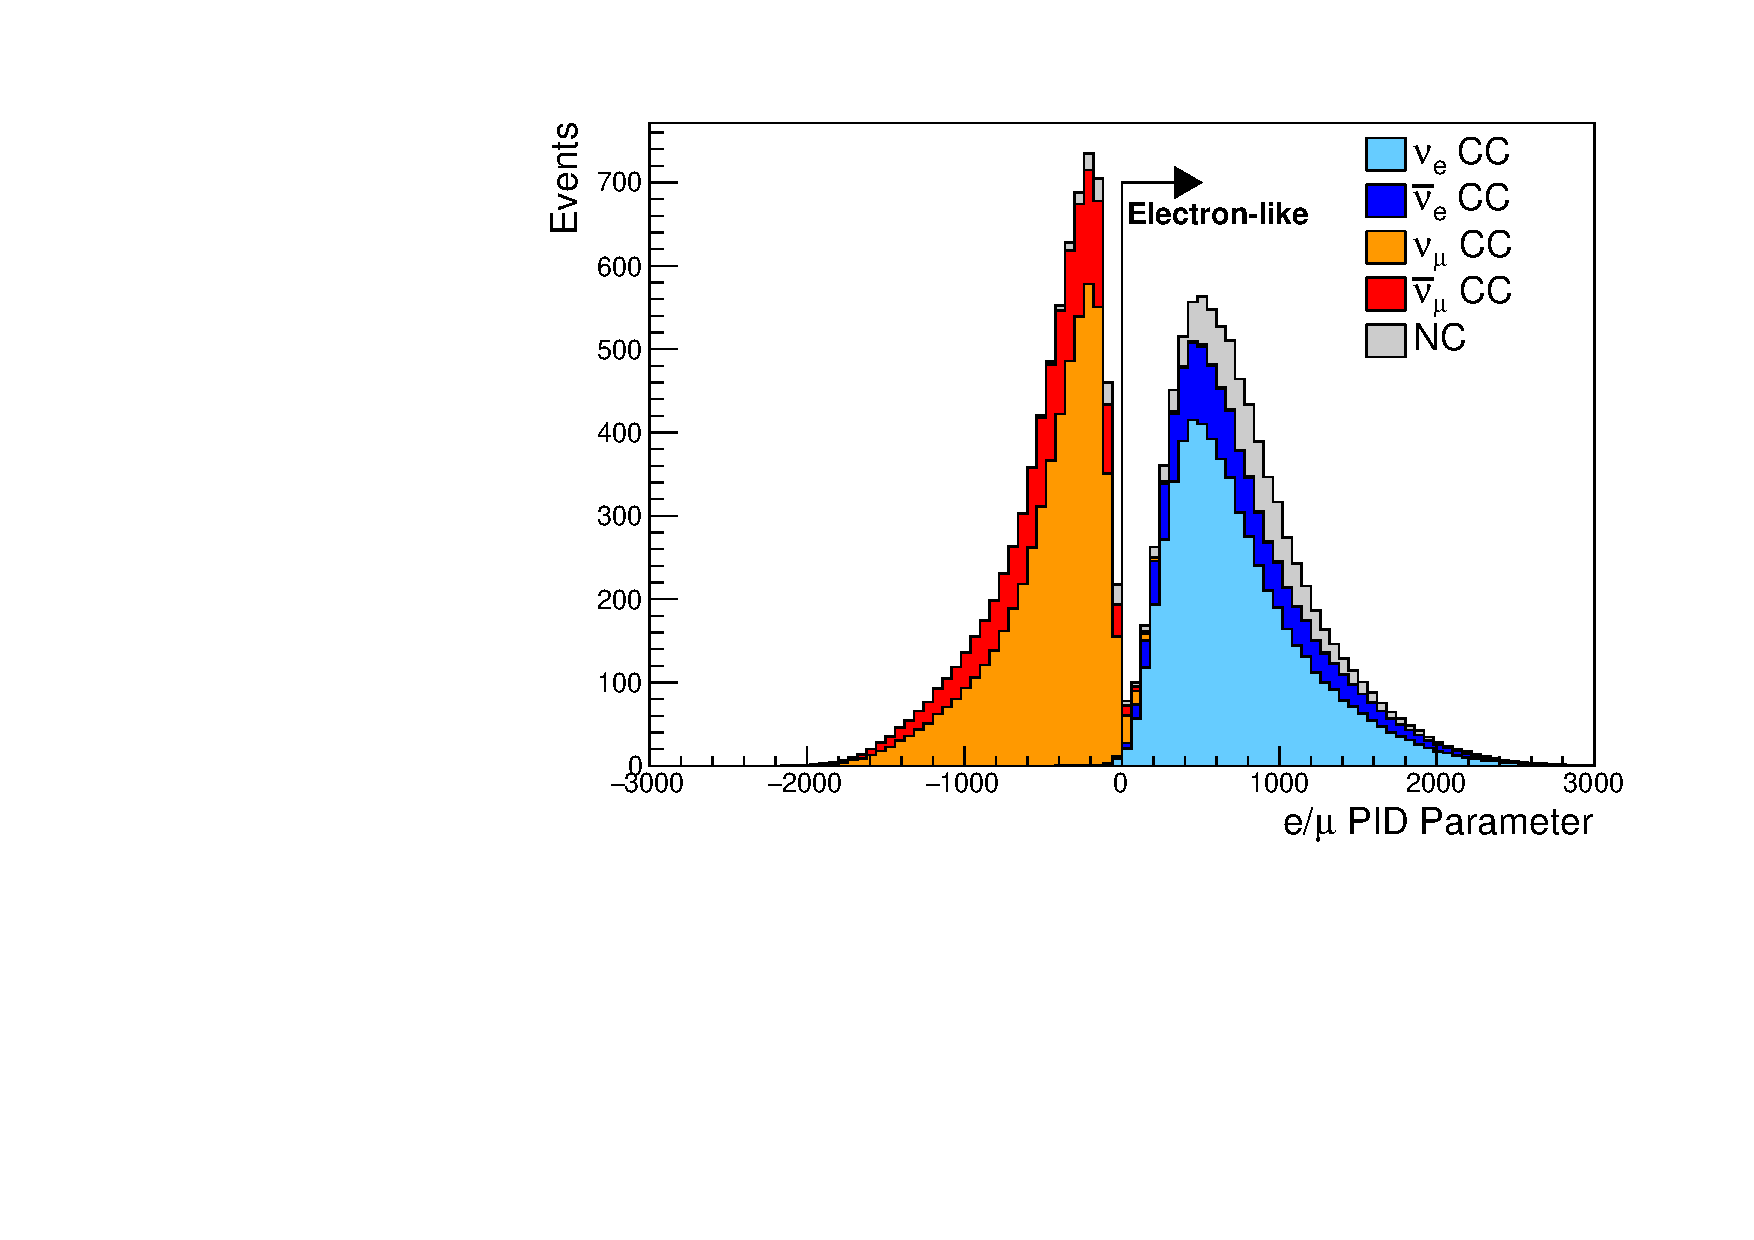
\includegraphics[width=\textwidth, trim={0mm 0mm 0mm 0mm}, clip, page=1]{Figures/Simulations/PIDParameter.pdf}
  \end{subfigure}
  \caption{The electron/muon PID separation parameter for all sub-GeV single-ring events in SK-IV. The charged current (CC) component is broken down in four flavours of neutrino (\quickmath{\nu_{\mu}}, \quickmath{\bar{\nu}_{\mu}}, \quickmath{\nu_{e}} and \quickmath{\bar{\nu}_{e}}). Events with positive values of the parameter are determined to be electron-like.}
  \label{fig:Simulations_EMUPIDParamDistribution}
\end{figure}

The \texttt{fiTQun} algorithm also considers a \quickmath{\pi^{0}} hypothesis. To do this, it performs a fit looking for two standard electron-hypothesis tracks which point to the same four-vertex. This assumes the electron tracks are generated from photon-conversion so the electron tracks actually appear offset from the proposed \quickmath{\pi^{0}} vertex. For these fits, the conversion length, direction, and momentum of each photon are also considered as track parameters which are then fit in the same methodology as the standard single-ring hypotheses. 

Whilst lower energy events are predominantly single-ring events, higher energy neutrino events can generate final states with multiple particles which generate Cherenkov photons. These ``multi-ring'' hypotheses are also considered in the \texttt{fiTQun} algorithm. When calculating the charge likelihood density, the predicted charge associated with each ring is calculated separately and then summed to calculate the total accumulated charge on each PMT. Similarly, the time likelihood for the multi-ring hypothesis is calculated assuming each ring is independent. Each track is time-ordered based on the time of flight from the center of the track to the PMT and the direct light from any ring incident on the PMT is assumed to arrive before any scattered light. To reduce computational resource usage, the multi-ring fits only consider electron-like and charged pion-like rings as the pion fit can be used as a proxy for a muon fit due to their similar mass. Due to the pions ability to interact through the strong force, they are more likely to hard-scatter. That means a single charged pion can produce multiple rings in different directions. There is an additional freedom, the fraction of kinetic energy lost in a single ring segment, which is added into the \texttt{fiTQun} pion fit to cover this difference. Pion and muon rings are indistinguishable when this fraction tends to unity.

Multi-ring fits proceed by proposing another ring to the previous fit and then fitting the parameters in the method described above. Typically, multi-ring fits have the largest likelihood because of the additional degrees of freedom introduced. A likelihood value is calculated for the \quickmath{n}-ring and \quickmath{(n+1)}-ring hypotheses, where the additional ring is only included if the likelihood value is above \quickmath{9.35}, based on Monte Carlo studies in \cite{Tobayama:2016dsi}.

\subsection{Validation of Reconstruction in SK-V}
\label{sec:Simulation_ReconstructionInSKV}

Understanding how the modeling of the detector conditions and stability affects the reconstruction is critical for ensuring accurate measurements. It is important to note that the detector systematics used in the 2020 T2K-only \cite{Dunne2020-uf} oscillation analysis are determined using data-to-Monte Carlo comparisons of the SK-IV data \cite{t2k_tn_399}. Due to tank-open maintenance occurring between SK-IV and SK-V, the dark rate of each PMT was observed to increase in SK-V due to light exposure for a significant time during the repairs. This increase can be seen in \autoref{fig:Simulations_DarkRateVariation}. Run-10 of the T2K experiment was conducted in the SK-V period, so the consistency of SK-IV and SK-V data needs to be studied to determine whether the SK-IV-defined systematics can be applied to the run-10 data. Consequently, the author of this thesis assessed the quality of \texttt{fiTQun} event reconstruction for SK-V data.

This comparison study was performed using the stopping muon data set for both the SK-IV and SK-V periods. This data sample is used due to the high rate of interactions as well as having similar energies to muons from CCQE \quickmath{\nu_{\mu}} interactions from beam interactions. The rate of cosmic muons does depend on the solar activity cycle \cite{Maghrabi2021} but this effect has been neglected in this comparison study. This is because the shape of the distributions is most important for the purposes of being compared to the detector systematics. The SK-IV and SK-V data samples consist of \quickmath{2398.42} and \quickmath{626.719} hours of data which equates to \quickmath{686\text{k}} and \quickmath{192\text{k}} events respectively. These samples do not amount to the full data sets of either period but do contain enough events to be systematics limited rather than statistics limited.

\begin{figure}[h]
  \begin{subfigure}[t]{\textwidth}
    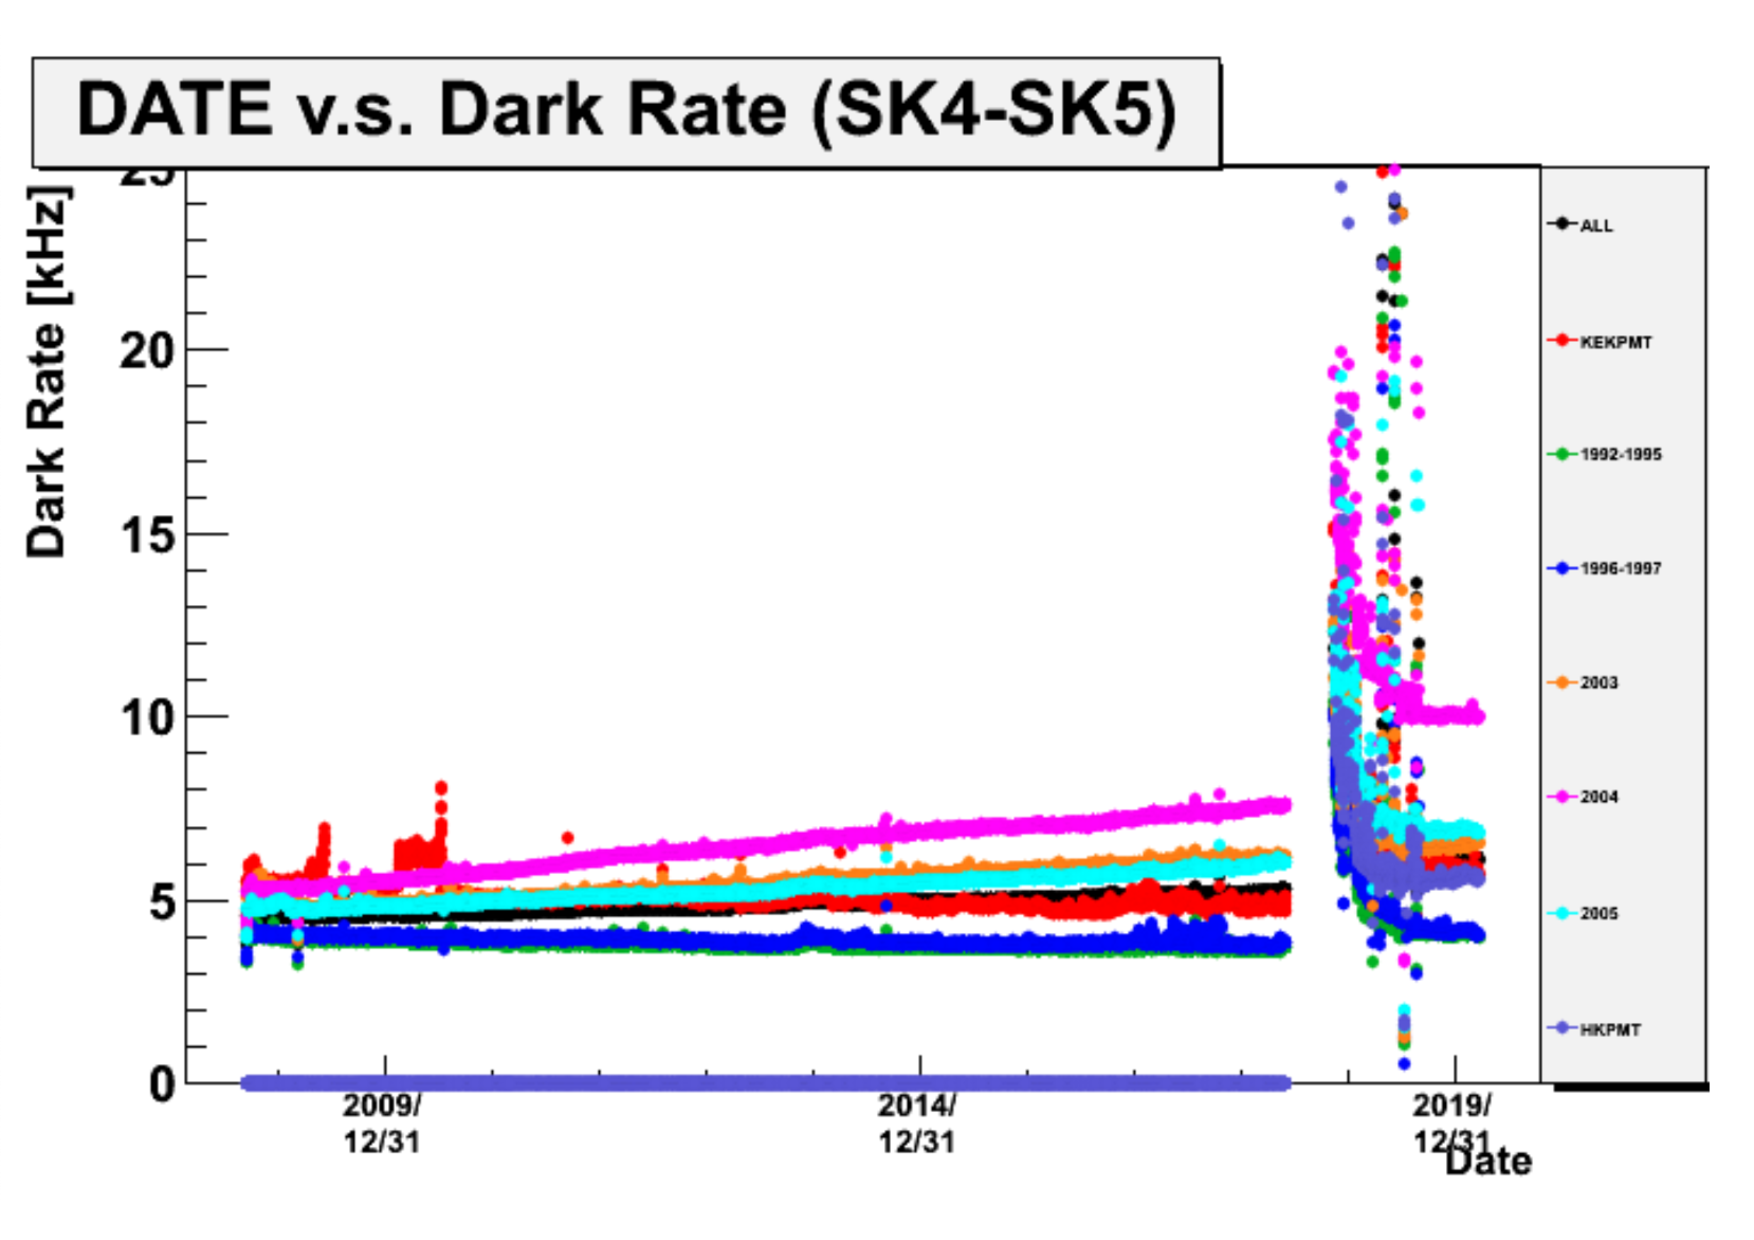
\includegraphics[width=\textwidth, trim={0mm 0mm 0mm 0mm}, clip, page=1]{Figures/Simulations/DarkRate.pdf}
  \end{subfigure}
  \caption{The variation of the measured dark rate as a function of date, broken down by PMT type. The SK-IV and SK-V periods span September 2008 to May 2018 and January 2019 to July 2020, respectively. The break in measurement in 2018 corresponds to the period of tank repair and refurbishment. Figure adapted from \cite{t2k_tn_399}.}
  \label{fig:Simulations_DarkRateVariation}
\end{figure}

The predicted charge calculated in the \texttt{fiTQun} algorithm includes a contribution from the photoelectron emission due to dark noise. Therefore, the increase in the SK-V dark rate needs to be accounted for. In practice, the average dark rate in each SK period is calculated and used as an input in the reconstruction. This is calculated by averaging the dark rate per run for each period separately, using the calibration measurements detailed in \autoref{subsec:T2KSKExp_SKCalibration}. The average dark rate from SK-IV and SK-V were found to be \quickmath{4.57\text{kHz}} and \quickmath{6.30\text{kHz}}, respectively. The charges associated with the muon and decay electron subevents are illustrated in \autoref{fig:Simulations_MeasuredChargeDistribution}. The photoelectron emission from dark noise is more significant for events that have lower energy. This is because this contribution becomes more comparable to the number of photoelectrons emitted from incident photons in lower-energy events. This behaviour is observed in the data, where the charge deposited by the muon subevent is mostly unaffected by the increase in dark rate, whilst the charge associated with the decay-electron is clearly affected.

\begin{figure}[h]
  \begin{subfigure}[t]{0.48\textwidth}
    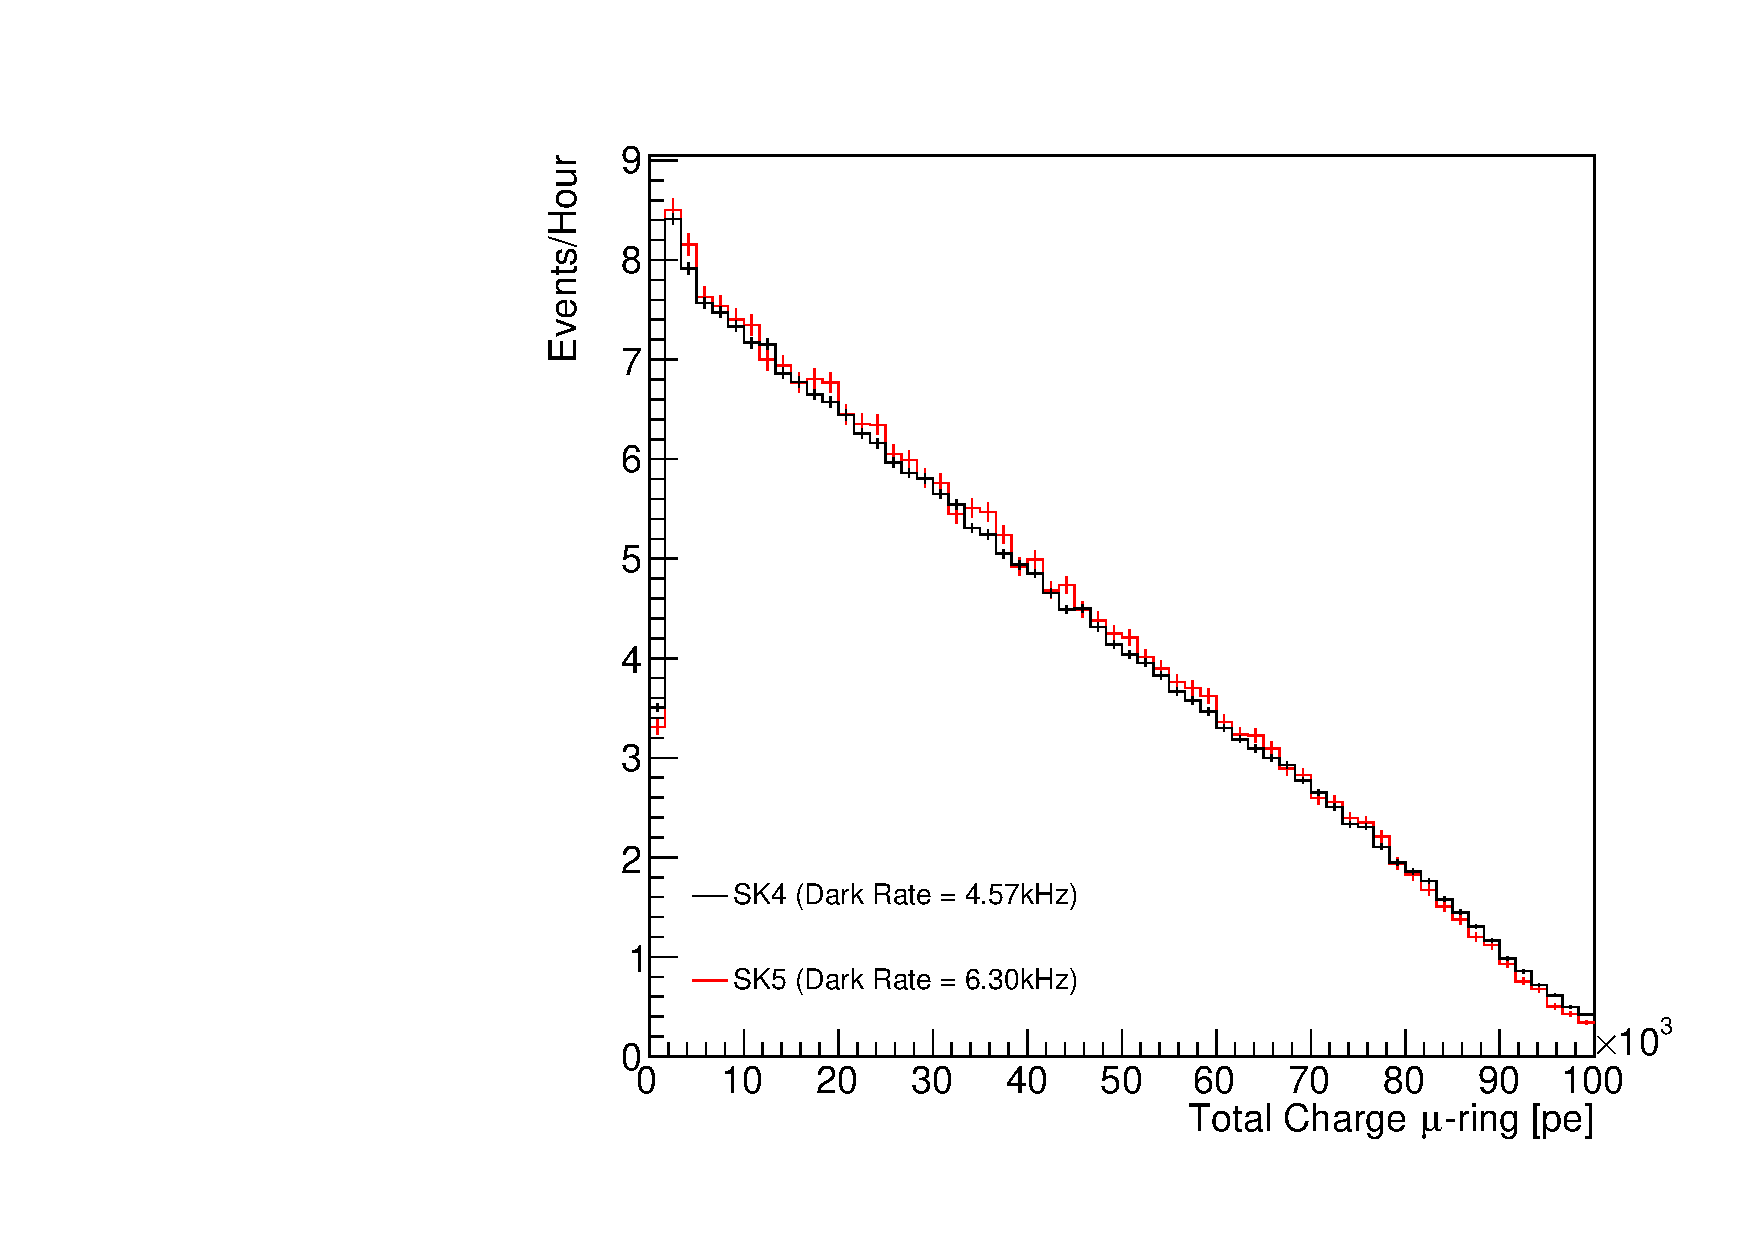
\includegraphics[width=\textwidth, trim={0mm 0mm 0mm 0mm}, clip, page=1]{Figures/Simulations/ChargeAssociatedWithMuon.pdf}
    \subcaption{Muon}
  \end{subfigure}%
  \begin{subfigure}[t]{0.48\textwidth}
    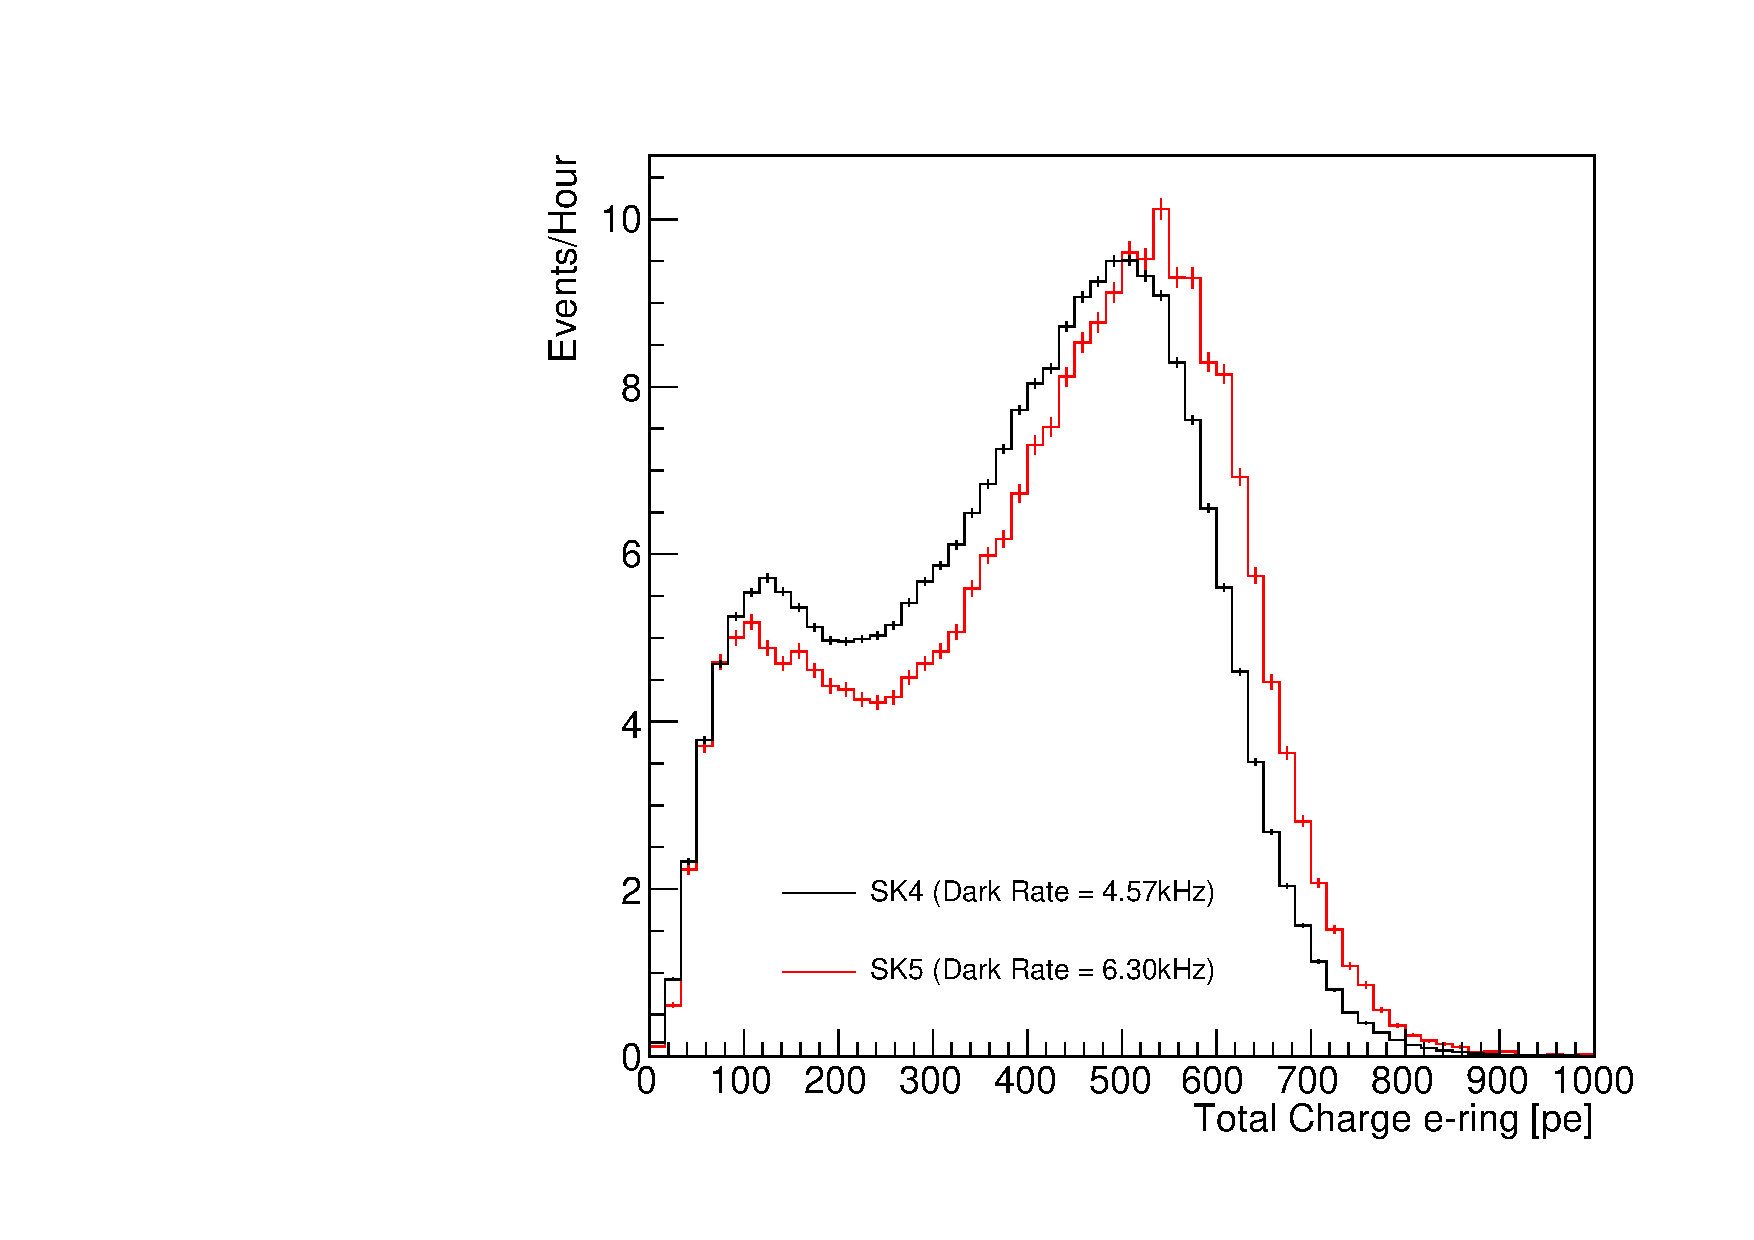
\includegraphics[width=\textwidth, trim={0mm 0mm 0mm 0mm}, clip, page=1]{Figures/Simulations/ChargeAssociatedWithDecayE.pdf}
    \subcaption{Decay Electron}
  \end{subfigure}  
  \caption{Comparison of the measured raw charge deposited per event from the stopping muon data samples between SK-IV (Black) and SK-V (Red), split by the primary muon subevent (left) and the associated decay electron subevent (right).}
  \label{fig:Simulations_MeasuredChargeDistribution}
\end{figure}

The energy scale systematic is estimated from data-to-Monte Carlo differences in the stopping muon sample in \cite{Kamiokande_Collaboration2017-nf} and found to be \quickmath{2.1\%}. To determine the consistency of SK-IV and SK-V with respect to the energy scale systematic, the muon momentum distribution is compared between the two SK periods. As the total number of Cherenkov photons is integrated across the track length, the reconstructed momentum divided by track length (or range) is compared between SK-IV and SK-V as illustrated in \autoref{fig:Simulations_MuonMomentumByRange}.

\begin{figure}[h]
  \begin{subfigure}[t]{\textwidth}
    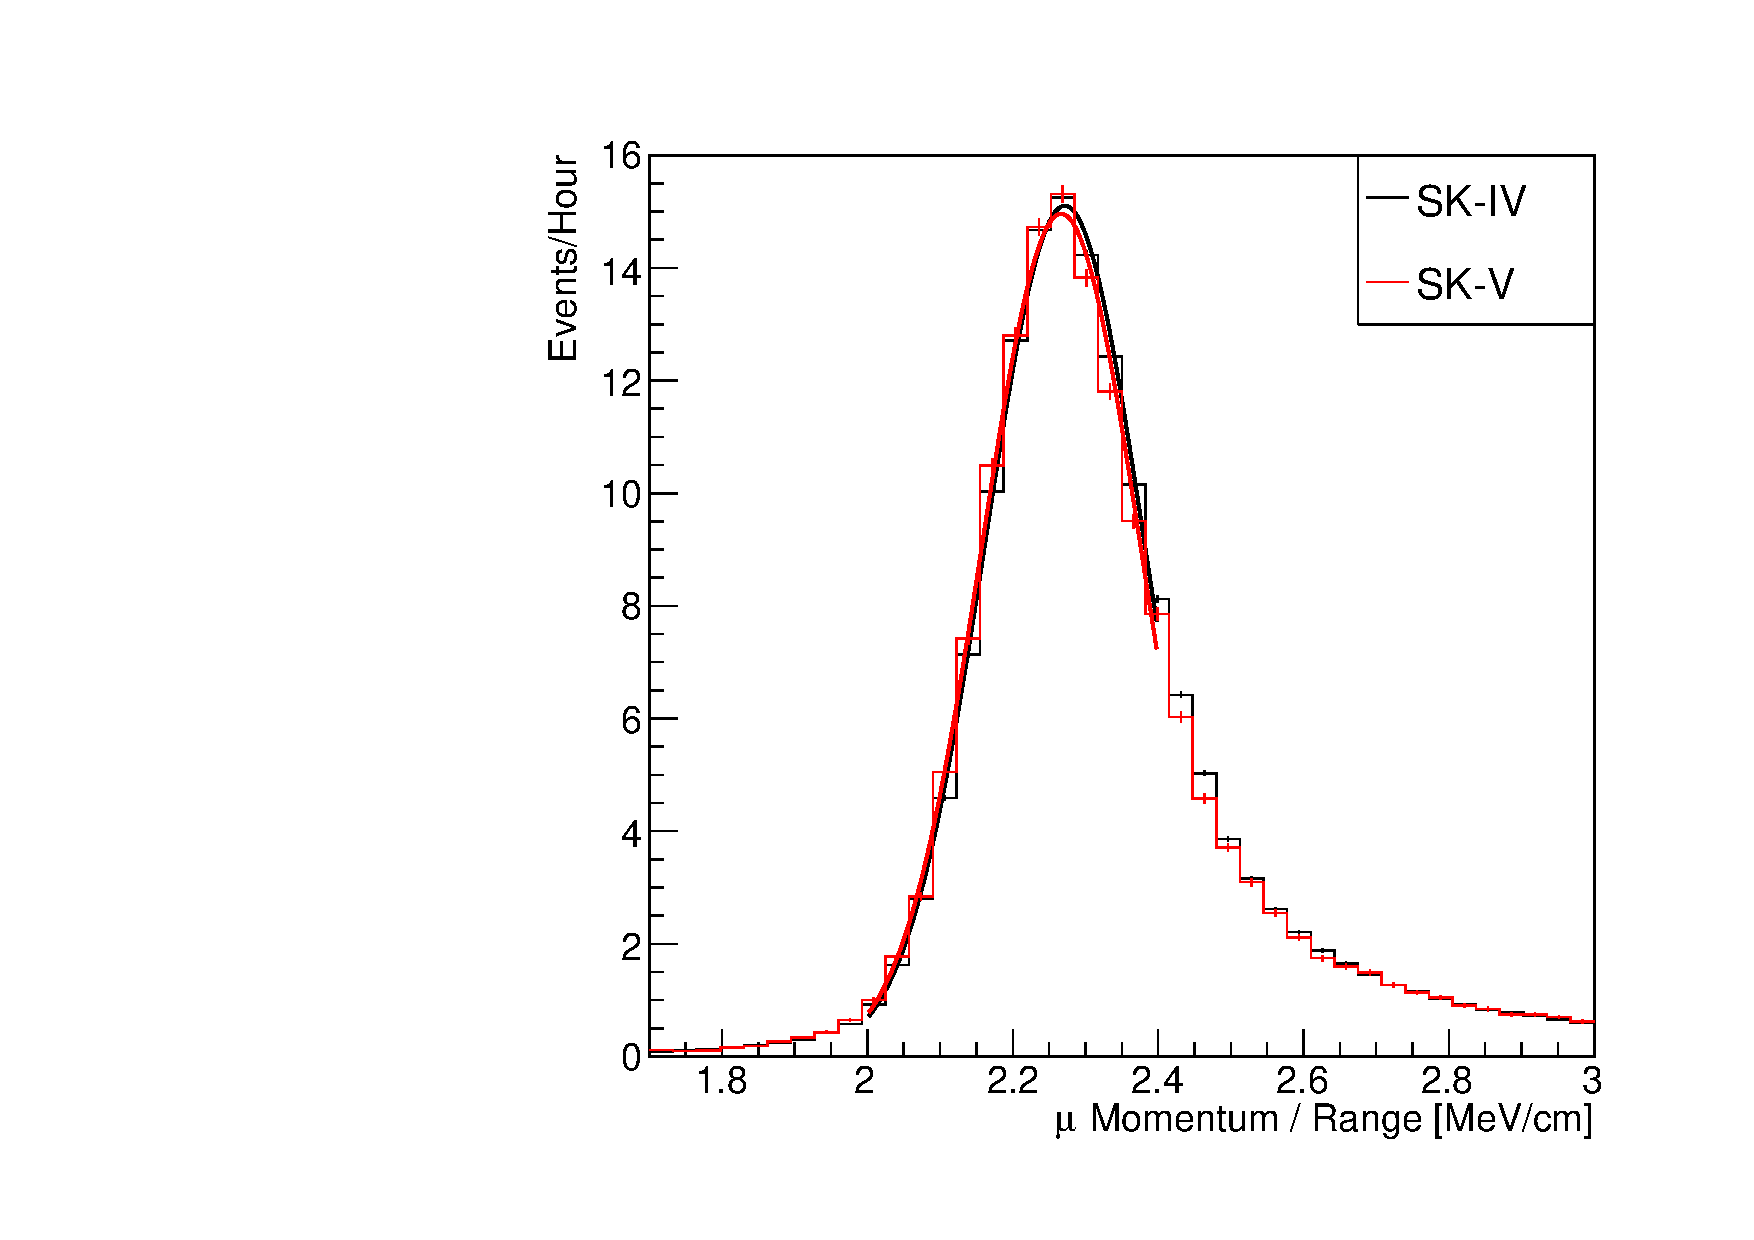
\includegraphics[width=\textwidth, trim={0mm 0mm 0mm 0mm}, clip, page=1]{Figures/Simulations/MuonRangeComparison.pdf}
  \end{subfigure}
  \caption{The distribution of the reconstructed momentum from the muon ring divided by the distance between the reconstructed muon and decay electron vertices as found in the stopping muon data sets of SK-IV (Black) and SK-IV (Red). Only events with one tagged decay electron are considered. A Gaussian fit is considered in the range \quickmath{[2.0,2.4] \text{MeV/cm}} and illustrated as the solid curve.}
  \label{fig:Simulations_MuonMomentumByRange}
\end{figure}

The consistency between these muon distributions has been computed in two ways. Firstly, a Gaussian is fit to the peak of each distribution separately, whose mean is found to be \quickmath{(2.272 \pm 0.003) \text{MeV/cm}} and \quickmath{(2.267 \pm 0.006) \text{MeV/cm}} for SK-IV and SK-V respectively. The ratio of these is equal to \quickmath{1.002 \pm 0.003}. The means of the Gaussian fits are consistent with the expected stopping power of a minimum ionising muon for a target material (water) with \quickmath{Z/A \sim 0.5} \cite{PhysRevD.86.010001}. The second consistency check is performed by introducing a nuisance parameter, \quickmath{\alpha}, which modifies the SK-V distribution. The value of \quickmath{\alpha} which minimises the \quickmath{\chi^{2}} value between the SK-IV and SK-V is determined by scanning across a range of values. This is repeated by applying the nuisance parameter as both a multiplicative factor and an additive shift. The \quickmath{\chi^{2}} distributions for different values of \quickmath{\alpha} is illustrated in \autoref{fig:Simulations_MuonMomentumByRangeChi2Scan}. The values which minimise the \quickmath{\chi^{2}} are found to be \quickmath{0.0052} and \quickmath{1.0024} for the additive and multiplicative implementations, respectively. No evidence of shifts larger than the \quickmath{2.1\%} uncertainty on the energy scale systematic has been found in the reconstructed momentum distribution of SK-IV and SK-V.

\begin{figure}[h]
  \begin{subfigure}[t]{\textwidth}
    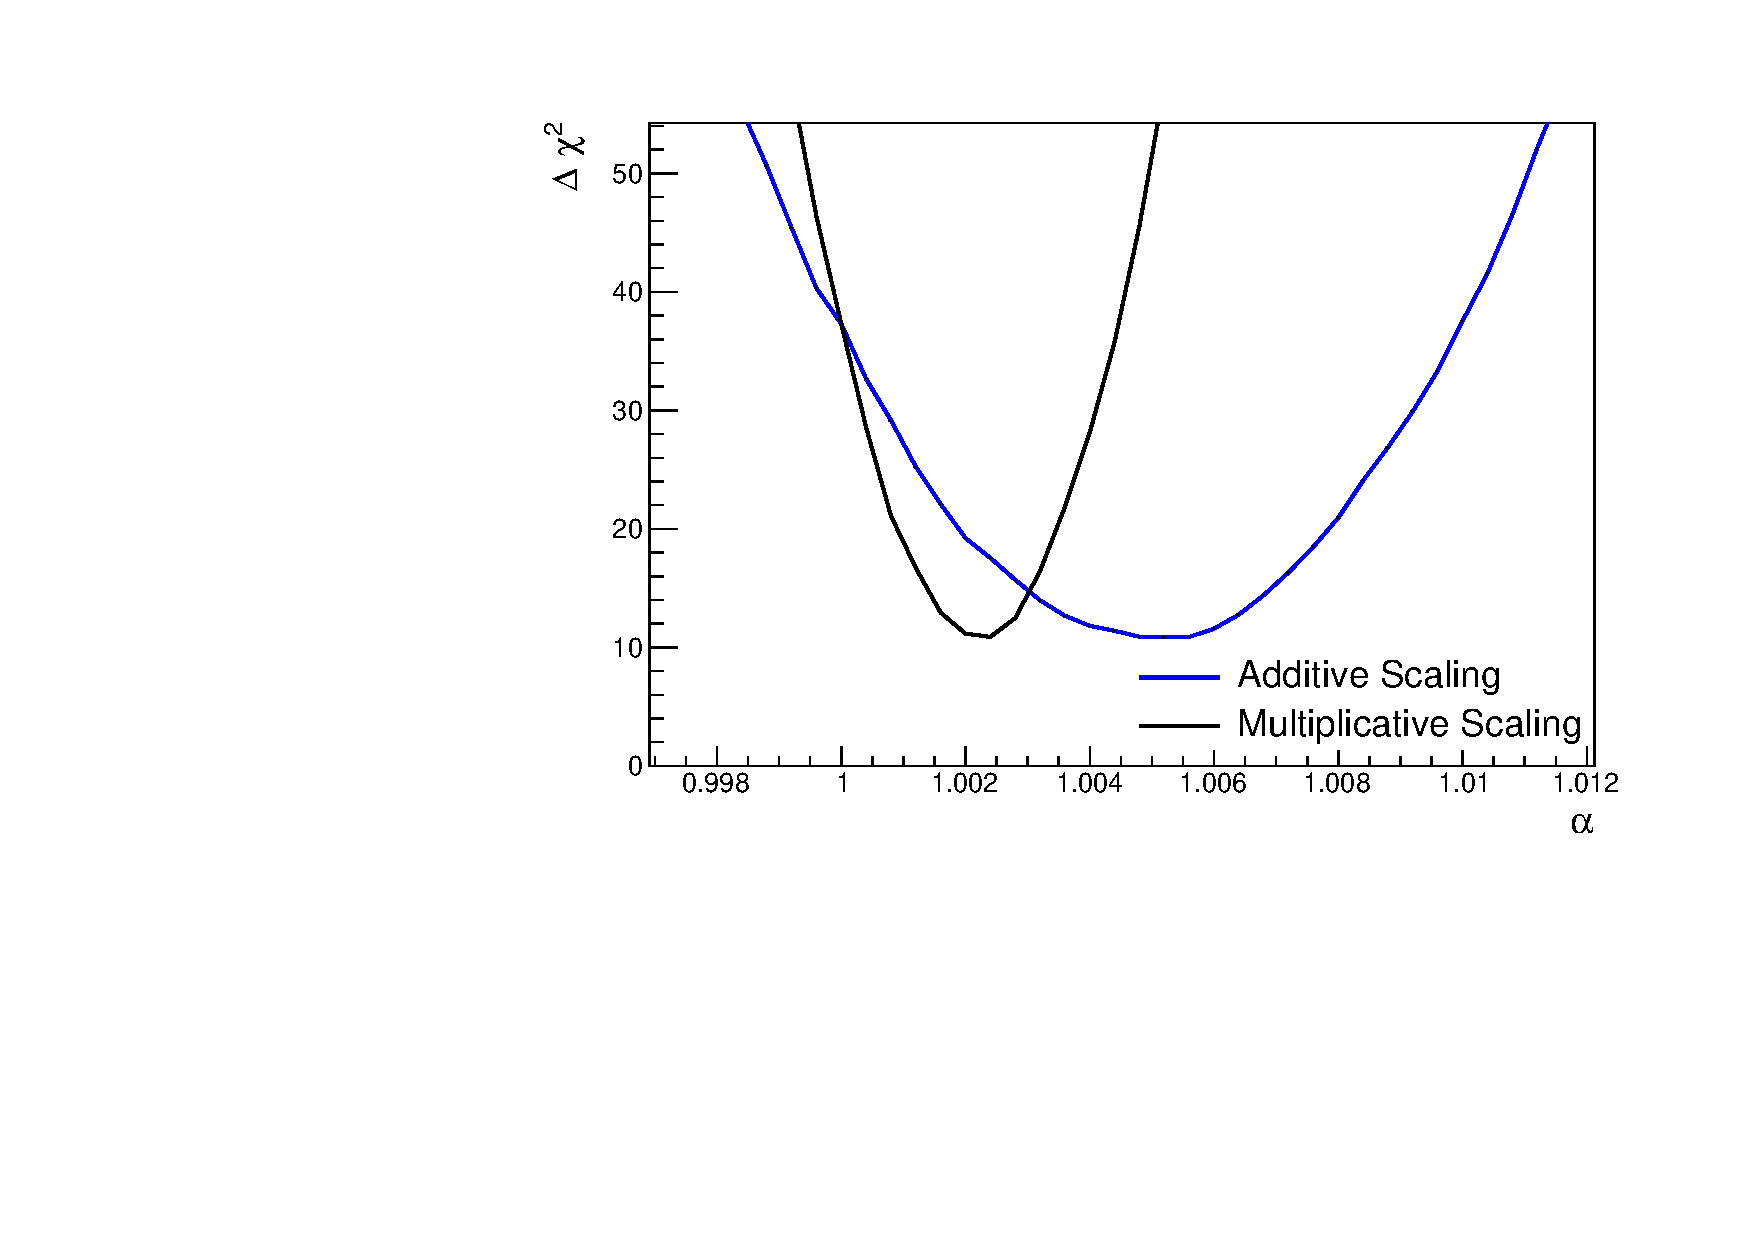
\includegraphics[width=\textwidth, trim={0mm 0mm 0mm 0mm}, clip, page=1]{Figures/Simulations/MuonRange_Chi2Scan.pdf}
  \end{subfigure}
  \caption{The \quickmath{\chi^{2}} difference between the SK-IV and SK-V reconstructed muon momentum divided by range when the SK-V is modified by the scaling parameter \quickmath{\alpha}. Both additive (Blue) and multiplicative (Black) scaling factors have been considered. In practice, the additive scaling factor actually uses the value of (\quickmath{\alpha-1.0}) but is illustrated like this so the results can be shown on the same axis range.}
  \label{fig:Simulations_MuonMomentumByRangeChi2Scan}
\end{figure}

\section{Event Reduction at SK}
\label{sec:Simulations_Reduction}

In normal data-taking operations, the SK detector observes many background events alongside the beam and atmospheric neutrino signal events of physics interest for this thesis. Cosmic ray muons and flasher events, which are the spontaneous discharge of a given PMT, contribute the largest amount of background events in the energy range relevant to this thesis.
%Lower energy analyses like DSNB searches are also subject to radioactive backgrounds \cite{Nakano_2017}.
Therefore the data recorded is reduced with the aim of removing these background events. The reduction process is detailed in \cite{Ashie_2005, Jiang2019-iw} and briefly summarised below.

Atmospheric neutrino events observed in the SK detector are categorised into three different types of samples: fully contained (FC), partially contained (PC) and up-going muon (Up-$\mu$), using PMT hit signatures in the inner and outer detector (ID and OD, respectively). To identify FC neutrino events, it is required that the neutrino interacts inside the fiducial volume of the ID and that no significant OD activity is observed. For this analysis, an event is defined to be in the fiducial volume provided the event vertex is at least $0.5$m away from the ID walls. PC events have the same ID requirements but can have a larger signal present inside the OD. Typically, only high energy muons from \quickmath{\nu_{\mu}} interactions can penetrate the ID wall. The Up-$\mu$ sample contains events where muons are created from neutrino interactions in the OD water or rock below the tank. They then propagate upwards through the detector. Downward-going muons generated from neutrino interactions above the tank are neglected because of the difficulty in separating their signature from the cosmic muon shower background. The sample categories are visually depicted in Figure \ref{fig:Simulations_AtmosphericSampleTopology}.

\begin{figure}[ht!]
    \centering
    \includegraphics[width=0.8\textwidth]{Figures/Simulations/Atmo_topology.pdf}
    \caption{A depiction of the topology patterns for fully-contained (FC), partially-contained (PC), and up-going muon (\quickmath{\text{Up-}\mu}) samples included in this analysis.}
    \label{fig:Simulations_AtmosphericSampleTopology}
\end{figure}

Based on the event characteristics, as defined by the \texttt{fiTQun} event reconstruction software, the FC events are categorised by

\begin{itemize}
    \item \textbf{Visible Energy}: equal to the sum of the reconstructed kinetic energy of particles above the Cerenkov threshold for all rings present in the event. The purpose is to separate events into sub-GeV and multi-GeV categories. 
    \item \textbf{Number of observed Cerenkov rings}. The purpose is to separate single-ring and multi-ring events, where single-ring events predominantly consist of quasi-elastic interactions and multi-ring events are typically resonant pion production or deep inelastic scattering events.
    \item \textbf{Particle identification parameter of the most energetic ring}: A value determined from the maximum likelihood value based on \texttt{fiTQun}'s electron, muon, or pion hypothesis. The purpose is to separate electron-like and muon-like events.
    \item \textbf{Number of decay electrons}: The purpose is to separate quasi-elastic events (which have one decay electron emitted from the muon decay) and resonant pion production events (which have two decay electrons emitted from the muon and pion).
\end{itemize}

The PC and \quickmath{\text{Up-}\mu} categories are broken down into ``through-going'' and ``stopping'' samples depending on whether the muon leaves the detector. This is because stopping events deposit the entire energy of the interaction into the detector, resulting in better reconstruction. The energy of events that exit the detector has to be estimated, with a typically worse resolution, which introduces much larger systematic uncertainties. Through-going \quickmath{\text{Up-}\mu} samples are further broken down by whether any hadronic showering was observed in the event which typically indicates DIS interactions. The expected neutrino energy for the different categories is given in \autoref{fig:Simulations_NeutrinoEnergyDistribution}. FC sub-GeV and multi-GeV events peak around \quickmath{0.7\text{GeV}} and \quickmath{3\text{GeV}} respectively, with slightly different peak energies for \quickmath{\nu_{e}} and \quickmath{\nu_{\mu}} oscillation channels. PC and \quickmath{\text{Up-}\mu} are almost entirely comprised of \quickmath{\nu_{\mu}} events and peak around \quickmath{7\text{GeV}} and \quickmath{100\text{GeV}}, respectively.

\begin{figure}[h]
  \begin{subfigure}[t]{0.49\textwidth}
    \includegraphics[width=\textwidth, trim={0mm 0mm 0mm 0mm}, clip,page=1]{Figures/Simulations/NeutrinoEnergyDist_NuE.pdf}
  \end{subfigure}%
  \begin{subfigure}[t]{0.49\textwidth}
    \includegraphics[width=\textwidth, trim={0mm 0mm 0mm 0mm}, clip,page=1]{Figures/Simulations/NeutrinoEnergyDist_NuMu.pdf}
  \end{subfigure}
  \begin{subfigure}[t]{0.49\textwidth}
    \includegraphics[width=\textwidth, trim={0mm 0mm 0mm 0mm}, clip,page=1]{Figures/Simulations/NeutrinoEnergyDist_NuTau.pdf}
  \end{subfigure}%
  \caption{The predicted neutrino flux of the fully contained (FC) sub-GeV and multi-GeV, partially contained (PC), and upward-going muon (\quickmath{\text{Up-}\mu}) events. The prediction is broken down by the \quickmath{\nu_{x} \rightarrow \nu_{e}} prediction (top left), \quickmath{\nu_{x} \rightarrow \nu_{\mu}} prediction (top right) and \quickmath{\nu_{x} \rightarrow \nu_{\tau}} prediction (bottom). \quickmath{\nu_{x}} represents the flavours of neutrinos produced in the cosmic ray showers (electron and muon). Asimov A oscillation parameters are assumed (given in \autoref{tab:Theory_ParameterSets}).}
  \label{fig:Simulations_NeutrinoEnergyDistribution}
\end{figure}

The first two steps in the FC reconstruction remove the majority of cosmic ray muons by requiring a significant amount of ID activity compared to that measured in the OD. Events that pass this cut are typically very high momentum muons or events that leave very little activity in the OD. Consequently, a third reduction step is then applied to select cosmic-ray muons that pass the initial reduction step. A purpose-built cosmic muon fitter is used to determine the entrance (or exit) position of the muon and a cut is applied to OD activity contained within \quickmath{8\text{m}} of this position. Flasher events are removed in the fourth reduction step which is based on the close proximity of PMT hits surrounding the PMT producing the flash. Events that pass all these reduction steps are reconstructed with the \texttt{APFit} algorithm. The fifth step of the reduction uses information from this more precise fitter to repeat the previous two steps with tighter cuts. Muons below the Cherenkov threshold can not generate optical photons in the ID but the associated decay electron can due to its lower mass. These are the types of events targeted in the fifth reduction step. The final cuts require the event vertex to be within the fiducial volume (\quickmath{0.5\text{m}} from the wall), visible energy \quickmath{E_{vis} > 30\text{MeV}} and fewer than 16 hits within the higher energy OD cluster. The culmination of the fully contained reduction results in \quickmath{8.09} events/day in the nominal fiducial volume \cite{thesis_miao}. The uncertainty in the reduction is calculated by comparing Monte Carlo prediction to data. The largest discrepancy is found to be \quickmath{1.3\%} in the fourth reduction step.

The PC and \quickmath{\text{Up-}\mu} events are processed through their own reduction processes detailed in \cite{Ashie_2005}. Both of these samples are reconstructed with the \texttt{APFit} algorithm rather than \texttt{fiTQun}. This is because the efficiency of reconstructing events that leave the detector has not been sufficiently studied for reliable systematic uncertainties with \texttt{fiTQun}. The PC and \quickmath{\text{Up-}\mu} samples acquire events at approximately \quickmath{0.66} and \quickmath{1.44} events/day.

Beam neutrinos events undergo the same reduction steps as FC events and are then subject to further cuts \cite{t2k_tn_027}. The GPS system that links the timing between the beam facility and SK needs to be operating correctly and there should be no activity within the detector in the previous \quickmath{100 \mu\text{s}} before the trigger. The events then need to triggered between \quickmath{-2 \mu\text{s}} and \quickmath{10\mu\text{s}} of the expected spill timing.

The beam neutrino samples are not split by visible energy since their energy range is smaller than the atmospheric neutrino events. Following the T2K analysis in \cite{Dunne2020-uf}, only single-ring beam neutrino events are considered. Similar to atmospheric event selection, the number of decay electrons is used as a proxy for distinguishing CCQE and CCRES events. The expected neutrino energy, broken down by the number of decay electrons, is given in \autoref{fig:Simulations_NeutrinoEnergyDistribution_T2K}.

\begin{figure}[h]
  \begin{subfigure}[t]{0.49\textwidth}
    \includegraphics[width=\textwidth, trim={0mm 0mm 0mm 0mm}, clip,page=1]{Figures/Simulations/NeutrinoEnergyDist_T2K_NuE.pdf}
  \end{subfigure}%                                                                                                                                                                                         
  \begin{subfigure}[t]{0.49\textwidth}
    \includegraphics[width=\textwidth, trim={0mm 0mm 0mm 0mm}, clip,page=1]{Figures/Simulations/NeutrinoEnergyDist_T2K_NuMu.pdf}
  \end{subfigure}
  \caption{The predicted flux of beam neutrinos, as a function of neutrino energy. The predictions are broken down by the number of decay electrons associated with the particular events. Asimov A oscillation parameters are assumed (given in \autoref{tab:Theory_ParameterSets}).}
  \label{fig:Simulations_NeutrinoEnergyDistribution_T2K}
\end{figure}

\chapter{Sample Selections and Systematics}
\label{chap:SelsAndSysts}

The oscillation analysis presented within this thesis is built upon a simultaneous fit to atmospheric data at SK, neutrino beam data in the near detector, and beam data measured at SK. The definitions of these samples are documented in \autoref{sec:SelsAndSysts_Sels_Atms}, \autoref{sec:SelsAndSysts_Sels_ND}, and \autoref{sec:SelsAndSysts_Sels_FD}, respectively. The data collected and used within this analysis is detailed in \autoref{tab:SelsAndSysts_Sels_DataTotal}. The near and far detector data corresponds to T2K runs 2-9 and runs 1-10, respectively. The accumulated POT and beam power for runs \quickmath{1-10} are illustrated in \autoref{fig:SelsAndSysts_Beam_PowerAndPOT}.

\begin{table}[ht!]
    \centering
    \begin{tabular}{l|c}
      \hline
      Data Type & Total \\
      \hline
      Near Detector FHC & \quickmath{1.15 \times 10^{21}}POT \\
      Near Detector RHC & \quickmath{8.34 \times 10^{20}}POT \\
      Far Detector FHC & \quickmath{1.97 \times 10^{21}}POT \\
      Far Detector RHC & \quickmath{1.63 \times 10^{21}}POT \\
      Atmospheric SK-IV & \quickmath{3244.4} days \\
      \hline
      \hline
    \end{tabular}
    \caption{The amount of data collected in each detector used within this analysis. The data collected at the near and far detector, for both neutrino beam (FHC) and antineutrino beam (RHC), is measured as the number of protons on target (POT).}
    \label{tab:SelsAndSysts_Sels_DataTotal}
\end{table}

The difference in POT recorded at the near and far detector is due to the difference in downtime. The SK detector is very stable with almost \quickmath{100\%} of data recorded during beam operation. Due to various technical and operational issues, the downtime of the near detector is significantly higher due to its more complex design and operating requirements.

The systematic parameters invoked within the flux, detector, and interaction models used within this analysis are documented in \autoref{sec:SelsAndSysts_Systs}. The standard configuration of the joint beam and atmospheric data fit utilises far detector systematics provided in the official inputs from the two experiments. Additionally, a correlated detector model which fits the parameters used in sample selections to data has been developed and documented in \autoref{sec:SelsAndSysts_Systs_FD}.

\begin{figure}[h]
  \begin{subfigure}[t]{\textwidth}
    \includegraphics[width=\textwidth, trim={0mm 0mm 0mm 0mm}, clip,page=1]{Figures/Selections/BeamPowerAndPOT.pdf}
  \end{subfigure}
  \caption{The accumulated beam data, measured as the number of protons on target (POT). The total data (blue) is given which comprises of the neutrino beam (red) and antineutrino (purple) components. The beam power for neutrino and antineutrino beams is given as the markers using the same colour scheme. The timescale runs from Run 1 which started in January 2010 until Run 10 which ended in February 2020. The ratio of accumulated data in neutrino and antineutrino beam is \quickmath{54.7\%:45.3\%}.}
  \label{fig:SelsAndSysts_Beam_PowerAndPOT}
\end{figure}

\finish{Say that I have merged T2K and SK which hadn't previously been done}

\newpage
\section{Atmospheric Samples}
\label{sec:SelsAndSysts_Sels_Atms}

The atmospheric event selection follows the official SK-IV analysis presented in \cite{Jiang2019-iw} and is documented below. The Monte Carlo prediction used within this analysis corresponds to \quickmath{500} years worth of neutrino events, which is scaled down to match the SK-IV livetime of \quickmath{3244.4} days.

The fully contained (FC), partially contained (PC), and upward going muon events (up-\quickmath{\mu}) which pass the reduction cuts discussed in \autoref{sec:Simulations_Reduction} are further broken down into different samples based on reconstruction information. This section details the samples used within this oscillation analysis, alongside the chosen binning.

FC events are first separated by the visible energy deposited within the detector. This is calculated as the sum of the reconstructed kinetic energy above the Cherenkov threshold for all rings present in the event. Events are separated by whether they were above or below \quickmath{E_{vis} = 1.33\text{GeV}}. This separates ``subGeV'' and ``multiGeV'' events. Typically, lower energy events consist of charged current quasi-elastic (CCQE) interactions which are better understood and simpler to reconstruct resulting in smaller systematic uncertainties. Events are further separated by the number of rings associated with the event due to similar reasoning. As the oscillation probability is dependant upon the flavour of neutrino, electron and muon events are separated using a similar likelihood method to that discussed in \autoref{sec:Simulation_Reconstruction}. To reduce computational resources required for the reconstruction, only electron and pion hypotheses are considered so this separation cut depends on the ratio of the electron to pion likelihoods, \quickmath{\log(L_{e}/L_{\pi})}. Finally, the number of decay electrons is used to classify events. Charged current resonant pion production (CCRES) interactions generate a final-state pion. This can decay, mostly likely through a muon, into a decay electron. Therefore any electron-like event with one decay electron or muon-like event with two decay electrons was most likely produced by a CCRES interaction. Consequently, the number of decay electrons can be used to distinguish CCQE and CCRES interaction modes. Ultimately, FC subGeV events are separated into the samples listed in \autoref{tab:SelsAndSysts_Sels_Atms_SubGeV}.

\begin{table}[ht!]
    \centering
    \begin{tabular}{c|l}
      \hline
      Sample Name & Description \\
      \hline
      \texttt{SubGeV-elike-0dcy} & Single ring \quickmath{e}-like events with zero decay electrons \\ \hline
      \texttt{SubGeV-elike-1dcy} & Single ring \quickmath{e}-like events with one or more decay electrons \\ \hline
      \texttt{SubGeV-mulike-0dcy} & Single ring \quickmath{\mu}-like events with zero decay electrons \\ \hline
      \texttt{SubGeV-mulike-1dcy} & Single ring \quickmath{\mu}-like events with one decay electrons \\ \hline
      \texttt{SubGeV-mulike-2dcy} & Single ring \quickmath{\mu}-like events with two or more decay electrons \\ \hline
      \texttt{SubGeV-pi0like} & Two \quickmath{e}-like ring events with zero decay electrons \\
      & \hspace{0.2cm} and reconstructed \quickmath{\pi^{0}} mass \quickmath{85 \leq m_{\pi^{0}} < 215 \text{MeV}} \\
      \hline
      \hline
    \end{tabular}
    \caption{The fully contained subGeV samples, defined as events with visible energy\quickmath{E_{vis} < 1.33\text{GeV}}, used within this oscillation analysis.}
    \label{tab:SelsAndSysts_Sels_Atms_SubGeV}
\end{table}

In addition to the cuts discussed above, multiGeV samples also have additional cuts to separate samples which target neutrino and antineutrino events. As discussed in \autoref{sec:Oscillation_Overview}, the matter resonance only occurs for neutrinos in  the normal hierarchy and antineutrinos in the inverted mass hierarchy. Therefore, having flavour-enriched samples aids in the determination of the mass hierarchy. For a CCRES interaction,

\begin{align}
  \begin{split}
    \bar{\nu}_e + N \rightarrow e^{+} + N^{'} + &\pi^{-}, \\
    \nu_e + N \rightarrow e^{-} + N^{'} + &\pi^{+} \\
    &\hspace{5pt} \rotatebox[origin=c]{180}{$\Lsh$} \hspace{5pt} \mu^{+} + \nu_\mu \\
    &\hspace{20pt} \rotatebox[origin=c]{180}{$\Lsh$} \hspace{5pt} e^{+} + \nu_e + \bar{\nu}_\mu.
\end{split}
\end{align}

The \quickmath{\pi^{-}} emitted from a \quickmath{\bar{\nu_{e}}} interaction is more likely to be captured by an oxygen nucleus than the \quickmath{\pi^{+}} from \quickmath{\nu_{e}} interactions \cite{LeeKaPik}. These pions then decay, mostly through muons, to electrons. Therefore the number of tagged decay electrons associated with an event gives an indication of whether the interaction was due to a neutrino or antineutrino: zero for \quickmath{\bar{\nu}_{e}} events, and one for \quickmath{\nu_{e}} events. The ability to separate neutrino from antineutrino events is illustrated in \autoref{tab:SelsAndSysts_Sels_AtmPurity}, where the \texttt{MultiGeV-elike-nue} has \quickmath{78\%} purity of CC neutrino interactions with only \quickmath{7\%} antineutrino background, the rest consisting of NC backgrounds.

The number of decay electrons discriminator works reasonably well for single-ring events. However, this is not the case for multi-ring events. A multiGeV multiring electron-like (MME) likelihood cut was introduced in \cite{PhysRevD.81.092004, PhysRevD.74.032002}. This is a two-stage likelihood selection cut. Four observables are used in the first likelihood cut to distinguish CC\quickmath{\nu_{e}} and CC\quickmath{\bar{\nu}_{e}} events from background:

\begin{itemize}
\item The number of decay electrons
\item The maximum distance between the vertex of the neutrino and the decay electrons
\item The energy deposited by the highest energy ring
\item The particle identification of that highest energy ring
\end{itemize}

Background events consist of CC\quickmath{\nu_{\mu}} and NC interactions. Typically, the majority of the energy in these background events is carried by the hadronic system. Additionally, muons tend to travel further than the pions from CC\quickmath{\nu_{e}} before decaying. Thus, the parameters used within the likelihood cut target these typical background interaction kinematics.

\begin{table}[ht!]
    \centering
    \begin{tabular}{c|l}
      \hline
      Sample Name & Description \\
      \hline
      \texttt{MultiGeV-elike-nue} & Single ring \quickmath{e}-like events with zero decay electrons \\ \hline
      \texttt{MultiGeV-elike-nuebar} & Single ring \quickmath{e}-like events with one or more \\
      & \hspace{0.2cm} decay electrons \\ \hline
      \texttt{MultiGeV-mulike} & Single ring \quickmath{\mu}-like events \\ \hline
      \texttt{MultiRing-elike-nue} & Two or more ring events with leading energy \quickmath{e}-like ring \\ 
      & \hspace{0.2cm} and passed both MME and \quickmath{\nu/\bar{\nu}} separation cuts\\ \hline
      \texttt{MultiRing-elike-nuebar} & Two or more ring events with leading energy \quickmath{e}-like ring \\ 
      & \hspace{0.2cm} and passed MME and failed \quickmath{\nu/\bar{\nu}} separation cuts\\ \hline
      \texttt{MultiRing-mulike} & Two or more ring events with leading energy \quickmath{\mu}-like \\ 
      & \hspace{0.2cm} ring and only requires \quickmath{E_{vis} > 0.6\text{GeV}} \finish{Why is this not 1.33GeV? Need to ask SK} \\ \hline
      \texttt{MultiRing-Other1} & Two or more ring events with leading energy \quickmath{e}-like \\ 
      & \hspace{0.2cm} ring and failed the MME likelihood cut \\ 
      \hline
      \hline
    \end{tabular}
    \caption{The fully contained multiGeV samples used within this oscillation analysis. Both the sample name and description are given.}
    \label{tab:SelsAndSysts_Sels_Atms_MultiGeV}
\end{table}

Neutrino and antineutrino events are then separated by a second likelihood method (\quickmath{\nu/\bar{\nu}} separation) detailed in \cite{Kamiokande_Collaboration2017-nf}. This uses the number of decay electrons, the number of reconstructed rings, and the event's transverse momentum. The last two parameters are used because higher-energy samples tend to have more pions produced above the Cherenkov threshold which results in more rings compared to an antineutrino interaction. Furthermore, the angular distribution also tends to be more forward peaked in antineutrino interactions as compared to neutrino interactions \cite{Jiang2019-iw}. These FC multiGeV sample definitions are detailed in \autoref{tab:SelsAndSysts_Sels_Atms_MultiGeV}.

The PC and up-\quickmath{\mu} samples are split by the amount of energy deposited within the outer detector, into ``stopping'' and ``through-going'' samples. If an event leaves the detector, the energy it takes with it has to be estimated which increases the systematic uncertainty compared to events entirely contained within the inner detector. This estimation is particularly poor at high energies, thus the up-\quickmath{\mu} through-going events are not binned in reconstructed momentum. The through-going up-\quickmath{\mu} are further separated by the presence of any electromagnetic showering in the event, as the assumption of non-showering muon does not give reliable reconstruction for these types of events \cite{Ashie_2005}. In total, \quickmath{13} FC, \quickmath{2} PC, and \quickmath{3} up-\quickmath{\mu} atmospheric samples are included within this analysis.

\begin{table}[ht!]
    \centering
    \begin{tabular}{l|c|c|c|c|c}
      \hline
      Sample & CC\quickmath{\nu_{e}} & CC\quickmath{\bar{\nu}_{e}} & CC(\quickmath{\nu_{\mu} + \bar{\nu}_{\mu}}) & CC(\quickmath{\nu_{\tau}+\bar{\nu}_{\tau}}) & NC \\
      \hline
      \texttt{SubGeV-elike-0dcy} & \quickmath{72.17} & \quickmath{23.3} & \quickmath{0.724} & \quickmath{0.033} & \quickmath{3.77} \\
      \texttt{SubGeV-elike-1dcy} & \quickmath{86.81} & \quickmath{1.773} & \quickmath{7.002} & \quickmath{0.062} & \quickmath{4.351} \\
      \texttt{SubGeV-mulike-0dcy} & \quickmath{1.003} & \quickmath{0.380} & \quickmath{90.07} & \quickmath{0.036} & \quickmath{8.511} \\
      \texttt{SubGeV-mulike-1dcy} & \quickmath{0.023} & \quickmath{0.} & \quickmath{98.46} & \quickmath{0.029} & \quickmath{1.484} \\
      \texttt{SubGeV-mulike-2dcy} & \quickmath{0.012} & \quickmath{0.} & \quickmath{99.25} & \quickmath{0.030} & \quickmath{0.711} \\
      \texttt{SubGeV-pi0like} & \quickmath{6.923} & \quickmath{2.368} & \quickmath{0.928} & \quickmath{0.011} & \quickmath{89.77} \\
      \texttt{MultiGeV-elike-nue} & \quickmath{78.18} & \quickmath{7.041} & \quickmath{3.439} & \quickmath{1.886} & \quickmath{9.451} \\
      \texttt{MultiGeV-elike-nuebar} & \quickmath{56.68} & \quickmath{37.81} & \quickmath{0.174} & \quickmath{0.614} & \quickmath{4.718} \\
      \texttt{MultiGeV-mulike} & \quickmath{0.024} & \quickmath{0.005} & \quickmath{99.67} & \quickmath{0.245} & \quickmath{0.058} \\
      \texttt{MultiRing-elike-nue} & \quickmath{59.32} & \quickmath{12.39} & \quickmath{4.906} & \quickmath{3.385} & \quickmath{20} \\
      \texttt{MultiRing-elike-nuebar} & \quickmath{52.39} & \quickmath{31.03} & \quickmath{1.854} & \quickmath{1.585} & \quickmath{13.14} \\
      \texttt{MultiRing-mulike} & \quickmath{0.673} & \quickmath{0.080} & \quickmath{97.33} & \quickmath{0.342} & \quickmath{1.578} \\
      \texttt{MultiRingOther-1} & \quickmath{27.98} & \quickmath{2.366} & \quickmath{34.93} & \quickmath{4.946} & \quickmath{29.78} \\
      \texttt{PCStop} & \quickmath{8.216} & \quickmath{3.118} & \quickmath{84.45} & \quickmath{0.} & \quickmath{4.214} \\
      \texttt{PCThru} & \quickmath{0.564} & \quickmath{0.207} & \quickmath{98.65} & \quickmath{0.} & \quickmath{0.576} \\
      \texttt{UpStop-mu} & \quickmath{0.829} & \quickmath{0.370} & \quickmath{98.51} & \quickmath{0.} & \quickmath{0.289} \\
      \texttt{UpThruNonShower-mu} & \quickmath{0.206} & \quickmath{0.073} & \quickmath{99.62} & \quickmath{0.} & \quickmath{0.103} \\
      \texttt{UpThruShower-mu} & \quickmath{0.128} & \quickmath{0.054} & \quickmath{99.69} & \quickmath{0.} & \quickmath{0.132} \\
      \hline
      \hline
    \end{tabular}
    \caption{The purity of each atmospheric sample used within this analysis, broken down by charged current (CC) and neutral current (NC) interactions and which neutrino flavour interacted within the detector. Each row sums to \quickmath{100\%} by definition. Asimov A oscillation parameter sets are assumed (given in \autoref{tab:Theory_ParameterSets}). Electron neutrino and antineutrino events are separated to illustrate the ability of the separation likelihood cuts used within the multiGeV and multiring sample selections.}
    \label{tab:SelsAndSysts_Sels_AtmPurity}
\end{table}

The atmospheric samples are binned in direct observables: reconstructed lepton momentum and direction, as given by \autoref{tab:SelsAndSysts_Sels_Atms_Binning}. The distribution of the reconstructed lepton momentum (for samples that only have one bin in reconstructed zenith angle) and reconstructed direction for each atmospheric sample used within this analysis is illustrated in \autoref{fig:SelsAndSysts_AllSampleComparison}. The by-mode breakdown of each of the atmospheric samples is given in \autoref{chap:AppendixA}.

\begin{sidewaysfigure}
  \centering
  \begin{subfigure}[t]{\textwidth}
    \includegraphics[width=\textwidth, trim={0mm 0mm 0mm 0mm}, clip,page=1]{Figures/Selections/HistogramComparison.pdf}
  \end{subfigure}
  \caption{Comparison of the SK-IV atmospheric samples between predictions made with the CP-violating Asimov A (Black) and CP-conserving Asimov B (Red) oscillation parameter sets (given in \autoref{tab:Theory_ParameterSets}). The subGeV samples CCRES and \quickmath{\pi^{0}}-like samples are given in their reconstructed lepton momentum. All other samples are presented in their reconstructed zenith angle projection.}
  \label{fig:SelsAndSysts_AllSampleComparison}
\end{sidewaysfigure}

\clearpage
\section{Near Detector Beam Samples}
\label{sec:SelsAndSysts_Sels_ND}

The near detector sample selections are documented in detail within \cite{t2k_tn_395} and summarised below. Samples are selected based upon which of the two Fine Grained Detector (FGD) the vertex is reconstructed in as well as the operating mode of the beam: FHC or RHC. Wrong-sign neutrino background samples are considered in the RHC mode in order to add additional constraints on model parameters. Samples from the wrong-sign component of the FHC beam mode are not included as they are statistically insignificant compared to those samples already listed.
%For additional constraints on model parameters, wrong-sign neutrino samples are also considered when the beam is operating in RHC mode.

The reconstruction algorithm uses a clustering algorithm to group hits within the TPC. It then adds information from the upstream FGD to form a track that passes through both sub-detectors. In FHC(RHC), the highest momentum negative(positive) curvature track is defined as the muon candidate. Before being assigned a sample, these candidate muon events must pass CC-inclusive cuts, as defined in \cite{t2k_tn_212}:

\begin{itemize}
\item Event Timing: The DAQ must be operational and the event must occur within the expected beam time window consistent with the beam spill
\item TPC Requirement: The muon-candidate track path must intercept one or more TPCs
\item Fiducial volume: The event must originate from within the fiducial volume defined in \cite{thesis_will}.
\item Upstream Background: Remove events that have muon tracks that originate upstream of the FGDs by requiring no high-momentum tracks within \quickmath{150\text{mm}} upstream of the candidate vertex. Additionally, events that occur within the downstream FGD are vetoed if a secondary track starts within the upstream FGD
\item Broken track removal: All candidates where the muon candidate is broken in two are removed
\item Muon PID: Measurements of \quickmath{dE/dx} in a TPC are used to distinguish muon-like events, from electron-like or proton-like, using a likelihood cut
\end{itemize}

In addition to these cuts, RHC neutrino events also have to undergo the following cuts to aid in the separation of neutrino and antineutrino \cite{t2k_tn_246}:

\begin{itemize}
\item TPC Requirement: The track path must intercept TPC2
\item Positive Track: The highest momentum track must have a positive reconstructed charge
\item TPC1 Veto: Remove any events originating upstream of TPC1
\end{itemize}

Once all CC-inclusive events have been determined, they are further split by pion multiplicity: CC\quickmath{0\pi}, CC\quickmath{1\pi}, and CCOther. This breakdown targets the specific interaction modes CCQE, CCRES, and other CC background interactions, respectively. Pions in the TPCs and FGDs are selected by requiring a second track to be observed, which is separate from the muon track and is in the same beam spill window and sub-detector. If the pion originated within a FGD, it must also pass through the sequential downstream TPC (TPC2 for FGD1, TPC3 for FGD2). 

CC\quickmath{0\pi}, CC\quickmath{1\pi}, and CCOther samples are defined with the following cuts:

\finish{Understand pion cuts at ND}

\begin{itemize}
\item \textbf{\quickmath{\nu_{\mu} \text{CC} 0\pi} Selection}: No electrons in TPC and no charged pions or decay electrons within the TPC or FGD
\item \textbf{\quickmath{\nu_{\mu} \text{CC} 1\pi} Selection}: Exactly one charged pion in either the TPC or FGD, where the number of charged pions in the FGD is equal to the number of decay electrons
\item \textbf{\quickmath{\nu_{\mu} \text{CCOther}} Selection}: All events which are not classified into the above two selections.
\end{itemize}

Counting the three selections for each FGD in FHC and RHC running, including the wrong-sign background in RHC, 18 near detector samples are used within this analysis. These samples are binned in reconstructed lepton momentum (illustrated in \autoref{fig:SelsAndSysts_Beam_NDPred}) and direction with respect to the beam. The binning is chosen such that each event has at least \quickmath{20} Monte Carlo events in each bin \cite{thesis_will}. This is to ensure that the bins are coarse enough to ensure the reduction of statistical errors, whilst also being fine enough to sample the high-resolution peak regions. The exact binning is detailed in \cite{thesis_will}.

\begin{figure}[h]
  \begin{subfigure}[t]{0.49\textwidth}
    \includegraphics[width=\textwidth, trim={0mm 0mm 0mm 0mm}, clip,page=1]{Figures/Selections/Pmu_1D_modes_FGD1_numuCC_0pi_Data_prefit.pdf}
    %\subcaption{FGD1 FHC \quickmath{\nu_{\mu} 0\pi}}
  \end{subfigure}%
  \begin{subfigure}[t]{0.49\textwidth}
    \includegraphics[width=\textwidth, trim={0mm 0mm 0mm 0mm}, clip,page=1]{Figures/Selections/Pmu_1D_modes_FGD2_numuCC_0pi_Data_prefit.pdf}
    %\subcaption{FGD2 FHC \quickmath{\nu_{\mu} 0\pi}}
  \end{subfigure}
  \begin{subfigure}[t]{0.49\textwidth}
    \includegraphics[width=\textwidth, trim={0mm 0mm 0mm 0mm}, clip,page=1]{Figures/Selections/Pmu_1D_modes_FGD1_numuCC_1pi_Data_prefit.pdf}
    %\subcaption{FGD1 FHC \quickmath{\nu_{\mu} 1\pi}}
  \end{subfigure}%
  \begin{subfigure}[t]{0.49\textwidth}
    \includegraphics[width=\textwidth, trim={0mm 0mm 0mm 0mm}, clip,page=1]{Figures/Selections/Pmu_1D_modes_FGD2_numuCC_1pi_Data_prefit.pdf}
    %\subcaption{FGD2 FHC \quickmath{\nu_{\mu} 1\pi}}
  \end{subfigure}
  \begin{subfigure}[t]{0.49\textwidth}
    \includegraphics[width=\textwidth, trim={0mm 0mm 0mm 0mm}, clip,page=1]{Figures/Selections/Pmu_1D_modes_FGD1_numuCC_other_Data_prefit.pdf}
    %\subcaption{FGD1 FHC \quickmath{\nu_{\mu} \text{Other}}}
  \end{subfigure}%
  \begin{subfigure}[t]{0.49\textwidth}
    \includegraphics[width=\textwidth, trim={0mm 0mm 0mm 0mm}, clip,page=1]{Figures/Selections/Pmu_1D_modes_FGD2_numuCC_other_Data_prefit.pdf}
    %%\subcaption{FGD2 FHC \quickmath{\nu_{\mu} \text{Other}}}
  \end{subfigure}
  \caption{The nominal Monte Carlo predictions compared to data for the FGD1 and FGD2 samples in neutrino beam mode, broken down into the \quickmath{CC\nu_{\mu} 0\pi}, \quickmath{CC\nu_{\mu} 1\pi} and \quickmath{CC\nu_{\mu} \text{ Other}} categories. Figures taken from \cite{t2k_tn_395}.}
  \label{fig:SelsAndSysts_Beam_NDPred}
\end{figure}

\section{Far Detector Beam Samples}
\label{sec:SelsAndSysts_Sels_FD}

The beam neutrino events which occur at the SK detector, which pass the reduction cuts detailed in \autoref{sec:Simulations_Reduction}, are separated based on whether the beam was operating in FHC or RHC mode. The events are then separated into three samples: electron-like (\quickmath{1\text{R}e}), muon-like (\quickmath{1\text{R}\mu}), and CC\quickmath{1\pi^{+}}-like (\quickmath{1\text{R}e1de}) which are observed as electron-like events with an associated decay electron \cite{t2k_tn_399}. As discussed in \autoref{sec:SelsAndSysts_Sels_Atms}, positively charged pions emitted from neutrino interactions are more likely to produce decay electrons than negatively charged pions. Consequently, the CC\quickmath{1\pi^{+}}-like sample is only selected when the beam is operating in FHC mode. Therefore, five beam samples measured at SK are used in this analysis.
%As the T2K oscillation analysis has evolved over the years and the selections changed, the sample names are suffixed with \texttt{2020} to indicate they are the samples used within the 2020 T2K oscillation analysis.

The fiducial volume definition for beam samples is slightly different from that used for the atmospheric samples.  It uses both the distance to the closest wall (\texttt{dWall}) and the distance to the wall along the trajectory of the particle (\texttt{toWall}). This allows events that originate close to the wall but are facing into the tank to be included within the analysis, which would have otherwise been removed. These additional events are beneficial for a statistics-limited experiment. The exact cut values for both \texttt{dWall} and \texttt{toWall} are different for each of the three types of sample and are optimised based on T2K sensitivity to \quickmath{\delta_{CP}} \cite{t2k_tn_318, t2k_tn_319}. They are:

\paragraph{\quickmath{1\text{R}e} event selection}

For an event to be classified as a \quickmath{1\text{R}e}-like, the event must satisfy:

\begin{itemize}
\item Fully-contained and have \texttt{dWall} \quickmath{>80\text{cm}} and \texttt{toWall} \quickmath{>170\text{cm}}
\item Total of one ring which is reconstructed as electron-like with reconstructed momentum \quickmath{P_{e} > 100\text{MeV}}
\item Zero decay electrons are associated with the event
\item Passes \quickmath{\pi^{0}} rejection cut discussed in \autoref{sec:Simulation_Reconstruction}
\end{itemize}

The zero decay electron	cut removes non-CCQE interactions and the \quickmath{\pi^{0}} rejection cut is designed to remove neutral current \quickmath{\pi^{0}} background events which can be easily reconstructed as \quickmath{1\quickmath{R}e}-like events.

The zero decay electron cut removes non-CCQE interactions and the \quickmath{\pi^{0}} rejection cut is designed to remove neutral current \quickmath{\pi^{0}} background events which can be easily reconstructed as \quickmath{1\quickmath{R}e}-like events.                 

\paragraph{CC\quickmath{1\pi^{+}} event selection} This event selection is very similar to that of the \quickmath{1\text{R}e} sample. The only differences are that the \texttt{dWall} and \texttt{toWall} criteria are changed to \quickmath{>50\text{cm}} and \quickmath{>270\text{cm}}, respectively, and exactly one decay electron is required from the \quickmath{\pi^{+}} decay. 

\paragraph{\quickmath{1\text{R}\mu} event selection}

A \quickmath{1\text{R}\mu}-like event is determined by the following cuts:

\begin{itemize}
\item Fully-contained and have \texttt{dWall} \quickmath{>50\text{cm}} and \texttt{toWall} \quickmath{>250\text{cm}}
\item Total of one ring which is reconstructed as muon-like with reconstructed momentum \quickmath{P_{\mu} > 200\text{MeV}}
\item Fewer than two decay electrons are associated with the event
\item Passes \quickmath{\pi^{+}} rejection cut discussed in \autoref{sec:Simulation_Reconstruction}
\end{itemize}

%As pions and muons have similar masses, the Cherenkov rings they generate have similar opening angles. To enhance the purity, the events have to pass the \quickmath{\pi^{+}} rejection cut which is specifically optimised to separate the two types of events.

All of these samples are binned in reconstructed neutrino energy. This is possible under a particular interaction mode assumption, as the direction from the source is known extremely well. For the \quickmath{1\text{R}e}-like and \quickmath{1\text{R}\mu}-like samples,

\begin{equation}
  \label{sec:SelsAndSysts_Erec_CCQE}
  E^{rec}_{\nu} = \frac{(M_{N}-V_{nuc})E_{l} - m_{l}^{2}/2 + M_{N}V_{nuc} - V_{nuc}^{2}/2 + (M_{P}^{2} + M_{N}^{2})/2}{M_{N} - V_{nuc} - E_{l} + P_{l}\cos(\theta_{beam})}
\end{equation}

Where \quickmath{M_{N}}, \quickmath{M_{P}} and \quickmath{m_{l}} are the masses of the neutron, proton and outgoing lepton, respectively. \quickmath{V_{nuc} = 27\text{MeV}} is the binding energy of the oxygen nucleus \cite{t2k_tn_399}, \quickmath{\theta_{beam}} is the angle between the beam and the direction of the outgoing lepton, and \quickmath{E_{l}} and \quickmath{P_{l}} are the energy and momentum of that outgoing lepton.

\begin{figure}[h]
  \begin{subfigure}[t]{0.49\textwidth}
    \includegraphics[width=\textwidth, trim={0mm 0mm 0mm 0mm}, clip,page=1]{Figures/Selections/FHC1Rmu-2020_X.pdf}
    \subcaption{FHC \quickmath{1\text{R}\mu}}
  \end{subfigure}%
  \begin{subfigure}[t]{0.49\textwidth}
    \includegraphics[width=\textwidth, trim={0mm 0mm 0mm 0mm}, clip,page=1]{Figures/Selections/FHC1Re-2020_X.pdf}
    \subcaption{FHC \quickmath{1\text{R}e}}
  \end{subfigure}
  \begin{subfigure}[t]{0.49\textwidth}
    \includegraphics[width=\textwidth, trim={0mm 0mm 0mm 0mm}, clip,page=1]{Figures/Selections/Legend.pdf}
    %\subcaption{}
  \end{subfigure}%
  \begin{subfigure}[t]{0.49\textwidth}
    \includegraphics[width=\textwidth, trim={0mm 0mm 0mm 0mm}, clip,page=1]{Figures/Selections/FHCCC1pi-2020_X.pdf}
    \subcaption{FHC CC\quickmath{1\pi^{+}}}
  \end{subfigure}
  \caption{The reconstructed neutrino energy, as defined by \autoref{sec:SelsAndSysts_Erec_CCQE} and \autoref{sec:SelsAndSysts_Erec_CCRES}, for the \quickmath{1\text{R}\mu}-like, \quickmath{1\text{R}e}-like, and CC\quickmath{1\pi^{+}}-like samples. The AsimovA oscillation parameters are assumed (given in \autoref{tab:Theory_ParameterSets}). These samples are the FHC mode samples. For ease of viewing, the \quickmath{1\text{R}\mu} sample only shows the \quickmath{0. \leq E^{rec}_{\nu} < 3.0 \text{GeV}} but the binning extends to \quickmath{30.0 \text{GeV}}.}
  \label{fig:SelsAndSysts_Beam_ERecSpectra}
\end{figure}

The reconstructed neutrino energy of the CC\quickmath{1\pi^{+}}-like events also accounts for the delta resonance produced within the interaction,

\begin{equation}
  \label{sec:SelsAndSysts_Erec_CCRES}
  E^{rec}_{\nu} = \frac{2M_{N}E_{l} + M_{\Delta^{++}}^{2} - M_{N}^{2} - m_{l}^{2}}{2(M_{N} - E_{l} + P_{l}\cos(\theta_{beam}))}
\end{equation}

Where \quickmath{M_{\Delta^{++}}} is the mass of the delta baryon. Binding energy effects are not considered as a two-body process, with the delta baryon, is assumed. This follows the T2K oscillation analysis presented in \cite{Dunne2020-uf}, although recent developments of the interaction model in the latest T2K oscillation analysis do include effects from binding energy in this calculation \cite{t2k_tn_414}.

The reconstructed neutrino energy for the FHC samples is illustrated in \autoref{fig:SelsAndSysts_Beam_ERecSpectra}. As expected, the \quickmath{1\text{R}\mu}-like and \quickmath{1\text{R}e}-like samples are heavily dominated by CCQE interactions, with smaller contributions from 2p2h meson exchange and resonant pion production interactions. The CC\quickmath{1\pi^{+}}-like sample predominantly consists of charged current resonant pion production interactions. The \quickmath{1\text{R}e}-like and CC\quickmath{1\pi^{+}}-like samples are also binned by the angle between the neutrino beam and the reconstructed lepton momentum. This is to aid in charged current and neutral current separation, as indicated in \autoref{fig:SelsAndSysts_Beam_FHC1ReThetaSpectra}. This is because the neutral current backgrounds are predominantly due to \quickmath{\pi^{0}}-decays, where the opening angle of the two gammas alongside the different final state kinematics produces a slightly broader angular distribution compared to the final state particles originating from charged current \quickmath{\nu_{e}} interactions.

\begin{figure}[h]
  \begin{subfigure}[t]{\textwidth}
    \includegraphics[width=\textwidth, trim={0mm 0mm 0mm 0mm}, clip,page=1]{Figures/Selections/1DSpectra_FHC1Re-2020.pdf}
  \end{subfigure}
  \caption{The distribution of the angle between the neutrino beam direction and the reconstructed final state lepton, for the FHC \quickmath{1\text{R}e}-like sample. The distribution is broken down by neutrino interaction mode into charged current (left) and neutral current (right) components. Asimov A oscillation parameter sets are assumed (given in \autoref{tab:Theory_ParameterSets}). The RMS of the charged and neutral current plots are \quickmath{35.17\degree} and \quickmath{40.37\degree}, respectively.}
  \label{fig:SelsAndSysts_Beam_FHC1ReThetaSpectra}
\end{figure}

\clearpage
\section{Systematic Uncertainties}
\label{sec:SelsAndSysts_Systs}

The systematic model parameters for this analysis are split into groups, or blocks, depending on their purpose. They consist of flux uncertainties, neutrino-matter interaction systematics, and detector efficiencies. There are also uncertainties on the oscillation parameters to which this analysis is not sensitive, namely \quickmath{\Delta m^{2}_{21}} and \quickmath{\sin^{2}(\theta_{12})}. These oscillation parameter uncertainties are taken from the 2020 PDG measurements \cite{Particle_Data_Group2020-ms}. As described in \autoref{chap:MarkovChainMonteCarlo}, each model parameter used within this analysis requires a prior uncertainty. This is provided via separate covariance matrices for each block. The covariance matrices can include prior correlations between parameters within a single block, but the separate treatment means prior correlations can not be included for parameters in different groups. Some parameters in these models have no reasonably motivated uncertainties and are assigned flat priors which do not modify the likelihood penalty. In practice, these flat prior parameters are actually assigned a Gaussian with a very large width to ensure the covariance matrix is positive definite. They are then checked at run time to determine if they contribute to the likelihood. The flux, neutrino interaction, and detector modeling simulations have already been discussed in \autoref{sec:Simulations_Simulation} and \autoref{sec:Simulation_Reconstruction}. The uncertainties invoked within each of these models are described below.

\subsection{Beam Flux}
\label{sec:SelsAndSysts_Systs_BeamFlux}

The neutrino beam flux systematics are based upon the uncertainty in the modeling of the components of the beam simulation. This includes the model of hadron productions and reinteractions, the shape, intensity, and alignment of the beam with respect to the target, and the uniformity of the magnetic field produced by the horn, alongside other effects. The uncertainty, as a function of neutrino energy, is illustrated in \autoref{fig:SelsAndSysts_BeamFluxSysts} which includes a depiction of the total uncertainty as well as the contribution from individual components. The uncertainty around the peak of the energy distribution (\quickmath{E_{\nu} \sim 0.6\text{GeV}}) is dominated by uncertainties in the beam profile and alignment. Outside of this region, uncertainties on hadron production dominate the error.

\begin{figure}[h]
  \begin{subfigure}[t]{\textwidth}
    \includegraphics[width=\textwidth, trim={0mm 0mm 0mm 0mm}, clip,page=1]{Figures/Selections/flux_uncertainty_covariance_plots_addcorrnd_compwv3_flux_error_t2k_nd5_fhc_numu.pdf}
  \end{subfigure}
  %\begin{subfigure}[t]{\textwidth}
  %  \includegraphics[width=\textwidth, trim={0mm 0mm 0mm 0mm}, clip,page=1]{Figures/Selections/flux_uncertainty_covariance_plots_addcorrnd_compwv3_flux_error_t2k_sk_fhc_numu.pdf}
  %\end{subfigure}
  \caption{The total uncertainty evaluated on the near detector \quickmath{\nu_{\mu}} flux prediction constrained by the replica-target data, illustrated as a function of neutrino energy. The solid(dashed) line indicates the uncertainty used within this analysis(the T2K 2018 analysis \cite{t2k_neutrino2018}). The solid histogram indicates the neutrino flux as a function of energy. Figure taken from \cite{t2k_tn_354}.}
  \label{fig:SelsAndSysts_BeamFluxSysts}
\end{figure}

The beam flux uncertainties are described by one hundred parameters. They are split between the ND280 and SK detectors and binned by neutrino flavour: \quickmath{\nu_{\mu}}, \quickmath{\bar{\nu}_{\mu}}, \quickmath{\nu_{e}} and \quickmath{\bar{\nu}_{e}}. The response is then broken down as a function of neutrino energy. The bin density in the neutrino energy is the same for the \quickmath{\nu_{\mu}} in FHC and \quickmath{\bar{\nu}_{\mu}} in RHC beams, and narrows for neutrino energies close to the oscillation maximum of \quickmath{E_{\nu} = 0.6\text{GeV}}. This binning is specified in \autoref{tab:SelsAndSysts_BeamFluxBinEdges}. All of these systematic uncertainties are applied as normalisation parameters with Gaussian priors centered at \quickmath{1.0} and error specified from a covariance matrix provided by the T2K beam group \cite{t2k_tn_354}.

\begin{table}[ht!]
    \centering
    \begin{tabular}{c|c|c}
      \hline
      Neutrino Flavour & Sign & Neutrino Energy Bin Edges (GeV) \\
      \hline
      \quickmath{\mu} & Right & \quickmath{0.,0.4,0.5,0.6,0.7,1.,1.5,2.5,3.5,5.,7.,30.} \\
      \quickmath{\mu} & Wrong & \quickmath{0.,0.7,1.,1.5,2.5,30.} \\
      \quickmath{e} & Right & \quickmath{0.,0.5,0.7,0.8,1.5,2.5,4.,30.} \\
      \quickmath{e} & Wrong & \quickmath{0.,2.5,30.} \\
      \hline
      \hline
    \end{tabular}
    \caption{The neutrino energy binning for the different neutrino flavours. ``Right'' sign indicates neutrinos in the FHC beam and antineutrinos in the RHC beam. ``Wrong'' sign indicates antineutrinos in the FHC beam and neutrinos in the RHC beam. The binning of the detector response is identical for the FHC and RHC modes as well as at ND280 and SK.}
    \label{tab:SelsAndSysts_BeamFluxBinEdges}
\end{table}

\subsection{Atmospheric Flux}
\label{sec:SelsAndSysts_Systs_AtmFlux}
The atmospheric neutrino flux is modeled by the HKKM model \cite{Honda_2007}. 16 systematic uncertainties are applied to control the normalisation of each neutrino flavour, energy, and direction.
%All of the parameters are given Gaussian priors centered at \quickmath{0} and width equal to one.
They are summarised below:

\begin{itemize}
\item \textbf{Absolute Normalisation}: The overall normalisation of each neutrino flavour is controlled by two independent systematic uncertainties, for \quickmath{E_{\nu} < 1\text{GeV}} and \quickmath{E_{\nu} > 1\text{GeV}}, respectively. This is driven mostly by hadronic interaction uncertainties for the production of pions and kaons \cite{Honda_2007}. The strength of the response is dependent upon the neutrino energy. The uncertainty is parameterized following Figure 11 in \cite{Honda_2007}.
\item \textbf{Relative Normalisation}: Uncertainties on the ratio of \quickmath{(\nu_{\mu} + \bar{\nu}_{\mu})/(\nu_{e} + \bar{\nu}_{e})} are controlled by the difference between the HKKM model \cite{Honda_2007}, FLUKA \cite{etde_20239111} and Bartol models \cite{Barr_2004}. Three independent parameters are applied in the energy ranges: \quickmath{E_{\nu} < 1\text{GeV}}, \quickmath{1\text{GeV} < E_{\nu} < 10 \text{GeV}}, and \quickmath{E_{\nu} > 10\text{GeV}}.
\item \textbf{\quickmath{\nu}/\quickmath{\bar{\nu}} Normalisation}: The uncertainties in the \quickmath{\pi^{+}/\pi^{-}} (and kaon equivalent) production uncertainties in the flux of \quickmath{\nu/\bar{\nu}}. The response is applied using the same methodology as the relative normalisation parameters.
\item \textbf{Up/Down and Vertical/Horizontal Ratio}: Similar to the above two systematics, the difference between the HKKM, FLUKA, and Bartol model predictions, as a function of \quickmath{\cos(\theta_{Z})}, is used to control the normalisation of events as a function of zenith angle.
\item{\textbf{\quickmath{K/\pi} Ratio}}: Higher energy neutrinos (\quickmath{E_{\nu} > 10\text{GeV}}) mostly originate in kaon decay. Measurements of the ratio of \quickmath{K/\pi} production \cite{Ambrosini1998-er} are used to control the systematic uncertainty of the expected ratio of pion and kaon production.
\item \textbf{Solar Activity}: As the 11-year solar cycle can affect the Earth's magnetic field, the flux of primary cosmic rays varies across the same period. The uncertainty is calculated by taking a \quickmath{\pm 1} year variation, equating to a \quickmath{10\%} uncertainty for the SK-IV period.
\item \textbf{Atmospheric Density}: The height of the interaction of the primary cosmic rays is dependent upon the atmospheric density. The HKKM assumes the US standard 1976 \cite{USStandardAtm} profile. This systematic controls the uncertainty in that model.
\end{itemize}

The total uncertainty is dominated by the absolute and relative normalisation parameters. The effect of which is illustrated in \autoref{fig:SelsAndSysts_Systs_AtmFluxSysts}. Generally, the uncertainty is large at low energy, reducing to \quickmath{O(10\%)} around the peak of the flux distribution and then increasing once the neutrino energy exceeds \quickmath{10\text{GeV}}.

\begin{figure}[h]
  \begin{subfigure}[t]{0.49\textwidth}
    \includegraphics[width=\textwidth, trim={0mm 0mm 0mm 0mm}, clip,page=1]{Figures/Selections/AtmFluxSystSize.pdf}
  \end{subfigure}%
  \begin{subfigure}[t]{0.49\textwidth}
    \includegraphics[width=\textwidth, trim={0mm 0mm 0mm 0mm}, clip,page=3]{Figures/Selections/AtmFluxSystSize.pdf}
  \end{subfigure}
  \caption{The uncertainty evaluated on the atmospheric \quickmath{\nu_{e}} (left) and \quickmath{\nu_{\mu}} (right) flux predictions. The absolute normalisation and flavour ratio uncertainties are given. The solid histogram indicates the neutrino flux as a function of energy.}
  \label{fig:SelsAndSysts_Systs_AtmFluxSysts}
\end{figure}

Updates to the HKKM and Bartol models are underway \cite{Sato2022-ss} to use a similar tuning technique to that used in the beam flux predictions. After those updates, it may be possible to include correlations in the hadron production uncertainty systematics for beam and atmospheric flux predictions.

\subsection{Neutrino Interaction}
\label{sec:SelsAndSysts_Systs_Interaction}

Neutrino interactions in the detectors are modeled by NEUT. The two independent oscillation analyses, T2K-only \cite{t2k_tn_344} and the SK-only \cite{Kamiokande_Collaboration2017-nf}, have developed separate interaction models. To maximise sensitivity out of this simultaneous beam and atmospheric analysis, a correlated interaction model has been defined in \cite{t2k_tn_422}. Where applicable, correlations allow the systematic uncertainties applied to the atmospheric samples to be constrained by near detector neutrino beam measurements. This can lead to stronger sensitivity to oscillation parameters as compared to an uncorrelated model.
%An in-depth discussion of the reasoning and validity of enforcing correlations is documented in \cite{t2k_tn_422} and briefly summarised below.

The low-energy T2K systematic model has a more sophisticated treatment of CCQE, 2p2h, and CCRES uncertainties, where extensive comparisons of this model have been performed to external data \cite{t2k_tn_344}. However, the model is not designed for high-energy atmospheric events, like those illustrated in \autoref{fig:Simulations_NeutrinoEnergyDistribution}. Therefore the high energy systematic model from the SK-only analysis is implemented for the relevant multi-GeV, PC, and up-\quickmath{\mu} samples. The T2K CCQE model is more sophisticated so it has been implemented for all samples within this analysis, where separate low-energy and high-energy dials have been implemented. The low-energy dials are constrained by the near detector measurements and are uncorrelated to their high-energy counterparts. The author of this thesis was responsible for implementing and validating the combined cross-section model as documented in \cite{t2k_tn_422, t2k_tn_426}.

%The CCQE systematic parameters invoked within the SK high energy model are actually contained within T2K's CCQE model. Consequently, the more sophisticated CCQE and CCMEC T2K model parameters have been incorporated into the high energy model but are uncorrelated from the low energy counterparts. 

The high energy systematic model includes parameters developed from comparisons of Nieves and Rein-Seghal models which affect resonant pion producing interactions, comparisons of the GRV98 and CKMT models which control DIS interactions, and hadron multiplicity measurements which modulate the normalisation of multi-pion producing events. The uncertainty on the \quickmath{\nu_{\tau}} cross-section is particularly large and is controlled by a \quickmath{25\%} normalisation uncertainty. These uncertainties are applied via normalisation or shape parameters. The former linearly scales the weight of all affected Monte-Carlo events, whereas the latter can increase or decrease a particular event's weight depending on its neutrino energy and mode of interaction. The response of the shape parameters is defined by third-order polynomial splines which return a weight for a particular neutrino energy. To reduce computational resources for the far detector fit, the response is binned by neutrino energy and sample binning: lepton momentum and cosine zenith binning for atmospheric splined responses and reconstructed neutrino energy and direction binning for beam samples. In total, \quickmath{17} normalisation and \quickmath{15} shape parameters are included in the high-energy model within this analysis.

\autoref{fig:SelsAndSysts_NeutrinoEnergyComparison} indicates the predicted neutrino energy distribution for both beam and subGeV atmospheric samples. There is clearly significant overlap in neutrino energy between the subGeV atmospheric and beam samples, allowing similar kinematics in the final state particles. \autoref{fig:SelsAndSysts_FractionalModeComparison} illustrates the fractional contribution of the different interaction modes per sample.

Comparing beam and atmospheric samples which target CCQE interactions (\texttt{S.G. e-like 0de}, \texttt{S.G. \quickmath{\mu}-like [0,1]de}, \texttt{[FHC,RHC]1R \quickmath{\mu}-like} and \texttt{[FHC,RHC]1R e-like} samples), there is a very similar contribution of CCQE, CC 2p2h, and CC\quickmath{1\pi^{\pm}} interactions. The samples which target CC\quickmath{1\pi^{\pm}} interactions, (\texttt{S.G. e-like 0de}, \texttt{S.G. \quickmath{\mu}-like 2de} and \texttt{FHC 1R+1d.e e-like}) also consist of very similar mode interactions.

As a consequence of the similarity in energy and mode contributions, correlating the systematic model between the beam and subGeV atmospheric samples ensures that this analysis attains the largest sensitivity to oscillation parameters while still ensuring neutrino interaction systematics are correctly accounted for. Due to its more sophisticated CCQE and 2p2h model, the T2K systematic model was chosen as the basis of the correlated model. 

\begin{figure}[h]
  \begin{subfigure}[t]{0.49\textwidth}
    \includegraphics[width=\textwidth, trim={0mm 0mm 0mm 0mm}, clip,page=1]{Figures/Selections/NeutrinoEnergyDist_Comp_1Rmu_NuMu.pdf}
    \subcaption{\quickmath{\mu}-like}
  \end{subfigure}%
  \begin{subfigure}[t]{0.49\textwidth}
    \includegraphics[width=\textwidth, trim={0mm 0mm 0mm 0mm}, clip,page=1]{Figures/Selections/NeutrinoEnergyDist_Comp_1Re_NuE.pdf}
    \subcaption{\quickmath{e}-like}
  \end{subfigure}
  \begin{subfigure}[t]{0.49\textwidth}
    \includegraphics[width=\textwidth, trim={0mm 0mm 0mm 0mm}, clip,page=1]{Figures/Selections/NeutrinoEnergyDist_Comp_1Re1de_NuE.pdf}
    \subcaption{\quickmath{e}-like + 1d.e.}
  \end{subfigure}
  \caption{The predicted neutrino energy distribution for subGeV atmospheric and beam samples. FHC and RHC beam samples are summed together Asimov A oscillation parameters are assumed (given in \autoref{tab:Theory_ParameterSets}). Beam and atmospheric samples with similar cuts are compared against one another.}
  \label{fig:SelsAndSysts_NeutrinoEnergyComparison}
\end{figure}

\begin{figure}[h]
  \begin{subfigure}[t]{\textwidth}
    \includegraphics[width=\textwidth, trim={0mm 0mm 0mm 0mm}, clip,page=1]{Figures/Selections/FractionalModeComparison.pdf}
  \end{subfigure}
  \caption{The interaction mode contribution of each sample given as a fraction of the total event rate in that sample. Asimov A oscillation parameters are assumed (given in \autoref{tab:Theory_ParameterSets}). The Charged Current (CC) modes are broken into quasi-elastic (QE), 2p2h, resonant charged pion production (\quickmath{1\pi^{\pm}}), multi-pion production (\quickmath{M\pi}), and other interaction categories. Neutral Current (NC) interaction modes are given in interaction mode categories: \quickmath{\pi^{0}} production, resonant charged pion production,  multi-pion production, and others.}
  \label{fig:SelsAndSysts_FractionalModeComparison}
\end{figure}

The T2K systematic model \cite{t2k_tn_344} is applied in a similar methodology to the SK model parameters. It consists of \quickmath{19} shape parameters and \quickmath{24} normalisation parameters. Four additional parameters, which model the uncertainty in the binding energy, are applied in a way to shift the momentum of the lepton emitted from a nucleus. This controls the uncertainty specified on the \quickmath{27\text{MeV}} binding energy assumed within \autoref{sec:SelsAndSysts_Erec_CCQE}. The majority of these parameters are assigned a Gaussian prior uncertainty. Those that have no reasonably motivated uncertainty, or those which have not been fit to external data, are assigned a flat prior which does not affect the penalty term.

%The CCQE model parameters were tuned to MiniBooNE \cite{miniboone_nu_ccqe} and MINER\quickmath{\nu}A \cite{minerva_nubar_ccqe} measurements and CCRES model parameters are tuned to ANL and BNL experiments \cite{ANL_BNL_corr}.

On top of the combination of the SK and T2K interaction models, several other parameters have been specifically developed for the joint oscillation analysis. The majority of the atmospheric samples' \quickmath{\delta_{CP}} sensitivity comes from the normalisation of subGeV electron-like events. These are modeled using a spectral function to approximate the nuclear ground state. However, the near detector is not able to constrain the model so an additional systematic is introduced which models an alternative Continous Random Phase Approximation (CRPA) nuclear ground state. This dial approximates the event weights if a CRPA model had been assumed rather than a spectral function. This dial only applies to \quickmath{\nu_{e}} and \quickmath{\bar{\nu}_{e}} as the near detector does not constraint \quickmath{\nu_{e}} cross-section measurements. It is applied as a shape parameter.

Further additions to the model have been introduced due to the inclusion of the subGeV \quickmath{\pi^{0}} atmospheric sample. This particularly targets charged current and neutral current \quickmath{\pi^{0}} producing interactions to help constrain the systematic uncertainties. Therefore, an uncertainty that affects neutral current resonant \quickmath{\pi^{0}} production is incorporated into this analysis. Comparisons of NEUT's NC resonant pion production predictions have been made to MiniBooNE \cite{MB_NC1pi0} data and a consistent \quickmath{16\%} to \quickmath{21\%} underprediction is observed \cite{t2k_tn_422}. Consequently, a conservative \quickmath{30\%} normalisation parameter is invoked. 

Down-going events are mostly insensitive to oscillation parameters and can act similar to the near detector within an accelerator experiment (Details will be discussed in \autoref{chap:OscillationProbability}). This region of phase space can act as a sideband and allows the cross-section model and near detector constraint to be studied. The distribution of events in this region is calculated using the technique outlined in \autoref{sec:MarkovChainMonteCarlo_Predictives}. The results are illustrated in \autoref{fig:SelsAndSysts_DownGoingPredictives}. For CCQE-targeting samples, the application of the near detector constraint is well within the statistical fluctuation of the down-going data such that no significant tension is observed between the data and the Monte Carlo prediction after the near detector constraint is applied. This is not the case for samples with target CCRES interactions. The electron-like data is consistent with the constrained prediction at high reconstructed momenta but diverges at lower momentum, whereas the muon-like sample is under-predicted throughout the range of momenta. To combat this disagreement, an additional cross-section systematic dial, specifically designed to inflate the low pion momentum systematics was developed in \cite{t2k_tn_422}. This is a shape parameter implemented through a splined response. 

\begin{figure}[h]
  \begin{subfigure}[t]{0.49\textwidth}
    \includegraphics[width=\textwidth, trim={0mm 0mm 0mm 0mm}, clip,page=1]{Figures/Selections/Predictive_SubGeV-elike-0dcy.pdf}
  \end{subfigure}%
  \begin{subfigure}[t]{0.49\textwidth}
    \includegraphics[width=\textwidth, trim={0mm 0mm 0mm 0mm}, clip,page=1]{Figures/Selections/Predictive_SubGeV-elike-1dcy.pdf}
  \end{subfigure}
  \begin{subfigure}[t]{0.49\textwidth}
    \includegraphics[width=\textwidth, trim={0mm 0mm 0mm 0mm}, clip,page=1]{Figures/Selections/Predictive_SubGeV-mulike-0dcy.pdf}
  \end{subfigure}%
  \begin{subfigure}[t]{0.49\textwidth}
    \includegraphics[width=\textwidth, trim={0mm 0mm 0mm 0mm}, clip,page=1]{Figures/Selections/Predictive_SubGeV-mulike-1dcy.pdf}
  \end{subfigure}
  \begin{subfigure}[t]{0.49\textwidth}
    \includegraphics[width=\textwidth, trim={0mm 0mm 0mm 0mm}, clip,page=1]{Figures/Selections/Predictive_SubGeV-mulike-2dcy.pdf}
  \end{subfigure}
  \caption{Down-going atmospheric subGeV single-ring samples comparing the mean and error of the pre-fit and post-fit Monte Carlo predictions in red and blue, respectively. The magenta histogram illustrates the Monte Carlo prediction using the generated dial values. The black points illustrate the down-going data with statistical errors given. The mean and errors of the Monte Carlo predictions are calculated by the techniques documented in \autoref{sec:MarkovChainMonteCarlo_Predictives}. The pre-fit spectrum is calculated by throwing the cross-section and atmospheric flux dial values from the pre-fit covariance matrix. The post-fit spectrum is calculated by sampling the cross-section dial values from an ND fit MCMC chain, whilst still throwing the atmospheric flux dials from the pre-fit covariance.}
  \label{fig:SelsAndSysts_DownGoingPredictives}
\end{figure}

\subsection{Near Detector}
\label{sec:SelsAndSysts_Systs_ND}

The systematics applied due to uncertainties arising from the response of the near detector is documented in \cite{thesis_clarence}. The response is described by \quickmath{574} normalisation parameters binned in the selected sample as well as momentum and angle, \quickmath{P_{\mu}} and \quickmath{\cos(\theta_{\mu})}, of the final-state muon. These are applied via a covariance matrix with each parameter being assigned a Gaussian prior from that covariance matrix. These normalisation parameters are built from underlying systematics, e.g. pion secondary interaction systematics, which are randomly thrown and the variation in each \quickmath{P_{\mu} \times \cos(\theta_{\mu})} bin is determined. Two thousand throws are evaluated and a covariance matrix response is created. This allows significant correlations between FGD1 and FGD2 samples, as well as adjacent \quickmath{P_{\mu} \times \cos(\theta_{\mu})} bins. Statistical uncertainties are accounted for by including fluctuations of each event's weight from a Poisson distribution.

Similar to the cross-section systematics, MaCh3 and BANFF are used to constrain the uncertainty of these systematics through independent validations. Each fitter generates a post-fit covariance matrix which is compared and passed to the far-detector oscillation analysis working group. As the analysis presented within this thesis uses the \texttt{MaCh3} framework, a joint oscillation analysis fit of all three sets of samples and their respective systematics is performed.

\subsection{Far Detector}
\label{sec:SelsAndSysts_Systs_FD}

Two configurations of the far detector systematic model implementation have been considered. Firstly, the far detector systematic uncertainties for beam and atmospheric samples are taken from their respective analysis inputs, denoted ``official inputs'' analysis, with no correlations assumed between the beam and atmospheric samples. The beam- and atmospheric-specific inputs are documented in \autoref{sec:SelsAndSysts_Systs_FDBeam} and \autoref{sec:SelsAndSysts_Systs_FDAtm}. Secondly, an alternative detector model has been developed which correlates the response of the SK detector systematics between the beam and atmospheric samples. Here, the distribution of parameters used for applying event cuts (e.g. electron-muon PID separation) is modified within the fit. It follows a similar methodology to the beam far detector systematics implementation but performs a joint fit of the beam and atmospheric data. This alternative implementation is detailed in \autoref{sec:SelsAndSysts_Systs_Correlated}.

\subsubsection{Beam Samples}
\label{sec:SelsAndSysts_Systs_FDBeam}

%There are \quickmath{45} systematics which describes the response of the far detector, specifically for beam sample neutrino events. \quickmath{44} of these parameters are normalisation parameters and are split by the interaction mode, true neutrino flavour, reconstructed neutrino energy, and sample which they affect. The final parameter is the energy scale uncertainty. It is applied as a multiplicative factor to the reconstructed neutrino energy. The value of the systematic is taken from Monte Carlo to data differences illustrated in \cite{sk_2017}. 

There are \quickmath{45} systematics which describe the response of the far detector to beam events \cite{t2k_tn_399}, split into \quickmath{44} normalisation parameters and one energy scale systematic. The energy scale systematic is applied as a multiplicative scaling of the reconstructed neutrino energy. It is estimated from data-to-Monte Carlo differences in the stopping muon sample in \cite{sk_2017} and found to be \quickmath{2.1\%}. The normalisation parameters are assigned a Gaussian error centered at one with width taken from a covariance matrix. A detailed breakdown of the generation of the covariance matrix is found in \cite{t2k_tn_318}. To build the covariance matrix, a fit is performed on atmospheric data which has been selected using beam sample selection cuts. These cuts use the variables, \quickmath{L^{i}}, where the index \quickmath{i} is detailed in \autoref{tab:SelsAndSysts_Systs_CutVariables}. Each \quickmath{L^{i}} is a smear, \quickmath{\alpha}, and shift, \quickmath{\beta} parameter such that,

\begin{equation}
  \label{eqn:SelsAndSysts_Systs_ShiftSmear}
  L^{i}_{j} \rightarrow \bar{L}^{i}_{j} = \alpha^{i}_{j} L + \beta^{i}_{j}
\end{equation}

Where \quickmath{L^{i}_{j}} (\quickmath{\bar{L}^{i}_{j}}) correspond to nominal(varied) PID cut parameters given in \autoref{tab:SelsAndSysts_Systs_CutVariables}. The shift and smear parameters are nuisance parameters with no prior constraints. They are binned by final-state topology, \quickmath{j}, where the binning is given in \autoref{tab:SelsAndSysts_Systs_Topologies}. The final-state topology binning is because the detector will respond differently to events that have one or multiple rings. For example, the detector will be able to distinguish single-ring events better than two overlapping ring events, resulting in different systematic uncertainty for one-ring events compared to two-ring events. This approach is used to allow the cut parameter distributions to be modified within the fit, allowing for better data to Monte Carlo agreement. %Only the shape of each of the cut variables is used within this fit, such that physics effects are not considered.

\begin{table}[ht!]
    \centering
    \begin{tabular}{c|l}
      \hline
      Cut Variable & Parameter Name \\
      \hline
      \quickmath{0} & \fq \quickmath{e/\mu} PID \\
      \quickmath{1} & \fq \quickmath{e/\pi^{0}} PID \\
      \quickmath{2} & \fq \quickmath{\mu/\pi} PID \\
      \quickmath{3} & \fq Ring-Counting Parameter \\
      \hline
      \hline
    \end{tabular}
    \caption{List of cut variables that are included within the shift/smear fit documented in \cite{t2k_tn_318}.}      
    \label{tab:SelsAndSysts_Systs_CutVariables}
\end{table}

\begin{table}[ht!]
  \centering
  \begin{tabular}{c|l}
    \hline
    Category & Description \\
    \hline
    \quickmath{1e} & Only one electron above Cherenkov threshold in the final state \\
    \quickmath{1\mu} & Only one muon above Cherenkov threshold in the final state \\
    \quickmath{1e\text{+other}} & One electron and one or more other charged particles above \\
    & \hspace{0.2cm}Cherenkov threshold in the final state \\
    \quickmath{1\mu\text{+other}} & One muon and one or more other charged particles above \\
    & \hspace{0.2cm}Cherenkov threshold in the final state \\
    \quickmath{1\pi^0} & Only one $\pi^0$ in the final state\\
    \quickmath{1\pi^\pm} or \quickmath{1\text{p}} & Only one hadron (typically charged pion or proton) in the final state\\
    Other & Any other final state\\
    \hline
  \end{tabular}
  \caption{Reconstructed event topology categories on which the SK detector systematics \cite{t2k_tn_318} are based.}
  \label{tab:SelsAndSysts_Systs_Topologies}
\end{table}

The mis-modeling of \quickmath{\pi^{0}} events is also considered. If one of the two rings from a \quickmath{\pi^{0}} event is missed, this will be reconstructed as a CC\quickmath{\nu_{e}}-like event. This is one of the largest systematics hindering the electron neutrino appearance analyses. Consequently, additional systematics have been introduced to constrain the mis-modeling of \quickmath{\pi^{0}} events in SK, binned by reconstructed neutrino energy. To evaluate this systematic uncertainty, a set of ``hybrid-\quickmath{\pi^{0}}'' samples is constructed. These events are built by overlaying one electron-like ring from the SK atmospheric neutrino samples or decay electron ring from a stopping cosmic ray muon with one simulated photon ring. Both rings are chosen so that momenta and opening angle follow the decay kinematics of NC \quickmath{\pi^0} events from the T2K-MC. Hybrid-\quickmath{\pi^{0}} Monte Carlo samples with both rings from the SK Monte Carlo are produced to compare with the hybrid-\quickmath{\pi^{0}} data samples and the difference in the fraction of events that pass the \quickmath{\nu_{e}} selection criteria is used to assign the systematic errors. In order to investigate any data to Monte Carlo differences that may originate from either the higher energy ring or lower energy ring, two samples are built; a sample in which the electron constitutes the higher energy ring from the \quickmath{\pi^{0}} decay (called the primary sample) and another one in which it constitutes the lower energy ring (called the secondary sample). The standard T2K \quickmath{\nu_{e}} fiTQun event selection criteria are used to select events.

Final contributions to the covariance matrix are determined by supplementary uncertainties obtained by comparing stopping muon data to Monte Carlo prediction, as first introduced in \autoref{sec:Simulation_Reconstruction}. The efficiency of tagging decay electrons is estimated by the stopping muon data to Monte Carlo differences by comparing the number of one decay electron events to the number of events with one or fewer decay electrons. Similarly, the rate at which fake decay electrons are reconstructed by \fq is estimated by comparing the number of two decay electron events to the number of events with one or two reconstructed decay electrons. The two sources of systematics are added in quadrature weighted by the number of events with one true decay electron yielding a \quickmath{0.2\%} systematic uncertainty.
%The muon misidentification rate is estimated by comparing the number of electron-like events which have one decay electron to the total number of events with one decay electron. This systematic is estimated as a \quickmath{30\%} effect in the rate of muon misidentification.
A fiducial volume systematic of \quickmath{\pm 2.5\text{cm}} which corresponds to a \quickmath{0.5\%} shift in the normalisation of events is also applied. Additional normalisation uncertainties based on neutrino flavour and interaction mode are also defined in \cite{t2k_tn_399, t2k_tn_186, t2k_tn_107}.

Two additional sources of uncertainty are included: secondary and photo-nuclear interactions. These are estimated by varying the underlying parameters are building a distribution of sample event rates. These contributions are then added in quadrature to the above covariance matrix.

\finish{Matrix Diagonals from SK Det Matrix}

\subsubsection{Atmospheric Samples}
\label{sec:SelsAndSysts_Systs_FDAtm}

The detector systematics for atmospheric samples, documented in \cite{Jiang2019-iw}, are split into two sub-groups: those which are related to particle identification and ring counting systematics, and those which are related to calibration, separation, and reduction uncertainties.

The particle identification systematics consist of five parameters. The ring separation systematic enforces an anti-correlated response between the single-ring and multi-ring samples. This is implemented as a fractional increase/decrease in the overall normalisation of each sample, depending on the distance to the nearest wall from an event's vertex. The coefficients of the normalisation are estimated prior to the fit and depend on the particular atmospheric sample. Two electron-muon separation systematics are included within this model which anti-correlates the response of the electron-like and muon-like samples: one for single-ring events and another for multi-ring events.

The multi-ring electron-like separation likelihood, discussed in \autoref{sec:SelsAndSysts_Sels_Atms}, encodes the ability of the detector to separate neutrino from anti-neutrino events. Two normalisation parameters vary the relative normalisation of multi-ring \quickmath{\nu_e} and \quickmath{\bar{\nu}_e} samples whilst keeping a consistent overall event rate.

There are 22 systematics related to calibration measurements, including effects from backgrounds, reduction, and showering effects. They are documented in \cite{Jiang2019-iw} and are briefly summarised in \autoref{SelsAndSysts_Systs_ATMPDCalibSysts}. They are applied via normalisation parameters, with the separation systematics requiring the conservation of event rate across all samples.

\begin{table}[ht!]
  \centering
  \caption{Sources of systematic errors specified within the grouped into the ``calibration'' systematics model.}
  \label{SelsAndSysts_Systs_ATMPDCalibSysts}
		
  \begin{tabular}{ll} 
    
    \hline Index & Description \\ 
    \hline
    0 & Partially contained reduction  \\
    1 & Fully contained reduction \\
    2 & Separation of fully contained and partially contained events \\
    3 & Separation of stopping and through-going\\
      & \hspace{0.4cm} partially contained events in top of detector \\
    4 & Separation of stopping and through-going\\
      & \hspace{0.4cm} partially contained events in barrel of detector \\
    5 & Separation of stopping and through-going\\
      & \hspace{0.4cm} partially contained events in bottom of detector \\
    6 & Background due to cosmic rays \\
    7 & Background due to flasher events \\
    8 & Vertex systematic moving events into and out of fiducial volume \\
    9 & Upward going muon event reduction \\
    10 & Separation of stopping and through-going in upward going muon events \\
    11 & Energy systematic in upward going muon events \\
    12 & Reconstruction of the path length of upward going muon events \\
    13 & Separation of showering and non-showering upward going muon events \\
    14 & Background of stopping upward going muon events \\
    15 & Background of non-showering through-going upward going muon events \\
    16 & Background of showering through-going upward going muon events \\
    17 & Efficiency of tagging two rings from $\pi^0$ decay \\
    18 & Efficiency of decay electron tagging \\
    19 & Background from downgoing cosmic muons \\
    20 & Asymmetry of energy deposition in tank \\
    21 & Energy scale deposition \\
    \hline
  \end{tabular}
\end{table}

\subsubsection{Correlated Detector Model}
\label{sec:SelsAndSysts_Systs_Correlated}

A complete uncertainty model of the SK detector would be able to determine the systematic shift on the sample spectra for a variation of the underlying parameters, e.g. PMT angular acceptance. However, this is computationally intensive, requiring Monte Carlo predictions to be made for each plausible variation. Consequently, an effective parameter model has been utilised for a correlated detector model following from the T2K-only model implementation documented in \autoref{sec:SelsAndSysts_Systs_FDBeam}. It correlates the detector systematics between the far-detector beam and subGeV atmospheric samples due to their similar energies and interaction types. As there are no equivalent beam samples, the multi-GeV, multiring, PC, and Up-\quickmath{\mu} samples will be subject to the particle identification systematics implementation as described in \autoref{sec:SelsAndSysts_Systs_FDAtm} rather than using this correlated detector model. The calibration systematics also described in the aforementioned chapter still apply to all atmospheric samples.
%The implementation performs a simultaneous fit of detector and oscillation parameters, for the detector parameters given in \autoref{tab:SelsAndSysts_Systs_CutVariables}.

The correlated detector model utilises the same smear and shift parameters documented in \autoref{sec:SelsAndSysts_Systs_FDBeam}, split by final state topology. Beyond this, the shift and smear parameters are split by visible energy deposited within the detector, with binning specified in \autoref{tab:SelsAndSysts_Systs_EVisBinning}. This is because atmospheric events are categorised by subGeV and multi-GeV events based on visible energy, so this splitting is required when correlating the systematic model for beam and atmospheric events. Alongside the technical requirement, higher energy events will be better reconstructed due to fractionally less noise within the detector. As a result of the inclusion of visible energy binning, \autoref{eqn:SelsAndSysts_Systs_ShiftSmear} becomes

\begin{equation}
  \label{eqn:SelsAndSysts_Systs_ShiftSmearWithEVis}
  L^{i}_{jk} \rightarrow \bar{L}^{i}_{jk} = \alpha^{i}_{jk} L + \beta^{i}_{jk},
\end{equation}

where \quickmath{k} is the visible energy bin. 

\begin{table}[ht!]
    \centering
    \begin{tabular}{c|c}
      \hline
      Index & Range (MeV) \\
      \hline
      \quickmath{0} & \quickmath{30 \geq E_{vis} > 300} \\
      \quickmath{1} & \quickmath{300 \geq E_{vis} > 700} \\
      \quickmath{2} & \quickmath{700 \geq E_{vis} > 1330} \\
      \quickmath{3} & \quickmath{E_{vis} \geq 1330} \\
      \hline
      \hline
    \end{tabular}
    \caption{Visible energy binning for which the correlated SK detector systematics are based}
    \label{tab:SelsAndSysts_Systs_EVisBinning}
\end{table}

The implementation of this systematic model takes the events reconstructed values of the cut parameters, modifies them by the particular shift and smear parameter for that event, and then re-applies event selection. This causes event migration, which is a new feature incorporated into the MaCh3 framework which is only achievable due to the event-by-event reweighting scheme.

Particular care has to be taken when varying the ring counting parameter. This is because the number of rings is a finite value (one-ring, two-ring, etc.) which can not be continuously varied through this shift and smear technique. Consequently a continuous ring counting parameter, \quickmath{RC_{i}}, is calculated for the \quickmath{i^{th}} event, following the definition in \cite{Tobayama:2016dsi}: the preferred likelihoods from all considered one-ring (\quickmath{L_{1R}}) and two-ring (\quickmath{L_{2R}}) fits are determined. The difference is computed as \quickmath{\Delta_{LLH} = \log(L_{1R}) - \log(L_{2R})}. The ring counting parameter is then defined as

\begin{equation}
  \label{eqn:SelsAndSysts_Systs_RCParam}
  RC_{i} = \text{sgn} \left(\Delta_{LLH} \right) \times \sqrt{\lvert \Delta_{LLH} \rvert},
\end{equation}

where \quickmath{\text{sgn}(x) = x/\lvert x \rvert}. This ring counting parameter corresponds to an intermediate likelihood value used within the \fq algorithm to decide the number of rings associated with a particular event. However, fake-ring merging algorithms are applied after this likelihood value is used. Consequently, this ring counting parameter does not always exactly correspond to the number of reconstructed rings. This can be seen in \autoref{fig:SelsAndSysts_RCParameterDistribution}.

\begin{figure}[h]
  \begin{subfigure}[t]{0.49\textwidth}
    \includegraphics[width=\textwidth, trim={0mm 0mm 0mm 0mm}, clip,page=1]{Figures/Selections/RCParam_SGE0Dcy.pdf}
    \subcaption{\texttt{SubGeV-elike-0dcy}}
  \end{subfigure}%
  \begin{subfigure}[t]{0.49\textwidth}
    \includegraphics[width=\textwidth, trim={0mm 0mm 0mm 0mm}, clip,page=1]{Figures/Selections/RCParam_MRENue.pdf}
    \subcaption{\texttt{MultiRing-elike-nue}}
  \end{subfigure}
  \begin{subfigure}[t]{0.49\textwidth}
    \includegraphics[width=\textwidth, trim={0mm 0mm 0mm 0mm}, clip,page=1]{Figures/Selections/RCParameterLegend.pdf}
  \end{subfigure}
  \caption{The ring counting parameter as defined in \autoref{eqn:SelsAndSysts_Systs_RCParam} for the \texttt{SubGeV-elike-0dcy} and \texttt{MultiRing-elike-nue} samples.}
  \label{fig:SelsAndSysts_RCParameterDistribution}
\end{figure}

As the \fq algorithm does not provide a likelihood value after the fake-ring algorithms have been applied, the ring counting parameter distribution is correlated to the final number of reconstructed rings through ``maps''. These are two-dimensional distributions of the ring counting parameter and the final number of reconstructed rings. An example is illustrated in \autoref{fig:SelsAndSysts_RCMaps}. In principle, the \fq reconstruction algorithm should be re-run after the variation in the ring counting parameter. However, this is not computationally viable. Therefore the ``maps'' are used as a reweighting template.

The maps are split by final state topology and true neutrino flavour and all \fq-reconstructed Monte Carlo events are used to fill them. The maps are row-normalised to represent the probability of \quickmath{X} rings for a given \quickmath{RC_{i}} value. Prior to the oscillation fit, an event's nominal weight is calculated as \quickmath{W^{i}(N^{i}_{Rings},L^{i}_{jk})}, where \quickmath{N^{i}_{Rings}} is the reconstructed number of rings for the \quickmath{i^{th}} event and \quickmath{W^{i}(x,y)} is the bin content in map associated with the \quickmath{i^{th}} event, where \quickmath{x} number of rings and \quickmath{y} is ring counting parameter. Then during the fit, the value of \quickmath{R = W^{i}(N^{i}_{Rings},\bar{L}^{i}_{jk})/W^{i}(N^{i}_{Rings},L^{i}_{jk})} is calculated as the event weight for the \quickmath{i^{th}} event. This is the only cut variable that uses a reweighting technique rather than event migration.

\begin{figure}[h]
  \begin{subfigure}[t]{0.49\textwidth}
    \includegraphics[width=\textwidth, trim={0mm 0mm 0mm 0mm}, clip,page=1]{Figures/Selections/NuFlavour_14_Top_1.pdf}
  \end{subfigure}%
  \begin{subfigure}[t]{0.49\textwidth}
    \includegraphics[width=\textwidth, trim={0mm 0mm 0mm 0mm}, clip,page=1]{Figures/Selections/NuFlavour_14_Top_3.pdf}
  \end{subfigure}
  \caption{The ring counting parameter, defined in \autoref{eqn:SelsAndSysts_Systs_RCParam}, as a function of the number of reconstructed rings as found by the \fq reconstruction algorithm. Left: true \quickmath{\nu_{\mu}} events with only one muon above the Cherenkov threshold in the final state. Right: true \quickmath{\nu_{\mu}} events with one muon and at least one other charged particle above the Cherenkov threshold in the final state.}
  \label{fig:SelsAndSysts_RCMaps}
\end{figure}

The \quickmath{\pi^{0}} systematics introduced in \autoref{sec:SelsAndSysts_Systs_ND} are applied via a covariance matrix. This is not possible in the alternative model as no covariance matrix is used. Thus, the implementation of the \quickmath{\pi^{0}} systematics has been modified. The inputs from the hybrid \quickmath{\pi^{0}} sample are included via the use of ``\quickmath{\chi^{2}} maps'', which are two-dimensional histograms in \quickmath{\alpha^{i}_{jk}} and \quickmath{\beta^{i}_{jk}} parameters over some range. Illustrative examples of the \quickmath{\chi^{2}} maps are given in \autoref{fig:SelsAndSysts_HybridChi2Maps}. Due to their nature, the shift and smear parameters are typically very correlated. A map is produced for each cut parameter given in \autoref{tab:SelsAndSysts_Systs_CutVariables} and for each visible energy bin given in \autoref{tab:SelsAndSysts_Systs_EVisBinning}.

The maps are filled through the \quickmath{\chi^{2}} comparison of the hybrid \quickmath{\pi^{0}} Monte Carlo and data in the particle identification parameters documented in \autoref{tab:SelsAndSysts_Systs_CutVariables}. The Monte Carlo distribution is modified by the \quickmath{\alpha^{i}_{jk}} and \quickmath{\beta^{i}_{jk}} scaling, whilst cross-section and flux nuisance parameters are thrown from their prior uncertainties. The \quickmath{\chi^{2}} between the scaled Monte Carlo and data is calculated and the relevant point in the \quickmath{\chi^{2}} map is filled.

The implementation within this alternative detector model is to add the bin contents of the maps, for the relevant values of the \quickmath{\alpha^{i}_{jk}} and \quickmath{\beta^{i}_{jk}} parameters, to the likelihood penalty. Only \quickmath{1\pi^{0}} final state topology shift and smear parameters use this prior uncertainty. 

\begin{figure}[h]
  \begin{subfigure}[t]{0.49\textwidth}
    \includegraphics[width=\textwidth, trim={0mm 0mm 0mm 0mm}, clip,page=1]{Figures/Selections/EMUPID_Elt300_Chi2Map.pdf}
  \end{subfigure}%
  \begin{subfigure}[t]{0.49\textwidth}
    \includegraphics[width=\textwidth, trim={0mm 0mm 0mm 0mm}, clip,page=1]{Figures/Selections/EPI0PID_Elt300_Chi2Map.pdf}
  \end{subfigure}
  \caption{The \quickmath{\chi^{2}} between the hybrid-\quickmath{\pi^{0}} Monte Carlo and data samples, as a function of smear (\quickmath{\alpha}) and shift (\quickmath{\beta}) parameters, for events which have \quickmath{1\pi^{0}} final state topology. Left: Electron-muon separation PID parameter for events with \quickmath{30 \leq E_{vis} (MeV) < 300}. Right: Electron-\quickmath{\pi^{0}} separation PID parameter for events with \quickmath{30 \leq E_{vis} (MeV) < 300}.}
  \label{fig:SelsAndSysts_HybridChi2Maps}
\end{figure}

Similarly, the implementation of the supplementary systematics documented in \autoref{sec:SelsAndSysts_Systs_FDBeam} needs to be modified. A new framework \cite{t2ksk-common} was built in tandem with the T2K-SK working group \cite{t2k_tn_399} so the additional parameters can be incorporated into the MaCh3 framework. These are applied as normalisation parameters, depending on the particular interaction mode, number of tagged decay electrons, and whether the primary particle generated Cherenkov light. They are assigned Gaussian uncertainties with widths described by a covariance matrix. Furthermore, the secondary interaction and photo-nuclear effects need to be accounted for in this detector model using a different implementation than that in \autoref{sec:SelsAndSysts_Systs_FDBeam}. This was done by including a shape parameter for of each of the secondary interactions and the photo-nuclear systematic parameters.

There are a total of \quickmath{224} \quickmath{\alpha^{i}_{jk}} and \quickmath{\beta^{i}_{jk}} parameters, of which \quickmath{32} have prior constraints from the hybrid \quickmath{\pi^0} samples.

One final complexity of this correlated detector model is that the two sets of samples, beam and subGeV atmospheric, use slightly different parameters to distinguish electron and muon-like events. The T2K samples use the value of \quickmath{\log(L_{e}/L_{\mu})} whereas the atmospheric samples use the value of \quickmath{\log(L_{e}/L_{\pi})}, where \quickmath{L_{X}} is the likelihood for hypothesis \quickmath{X}. This is because the T2K fits use single-ring \fq fitting techniques, whereas multi-ring fits are applied to the atmospheric samples where only the electron and pion hypothesis are considered. The correlation between the two likelihood ratios is illustrated in \autoref{fig:SelsAndSysts_LLHCorrelation}. As discussed in \autoref{sec:Simulation_Reconstruction}, the pion hypothesis is a very good approximation of the muon hypothesis due to their similar mass. Consequently, using the same shift and smear parameters correlated between the beam and subGeV atmospheric samples is deemed a good approximation.

\begin{figure}[h]
  \begin{subfigure}[t]{0.49\textwidth}
    \includegraphics[width=\textwidth, trim={0mm 0mm 0mm 0mm}, clip,page=1]{Figures/Selections/Correlation_SG0Dcy.pdf}
  \end{subfigure}%
  \begin{subfigure}[t]{0.49\textwidth}
    \includegraphics[width=\textwidth, trim={0mm 0mm 0mm 0mm}, clip,page=1]{Figures/Selections/Correlation_SG1Dcy.pdf}
  \end{subfigure}
  \begin{subfigure}[t]{0.49\textwidth}
    \includegraphics[width=\textwidth, trim={0mm 0mm 0mm 0mm}, clip,page=1]{Figures/Selections/Correlation_SG2Dcy.pdf}
  \end{subfigure}
  \caption{The distribution of \quickmath{\log(L_{e}/L_{\mu})} compared to \quickmath{\log(L_{e}/L_{\pi})} for subGeV events with zero (top left), one (top right) or two (bottom) decay electrons. The correlation in the distribution is calculated as \quickmath{0.997}, \quickmath{0.999} and \quickmath{0.996}, respectively.}
  \label{fig:SelsAndSysts_LLHCorrelation}
\end{figure}

\chapter{Oscillation Probability Calculation}
\label{chap:OscillationProbability}

It is important to understand how and where the sensitivity to the oscillation parameters comes from for both atmospheric and beam samples. An overview of how these samples observe changes in \dcp, \delmsqatm, and \sinsqatm affect these samples is given in \autoref{sec:Oscillation_Overview}. This section also explains the additional complexities involved when performing an atmospheric neutrino analysis as compared to a beam-only analysis.

Without additional techniques, atmospheric sub-GeV upward-going neutrinos (\quickmath{E_{\nu} < 1.33\text{GeV}, \cos(\theta_{Z})<0.}) can artificially inflate the sensitivity to \dcp due to the quickly varying oscillation probability in this region. Therefore, a ``sub-sampling'' approach has been developed to reduce these biases ensuring accurate and reliable sensitivity measurements. This technique ensures that small-scale unresolvable features of the oscillation probability have been averaged over whilst the large-scale features in the oscillation probability are unaffected. The documentation and validation of this technique are found in \autoref{sec:Oscillation_FastOscillations}. The oscillation probability calculation is computationally intensive due to the large number of matrix multiplications needed. Consequently, the \texttt{CUDAProb3} implementation choice made within the fitting framework, as detailed in \autoref{sec:Oscillation_CalculationEngine}, ensures that the analysis can be done in a timely manner.

Whilst the beam neutrinos are assumed to propagate through a constant density slab of material, the density variations through the Earth result in more complex oscillation patterns for atmospheric neutrinos. Furthermore, the uncertainty in the electron density can modify the oscillation probability for the denser core layers of the Earth. The model of the Earth used within this analysis is detailed in \autoref{sec:Oscillation_MatterDensity}. This includes information about the official SK-only methodology as well as improvements that have been made to remove some of the approximations used in that analysis. Another complexity of atmospheric neutrinos oscillation studies is that the height of production in the atmosphere is not known on an event-by-event basis. An analytical averaging technique that approximates the uncertainty of the oscillation probability has been followed, with the author of this thesis being responsible for the implementation and validation. This implementation of an external technique is illustrated in \autoref{sec:Oscillation_ProdHAvergaing}.

\section{Overview}
\label{sec:Oscillation_Overview}

\finish{Should this be moved into an earlier chapter? The selections chapter references the matter resonance which has not yet been explained at that point}

The analysis presented within this thesis focuses on the determination of oscillation parameters from atmospheric and beam neutrinos. Whilst subject to the same oscillation formalism, the way in which the two samples have sensitivity to the different oscillation parameters differs significantly.

Atmospheric neutrinos have a varying baseline, or ``path length'', \quickmath{L}, such that the distance each neutrino travels before interacting is dependent upon the zenith angle, \quickmath{\theta_{Z}}. As primary cosmic rays can interact anywhere between the Earth's surface and \quickmath{\sim50\text{km}} above that, the height, \quickmath{h}, in the atmosphere at which the neutrino was generated also affects the path length,

\begin{equation}
  L = \sqrt{\left(R_{E} + h\right)^{2} - R_{E}^{2} \left(1 - \cos^{2} \left(\theta_{Z} \right) \right)} - R_{E}\cos(\theta_{Z}).
\end{equation}

Where \quickmath{R_{E} = 6,371\text{km}} is the Earth's radius. Consequently, the oscillation probability is dependent upon two parameters, \quickmath{\cos(\theta_{Z})} and \quickmath{E_{\nu}}.

The oscillation probability used within this analysis is based on \cite{Barger:1980tf}. The neutrino wavefunction in the vacuum Hamiltonian evolves in each layer of constant matter density via

\begin{equation}
  i \frac{d\psi_{j}(t)}{dt} = \frac{m_{j}^{2}}{2E_{\nu}} \psi_{j}(t) - \sum_{k} \sqrt{2} G_{F} N_{e} U_{ej} U_{ke}^{\dagger} \psi_{k}(t),
\end{equation}

where \quickmath{m_{j}^{2}} is the square of the \quickmath{j^{th}} vacuum eigenstate mass, \quickmath{E_{\nu}} is the neutrino energy, \quickmath{G_{F}} is Fermi's constant, \quickmath{N_{e}} is the electron number density and \quickmath{U} is the PMNS matrix. The transformation \quickmath{N_{e} \rightarrow -N_{e}} and \quickmath{\delta_{CP} \rightarrow -\delta_{CP}} is applied for antineutrino propagation. Thus, a model of the Earth's density is required for neutrino propagation. Following the official SK-only methodology \cite{thesis_roger}, this analysis uses the Preliminary Reference Earth Model (PREM) \cite{Dziewonski1981-sp} which provides piecewise cubic polynomials as a function of the Earth's radius. This density profile is illustrated in \autoref{fig:Oscillation_SK_PREMModelApproximation}. As the propagator requires layers of constant density, the SK methodology approximates the PREM model by using four layers of constant density \cite{thesis_roger}, detailed in \autoref{tab:NeutrinoOscillationPhysics_PREMModel}.

\begin{figure}[h]
  \begin{subfigure}[t]{0.8\textwidth}
    \includegraphics[width=\textwidth, trim={0mm 0mm 0mm 0mm}, clip,page=1]{Figures/Oscillation/DensityComparison.pdf}
  \end{subfigure}
  \caption{The density of the Earth given as a function of the radius, as given by the PREM model (Black), and the constant density four-layer approximation (Blue), as used in the official SK-only analysis.}
  \label{fig:Oscillation_SK_PREMModelApproximation}
\end{figure}

\begin{table}[ht!]
    \centering
    \begin{tabular}{c|c|c|c}
      \hline
      Layer & Outer Radius [\quickmath{\text{km}}] & Density [\quickmath{\text{g/cm}^{3}}] & Chemical composition (Z/A) \\
      \hline
      Inner Core & \quickmath{1220} & \quickmath{13} & \quickmath{0.468 \pm 0.029} \\
      Outer Core & \quickmath{3480} & \quickmath{11.3} & \quickmath{0.468 \pm 0.029} \\
      Lower Mantle & \quickmath{5701} & \quickmath{5.0} & \quickmath{0.496} \\
      Transition Zone & \quickmath{6371} & \quickmath{3.3} & \quickmath{0.496} \\
      \hline
    \end{tabular}
    \caption{Description of the four layers of the Earth invoked within the constant density approximation of the PREM model \cite{Dziewonski1981-sp}.}
    \label{tab:NeutrinoOscillationPhysics_PREMModel}
\end{table}

The atmospheric neutrino oscillation probabilities can be presented as two dimensional ``oscillograms'' as illustrated in \autoref{fig:Oscillation_SK_BasicOscillogram}. The distinct discontinuities, as a function of \quickmath{\cos(\theta_{Z})}, are due to the discontinous density in the PREM model.

\begin{figure}[h]
  \begin{subfigure}[t]{0.8\textwidth}
    \includegraphics[width=\textwidth, trim={0mm 0mm 0mm 0mm}, clip,page=1]{Figures/Oscillation/BasicOscillogramWithNotes.pdf}
  \end{subfigure}
  \caption{An ``oscillogram'' that depicts the \quickmath{P(\nu_\mu \rightarrow \nu_e)} oscillation probability as a function of neutrino energy and cosine of the zenith angle. The zenith angle is defined such that \quickmath{\cos(\theta_{Z}) = 1.0} represents neutrinos that travel from directly above the detector. The four-layer constant density PREM model approximation is used and Asimov A oscillation parameters are assumed (\autoref{tab:Theory_ParameterSets}).}
  \label{fig:Oscillation_SK_BasicOscillogram}
\end{figure}

Atmospheric neutrinos have sensitivity to \dcp through the overall event rate. \autoref{fig:Oscillation_SK_DCPSensitivity} illustrates the difference in oscillation probability between CP-conserving (\quickmath{\delta_{CP} = 0.}) and a CP-violating (\quickmath{\delta_{CP} = -1.601}) value taken from Asimov A oscillation parameter set (\autoref{tab:Theory_ParameterSets}). The result is a complicated oscillation pattern in the appearance probability for sub-GeV upgoing neutrinos. The detector does not have sufficient resolution to resolve these individual patterns so the sensitivity to \dcp for atmospheric neutrinos comes via the overall normalisation of these events.

The presence of matter means that the effect \dcp has on the oscillation probability is not equal between neutrinos and antineutrinos. Furthermore, the interaction cross-section for neutrinos is larger than antineutrinos so the two effects have to be disentangled. These effects are further convoluted by detector efficiencies as SK cannot distinguish neutrinos and antineutrinos well. Furthermore, the sample selections discussed in \autoref{sec:SelsAndSysts_Sels_Atms} have difference efficiencies for neutrino-antineutrino selections. All of these effects lead to a difference in the number of neutrinos detected compared to antineutrinos. This changes how the \dcp normalisation term is observed, resulting in a very complex sensitivity to \dcp.

\begin{figure}[h]
  \begin{subfigure}[t]{\textwidth}
    \includegraphics[width=\textwidth, trim={0mm 0mm 0mm 0mm}, clip,page=1]{Figures/Oscillation/AtmDCPSens.pdf}
  \end{subfigure}
  \caption{The effect of \dcp for atmospheric neutrinos given in terms of the neutrino energy and zenith angle. This oscillogram compares the \quickmath{P(\nu_{\mu} \rightarrow \nu_{e})} oscillation probability for a CP conserving (\quickmath{\delta_{CP}=0.0}) and a CP violating (\quickmath{\delta_{CP}=-1.601}) value taken from the Asimov A parameter set. The other oscillation parameters assume the Asimov A oscillation parameter set given in \autoref{tab:Theory_ParameterSets}.}
  \label{fig:Oscillation_SK_DCPSensitivity}
\end{figure}

The vacuum and matter oscillation probabilities for \quickmath{P(\nu_{e} \rightarrow \nu_{e})} and \quickmath{P(\bar{\nu}_{e} \rightarrow \bar{\nu}_{e})} are presented in \autoref{fig:Oscillation_SK_VacuumMatter}, where the PREM model has been assumed. The oscillation probability for both neutrinos and antineutrinos is affected in the presence of matter. However, the resonance effects around \quickmath{O(5)\text{GeV}} only occur for neutrinos in normal mass hierarchy and antineutrinos in inverse mass hierarchy. The exact position and amplitude of the resonance depend on \sinsqatm , further increasing the atmospheric neutrinos' sensitivity to the parameter.

\begin{figure}[h]
  \begin{subfigure}[t]{\textwidth}
    \includegraphics[width=\textwidth, trim={0mm 0mm 0mm 0mm}, clip,page=1]{Figures/Oscillation/MatterEffect.pdf}
  \end{subfigure}
  \caption{An illustration of the matter-induced effects on the oscillation probability, given as a function of neutrino energy and zenith angle. The top row of panels gives the \quickmath{P(\nu_{e} \rightarrow \nu_{e})} oscillation probability and the bottom row illustrates the \quickmath{P(\bar{\nu}_{e} \rightarrow \bar{\nu}_{e})} oscillation probability. The left column highlights the oscillation probability in a vacuum, whereas the middle and right column represents the oscillation probabilities when the four-layer fixed density PREM model is assumed. All oscillation probabilities assume the ``Asimov A'' set given in \autoref{tab:Theory_ParameterSets}, but importantly, the right column sets an inverted mass hierarchy. The ``matter resonance'' effects at \quickmath{E_{\nu} \sim 5\text{GeV}} can be seen in the \quickmath{P(\nu_{e} \rightarrow \nu_{e})} for normal mass hierarchy and \quickmath{P(\bar{\nu}_{e} \rightarrow \bar{\nu}_{e})} for inverted hierarchy.}
  \label{fig:Oscillation_SK_VacuumMatter}
\end{figure}

As the T2K beam flux is centered at the first oscillation maximum (\quickmath{E_{\nu} = 0.6\text{GeV}}), the sensitivity to \dcp is predominantly observed as a change in the event-rate of e-like samples in \quickmath{\nu/\bar{\nu}} modes. \autoref{fig:Oscillation_T2K_OscillationProbSensitivity} illustrates the \quickmath{P(\nu_\mu \rightarrow \nu_e)} oscillation probability for a range of \dcp values. %The magnitude of the oscillation peak has an approximate factor of two difference between the CP-violating values \quickmath{\delta_{CP} = \pm\pi/2} and the difference in oscillation probability between the CP-conserving
A circular modulation of the first oscillation peak (in both magnitude and position) is observed when varying throughout the allowable values of \dcp. The CP-conserving values of \quickmath{\delta_{CP}=0,\pi} have a lower(higher) oscillation maximum than the CP-violating values of \quickmath{\delta_{CP}=-\pi/2}(\quickmath{\delta_{CP}=\pi/2}). A sub-dominant shift in the energy of the oscillation peak is also present, which aids in separating the two CP-conserving values of \dcp.

\begin{figure}[h]
  \begin{subfigure}[t]{0.5\textwidth}
    \includegraphics[width=\textwidth, trim={0mm 0mm 0mm 0mm}, clip,page=1]{Figures/Oscillation/T2K_NuMu_x_NuMu_DelMsq32Sens.pdf}
    \subcaption{\delmsqatm}
  \end{subfigure}%
  \begin{subfigure}[t]{0.5\textwidth}
    \includegraphics[width=\textwidth, trim={0mm 0mm 0mm 0mm}, clip,page=1]{Figures/Oscillation/T2K_NuMu_x_NuMu_Sinsqth23Sens.pdf}
    \subcaption{\sinsqatm}
  \end{subfigure}
  \begin{subfigure}[t]{0.5\textwidth}
    \includegraphics[width=\textwidth, trim={0mm 0mm 0mm 0mm}, clip,page=1]{Figures/Oscillation/T2K_NuMu_x_NuE_DCPSens.pdf}
    \subcaption{\dcp}
  \end{subfigure}
  \caption{The oscillation probability for beam neutrino events given as a function of neutrino energy. All oscillation parameters assume the ``Asimov A'' set given in \autoref{tab:Theory_ParameterSets} unless otherwise stated. Each panel represents a change in one of the oscillation parameters whilst keeping the remaining parameters fixed.}
  \label{fig:Oscillation_T2K_OscillationProbSensitivity}
\end{figure}

T2K's sensitivity to \sinsqatm and \delmsqatm is observed as a shape-based variation of the muon-like samples, as illustrated in \autoref{fig:Oscillation_T2K_OscillationProbSensitivity}. The value of \quickmath{\Delta m^{2}_{32}} laterally shifts the position of the oscillation dip (around \quickmath{E_\nu \sim 0.6\text{GeV}}) in the \quickmath{P(\nu_\mu \rightarrow \nu_\mu)} oscillation probability. A variation of \sinsqatm is predominantly observed as a vertical shift of the oscillation dip with second-order horizontal shifts being due to matter effects. The beam neutrinos have limited sensitivity to matter effects due to the relatively shorter baseline as well as the Earth's mantle being a relatively low-density material (as compared to the Earth's core). For some values of \dcp, the degeneracy in the number of e-like events allows the mass hierarchy to be broken. This leads to a \dcp-dependent mass hierarchy sensitivity which can be seen in \autoref{fig:Oscillation_SK_BiProbabilityPlot}.

\begin{figure}[h]
  \begin{subfigure}[t]{0.65\textwidth}
    \includegraphics[width=\textwidth, trim={0mm 0mm 0mm 0mm}, clip,page=1]{Figures/Oscillation/BiProbabilityPlot.pdf}
  \end{subfigure}
  \caption{The number of electron-like events in the FHC and RHC operating mode of the beam, as a function of the oscillation probabilities. Both normal hierarchy (Solid)) and inverse hierarchy (Dashed) values of \delmsqatm are given.}
  \label{fig:Oscillation_SK_BiProbabilityPlot}
\end{figure}

Whilst all oscillation channels should be included for completeness, the computational resources required to run a fit are limited and any reasonable approximations which reduce the number of oscillation probability calculations that need to be made should be applied. The \quickmath{\nu_{e} \rightarrow \nu_{e,\mu,\tau}} (and antineutrino equivalent) oscillations can be ignored for beam neutrinos as the \quickmath{\nu_{e}/\bar{\nu}_{e}} fluxes are approximately two orders of magnitude smaller than the corresponding \quickmath{\nu_{\mu}/\bar{\nu}_{\mu}} flux. Furthermore, as the peak neutrino energy of the beam is well below the threshold for charged current tau production (\quickmath{E_\nu = 3.5\text{GeV}} \cite{Li_2018}, only a small proportion of the neutrinos produced in the beam have the required energy. For the few neutrinos that have sufficient energy, the oscillation probability is very small due to the short baseline. Whilst these approximations have be made for the beam neutrinos, the atmospheric flux of \quickmath{\nu_{e}} is of the same order of magnitude as the \quickmath{\nu_{\mu}} flux and the energy distribution of atmospheric neutrinos extends well above the tau production threshold.

\clearpage

\section{Treatment of Fast Oscillations}
\label{sec:Oscillation_FastOscillations}

As shown in \autoref{fig:Oscillation_SK_FastOscillogram}, atmospheric neutrino oscillations have a significantly more complex structure for upgoing neutrinos with energy below \quickmath{1\text{GeV}}. This is because the \quickmath{L/E} dependence of the oscillation probability in this region induces rapid variations for small changes in \quickmath{L} or \quickmath{E}. As discussed in \autoref{sec:Oscillation_Overview}, this is also the region in which atmospheric neutrinos have sensitivity to \dcp. In practice, the direction of the neutrino is inferred from the direction of the final state particles traveling in the detector, which can be poor for low-energy neutrino interactions. This creates a distinct difference from the beam neutrinos where the position of the source is very precisely known.

As a consequence of the unresolvable structure, an event rate consistent with the averaged oscillation probability is observed in the subGeV upgoing region. This creates a computational problem: A significantly large amount of Monte Carlo statistics would be required to accurately predict the number of events if Monte Carlo averaging was the only technique used. This section describes the `sub-sampling' approach developed for this analysis and compares it to the methodology used within the SK-only analysis.

\begin{figure}[h]
  \begin{subfigure}[t]{0.8\textwidth}
    \includegraphics[width=\textwidth, trim={0mm 0mm 0mm 0mm}, clip,page=1]{Figures/Oscillation/FastOscillationExample.pdf}
  \end{subfigure}
  \caption{The oscillation probability \quickmath{P(\nu_{\mu} \rightarrow \nu_{e})}, given as a function of neutrino energy and zenith angle, which highlights an example of the ``fast'' oscillations in the sub-GeV upgoing region.}
  \label{fig:Oscillation_SK_FastOscillogram}
\end{figure}

The official SK-only analysis uses the osc3++ oscillation parameter fitter \cite{thesis_roger}. To perform the fast oscillation averaging, it uses a 'nearest-neighbour' technique. For a given Monte Carlo neutrino event, the nearest twenty Monte Carlo neighbours in reconstructed lepton momentum and zenith angle are found and a distribution of their neutrino energies is built. The RMS, \quickmath{\sigma}, of this distribution is then used to compute an average oscillation probability for the given neutrino Monte Carlo event. 

For the \quickmath{i^{th}} event, the oscillation weight is calculated as

\begin{equation}
  W_{i} = \frac{1}{5} P(E_{i},\bar{L}_{i}) + \frac{1}{5} \sum_{\beta = -1, -0.5, 0.5, 1} P(E_{i} + \beta\sigma_{i},L_{\beta}),
\end{equation}

where \quickmath{P(E,L)} is the oscillation probability calculation for neutrino energy \quickmath{E} and path length \quickmath{L} and the two path lengths, \quickmath{\bar{L}_{i}} and \quickmath{L_{\beta}} are discussed below. All of the oscillation probability calculations are performed with a fixed zenith angle such that the same density profile is used.

The uncertainty in the production height is controlled by using an ``average'' production height, \quickmath{\bar{L}_{i}}, which represents the average path length computed using twenty production heights taken from the Honda flux model's prediction \cite{Honda:2011}. For a given event, the production heights are sampled in steps of \quickmath{5\%} of their cumulative distribution function. \quickmath{L_{\beta}} values are similarly calculated but instead use different combinations of four production heights,

\begin{equation}
  \begin{split}
    L_{-1.0} &= \frac{1}{4} L(45,50,55,60), \\
    L_{-0.5} &= \frac{1}{4} L(35,40,65,70), \\
    L_{+0.5} &= \frac{1}{4} L(25,30,75,68), \\
    L_{+1.0} &= \frac{1}{4} L(15,20,85,89). \\
  \end{split}
\end{equation}

This averaging technique works because of the inference between the zenith angle and the reconstructed direction of final state particles in the detector. For low-energy neutrinos, where the resolution of the true neutrino direction is poor, \quickmath{\sigma_{i}} will be large, resulting in significant averaging effects. Contrary to this, the inferred direction of high-energy neutrinos will be much closer to the true value, meaning that \quickmath{\sigma_{i}} will be smaller, culminating in small averaging effects.

In practice, these calculations are performed prior to the fit as only oscillation parameters at fixed points are considered. The MCMC technique used in this thesis requires oscillation probabilities to be evaluated at arbitary parameter values, not known \textit{a priori}. Calculating the five oscillation probabilities per event required by the SK technique is conputationally infeasible, so a differencct averaging technique is used. However, the concept of the averaging technique can be taken from it.

%In practice, this technique is performed before the fit in order to deal with the computational cost. This is possible as the Osc3++ framework uses binned oscillation parameters rather than continuous so the oscillation parameters used in the fit are known prior to run-time. The framework used in this analysis uses continuous oscillation parameters, and due to the MCMC fitting technique, there is no way to know which oscillation parameter values will be selected \textit{a priori}. Therefore, the oscillation parameter calculation has to be performed at run-time. Computing five oscillation probabilities per event would require far too many computational resources to be viable. Therefore SK technique can not be used within this analysis. 

%To perform a similar averaging as the SK analysis, a sub-sampling approach using binned oscillograms has been devised. The technique can be explained by considering a ``fine'' and ``coarse'' oscillogram. The fine oscillograms are used to define the array of \quickmath{\cos(\theta_{Z})} and \quickmath{E_{\nu}} used in the oscillation engine. The coarse oscillograms cover the same phase-space but have fewer bins, where the value of a particular coarse bin is taken as the linear average (flat prior in \quickmath{E_{\nu}} and \quickmath{\cos(\theta_{Z})}) of all fine bins which falls into it. The coarse oscillogram is then used for determining the oscillation weight for a given event. The binning which is used to calculate the oscillation probabilities, known as the `fine' binning, has \quickmath{N \times N} subdivisions per coarse bin. \autoref{fig:Oscillation_SK_SubSamplingExample} illustrates the \quickmath{N = 2} example where the assigned value to a coarse bin is the average of the four fine bins which fall in that coarse bin. Whilst the coarse bin edges do not have to be linear on either axis, the sub-division of the fine bins is linear over the range of a coarse bin.

To perform a similar averaging as the SK analysis, a sub-sampling approach using binned oscillograms has been devised. A coarsly binned oscillogram is defined in \quickmath{\cos(\theta_{Z})} and \quickmath{E_{\nu}}. For a given set of oscillation parameters, a single oscillation probability will be assigned to each coarse bin. This value will then apply to all Monte Carlo events which fall into that bin. To assign these oscillation probabilities, the probability is calculated at \quickmath{N \times N} points on a grid within a particular bin. This ensemble of oscillation probabilities is averaged to define the coarse bin's oscillation probability, assuming a flat prior in \quickmath{E_{\nu}} and \quickmath{\cos(\theta_{Z})}. \autoref{fig:Oscillation_SK_SubSamplingExample} illustrates the \quickmath{N = 2} example where the assigned value to a coarse bin is the average of the four fine bins which fall in that coarse bin. Whilst the coarse bin edges do not have to be linear on either axis, the sub-division of the fine bins is linear over the range of a coarse bin.

\begin{figure}[h]
  \begin{subfigure}[t]{\textwidth}
    \includegraphics[width=\textwidth, trim={0mm 0mm 0mm 0mm}, clip,page=1]{Figures/Oscillation/SubSamplingExample.pdf}
  \end{subfigure}
  \caption{Illustration of the averaging procedure for \quickmath{N=2}. The oscillation probabilities calculated on the finer left binning are averaged to obtain the oscillation probabilities in the coarser right binning. These averaged oscillation probabilities with the coarser binning are then applied to each event during the fit.}
  \label{fig:Oscillation_SK_SubSamplingExample}
\end{figure}

The coarse binning is defined with \quickmath{67 \times 52} bins in true neutrino energy \quickmath{\times} cosine zenith. It is picked to be identical to that provided in \cite{t2k_tn_425}. In general, the binning is logarithmically spaced in neutrino energy but has some hand-picked bin edges around the matter resonance to smoothly increased the bin density. This is to avoid smearing this region which can be well sampled by the Monte Carlo. The cosine zenith binning is approximately linearly spaced across the allowable range but the values of layer transitions are hit precisely: \quickmath{-0.8376} (core-mantle) and \quickmath{-0.4464} (mantle/transition zone). Bins are spread further apart for downgoing events as this is a region unaffected by the fast oscillation wavelengths and reduces the total number of calculations required to perform the calculation.

The choice of \quickmath{N} is justified based on two studies. Firstly, the variation of event rates of each sample is studied as a function of \quickmath{N}. For a given set of oscillation parameters thrown from the PDG prior constraints (detailed in \autoref{tab:Theory_PDGConstraints}), the oscillation probabilities are calculated using a given value of \quickmath{N}. Each sample is re-weighted and the event rate is stored. The value of \quickmath{N} is scanned from \quickmath{1}, which corresponds to no averaging, to \quickmath{19}, which corresponds to the largest computationally viable subdivision binning. The event rate of each sample at large \quickmath{N} is expected to converge to a stationary value due to the fine binning fully sampling the small-scale structure. \autoref{fig:Oscillation_SK_EventRateVariable} illustrates this behaviour for the \texttt{SubGeV\_elike\_0dcy} sample for \quickmath{9} different throws of the oscillation parameters.

\begin{figure}[h]
  \begin{subfigure}[t]{\textwidth}
    \includegraphics[width=\textwidth, trim={0mm 0mm 0mm 0mm}, clip,page=1]{Figures/Oscillation/EventRate_VariableGraphs.pdf}
  \end{subfigure}
  \caption{Event rate of the \texttt{SubGeV\_elike\_0dcy} sample as a function of the number of sub-divisions per coarse bin. Each subplot represents the event rate of the sample at a different oscillation parameter set thrown from the PDG priors detailed in \autoref{tab:Theory_PDGConstraints}. The red line in each subplot represents the mean of the event rate over the different values of sub-divisions for that particular oscillation parameter throw.}
  \label{fig:Oscillation_SK_EventRateVariable}
\end{figure}

Denoting the event rate for one sample for a given throw \quickmath{t} at each \quickmath{N} by \quickmath{\lambda_t^{N}}, the average over all considered \quickmath{N} values (\quickmath{\overline \lambda_t = \frac{1}{24} \sum_{N=1}^{24} \lambda_t^{N}}) is computed. The variance in the event rate at each \quickmath{N} is then calculated as

\begin{equation}
  \mathrm{Var}\Big[\lambda^{N}\Big] = \tfrac{1}{N_\mathrm{throws}} \sum_{t=1}^{N_\mathrm{throws}} \left(\lambda_t^{N} - \overline \lambda_t\right)^2 - \left[\tfrac{1}{N_\mathrm{throws}} \sum_{t=1}^{N_\mathrm{throws}} \left(\lambda_t^{N} - \overline \lambda_t\right)\right]^2 .
  \label{eq:Oscillation_SK_Variance}
\end{equation}

In practice the following procedure is undertaken. For a particular throw, the difference between the event rate at a particular choice of \quickmath{N} and the mean of the distribution is calculated. This is illustrated in \autoref{fig:Oscillation_SK_ExampleCalculation}. This value is then calculated for all the \quickmath{2000} throws, generaring a distribution of \quickmath{\lambda_t^{N} - \overline \lambda_t}. This is repeated for each of the values of \quickmath{N} considered within this study. The distributions of this value, for \quickmath{N = \{1,5\}}, are given in \autoref{fig:Oscillation_SK_DifferenceDistribution}. As expected, the distribution gets narrower and tends towards zero for the higher values of \quickmath{N}. 

\begin{figure}[h]                                                                                                                                                                                          
  \begin{subfigure}[t]{\textwidth}
    \includegraphics[width=\textwidth, trim={0mm 0mm 0mm 0mm}, clip,page=1]{Figures/Oscillation/ExampleCalculation.pdf}
  \end{subfigure}
  \caption{Event rate of the \texttt{SubGeV\_elike\_0dcy} sample, for a particular oscillation parameter throw, as a function of the number of sub-divisions, \quickmath{N}, per coarse bin. The difference between the mean event rate (red), \quickmath{\bar{\lambda}}, and the event rate at \quickmath{N=1}, \quickmath{\lambda^{N=1}} is defined as \quickmath{\lambda^{N} - \bar{\lambda}} and illustrated by the blue arrow.}
  \label{fig:Oscillation_SK_ExampleCalculation}
\end{figure}

\begin{figure}[h]                                                                                                                                                                                          
  \begin{subfigure}[t]{\textwidth}
    \includegraphics[width=\textwidth, trim={0mm 0mm 0mm 0mm}, clip,page=1]{Figures/Oscillation/DifferenceInEventRateToMean.pdf}
  \end{subfigure}
  \caption{The distribution of \quickmath{\lambda^{N} - \bar{\lambda}} for various values of \quickmath{N}. As expected, the distribution gets narrower for larger values of \quickmath{N}.}
  \label{fig:Oscillation_SK_DifferenceDistribution}
\end{figure}

The aim of the study is to find the lowest value of \quickmath{N} such that this variance is below \quickmath{0.001}. This utilises the width of the distributions given in \autoref{fig:Oscillation_SK_DifferenceDistribution}. This is the typical threshold used by T2K fitters to validate systematic implementation so has been set as the same criteria. The results of this study for each atmospheric sample used within this thesis are illustrated in \autoref{fig:Oscillation_SK_EventRateVariance} for \quickmath{2000} throws of the oscillation parameters. As can be seen, the variance is below the threshold at \quickmath{N = 10}, and is driven primarily by the \texttt{SubGeV\_mulike\_1dcy} and \texttt{SubGeV\_elike\_0dcy} samples.

%\begin{figure}[h]
\begin{sidewaysfigure}
  \begin{subfigure}[t]{\textwidth}
    \includegraphics[width=\textwidth, trim={0mm 0mm 0mm 0mm}, clip,page=1]{Figures/Oscillation/EventRate_VarianceGraphs.pdf}
  \end{subfigure}
  \caption{Variance of event rate for each atmospheric sample as a function of the number of sub-divisions per coarse bin. The solid red line indicates the \quickmath{0.1\%} threshold and the dashed red line indicates the variance at a sub-division \quickmath{N = 10}.}
  \label{fig:Oscillation_SK_EventRateVariance}
\end{sidewaysfigure}
  %\end{figure}
  

The second study to determine the value of \quickmath{N} is as follows. The likelihood for each sample is computed against an Asimov data set created with Asimov A oscillation parameters (\autoref{tab:Theory_ParameterSets}). Following \autoref{eq:Oscillation_SK_Variance}, the variance of the log-likelihood over all considered \quickmath{N} is computed. The results are shown in \autoref{fig:Oscillation_SK_LLHVariance}. 

%\begin{figure}[h]
\begin{sidewaysfigure}
  \begin{subfigure}[t]{\textwidth}
    \includegraphics[width=\textwidth, trim={0mm 0mm 0mm 0mm}, clip,page=1]{Figures/Oscillation/Likelihood_VarianceGraphs.pdf}
  \end{subfigure}
  \caption{Variance of sample likelihood, when compared to `Asimov data' set at Asimov A, for each atmospheric sample as a function of the number of sub-divisions per coarse bin. The solid red line indicates the \quickmath{0.1\%} threshold and the dashed red line is a graphical indication of the variance at a sub-division \quickmath{N = 10}.}
  \label{fig:Oscillation_SK_LLHVariance}
\end{sidewaysfigure}
%\end{figure}

A choice of \quickmath{N=10} sub-divisions per coarse bin has a variance in both event rate and log-likelihood residuals less than the required threshold of \quickmath{0.001}. The largest value of the likelihood variance is of order \quickmath{10^{-7}}, corresponding to an error on the log-likelihood of about \quickmath{3\times 10^{-4}} which is small enough to be negligible for the oscillation analysis.

\autoref{fig:Oscillation_SK_SmearingImplementation} illustrates the effect of the smearing using \quickmath{N = 10}. The fast oscillations in the sub-GeV upgoing region have been replaced with a normalisation effect whilst the large matter resonance structure remains.

\begin{figure}[h]
  \begin{subfigure}[t]{\textwidth}
    \includegraphics[width=\textwidth, trim={0mm 0mm 0mm 0mm}, clip,page=1]{Figures/Oscillation/SmearingImplementation.pdf}
  \end{subfigure}
  \caption{The oscillation probability, \quickmath{P(\nu_{\mu} \rightarrow \nu_{e})} (top row) and \quickmath{P(\nu_{e} \rightarrow \nu_{e})} (bottom row), given as a function of neutrino energy and zenith angle. The left column gives the ``fine'' binning used to calculate the oscillation probabilities and the right column illustrates the ``coarse'' binning used to reweight the Monte Carlo events. The fine binning choice is given with \quickmath{N = 10}, which was determined to be below the threshold from \autoref{fig:Oscillation_SK_EventRateVariance} and \autoref{fig:Oscillation_SK_LLHVariance}.}
  \label{fig:Oscillation_SK_SmearingImplementation}
\end{figure}

\section{Calculation Engine}
\label{sec:Oscillation_CalculationEngine}

As previously discussed in \autoref{sec:Oscillation_FastOscillations}, the calculation of oscillation probabilities is performed at run-time. Consequently, the time per calculation is crucial for fit performance. The initial fitting framework used for this analysis was developed with \texttt{ProbGPU} \cite{probgpu}. This is a GPU-only implementation of the \text{prob3} engine \cite{Prob3}. It is primarily designed for neutrino propagation in a beam experiment (single layer of constant density) with the atmospheric propagation code not being used prior to the analysis in this thesis.

Another engine, \texttt{CUDAProb3} \cite{cudaprob3}, has been interfaced with the fitting framework used in this analysis. It has been specifically optimised for atmospheric neutrino oscillation calculation so does not contain the code to replace the beam oscillation calculation. The engine utilises object-orientated techniques as compared to the functional implementation of \texttt{ProbGPU}. This allows the energy and cosine zenith arrays to be kept on GPU memory, rather than having to load these arrays onto GPU memory for each calculation. Reducing the memory transfer between CPU and GPU significantly reduces the time required for calculation. This can be seen in \autoref{fig:Oscillation_CalculationTime}, where the GPU implementation of \texttt{CUDAProb3} is approximately three times faster than the \texttt{ProbGPU} engine. 

\begin{figure}[h]
  \begin{subfigure}[t]{0.8\textwidth}
    \includegraphics[width=\textwidth, trim={0mm 0mm 0mm 0mm}, clip,page=1]{Figures/Oscillation/CalculationTime.pdf}
  \end{subfigure}
  \caption{The calculation time taken to both calculate the oscillation probabilities and fill the ``coarse'' oscillograms, following the technique given in \autoref{sec:Oscillation_FastOscillations},  for the \texttt{CUDAProb3} and \texttt{ProbGPU} (Red) calculation engines. \texttt{CUDAProb3} has both a GPU (Blue) and CPU (Black) implementation, where the CPU implementation is multithreaded. Therefore, 8-threads (solid) and 40-threads (dashed) configurations have been tested. \texttt{Prob3}, which is a CPU single-thread implementation has a mean step time of \quickmath{1.142\text{s}}.}
  \label{fig:Oscillation_CalculationTime}
\end{figure}

Another significant advantage of \texttt{CUDAProb3} is that it contains a CPU multithreaded implementation which is not possible with the \texttt{ProbGPU} or \texttt{prob3} engines. This eliminates the requirement for GPU resources when submitting jobs to batch systems. As illustrated in \autoref{fig:Oscillation_CalculationTime}, the calculation speed depends on the number of available threads. Using \quickmath{8} threads (which is typical of the batch systems being used) is approximately twice as slow as the \texttt{ProbGPU} engine implementation, but would allow the fitting framework to be run on many more resources. This fact is utilised for any SK-only fits but GPU resources are required for any fits which include beam samples due to the \texttt{ProbGPU} requirement. Based on the benefits shown by the implementation in this section, efforts are being placed into including linear propagation for beam neutrino propagation into the engine \cite{Liban}.

\section{Matter Density Profile}
\label{sec:Oscillation_MatterDensity}


For an experiment observing neutrinos propagating through the Earth, a model of the Earth's density profile is required. The model used within this analysis is based on the Preliminary Reference Earth Model (PREM) \cite{Dziewonski1981-sp}, as illustrated in \autoref{fig:Oscillation_SK_PREMModelApproximation}. \autoref{tab:NeutrinoOscillationPhysics_PREMModel} documents the density and radii of the layers used within the constant density approximaton used by the SK-only analysis \cite{thesis_roger}. The density measurements provided in the PREM model are provided in terms of mass density, whereas neutrino oscillations are sensitive to the electron number density. This value can be computed as the product of the chemical composition, or the \quickmath{Z/A} value, and the mass density of each layer. Currently, the only way to measure the chemical composition value for layers close to the Earth's core is through neutrino oscillations. The chemical composition of the upper layers of the Earth's Mantle and the Transition zone is well known due to it being predominantly pyrolite which has a chemical composition value of \quickmath{0.496} \cite{Bourret_2017}. The chemical composition dial for the core layers is set to a value of \quickmath{0.468}, as calculated in \cite{Rott2015}. As this value is lesss well known, it is assigned a Gaussian error with a standard deviation equivalent to the difference in chemical composition in core and mantle layers. \autoref{fig:Oscillation_SK_ChemicalComposition} illustrates the effect of moving from the \quickmath{Z/A = 0.5} method which is used in the official SK-only analysis to these more precise values.

%For an experiment observing neutrinos propagating through the Earth, a model of the Earth's density profile is required. The model used within this analysis is based on the Preliminary Reference Earth Model (PREM) \cite{Dziewonski1981-sp}, as illustrated in \autoref{fig:Oscillation_SK_PREMModelApproximation}. \autoref{tab:NeutrinoOscillationPhysics_PREMModel} documents the density and radii of the layers used within the constant density approximaton ued b the SK-only analysis \cite{thesis_roger}. The density measurements provided in the PREM model are provided in terms of mass density, whereas neutrino oscillations are sensitive to the electron number density. This value can be computed as the product of the chemical composition, or the \quickmath{Z/A} value, and the mass density of each layer. Currently, the only way to measure the chemical composition value for layers close to the Earth's core is through neutrino oscillations. The chemical composition of the upper layers of the Earth's Mantle and the Transition zone is well known due to it being predominantly pyrolite which has a chemical composition value of \quickmath{0.496} \cite{Bourret_2017}. The chemical composition dial for the core layers is set to a value of \quickmath{0.468}, as calculated in \cite{Rott2015}. As this value is lesss well known, it is assigned a Gaussian error with a standard deviation equivalent to the difference in chemical composition in core and mantle layers. \autoref{fig:Oscillation_SK_ChemicalComposition} illustrates the effect of moving from the \quickmath{Z/A = 0.5} method which is used in the official SK-only analysis \cite{thesis_roger} to these more precise values.

\begin{figure}[h]
  \begin{subfigure}[t]{\textwidth}
    \includegraphics[width=\textwidth, trim={0mm 0mm 0mm 0mm}, clip,page=1]{Figures/Oscillation/ChemicalComposition.pdf}
  \end{subfigure}
  \caption{The oscillation probability, \quickmath{P(\nu_{\mu} \rightarrow \nu_{e})} (top row) and \quickmath{P(\nu_{e} \rightarrow \nu_{e})} (bottom row), given as a function of neutrino energy and zenith angle. The left column gives probabilities where the constant \quickmath{Z/A = 0.5} approximation which is used in the official SK-only analysis. The middle column gives the probabilities where \quickmath{Z/A = [0.468,0.498]} values are used, as given in \autoref{tab:NeutrinoOscillationPhysics_PREMModel}. The right column illustrates the difference in oscillation probability between the two different techniques.}
  \label{fig:Oscillation_SK_ChemicalComposition}
\end{figure}

The beam oscillation probability in this thesis uses a baseline of \quickmath{295 \text{km}}, density \quickmath{2.6 \text{g/cm}^{3}}, and chemical composition \quickmath{0.5} as is done by the official T2K-only analysis \cite{Hagiwara2011}. 

%Whilst the propagator requires a fixed density layer model of the Earth, the density only has to be fixed for a specific \quickmath{E_{\nu} \times \cos(\theta_{Z})} bin in a given layer. As the density is a function of radius, which is a function of the direction in which a neutrino propagates, a better approximation of the PREM model can be made if a \quickmath{\cos(\theta_{Z})}-specific density is calculated. To achieve this, the average density, \quickmath{\left< \rho \right>_{i}}, in the \quickmath{i^{th}} layer, is calculated as the density, \quickmath{\rho(t)}, integrated over the track a given \quickmath{\cos(\theta_{Z})},

For a neutrino with given \quickmath{E_{\nu}}, \quickmath{\cos(\theta_{Z})}, the oscillation probability calculation engine must be passed a list of the matter regions that the neutrino traversed, with the path length and fixed density in each region. However, a neutrino passing through the earth experiences a range of radii, and thus a range of densities, in each region. In the SK-only analysis, the earth density model used is piecewise-constant, thereby ignoring this effect. For this thesis, the density values for the calculation engine are found by averaging the earth density along the neutrino's path,

\begin{equation}
  \left< \rho \right>_{i} = \frac{1}{t_{i+1}-t_{i}} \int^{t_{i}+1}_{t_{i}} \rho(t) dt
\end{equation}

where \quickmath{t_{i}} are the intersection points between each layer and \quickmath{t} is the path length of the trajectory across the layer. This leads to an improved approximation. For this averaging, the simplification of the PREM model developed in \cite{EarthGrav} is used. The layers of the prem model are combined into four to reduce calculation time, with a quadratic fit to each section. This fit was not performed by the author of the thesis and is documented in \cite{t2k_tn_425}. The coefficients of the quadratic fit to each layer are given in \autoref{tab:NeutrinoOscillationPhysics_AveragePREMModel} with the final distribution illustrated in \autoref{fig:Oscillation_SK_PREMModelApproximationWithAveragePREMModel}. The quadratic approximation is clearly much closer to the PREM model as compared to the constant density approximation. 



%The oscillation probability calculation time is approximately linear in the number of layers invoked within the Earth model. Therefore a four-layer model is still utilized with the only difference to the official SK-only analysis being that the four-layer model used for each value of \quickmath{\cos(\theta_{Z})} is different. Following the method outlined in \cite{EarthGrav}, a four-layer piecewise quadratic polynomial is fit to the PREM model for the four layers defined in \autoref{tab:NeutrinoOscillationPhysics_PREMModel}. This fit was not performed by the author of the thesis and is documented in \cite{t2k_tn_425}. The coefficients of the quadratic fit to each layer are given in \autoref{tab:NeutrinoOscillationPhysics_AveragePREMModel} with the final distribution illustrated in \autoref{fig:Oscillation_SK_PREMModelApproximationWithAveragePREMModel}. The quadratic approximation is clearly much closer to the PREM model as compared to the constant density approximation. 

\begin{figure}[h]
  \begin{subfigure}[t]{0.8\textwidth}
    \includegraphics[width=\textwidth, trim={0mm 0mm 0mm 0mm}, clip,page=1]{Figures/Oscillation/DensityComparisonWithAveragePREM.pdf}
  \end{subfigure}
  \caption{The density of the Earth given as a function of the radius, as given by the PREM model (Black), the constant density four-layer approximation (Blue), as used in the official SK-only analysis, and the quadratic approximation of the PREM model (Red).}
  \label{fig:Oscillation_SK_PREMModelApproximationWithAveragePREMModel}
\end{figure}

\begin{table}[ht!]
    \centering
    \begin{tabular}{c|c|c}
      \hline
      Layer & Outer Radius [\quickmath{\text{km}}] & Density [\quickmath{\text{g/cm}^{3}}] \\
      \hline
      Inner Core & \quickmath{1220} & \quickmath{13.09 - 8.84 x^{2}} \\
      Outer Core & \quickmath{3480} & \quickmath{12.31 + 1.09 x - 10.02 x^{2}} \\
      Lower Mantle & \quickmath{5701} & \quickmath{6.78 - 1.56 x - 1.25 x^{2}} \\
      Transition Zone & \quickmath{6371} & \quickmath{-50.42 + 123.33 x - 69.95 x^{2}} \\
      \hline
    \end{tabular}
    \caption{The quadratic polynomial fits to the PREM model for four assumed layers of the PREM model. The fit to calculate the coefficients is given in \cite{t2k_tn_425}, where \quickmath{x = R/R_{Earth}}.}
    \label{tab:NeutrinoOscillationPhysics_AveragePREMModel}
\end{table}

The effect of using the quadratic density per \quickmath{\cos(\theta_{Z})} model is highlighted in \autoref{fig:Oscillation_SK_AverageDensityPREMModel}. The slight discontinuity in the oscillation probability around \quickmath{\cos(\theta_{Z}) \sim -0.45} in the fixed density model, which is due to the transition to mantle layer boundary, has been reduced. This is expected as the difference in the density across this boundary is significantly smaller in the quadratic density model as compared to the constant density model. Whilst the difference in density across the other layer transitions is reduced, there is still a significant difference. This means the discontinuities in the oscillation probabilities remain but are significantly reduced. However, as the quadratic density approximation matches the PREM model well in this region, these discontinuities are due to the Earth model rather than an artifact of the oscillation calculation.

\begin{figure}[h]
  \begin{subfigure}[t]{\textwidth}
    \includegraphics[width=\textwidth, trim={0mm 0mm 0mm 0mm}, clip,page=1]{Figures/Oscillation/AverageDensityPREMModel.pdf}
  \end{subfigure}
  \caption{The oscillation probability, \quickmath{P(\nu_{\mu} \rightarrow \nu_{e})} (top row) and \quickmath{P(\nu_{e} \rightarrow \nu_{e})} (bottom row), given as a function of neutrino energy and zenith angle. The left column gives probabilities where the four-layer constant density approximation is used. The middle column gives the probabilities where the density is integrated over the trajectory, using the quadratic PREM approximation, for each \quickmath{\cos(\theta_{Z})} is used. The right column illustrates the difference in oscillation probability between the two different techniques.}
  \label{fig:Oscillation_SK_AverageDensityPREMModel}
\end{figure}

\clearpage

\section{Production Height Averaging}
\label{sec:Oscillation_ProdHAvergaing}

As discussed in \autoref{sec:Oscillation_Overview}, the height at which the cosmic ray flux interacts in the atmosphere is not known on an event-by-event basis. The production height can vary from the Earth's surface to \quickmath{\sim50\text{km}} above that. The SK-only analysis methodology (described in \autoref{sec:Oscillation_FastOscillations}) for including the uncertainty on the production height is to include variations from the Honda model when pre-calculating the oscillation probabilities prior to the fit. This technique is not possible for this analysis which uses continuous oscillation parameters that can not be known prior to the fit. Consequently, an analytical averaging technique was developed in \cite{t2k_tn_425}. The author of this thesis was not responsible for the derivation of the technique but has performed the implementation and validation of the technique for this analysis alone.

Using the \quickmath{20} production heights per Monte Carlo neutrino event, provided as \quickmath{5\%} percentiles from the Honda flux model, a production height distribution \quickmath{p_{j}(h | E_{\nu}, \cos{\theta_{Z}})} is built for each neutrino flavour \quickmath{j = {\nu_{e}, \bar{\nu}_{e}, \nu_{\mu}, \bar{\nu}_{\mu}}}. In practice, a histogram is filled with \quickmath{20} evenly spaced bins in production height \quickmath{h} between \quickmath{0} and \quickmath{50\text{km}}. The neutrino energy and cosine zenith binning of the histogram is the same as that provided in \autoref{sec:Oscillation_FastOscillations}. The average production height, \quickmath{\bar{h} = \int dh \frac{1}{4} \sum_{j} p_{j}(h | E_{\nu}, \cos(\theta_{Z}))}, is calculated. The production height binning of this histogram is then translated into \quickmath{\delta t(h) = t(\bar{h}) - t(h)}, where \quickmath{t(h)} is the distance travelled along the trajectory.

\iffalse
Using the path length distributions from the Honda flux, the production height can be calculated via,
\begin{equation}
  h = \sqrt{L^{2} + 2LR_{SK} \cos(\theta_{Z}) + R_{SK}^{2}} - R_{Earth}
\end{equation}
where \quickmath{L} is the path length provided from the Honda flux model and \quickmath{R_{SK} = R_{Earth} + 380\text{m}} is the elevation of the SK detector.
\fi

For the \quickmath{i^{th}} traversed layer, the transition amplitude, \quickmath{D_{i}(t_{i+1},t_{i})}, is computed. The time-ordered product of these is then used as the overall transition amplitude via

\begin{equation}
  \label{eq:Oscillation_FullTransitionAmplitude}
  A(t_{n+1},t_{0}) = D_{n}(t_{n+1},t_{n})...D_{1}(t_{2},t_{1})D_{0}(t_{1},t_{0}),
\end{equation}

where,

\begin{equation}
  \label{eq:Oscillation_LayerTransitionAmplitude}
  \begin{split}
    D_{n}(t_{n+1},t_{n}) &= \exp[-i H_{n}(t_{n+1} - t_{n})] \\
    &= \sum^{3}_{k=1} C_{k} \exp[ia_{k} (t_{n+1} - t_{n})]
    \end{split}
\end{equation}

is expressed as a diagonalised time-dependent solution to the Schrodinger equation. The \quickmath{0^{th}} layer is the propagation through the atmosphere and is the only term that depends on the production height. Using the substitution \quickmath{t_{0} = t(\bar{h}) - \delta t(h)}, it can be shown that

\begin{equation}
  D_{0}(t_{1},t_{0}) = D_{0}(t_{1},\bar{h})D_{0}(\delta t).
\end{equation}  

\iffalse
\begin{equation}
  U_{n}(t_{n+1},t_{n}) &= \exp[-i H_{n}(t_{n+1} - t_{n})] , \\
  &= V \exp[-i A (t_{n+1} - t_{n})] V , \\
  H &= \sum_{k} u(k) a(k) u(k)^{\dagger}, \\
  V &= u \text{i.e. eigenvector} \\
  A &= a \text{i.e. diagonal} \\
  H &= V A V^{\dagger}, \\
  U_{0}(t_{n+1},t_{n}) &= V \exp[-i A (t_{n+1} - t_{n})] V^{\dagger}, \\
  U_{0}(t_{1},t_{0}) &= U_{n}(t_{1},\bar{h}-\delta t),\\
  &= V \exp[-i A (t_{1} - (\bar{h} - \delta t))] V^{\dagger}, \\
  &= V \exp-[i A (t_{1} - \bar{h})] \exp[i A \delta t))] V^{\dagger}, \\
  &= V \exp-[i A (t_{1} - \bar{h})] V^{\dagger} V \exp[i A \delta t))] V^{\dagger}, \\
  &= U(t_{1},\bar{h}) U(\delta t), \\
  V^{\dagger} V &= 1, \\
\end{equation}
\fi

Thus \autoref{eq:Oscillation_FullTransitionAmplitude} becomes

\begin{equation}
  \begin{split}
    A(t_{n+1},t_{0}) &= D_{n}(t_{n+1},t_{n})...D_{1}(t_{2},t_{1})D_{0}(t_{1},\bar{h})D(\delta t) \\
    &= A(t_{n+1},\bar{h}) \sum_{k=1}^{3} C_{k} \exp[ia_{k} \delta t], \\
    &= \sum_{k=1}^{3} B_{k} \exp[ia_{k} \delta t].
  \end{split}
\end{equation}

The oscillation probability averaged over production height is then calculated as

\begin{equation}
  \begin{split}
    \overline P(\nu_{j} \rightarrow \nu_{i}) &= \int d(\delta t) p_{j}(\delta t|E_{\nu}, \cos\theta_{Z}) P(\nu_{j} \rightarrow \nu_{i}) \\
    &= \int d(\delta t) p_{j}(\delta t|E_{\nu}, \cos\theta_{Z})	A(t_{n+1},t_{0}) A^{*}(t_{n+1},t_{0}) \\
    &= \sum_{km} (B_{k})_{ij} (B_{m})^{*}_{ij} \int d(\delta t) p_{j}(\delta t|E_{\nu}, \cos\theta_{Z}) \exp[i(a_{k}-a_{m})\delta t]
  \end{split}
\end{equation}

In practice, implementation in CUDAProb3 \cite{cudaprob3} is relatively straightforward as the majority of these terms are already calculated in the standard oscillation calculation. \autoref{fig:Oscillation_SK_ProductionHeightAveraging} illustrates the results of the production height averaging. As expected, the main effect is observed in the low-energy downward-going and horizontal-going events. Upward-going events have to travel the radius of the Earth, \quickmath{R_{E} = 6371\text{km}}, where the production height uncertainty is a small fraction of the total path length. 

\begin{figure}[h]
  \begin{subfigure}[t]{\textwidth}
    \includegraphics[width=\textwidth, trim={0mm 0mm 0mm 0mm}, clip,page=1]{Figures/Oscillation/ProductionHeightAveraging.pdf}
  \end{subfigure}
  \caption{The oscillation probability, \quickmath{P(\nu_{\mu} \rightarrow \nu_{e})} (top row) and \quickmath{P(\nu_{e} \rightarrow \nu_{e})} (bottom row), given as a function of neutrino energy and zenith angle. The left column gives probabilities where a fixed production height of \quickmath{25\text{km}} is used. The middle column gives the probabilities where the production height is analytically averaged. The right column illustrates the difference in oscillation probability between the two different techniques.}
  \label{fig:Oscillation_SK_ProductionHeightAveraging}
\end{figure}

\chapter{Oscillation Analysis}
\label{chap:OscillationAnalysis}

Using the samples and systematics defined in \autoref{chap:SelsAndSysts}, this chapter documents a simultaneous beam and atmospheric oscillation analysis from the T2K and SK experiments. The \texttt{MaCh3} Bayesian MCMC framework introduced in \autoref{chap:MarkovChainMonteCarlo} is used for all studies performed within this thesis.

The \texttt{MaCh3} framework used throughout this thesis has been validated through many tests. The code which handles the beam far detector samples was developed by the author and validated by comparison to the 2020 T2K analysis \cite{Dunne2020-uf}. The sample event rates and likelihood evaluations of beam samples generated by the framework used within this thesis were compared to those from the T2K analysis by the author of this thesis. Variations of the sample predictions were compared at \quickmath{\pm 1 \sigma} and \quickmath{\pm 3 \sigma} and good agreement was found in all cases. A similar study, led by Dr. C. Wret was used to validate the near detector portion of the code \cite{t2k_tn_426}. The implementation of the atmospheric samples within \texttt{MaCh3} was completed and cross-checked by the author of this thesis against the P-Theta framework (Introduced in \autoref{sec:T2KSKExp_T2K}). Both fitters are provided with the same inputs and can therefore cross-validate each other. These validations compared the event rate and likelihood calculation. Documentation of all the above validations can be found in \cite{t2k_tn_426}. These stringent validations ensure that the code is doing as intended.

\section{Monte Carlo Prediction}
\label{sec:OscillationAnalysis_MonteCarloPred}

Using the three sets of dial values (generated, pre-BANFF, and post-BANFF tunes) defined in \autoref{sec:SelsAndSysts_Systs_Interaction}, the predicted event rates for each sample are given in \autoref{tab:OscillationAnalysis_MCPred}. %Both the oscillated event rates assuming Asimov A oscillation parameters (defined in \autoref{tab:Theory_ParameterSets}) and the un-oscillated event rates are given.
The oscillated (AsimovA defined in \autoref{tab:Theory_ParameterSets}) and un-oscillated event rates are calculated for each tune.

\begin{table}[ht!]
    \centering
    \begin{tabular}{|l|c|c|c|c|c|c|}
      \hline
      & \multicolumn{6}{|c|}{Total Predicted Events} \\
      \cline{2-7}
      & \multicolumn{2}{|c}{Generated} & \multicolumn{2}{|c}{Pre-fit} & \multicolumn{2}{|c|}{Post-fit} \\
      \cline{2-7}
      Sample & Osc & UnOsc & Osc & UnOsc & Osc & UnOsc \\
      \hline
      \texttt{SubGeV-elike-0dcy} & 7121.0 & 7102.6 & 6556.8 & 6540.0 & 7035.2 & 7015.7 \\
      \texttt{SubGeV-elike-1dcy} & 704.8 & 725.5 & 693.8 & 712.8 & 565.7 & 586.0 \\
      \texttt{SubGeV-mulike-0dcy} & 1176.5 & 1737.2 & 1078.6 & 1588.1 & 1182.7 & 1757.1 \\
      \texttt{SubGeV-mulike-1dcy} & 5850.7 & 8978.1 & 5351.7 & 8205.1 & 5867.0 & 9009.9 \\
      \texttt{SubGeV-mulike-2dcy} & 446.9 & 655.2 & 441.6 & 647.7 & 345.9 & 505.6 \\
      \texttt{SubGeV-pi0like} & 1438.8 & 1445.4 & 1454.9 & 1461.1 & 1131.1 & 1136.2 \\
      \texttt{MultiGeV-elike-nue} & 201.4 & 195.6 & 201.1 & 195.3 & 202.6 & 196.7 \\
      \texttt{MultiGeV-elike-nuebar} & 1141.5 & 1118.3 & 1060.7 & 1039.5 & 1118.5 & 1095.7 \\
      \texttt{MultiGeV-mulike} & 1036.7 & 1435.8 & 963.1 & 1334.1 & 1015.2 & 1405.9 \\
      \texttt{MultiRing-elike-nue} & 1025.1 & 982.2 & 1026.8 & 984.3 & 1029.8 & 986.4 \\
      \texttt{MultiRing-elike-nuebar} & 1014.8 & 984.5 & 991.0 & 962.0 & 1008.9 & 978.5 \\
      \texttt{MultiRing-mulike} & 2510.0 & 3474.4 & 2475.6 & 3425.8 & 2514.6 & 3480.4 \\      
      \texttt{MultiRingOther-1} & 1204.5 & 1279.1 & 1205.8 & 1280.3 & 1207.4 & 1281.0 \\
      \texttt{PCStop} & 349.2 & 459.2 & 338.4 & 444.7 & 346.8 & 456.1 \\
      \texttt{PCThru} & 1692.8 & 2192.5 & 1661.5 & 2149.8 & 1689.2 & 2187.8 \\
      \texttt{UpStop-mu} & 751.2 & 1295.0 & 739.7 & 1271.6 & 750.4 & 1293.0 \\
      \texttt{UpThruNonShower-mu} & 2584.4 & 3031.6 & 2577.9 & 3019.4 & 2586.8 & 3034.0 \\
      \texttt{UpThruShower-mu} & 473.0 & 488.6 & 473.2 & 488.7 & 473.8 & 489.4 \\
      \texttt{FHC1Rmu} & 328.0 & 1409.2 & 301.1 & 1274.7 & 345.1 & 1568.0 \\
      \texttt{RHC1Rmu} & 133.0 & 432.3 & 122.7 & 396.2 & 135.0 & 443.9 \\
      \texttt{FHC1Re} & 84.6 & 19.2 & 77.4 & 18.2 & 93.7 & 19.7 \\
      \texttt{RHC1Re} & 15.7 & 6.4 & 14.6 & 6.1 & 15.9 & 6.3 \\
      \texttt{FHC1Re1de} & 10.5 & 3.2 & 10.3 & 3.1 & 8.8 & 2.9 \\
      \hline
      \hline
    \end{tabular}
    \caption{The Monte Carlo predicted event rate of each far detector sample used within this analysis. Three model parameter tunes are considered, as defined in \autoref{sec:SelsAndSysts_Systs_Interaction}. Un-oscillated and oscillated predictions are given, where the oscillated predictions assume Asimov A oscillation parameters provided in \autoref{tab:Theory_ParameterSets}.}
    \label{tab:OscillationAnalysis_MCPred}
\end{table}

Generally, the samples which target CCQE interaction modes observe a decrease in prediction when using the pre-fit dial values. This is in accordance with the Monte Carlo being produced assumed \quickmath{M_{A}^{QE} = 1.21\text{GeV}} \cite{Aguilar_Arevalo_2010} whilst the pre-fit dial value is set to \quickmath{M_{A}^{QE} = 1.03\text{GeV}} as suggested by \cite{t2k_tn_344}. Furthermore, the predicted event rates of samples that target CCRES interaction modes are significantly reduced when considering the post-BANFF fit. This follows the observations in \autoref{sec:SelsAndSysts_Systs_Interaction}. The strength of the accelerator neutrino experiment can be seen in the remarkable difference between the oscillated and unoscillated predictions in the \texttt{FHC1Rmu} and \texttt{RHC1Rmu} samples. There is a very clear decrease in the expected event rate between the oscillated and un-oscillated predictions which is not as obvious as in the atmospheric samples. This is due to the fact that the beam energy is tuned to the maximum disappearance probability, which is not the case for the naturally generated atmospheric neutrinos.

\subsection{Likelihood Scans}
\label{sec:OscillationAnalysis_LLHScans}

Using the definition of the likelihood presented in \autoref{sec:OscillationAnalysis_LLHCalc}, the contribution of each sample to the likelihood from a variation of a particular parameter can be studied. This process identifies which samples drive the determination of the oscillation parameters in the joint fit.
%\autoref{fig:OscillationAnalysis_LLHScanOscPars} presents the variation of all the samples (beam and atmospheric) at SK. Each plot represents a ``scan'', where a particular parameter is scanned in some range. The ``data'' being used within the definition of the likelihood equation is built using the Asimov A oscillation parameter values defined in \autoref{tab:Theory_ParameterSets} alongside the pre-fit dial values as discussed in \autoref{sec:SelsAndSysts_Systs_Interaction}.
\autoref{fig:OscillationAnalysis_LLHScanOscPars} presents the variation of all the samples (beam and atmospheric) at the far detector to the oscillation parameters of interest: \quickmath{\delta_{CP}}, \quickmath{\sin^{2}(\theta_{13})}, \quickmath{\sin^{2}(\theta_{23})}, and \quickmath{\Delta m^{2}_{32}}. These plots are colloquially called `likelihood scan' (or `log-likelihood scans'). The process of making these plots is as follows. An Asimov data set (following technique detailed in \autoref{sec:OscillationAnalysis_LLHCalc}) is built using the AsimovA oscillation parameters and pre-fit systematic tune. The Monte Carlo is then reweighted using the value of the oscillation parameter at each point on the x-axis of the scan. The likelihood is then calculated between the Asimov data and Monte Carlo prediction and plotted. 

Due to the caveat of fixed systematic parameters and the correlations between oscillation parameters being ignored when creating these likelihood scans, the value of \quickmath{\chi^{2} = 1} (or \quickmath{-2 \times \ln{(\text{Likelihood})} = 1}) does not equate to the typical \quickmath{1\sigma} sensitivity. However, it does give an indication of which samples respond mostly strongly to variations in a particular oscillation parameter. The point at which the likelihood tends to zero illustrates the value of the parameter used to build the Asimov data prediction.

\begin{figure}[h]
  \begin{subfigure}[t]{0.5\textwidth}
    \includegraphics[width=\textwidth, trim={0mm 0mm 0mm 0mm}, clip,page=4]{Figures/OA/LLHScans_Osc.pdf}
    \subcaption{\quickmath{\sin^{2}(\theta_{23})}}
  \end{subfigure}%
  \begin{subfigure}[t]{0.5\textwidth}
    \includegraphics[width=\textwidth, trim={0mm 0mm 0mm 0mm}, clip,page=7]{Figures/OA/LLHScans_Osc.pdf}
    \subcaption{\quickmath{\Delta m^{2}_{23}}}
  \end{subfigure}
  \begin{subfigure}[t]{0.5\textwidth}
    \includegraphics[width=\textwidth, trim={0mm 0mm 0mm 0mm}, clip,page=8]{Figures/OA/LLHScans_Osc.pdf}
    \subcaption{\quickmath{\delta_{CP}}}
  \end{subfigure}%
  \begin{subfigure}[t]{0.5\textwidth}
    \includegraphics[width=\textwidth, trim={0mm 0mm 0mm 0mm}, clip,page=5]{Figures/OA/LLHScans_Osc.pdf}
    \subcaption{\quickmath{\sin^{2}(\theta_{13})}}
  \end{subfigure}
  \begin{subfigure}[t]{0.5\textwidth}
    \includegraphics[width=\textwidth, trim={0mm 0mm 0mm 0mm}, clip,page=3]{Figures/OA/LLHScans_Osc.pdf}
  \end{subfigure}
  \caption{The response of the likelihood, as defined in \autoref{sec:OscillationAnalysis_LLHCalc}, illustrating the response of the samples to a variation of an oscillation parameter.}
  \label{fig:OscillationAnalysis_LLHScanOscPars}
\end{figure}

The sensitivity to \quickmath{\sin^{2}(\theta_{23})} is mostly dominated by the beam muon-like samples. The response of an individual atmospheric sample is small but non-negligible such that the summed response over all atmospheric samples becomes comparable to that of the muon-like beam samples. Consequently, the sensitivity of the joint fit to \quickmath{\sin^{2}(\theta_{23})} would be expected to be greater than the beam-only analysis. The only sample which respond to the \quickmath{\sin^{2}(\theta_{13})} oscillation parameter is the electron-like beam samples. Consequently, no increase in sensitivity beyond that of the T2K-only analysis would be expected from the joint fit. Regardless, the sensitivity of the beam sample is significantly weaker than the external reactor constraint so prior knowledge will dominate any measurement that is included within this thesis. The \quickmath{\Delta m^{2}_{21}} and \quickmath{\sin^{2}(\theta_{12})} parameters are not considered as there is simply no sensitivity in any sample considered within this analysis. The response to \quickmath{\Delta m^{2}_{32}} is completely dominated by the beam muon-like samples. This is because the beam neutrino energy is specifically tuned to match the maximal disappearance probability. Despite this, improvements to the \quickmath{|\Delta m^{2}_{32}|} sensitivity may be expected due to additional mass hierarchy determination added by the atmospheric samples.

%As discussed in \autoref{sec:Oscillation_Overview}, the determination of the mass hierarchy is signficantly enhanced when using the atmospheric samples due to them transitioning through the Earth's core. So whilst the atmospheric samples do not add much information to the constraint of \quickmath{|\Delta m^{2}_{32}|} beyond that of the beam analysis, they do enhance the ability to determine the sign of the parameter.

Two-dimensional scans of the appearance (\quickmath{\sin^{2}(\theta_{13})}-\quickmath{\delta_{CP}}) and disappearance (\quickmath{\sin^{2}(\theta_{23})}-\quickmath{\Delta m^{2}_{32}}) parameters are illustrated in \autoref{fig:OscillationAnalysis_2DLLHOscScans_App} and \autoref{fig:OscillationAnalysis_2DLLHOscScans_Dis}, respectively. The caveat of fixed systematic parameters and correlations between other oscillation parameters being neglected still apply.

The appearance log-likelihood scans show the distinct difference in how the beam and atmospheric samples respond. The beam samples have an approximately constant width of the \quickmath{2\sigma} and \quickmath{3\sigma} contours, throughout all ranges of \quickmath{\delta_{CP}}. The response of the atmospheric samples to \quickmath{\sin^{2}(\theta_{13})} is very strongly correlated to the value of \quickmath{\delta_{CP}} being evaluated, with the strongest constraints around \quickmath{\delta_{CP}\sim1}. Consequently, this difference allows some of the degeneracy in a beam-only fit to be broken. Comparing the beam-only and joint fit likelihood scans, the \quickmath{2\sigma} continuous contour in \quickmath{\delta_{CP}} for beam samples is broken when the atmospheric samples are added. This may result in a stronger sensitivity to \quickmath{\delta_{CP}}. Similarly, the width of the \quickmath{3\sigma} contours also becomes dependent upon the value of \quickmath{\delta_{CP}}. It is important to remember that these likelihood scans are not sensitivity measurements as the systematic parameters are fixed and the correlation between oscillation parameters is neglected. However, they are a very encouraging result for the joint fit. An interesting point to note is that the atmospheric samples have little sensitivity to \quickmath{\sin^{2}(\theta_{13})} on their own, as evidenced in \autoref{fig:OscillationAnalysis_LLHScanOscPars}, but can improve sensitivity to the parameter when combined within the simultaneous fit.

The response of the atmospheric samples in \autoref{fig:OscillationAnalysis_2DLLHOscScans_App} shows an interesting behaviour when considering the application of the reactor constraint. At higher values of \quickmath{\sin^{2}(\theta_{13})}, two lobes appear around \quickmath{\delta_{CP} \sim -\pi/2} and \quickmath{\delta_{CP} \sim 2.4}. If this distribution was projected onto the \quickmath{\delta_{CP}} axis, these lobes would mean the posterior distribution would have a significant dip between these values. However, the region of \quickmath{\sin^{2}(\theta_{13})} near the reactor constraint (\quickmath{\sin^{2}(\theta_{13}) = \left(2.18 \pm 0.08 \right) \times 10^{-2}}) is flatter across the range of \quickmath{\delta_{CP}}. Therefore, if we were to project only this region onto the \quickmath{\delta_{CP}} axis, the dip between the peaks would not be as significant. If this behaviour was to be seen in the results of a fit, these marginalisation effects would actually conspire to reduce the sensitivity to \quickmath{\delta_{CP}} if the reactor constraint was to be applied.

The disappearance log-likelihood scans in \quickmath{\sin^{2}(\theta_{23})}-\quickmath{\Delta m^{2}_{32}} space (\autoref{fig:OscillationAnalysis_2DLLHOscScans_Dis}) show the expected behaviour when considering the one-dimensional scans already discussed. The uncertainty on the width of \quickmath{|\Delta m^{2}_{32}|} is mostly driven by the beam samples. However, the width of this contour in the inverted mass region (\quickmath{\Delta m^{2}_{32} < 0}) is significantly reduced due to the ability of the atmospheric samples to select the correct (normal) mass hierarchy. The width of the uncertainty in \quickmath{\sin^{2}(\theta_{23})} is also reduced compared to the beam-only sensitivities, with a further decrease in the inverted hierarchy region due to the better mass hierarchy determination.

\begin{figure}[h]
  \begin{subfigure}[t]{0.5\textwidth}
    \subcaption{Beam Samples}
    \includegraphics[width=\textwidth, trim={0mm 0mm 0mm 0mm}, clip,page=1]{Figures/OA/AppearanceScans.pdf}
  \end{subfigure}%
  \begin{subfigure}[t]{0.5\textwidth}
    \subcaption{Atmospheric Samples}
    \includegraphics[width=\textwidth, trim={0mm 0mm 0mm 0mm}, clip,page=2]{Figures/OA/AppearanceScans.pdf}
  \end{subfigure}
  \begin{subfigure}[t]{1.0\textwidth}
    \subcaption{All Samples}
    \includegraphics[width=\textwidth, trim={0mm 0mm 0mm 0mm}, clip,page=3]{Figures/OA/AppearanceScans.pdf}
  \end{subfigure}
  \caption{Two-dimensional log-likelihood scan of the appearance (\quickmath{\sin^{2}(\theta_{13})}-\quickmath{\delta_{CP}}) parameters showing the response of the beam samples (top left), atmospheric samples (top right) and the summed response (bottom). The Asimov A oscillation parameters, defined in \autoref{tab:Theory_ParameterSets}, are known to be the true point (Black Cross). The position of the smallest log-likelihood is highlighted with the triangle. Prior uncertainty terms of the oscillation parameters are neglected. The two(three) sigma contour levels are illustrated with the dashed(solid) red line.}
  \label{fig:OscillationAnalysis_2DLLHOscScans_App}
\end{figure}

\begin{figure}[h]
  \begin{subfigure}[t]{0.5\textwidth}
    \subcaption{Beam Samples}
    \includegraphics[width=\textwidth, trim={0mm 0mm 0mm 0mm}, clip,page=1]{Figures/OA/DisappearanceScans.pdf}
  \end{subfigure}%
  \begin{subfigure}[t]{0.5\textwidth}
    \subcaption{Atmospheric Samples}
    \includegraphics[width=\textwidth, trim={0mm 0mm 0mm 0mm}, clip,page=2]{Figures/OA/DisappearanceScans.pdf}
  \end{subfigure}
  \begin{subfigure}[t]{1.0\textwidth}
    \subcaption{All Samples}
    \includegraphics[width=\textwidth, trim={0mm 0mm 0mm 0mm}, clip,page=3]{Figures/OA/DisappearanceScans.pdf}
  \end{subfigure}
  \caption{Two-dimensional log-likelihood scan of the disappearance (\quickmath{\sin^{2}(\theta_{23})}-\quickmath{\Delta m^{2}_{32}}) parameters showing the response of the beam samples (top left), atmospheric samples (top right) and the summed response (bottom). The Asimov A oscillation parameters, defined in \autoref{tab:Theory_ParameterSets}, are known to be the true point (Black Cross). The position of the smallest log-likelihood is highlighted with the triangle. Prior uncertainty terms of the oscillation parameters are neglected. The two(three) sigma contour levels are illustrated with the dashed(solid) red line.}
  \label{fig:OscillationAnalysis_2DLLHOscScans_Dis}
\end{figure}

\clearpage

The likelihood scans illustrated thus far only consider the sensitivity of this analysis for a fixed set of true oscillation parameters, namely Asimov A defined in \autoref{tab:Theory_ParameterSets}. Whilst computationally infeasible to run many fits at different parameter sets, it is possible to calculate the likelihood response to different Asimov data sets. \autoref{fig:OscillationAnalysis_AsimovEval_DCP} and \autoref{fig:OscillationAnalysis_AsimovEval_TH23} illustrate how the sensitivity changes for differing true values of \quickmath{\delta_{CP}} and \quickmath{\sin^{2}(\theta_{23})}, respectively. For both of these plots, the other oscillation parameters are fixed at their Asimov A values. Consequently, the caveat of fixed systematic parameters and correlations between other oscillation parameters being neglected still applies.

To explain how these plots are made, consider \autoref{fig:OscillationAnalysis_AsimovEval_DCP}. This plot is built by considering multiple one-dimensional log-likelihood scans, each creating an Asimov data with the value of \quickmath{\delta_{CP}} taken from the x-axis. The likelihood to a particular Asimov data set is calculated after reweighting the Monte Carlo prediction to each value of \quickmath{\delta_{CP}} on the y-axis.

\autoref{fig:OscillationAnalysis_AsimovEval_DCP} illustrates the sensitivity to \quickmath{\delta_{CP}}. Notably, the \quickmath{1\sigma} intervals contain regions in the off-diagonal for which the beam and atmospheric samples have broken and discontinuous contours. This indicates that there are regions of \quickmath{\delta_{CP}} which are degenerate. For example, for the x-axis value of \quickmath{\delta_{CP} = 0}, the beam samples sensitivity would include two discontinuous regions excluded from the \quickmath{1\sigma} interval: \quickmath{\delta_{CP} \sim 0} and \quickmath{\delta_{CP} \sim \pi}. The offset in \quickmath{\delta_{CP}} between the beam and atmospheric samples allows the joint fit to have increased sensitivity in these regions. Consequently, the difference between the beam-only and joint beam-atmospheric fit should be studied using multiple Asimov data sets.

Despite the increased sensitivity at \quickmath{1\sigma}, the \quickmath{2\sigma} intervals from the joint fit are more similar to the two independent sensitivities and the off-diagonal degeneracies mostly remain. This indicates that the joint fit has the strength to aid parameter determination but can not entirely break the degeneracies in \quickmath{\delta_{CP}} at higher confidence levels. 

\autoref{fig:OscillationAnalysis_AsimovEval_TH23} illustrates a similar analysis as above, although the value of \quickmath{\sin^{2}(\theta_{23})} is varied and \quickmath{\delta_{CP}} is fixed to the Asimov A parameter value. Due to the beam parameters and baseline being tuned to specifically target this oscillation parameter, the average sensitivity of the beam samples is stronger than the atmospheric samples. However, the degeneracy around maximal mixing (\quickmath{\sin^{2}(\theta_{23}) = 0.5}) is significantly more peaked in the beam samples compared to the atmospheric samples. This behaviour is strengthened when considering the \quickmath{2\sigma} intervals, to the point where two distinct discontinuous regions of the \quickmath{2\sigma} intervals exist around the Asimov point \quickmath{\sin^{2}(\theta_{23}) \sim 0.41, 0.6}. Given the caveat of only considering likelihood scans, the joint analysis would mostly eliminate the discontinuous intervals in these regions. This means that the joint fit could feasible have an increased preference for the correct octant hypothesis.

\begin{figure}[h]
  \begin{subfigure}[t]{1.0\textwidth}
    \includegraphics[width=\textwidth, trim={0mm 0mm 0mm 0mm}, clip,page=1]{Figures/OA/DCP_Scans_1Sig.pdf}
  \end{subfigure}
  \begin{subfigure}[t]{1.0\textwidth}
    \includegraphics[width=\textwidth, trim={0mm 0mm 0mm 0mm}, clip,page=1]{Figures/OA/DCP_Scans_2Sig.pdf}
  \end{subfigure}
  \caption{A series of one-dimensional likelihood scans over \quickmath{\delta_{CP}}, where an Asimov data set is built for each value of \quickmath{\delta_{CP}} on the x-axis and the likelihood is evaluated for each value of \quickmath{\delta_{CP}} on the y-axis. The diagonal represents the minimum log-likelihood and defines the region included within the \quickmath{1\sigma} (Top) and \quickmath{2\sigma} (Bottom) confidence intervals. The beam (black) and atmospheric (red) samples are individually plotted and the joint fit (blue) is the sum of the two.}
  \label{fig:OscillationAnalysis_AsimovEval_DCP}
\end{figure}

\begin{figure}[h]
  \begin{subfigure}[t]{1.0\textwidth}
    \includegraphics[width=\textwidth, trim={0mm 0mm 0mm 0mm}, clip,page=1]{Figures/OA/TH23_Scans_1Sig.pdf}
  \end{subfigure}                                                                                                                                                                                          
  \begin{subfigure}[t]{1.0\textwidth}
    \includegraphics[width=\textwidth, trim={0mm 0mm 0mm 0mm}, clip,page=1]{Figures/OA/TH23_Scans_2Sig.pdf}
  \end{subfigure}
  \caption{A series of one-dimensional likelihood scans over \quickmath{\sin^{2}(\theta_{23})}, where an Asimov data set is built for each value of \quickmath{\sin^{2}(\theta_{23})} on the x-axis and the likelihood is evaluated for each value of \quickmath{\sin^{2}(\theta_{23})} on the y-axis. The diagonal represents the minimum log-likelihood and defines the region included within the \quickmath{1\sigma} (Top) and \quickmath{2\sigma} (Bottom) confidence intervals. The beam (black) and atmospheric (red) samples are individually plotted and the joint fit (blue) is the sum of the two.}
  \label{fig:OscillationAnalysis_AsimovEval_TH23}
\end{figure}

\clearpage

Alongside oscillation parameters (\autoref{fig:OscillationAnalysis_LLHScanOscPars}), the sensitivity to systematic parameters can also be studied for the joint fit. As some of these parameters are correlated between the beam and atmospheric events, the response of the atmospheric samples can modify the constraint. This means the systematics can have additional constraints than what they would from a beam-only analysis. Therefore, the response from the beam and the atmospheric samples to various systematic parameters has been compared in \autoref{fig:OscillationAnalysis_LLHScanSystPars}. The Asimov data set has been created using the AsimovA oscillation parameter and the pre-fit systematic tune. For example, the systematic parameter controlling the effective axial mass coupling in CCQE interactions, \quickmath{M_{A}^{QE}}, is clearly dominated by the ND constraint. An example where the response of the atmospheric sample is approximately similar to the near detector constraint is the \texttt{2p2h\_CtoO} normalisation systematic. This systematic models the scaling of the 2p2h interaction cross-section on a carbon target to an oxygen target. There are also systematics which have no near detector constraint. For example, the systematic parameters which describe the normalisation of the NC1Gamma and NCOther interaction modes. The atmospheric samples are significantly more sensitive to these systematics than the beam samples due to their similar interaction contributions but relatively higher statistics (\autoref{tab:OscillationAnalysis_MCPred}). As an example of how the atmospheric samples can help constrain systematic parameters used within the T2K-only analysis, these NC background events in beam electron-like samples will be considerably more constrained with the additional sensitivity of atmospheric samples. This would be expected to reduce the overall uncertainty of the beam electron-like event rates in the joint analysis compared to the beam-only studies. This could modify the sensitivity of the beam samples due to the more constrained background events.

\begin{figure}[h]
  \begin{subfigure}[t]{0.5\textwidth}
    \includegraphics[width=\textwidth, trim={0mm 0mm 0mm 0mm}, clip,page=2]{Figures/OA/LLHScans_Systs.pdf}
    \subcaption{\quickmath{M_{A}^{QE}}}
  \end{subfigure}%
  \begin{subfigure}[t]{0.5\textwidth}
    \includegraphics[width=\textwidth, trim={0mm 0mm 0mm 0mm}, clip,page=5]{Figures/OA/LLHScans_Systs.pdf}
    \subcaption{\texttt{2p2h\_CtoO} Norm.}
  \end{subfigure}
  \begin{subfigure}[t]{0.5\textwidth}
    \includegraphics[width=\textwidth, trim={0mm 0mm 0mm 0mm}, clip,page=41]{Figures/OA/LLHScans_Systs.pdf}
    \subcaption{NC1Gamma Norm.}
  \end{subfigure}%
  \begin{subfigure}[t]{0.5\textwidth}
    \includegraphics[width=\textwidth, trim={0mm 0mm 0mm 0mm}, clip,page=43]{Figures/OA/LLHScans_Systs.pdf}
    \subcaption{NC Other Norm.}
  \end{subfigure}
  \begin{subfigure}[t]{0.5\textwidth}
    \includegraphics[width=\textwidth, trim={0mm 0mm 0mm 0mm}, clip,page=1]{Figures/OA/LLHScans_Systs.pdf}
  \end{subfigure}
  \caption{The response of the likelihood, as defined in section 8.2, illustrating the response of the samples to the various cross-section systematic parameters.}
  \label{fig:OscillationAnalysis_LLHScanSystPars}
\end{figure}

\clearpage
\section{Sensitivities}
\label{sec:OscillationAnalysis_Sensitivities}

The sensitivities of the joint T2K and SK oscillation analysis are presented in the form of Asimov fits. This technique builds as Asimov data set (following \autoref{sec:OscillationAnalysis_LLHCalc}) using the AsimovA oscillation parameters and post-BANFF systematic tune.

In practice, the Asimov fits presented within this analysis are modified from the above definition. An Asimov prediction of both beam and atmospheric far detector samples is fit whilst the true data is used for near detector samples. The Asimov predictions at the far detector are built using the BANFF tuning (as discussed in \autoref{sec:T2KSKExp_T2K}). These modifications mean that the results are equivalent to performing a far detector Asimov fit using inputs from the BANFF data fit. Consequently, this allows the results to be cross-checked with the results from the P-Theta analysis. The comparison has been performed and is documented in \cite{barrow_M3_PT_Comp}. No significant discrepancies were found between the fitters.

This section proceeds with the following studies. Firstly, the sensitivity of the atmospheric samples after the T2K cross-section has been applied to the low-energy events is detailed in \autoref{sec:OscillationAnalysis_SKOnly}. This includes studying the choice of applying the 2020 PDG reactor constraint \cite{Particle_Data_Group2020-ms} to the atmospheric samples, which is documented in \autoref{sec:OscillationAnalysis_SKOnly_wRC}. Additionally, the effect of applying the near-detector constraints onto the atmospheric samples is discussed in \autoref{sec:OscillationAnalysis_SKOnly_NoND}. The main result is the sensitivity of the simultaneous beam and atmospheric fit. The sensitivities, both with and without the application of the reactor constraint, are presented in \autoref{sec:OscillationAnalysis_JointFit} and \autoref{sec:OscillationAnalysis_JointFit_wRC}, respectively. To indicate the benefit of the joint analysis, the sensitivities are compared to the 2020 T2K sensitivities \cite{Dunne2020-uf, t2k_tn_399} in \autoref{sec:OscillationAnalysis_JointFit_OA2020} and \autoref{sec:OscillationAnalysis_JointFit_OA2020_wRC}. As shown in \autoref{sec:OscillationAnalysis_LLHScans}, the response of the beam and atmospheric samples change depending upon the true set of oscillation parameters assumed. Therefore, \autoref{sec:OscillationAnalysis_AsimovB} documents the sensitivities at an alternative oscillation parameter set. It is important to note that these results have been published at the Neutrino 2022 conference on behalf of the T2K and SK collaborations \cite{Bronner2022-wd}.

\clearpage
\subsection{Atmospheric-Only Sensitivity Without Reactor Constraint}
\label{sec:OscillationAnalysis_SKOnly}

This section presents the results of an Asimov fit using samples from the near detector and only atmospheric samples from the far detector. The results are presented as one-dimensional or two-dimensional histograms which have been marginalised over all other parameters using the technique outlined in \autoref{sec:MarkovChainMonteCarlo_Marginalisation}. Each histogram displays the posterior probability density and illustrates the credible intervals, calculated using the technique in \autoref{sec:MarkovChainMonteCarlo_ParameterEstimation}. For these fits in this subsection, a flat prior is used for \quickmath{\sin^{2}(\theta_{13})} such the reactor constraint is not applied. The Asimov data is generated assuming the AsimovA oscillation parameter set defined in \autoref{tab:Theory_ParameterSets} and the post-BANFF systematic parameter tune.

\begin{figure}[h]
  \begin{subfigure}[t]{0.98\textwidth}
    \includegraphics[width=\textwidth, trim={0mm 0mm 0mm 0mm}, clip,page=1]{Figures/OA/SKOnlyFit/Contours_1D_dcp_BH_1_woRC_UnSmeared_CredibleInterval.pdf}
  \end{subfigure}
  \caption{The one-dimensional posterior probability density distribution in \quickmath{\delta_{CP}}, marginalised over both hierarchies, from the SK atmospheric-only fit. The reactor constraint is not applied.}
  \label{fig:OscillationAnalysis_SKOnly_DCP}
\end{figure}

\autoref{fig:OscillationAnalysis_SKOnly_DCP} illustrates the posterior probability density for \quickmath{\delta_{CP}}, marginalised over both hierarchies. If instead, only steps in the normal hierarchy were considered, the shape of the contours would change. The fit favours the known oscillation parameter (\quickmath{\delta_{CP} = -1.601}) although the posterior probability is very flat through the range of \quickmath{-\pi < \delta_{CP} < -1} and \quickmath{2 < \delta_{CP} < \pi}. There is also a region around \quickmath{\delta_{CP} \sim 0.4} which is disfavoured at \quickmath{2\sigma}. This indicates that the SK samples can rule out some parts of the CP conserving parameter space reasonably well, near \quickmath{\delta_{CP} \sim 0.4}, when the true value of \quickmath{\delta_{CP} \sim \pi/2}.

\begin{figure}[h]
  \begin{subfigure}[t]{0.98\textwidth}
    \includegraphics[width=\textwidth, trim={0mm 0mm 0mm 0mm}, clip,page=1]{Figures/OA/SKOnlyFit/Contours_1D_dm32_BH_1_woRC_UnSmeared_CredibleInterval.pdf}
  \end{subfigure}
  \caption{The one-dimensional posterior probability density distribution in \quickmath{\Delta m^{2}_{32}}, marginalised over both hierarchies, from the SK atmospheric-only fit. The reactor constraint is not applied.}
  \label{fig:OscillationAnalysis_SKOnly_DM32}
\end{figure}

The posterior probability density in \quickmath{\Delta m^{2}_{32}} is given in \autoref{fig:OscillationAnalysis_SKOnly_DM32}. This distribution includes steps in both the normal hierarchy \quickmath{\left(\text{NH, } \Delta m^{2}_{32} > 0 \right)} and the inverse hierarchy \quickmath{\left(\text{IH, } \Delta m^{2}_{32} < 0 \right)}. The highest posterior probability density is found within the NH, which agrees with the known oscillation parameter value. However, all of the credible intervals span both of the hierarchies hypotheses. If instead, only steps in the normal hierarchy were considered, the shape of the contours would change. The known oscillation parameter is \quickmath{2.509 \times 10^{-3} \text{eV}^{2}}, which is contained within the \quickmath{1\sigma} credible interval.

\begin{table}[ht!]
  \centering
  \begingroup
  \renewcommand{\arraystretch}{1.5}
  \begin{tabular}{c|cc|c}
                                                        & LO \quickmath{\left(\sin^{2}\theta_{23} < 0.5 \right)} & UO \quickmath{\left( \sin^{2}\theta_{23} > 0.5 \right)} & Sum  \\ \hline
    NH \quickmath{\left( \Delta m^{2}_{32} > 0 \right)} &                                                   0.17 &                                                    0.40 & 0.58 \\
    IH \quickmath{\left( \Delta m^{2}_{32} < 0 \right)} &                                                   0.13 &                                                    0.29 & 0.42 \\ \hline
    Sum                                                 &                                                   0.31 &                                                    0.69 & 1.00 \\       
  \end{tabular}
  \caption{The distribution of steps in an SK atmospheric-only fit, presented as the fraction of steps in the upper (UO) and lower (LO) octants and the normal (NH) and inverted (IH) hierarchies. The reactor constraint is not applied. The Bayes factors are calculated as \quickmath{B(\text{NH}/\text{IH}) = 1.37} and \quickmath{B(\text{UO}/\text{LO}) = 2.24}.}
  \label{tab:OscillationAnalysis_SKOnly_BayesFactors}
  \endgroup
\end{table}

Following the discussion in \autoref{sec:MarkovChainMonteCarlo_BayesTheorem}, the Bayes factor for hierarchy preference can be calculated by determining the fraction of steps that fall into the NH and the IH regions, as an equal prior is placed on both hypotheses. A similar calculation can be performed by calculating the fraction of steps which fall in the lower octant \quickmath{\left(\text{LO, } \sin^{2}\theta_{23} < 0.5 \right)} or upper octant \quickmath{\left(\text{UO, } \sin^{2}\theta_{23} > 0.5 \right)}. The fraction of steps, broken down by hierarchy and octant, are given in \autoref{tab:OscillationAnalysis_SKOnly_BayesFactors}. The Bayes factor for preferred hierarchy model is \quickmath{B(\text{NH}/\text{IH}) = 1.37}. \autoref{tab:MarkovChainMonteCarlo_JeffreysScale} states this value of the Bayes factor indicates a weak preference for the normal hierarchy model. The Bayes factor for choice of octant is \quickmath{B(\text{UO}/\text{LO}) = 2.24}. This is also classified as a weak preference for the UO. Both of these show that the fit is returning the correct choice of models (NH and UO) for the known Asimov A oscillation parameters defined in \autoref{tab:Theory_ParameterSets}. 

\begin{table}[ht!]
  \centering
  \begingroup
  \renewcommand{\arraystretch}{1.5}
  \begin{tabular}{c|c|c}
    Parameter               & Interval & HPD \\ \hline
    \quickmath{\delta_{CP}, \text{ (BH)}} & \quickmath{\left[ -\pi, -0.86 \right], \left[ 1.96, \pi \right]} & -1.57 \\
    \quickmath{\delta_{CP}, \text{ (NH)}} & \quickmath{\left[ -\pi, -0.86 \right], \left[ 1.88, \pi \right]} & -1.57 \\
    \quickmath{\delta_{CP}, \text{ (IH)}} & \quickmath{\left[ -\pi, -0.94 \right], \left[ 1.96, \pi \right]} & -1.57 \\ \hline
    \quickmath{\Delta m^{2}_{32} \text{ (BH) } [\times 10^{-3} \text{eV}^{2}]} & \quickmath{\left[ -3.00, -2.50 \right], \left[ 2.35, 3.15 \right]} & 2.65 \\
    \quickmath{\Delta m^{2}_{32} \text{ (NH) } [\times 10^{-3} \text{eV}^{2}]}& \quickmath{\left[ 2.39, 3.04 \right]} & 2.64 \\
    \quickmath{\Delta m^{2}_{32} \text{ (IH) } [\times 10^{-3} \text{eV}^{2}]} & \quickmath{\left[ -3.15, -2.45 \right]} & -2.70 \\ \hline
    \quickmath{\sin^{2}(\theta_{23}) \text{ (BH) }} & \quickmath{\left[ 0.476, 0.59 \right]} & 0.542 \\ 
    \quickmath{\sin^{2}(\theta_{23}) \text{ (NH) }} & \quickmath{\left[ 0.476, 0.59 \right]} & 0.554 \\ 
    \quickmath{\sin^{2}(\theta_{23}) \text{ (IH) }} & \quickmath{\left[ 0.476, 0.59 \right]} & 0.542 \\ \hline \hline
  \end{tabular}
  \caption{The position of the highest posterior probability density (HPD) and width of the \quickmath{1\sigma} credible interval for the SK atmospheric-only fit. The reactor constraint is not applied. The values are presented by which hierarchy hypothesis is assumed: marginalised over both hierarchies (BH), normal hierarchy only (NH), and inverted hierarchy only (IH).}
  \label{tab:OscillationAnalysis_SKOnly_CredIntervals}
  \endgroup
\end{table}

The \quickmath{1\sigma} credible intervals, broken down by hierarchy, and position in parameter space of the highest posterior probability density is given in \autoref{tab:OscillationAnalysis_SKOnly_CredIntervals}. These are taken from the one-dimensional projections of the oscillation parameters, marginalised over all other parameters within the fit. For the known Asimov value of \quickmath{\delta_{CP} = -1.601}, the \quickmath{1\sigma} credible interval rules out a region between \quickmath{\delta_{CP} = -0.86} and \quickmath{\delta_{CP} = 1.96}, when marginalising over both hierarchies. The position of the highest posterior density is \quickmath{\delta_{CP}=-1.57} which is clearly compatible with the known oscillation parameter value.

%Interestingly, when considering the width of the interval when only considering steps in the NH, the intervals become narrower and the results exclude a large region of parameter space. Thus, if the hierarchy model is known before the fit, the constraint would be stronger. The \quickmath{1\sigma} credible intervals for \quickmath{\sin^{2}(\theta_{23})} were found to be the same in all three hierarchy choices (marginalised over both, NH and IH). This illustrates that the distribution of \quickmath{\sin^{2}(\theta_{23})} is symmetric across the hierarchy discontinuity. As expected, the width of the credible intervals in \quickmath{\Delta m^{2}_{32}} is smaller when only the NH is considered compared to when both models are marginalised over. This follows from the fit weakly preferring the NH model over the IH model. Conversely, when the credible intervals are built using only IH steps, the credible intervals are wider than when both hierarchies are considered.

\begin{figure}[h]
  \begin{subfigure}[t]{0.98\textwidth}
    \includegraphics[width=\textwidth, trim={0mm 0mm 0mm 0mm}, clip,page=1]{Figures/OA/SKOnlyFit/Contours_1D_th13_BH_1_woRC_UnSmeared_CredibleInterval.pdf}
  \end{subfigure}
  \caption{The one-dimensional posterior probability density distribution in \quickmath{\sin^{2}(\theta_{13})}, marginalised over both hierarchies, from the SK atmospheric-only fit. The reactor constraint is not applied.}
  \label{fig:OscillationAnalysis_SKOnly_TH13}
\end{figure}

The sensitivity of the atmospheric samples to \quickmath{\sin^{2}(\theta_{13})} is presented in \autoref{fig:OscillationAnalysis_SKOnly_TH13}. The likelihood scans presented in \autoref{fig:OscillationAnalysis_LLHScanOscPars} suggest that the sensitivity to \quickmath{\sin^{2}(\theta_{13})} will be small. This behaviour is also seen in the fit results, where the width of the \quickmath{1\sigma} credible intervals span the region of \quickmath{\sin^{2}(\theta_{13}) = [0.008, 0.08]}. This is more than an order of magnitude worse than the constraint from reactor experiments \cite{Particle_Data_Group2020-ms}.

\begin{figure}[h]
  \begin{subfigure}[t]{0.98\textwidth}
    \includegraphics[width=\textwidth, trim={0mm 0mm 0mm 0mm}, clip,page=1]{Figures/OA/SKOnlyFit/Contours_2D_th13_dcp_BH_0_woRC_UnSmeared_CredibleInterval.pdf}
  \end{subfigure}
  \caption{The two-dimensional posterior probability density distribution in \quickmath{\delta_{CP}-\sin^{2}(\theta_{13})}, marginalised over both hierarchies, from the SK atmospheric-only fit. The reactor constraint is not applied.}
  \label{fig:OscillationAnalysis_SKOnly_DCPTH13}
\end{figure}

As previously discussed, the correlations between oscillation parameters are also important to understand how the atmospheric samples respond. \autoref{fig:OscillationAnalysis_SKOnly_DCPTH13} illustrates the two dimensional \quickmath{\sin^{2}(\theta_{13}) - \delta_{CP}} sensitivity, marginalised over all other parameters. The displayed contours are calculated by marginalising over both hierarchies. The shape of the \quickmath{1\sigma} credible interval shows that the constraining power of the fit on \quickmath{\delta_{CP}} is dependent upon the value of \quickmath{\sin^{2}(\theta_{13})}. Furthermore, they show a strong resemblance to the likelihood scans illustrated in \autoref{fig:OscillationAnalysis_2DLLHOscScans_App}. Whilst the atmospheric samples do not strongly constrain the value of \quickmath{\sin^{2}(\theta_{13})}, the value of \quickmath{\sin^{2}(\theta_{13})} does impact the atmospherics sensitivity to \quickmath{\delta_{CP}}. A value of \quickmath{\sin^{2}(\theta_{13}) \sim 0.02} would select a continuous contour over all values of \quickmath{\delta_{CP}}. This shows the effect of the marginalisation effect previously described.

The \quickmath{\sin^{2}(\theta_{23}) - \Delta m^{2}_{32}} disappearance contours are illustrated in \autoref{fig:OscillationAnalysis_SKOnly_DM32TH23}. As expected, the area contained in the inverted hierarchy \quickmath{1\sigma} credible interval is slightly smaller than that in the normal hierarchy. This follows from the Bayes factor showing a weak preference for NH meaning that more of the steps will exist in the \quickmath{\Delta m^{2}_{32} > 0} region. The known oscillation parameters of \quickmath{\sin^{2}(\theta_{23}) = 0.528} and \quickmath{\Delta m^{2}_{32} = 2.509\times 10^{-3}\text{eV}^{2}} are contained within the \quickmath{1\sigma} credible interval.

\begin{figure}[h]
  \begin{subfigure}[t]{0.98\textwidth}
    \includegraphics[width=\textwidth, trim={0mm 0mm 0mm 0mm}, clip,page=1]{Figures/OA/SKOnlyFit/Contours_2D_th23_dm32_BH_0_woRC_UnSmeared_CredibleInterval.pdf}
  \end{subfigure}
  \caption{The two-dimensional posterior probability density distribution in \quickmath{\Delta m^{2}_{32}-\sin^{2}(\theta_{23})}, marginalised over both hierarchies, from the SK atmospheric-only fit. The reactor constraint is not applied.}
  \label{fig:OscillationAnalysis_SKOnly_DM32TH23}
\end{figure}

\autoref{fig:OscillationAnalysis_SKOnly_TrianglePlot} illustrates the two-dimensional projections for each permutation of oscillation parameters which this analysis is sensitive to: \quickmath{\delta_{CP}}, \quickmath{\sin^{2}(\theta_{13})}, \quickmath{\sin^{2}(\theta_{23})}, and \quickmath{\Delta m^{2}_{32}}. The purpose of this plot is to illustrate the correlations between the oscillation parameters. The contours are calculated whilst marginalising over both hierarchies, however, only the NH is illustrated when plotting the \quickmath{\Delta m^{2}_{32}} parameter. As expected the correlations play a significant role in these sensitivity measurements, especially the choice of the \quickmath{\sin^{2}(\theta_{13})} constraint. The application of reactor constraint would be expected to alter both the width and position of the \quickmath{\Delta m^{2}_{32}}, \quickmath{\delta_{CP}}, and \quickmath{\sin^{2}(\theta_{23})} constraints. The majority of the octant model preference comes from the region of \quickmath{\sin^{2}(\theta_{13}) \sim 0.03} such that the application of the reactor constraint would not be expected to significantly change the octant preference. The reactor constraint would result in lower values of \quickmath{|\Delta m^{2}_{32}|}. Interestingly, the distribution of steps in the \quickmath{\delta_{CP}}-\quickmath{\sin^{2}(\theta_{13})} plot is slightly flatter in the region of the reactor constraint. Both the posterior distribution from this fit and the distribution in \autoref{fig:OscillationAnalysis_2DLLHOscScans_App} show a region of low negative log-likelihood extending out towards higher values of \quickmath{\sin^{2}(\theta_{13})} in the \quickmath{\delta_{CP} \sim -\pi/2} and \quickmath{\delta_{CP} \sim 2} region. Consequently, the reactor constraint could feasibly reduce the sensitivity of the atmospheric samples to \quickmath{\delta_{CP}}, due to the previously discussed marginalisation effects. 

\begin{figure}[h]
  \begin{subfigure}[t]{0.98\textwidth}
    \includegraphics[width=\textwidth, trim={0mm 0mm 0mm 0mm}, clip,page=1]{Figures/OA/SKOnlyFit/Contours_1D_woRC_UnSmeared_CredibleInterval_TrianglePlot.pdf}
  \end{subfigure}
  \caption{The posterior probability density distribution from the SK atmospheric-only fit. The reactor constraint is not applied. The distribution is given for each two-dimensional permutation of the oscillation parameters of interest. The one-dimensional distribution of each parameter is also given.}
  \label{fig:OscillationAnalysis_SKOnly_TrianglePlot}
\end{figure}

\clearpage
\subsection{Atmospheric-Only Sensitivity With Reactor Constraint}
\label{sec:OscillationAnalysis_SKOnly_wRC}

The results in \autoref{sec:OscillationAnalysis_SKOnly} discuss the atmospheric sensitivity when the reactor constraint is not applied. The correlations illustrated in \autoref{fig:OscillationAnalysis_SKOnly_TrianglePlot} indicate that the marginalisation effects could contribute to differing sensitivities when the external reactor constraint is applied. Using the technique discussed in \autoref{sec:MarkovChainMonteCarlo_Priors}, the posterior distribution of the fit in \autoref{sec:OscillationAnalysis_SKOnly} can be reweighted to include the reactor constraint of \quickmath{\sin^{2}(\theta_{13}) = \left(2.18 \pm 0.08 \right) \times 10^{-2}} \cite{Particle_Data_Group2020-ms}.
%The Asimov data is generated assuming the `AsimovA' oscillation parameter set defined in \autoref{tab:Theory_ParameterSets} and the post-BANFF systematic parameter tune.

\begin{figure}[h]
  \begin{subfigure}[t]{0.98\textwidth}
    \includegraphics[width=\textwidth, trim={0mm 0mm 0mm 0mm}, clip,page=1]{Figures/OA/SKOnlyFit_wRC/ContourComparison_1D_dcp_BH_2_wRC_woRC_UnSmeared_CredibleInterval.pdf}
  \end{subfigure}
  \caption{The one-dimensional posterior probability density distribution in \quickmath{\delta_{CP}} compared between the SK atmospheric-only fit (Black) and the SK atmospheric fit with the reactor constraint applied (Red). The distributions are marginalised over both hierarchies.}
  \label{fig:OscillationAnalysis_SKOnly_DCP_WRC}
\end{figure}

\autoref{fig:OscillationAnalysis_SKOnly_DCP_WRC} illustrates the sensitivity to \quickmath{\delta_{CP}} of the atmospheric fit with reactor constraint applied. The distribution is less peaked than the previous results. This is due to the expected marginalisation effect previously discussed. The width of the \quickmath{1\sigma} credible interval is increased when the reactor constraint is applied, indicating less sensitivity to \quickmath{\delta_{CP}} in the region of \quickmath{\sin^{2}(\theta_{13})} preferred by the reactor constraint.

\begin{figure}[h]
  \begin{subfigure}[t]{0.98\textwidth}
    \includegraphics[width=\textwidth, trim={0mm 0mm 0mm 0mm}, clip,page=1]{Figures/OA/SKOnlyFit_wRC/ContourComparison_1D_dm32_BH_2_wRC_woRC_UnSmeared_CredibleInterval.pdf}
  \end{subfigure}
  \caption{The one-dimensional posterior probability density distribution in \quickmath{\Delta m^{2}_{32}} compared between the SK atmospheric-only fit (Black) and the SK atmospheric fit with the reactor constraint applied (Red). The distributions are marginalised over both hierarchies.}
  \label{fig:OscillationAnalysis_SKOnly_DELM32_WRC}
\end{figure}

The reactor constraint increases the sensitivity of the atmospheric samples to \quickmath{\Delta m^{2}_{32}} as illustrated in \autoref{fig:OscillationAnalysis_SKOnly_DELM32_WRC}. The \quickmath{1\sigma} credible interval in \quickmath{\Delta m^{2}_{32}} is determined to be \quickmath{[-2.70, -2.55] \times 10^{-3} \text{eV}^{2}} and \quickmath{[2.25, 2.95] \times 10^{-3} \text{eV}^{2}}. The width of the IH credible interval is reduced by \quickmath{\sim70\%} when the reactor constraint is applied. Due to the marginalisation effects observed in \autoref{fig:OscillationAnalysis_SKOnly_TrianglePlot}, the favoured region of \quickmath{\Delta m^{2}_{32}} moves closer to zero for both hierarchies. A clear explanation of this behaviour is illustrated in \autoref{fig:OscillationAnalysis_SKOnly_DELM32TH13_WRC} which illustrates the posterior distribution in the \quickmath{\Delta m^{2}_{32}-\sin^{2}(\theta_{13})} parameters, marginalised over both hierarchies. The correlation between \quickmath{\Delta m^{2}_{32}} and \quickmath{\sin^{2}(\theta_{13})} is such that lower values of \quickmath{\sin^{2}(\theta_{13})} tend towards lower values of \quickmath{|\Delta m^{2}_{32}|}. This moves the posterior distribution towards the known oscillation parameter \quickmath{\Delta m^{2}_{32} = 2.509 \times 10^{-3} \text{eV}^{2}}.

\begin{figure}[h]
  \begin{subfigure}[t]{0.98\textwidth}
    \includegraphics[width=\textwidth, trim={0mm 0mm 0mm 0mm}, clip,page=1]{Figures/OA/SKOnlyFit_wRC/ContourComparison_2D_th13_dm32_BH_0_wRC_woRC_UnSmeared_CredibleInterval.pdf}
  \end{subfigure}
    \caption{The two-dimensional posterior probability density distribution in \quickmath{\Delta m^{2}_{32}-\sin^{2}(\theta_{13})} compared between the SK atmospheric-only fit (Black) and the SK atmospheric fit with the reactor constraint (Red). The distributions are marginalised over both hierarchies.}
  \label{fig:OscillationAnalysis_SKOnly_DELM32TH13_WRC}
\end{figure}

\begin{table}[ht!]
  \centering
  \begingroup
  \renewcommand{\arraystretch}{1.5}
  \begin{tabular}{c|cc|c}
                                                        & LO \quickmath{\left(\sin^{2}\theta_{23} < 0.5 \right)} & UO \quickmath{\left( \sin^{2}\theta_{23} > 0.5 \right)} & Sum  \\ \hline
    NH \quickmath{\left( \Delta m^{2}_{32} > 0 \right)} &                                                   0.21 &                                                    0.53 & 0.74 \\
    IH \quickmath{\left( \Delta m^{2}_{32} < 0 \right)} &                                                   0.08 &                                                    0.18 & 0.26 \\ \hline
    Sum                                                 &                                                   0.29 &                                                    0.71 & 1.00 \\
  \end{tabular}
  \caption{The distribution of steps in an SK atmospheric with reactor constraint fit, presented as the fraction of steps in the upper (UO) and lower (LO) octants and the normal (NH) and inverted (IH) hierarchies. The Bayes factors are calculated as \quickmath{B(\text{NH}/\text{IH}) = 2.86} and \quickmath{B(\text{UO}/\text{LO}) = 2.39}.}
  \label{tab:OscillationAnalysis_SKOnlyWRC_BayesFactors}
  \endgroup
\end{table}


\autoref{tab:OscillationAnalysis_SKOnlyWRC_BayesFactors} presents the fraction of steps in each hierarchy and octant model for the fit after the reactor constraint has been applied. The reactor constraint significantly increases the NH preference, increasing the Bayes factor from \quickmath{B(\text{NH}/\text{IH}) = 1.37} to \quickmath{B(\text{NH}/\text{IH} = 2.86} when the reactor constraint is applied. This is still defined as a weak preference for NH hypothesis according to Jeffrey's scale (see \autoref{tab:MarkovChainMonteCarlo_JeffreysScale}), however, it is a stronger preference than when the constraint is not applied. The preference for the correct octant model is slightly increased by the application of the reactor constraint which is consistent with expectation. However, the conclusion that would be made does not significantly change. 

%The asymmetry in the number of steps within the NH to IH shows that the reactor constraint increases preference for the NH hypothesis. The fraction of steps in each hierarchy and octant model for this fit are given in \autoref{tab:OscillationAnalysis_SKOnlyWRC_BayesFactors}. The preference for the correct octant model is very slightly increased by the application of the reactor constraint which is consistent with expectation. The reactor constraint significantly increases the NH preference, increasing the Bayes factor from \quickmath{B(\text{NH}/\text{IH}) = 1.37} to \quickmath{B(\text{NH}/\text{IH}) = 2.86} when the reactor constraint is applied. This is still defined as a weak preference for NH according to Jeffrey's scale (see \autoref{tab:MarkovChainMonteCarlo_JeffreysScale}), however, it is a stronger preference than without the constraint. The Bayes factor for octant determination is calculated as \quickmath{B(\text{UO}/\text{LO}) = 2.39}.

\clearpage
\subsection{Application of Near Detector Constraints for Atmospheric Samples}
\label{sec:OscillationAnalysis_SKOnly_NoND}

The choice of applying the near detector constraints to the low-energy atmospheric samples was introduced in \autoref{sec:SelsAndSysts_Systs_Interaction}. This subsection illustrates the effect of that choice on the sensitivities of the atmospheric samples to the oscillation parameters. This Asimov data was generated assuming the `AsimovA' oscillation parameter set defined in \autoref{tab:Theory_ParameterSets} and the post-BANFF systematic parameter tune.

The change in sensitivity on \quickmath{\delta_{CP}} is given in \autoref{fig:OscillationAnalysis_SKOnly_NoND_DCP}. The reactor constraint is not applied in either of the fits within this comparison. The shape of the posterior is similar although less peaked at the Asimov point (\quickmath{\delta_{CP} = -1.601}) and more symmetric between the regions of \quickmath{\delta_{CP} = -1.601} and \quickmath{\delta_{CP} \sim 2.5}. The width of the \quickmath{1\sigma} credible intervals are approximately the same (identical to within a bin width) and the same conclusion holds for the higher credible intervals. The change in sensitivity to other oscillation parameters has been studied and no significant discrepancies were found. As expected, the sensitivities are statistics dominated and the exact choice of systematic model and constraint does not significantly affect the physics conclusions one would make from this analysis.

\begin{figure}[h]
  \begin{subfigure}[t]{0.98\textwidth}
    \includegraphics[width=\textwidth, trim={0mm 0mm 0mm 0mm}, clip,page=1]{Figures/OA/SKOnlyFit_noND/ContourComparison_1D_dcp_BH_2_woRC_UnSmeared_CredibleInterval.pdf}
  \end{subfigure}
  \caption{The one-dimensional posterior probability density distribution in \quickmath{\delta_{CP}} compared between the SK atmospheric-only fit where the near detector constraint is (Black) and is not (Red) applied. The distributions are marginalised over both hierarchies.}
  \label{fig:OscillationAnalysis_SKOnly_NoND_DCP}
\end{figure}

\clearpage
\subsection{Atmospheric and Beam Sensitivity without Reactor Constraint}
\label{sec:OscillationAnalysis_JointFit}

This section presents the sensitivities of the simultaneous beam and atmospheric analysis where the reactor constraint is not applied. Similar to the previous studies, the Asimov data is built assuming the post-BANFF cross-section tune and Asimov A oscillation parameters defined in \autoref{tab:Theory_ParameterSets}. This fit uses all 18 near detector beam samples, 5 far detector beam samples, and 18 atmospheric samples. The sensitivity to \quickmath{\delta_{CP}}, marginalised over both hierarchies, is given in \autoref{fig:OscillationAnalysis_JointFit_DCP}.

\begin{figure}[h]
  \begin{subfigure}[t]{0.98\textwidth}
    \includegraphics[width=\textwidth, trim={0mm 0mm 0mm 0mm}, clip,page=1]{Figures/OA/JointFit/Contours_1D_dcp_BH_1_woRC_UnSmeared_CredibleInterval.pdf}
  \end{subfigure}
  \caption{The one-dimensional posterior probability density distribution in \quickmath{\delta_{CP}}, marginalised over both hierarchies, from the joint beam and atmospheric fit. The reactor constraint is not applied.}
  \label{fig:OscillationAnalysis_JointFit_DCP}
\end{figure}

The credible intervals and highest posterior distribution for each oscillation parameter is given in \autoref{tab:OscillationAnalysis_JointFit_CredIntervals}. The highest posterior probability density is \quickmath{\delta_{CP} = -1.58} and is compatible with the known Asimov A value of \quickmath{\delta_{CP} = -1.601}. The CP-conserving values of \quickmath{\delta_{CP}=0, \pi, -\pi} are disfavoured at \quickmath{1\sigma} credible interval. There is also a region around \quickmath{\delta_{CP} = 1.4} which is disfavoured at more than \quickmath{3\sigma}. Whilst these conclusions can only be made at this particular Asimov point, it does show that if the true value of \quickmath{\delta_{CP}} was CP-violating, this joint analysis would be able to disfavour CP conserving values at over \quickmath{1\sigma} without any external constraints. The highest posterior probability density does move further away from the Asimov point when only steps in the NH region are considered. This is due to the correlations between the value of \quickmath{\delta_{CP}} and the mass hierarchy, as will be later discussed.

\begin{table}[ht!]
  \centering
  \begingroup
  \renewcommand{\arraystretch}{1.5}
  \begin{tabular}{c|c|c}
    Parameter               & Interval & HPD \\ \hline
    \quickmath{\delta_{CP}, \text{ (BH)}} & \quickmath{\left[ -2.64, -0.63 \right]} & -1.57 \\
    \quickmath{\delta_{CP}, \text{ (NH)}} & \quickmath{\left[ -2.76, -0.63 \right]} & -1.45 \\
    \quickmath{\delta_{CP}, \text{ (IH)}} & \quickmath{\left[ -2.39, -0.88 \right]} & -1.57 \\ \hline
    \quickmath{\Delta m^{2}_{32} \text{ (BH) } [\times 10^{-3} \text{eV}^{2}]} & \quickmath{\left[ 2.46, 2.58 \right]} & 2.49 \\
    \quickmath{\Delta m^{2}_{32} \text{ (NH) } [\times 10^{-3} \text{eV}^{2}]} & \quickmath{\left[ 2.48, 2.56 \right]} & 2.51 \\
    \quickmath{\Delta m^{2}_{32} \text{ (IH) } [\times 10^{-3} \text{eV}^{2}]} & \quickmath{\left[ -2.60, -2.52 \right]} & -2.55 \\ \hline
    \quickmath{\sin^{2}(\theta_{23}) \text{ (BH) }} & \quickmath{\left[ 0.48, 0.55 \right]} & 0.509 \\ 
    \quickmath{\sin^{2}(\theta_{23}) \text{ (NH) }} & \quickmath{\left[ 0.48, 0.55 \right]} & 0.509 \\ 
    \quickmath{\sin^{2}(\theta_{23}) \text{ (IH) }} & \quickmath{\left[ 0.48, 0.55 \right]} & 0.521 \\ \hline \hline
  \end{tabular}
  \caption{The position of the highest posterior probability density (HPD) and width of the \quickmath{1\sigma} credible interval for the joint beam and atmospheric fit. The reactor constraint is not applied. The values are presented by which hierarchy hypothesis is assumed: marginalised over both hierarchies (BH), normal hierarchy only (NH), and inverted hierarchy only (IH).}
  \label{tab:OscillationAnalysis_JointFit_CredIntervals}
  \endgroup
\end{table}

The sensitivity to \quickmath{\Delta m^{2}_{32}} is illustrated in \autoref{fig:OscillationAnalysis_JointFit_DELM32}, marginalised over both hierarchies. Notably, the \quickmath{1\sigma} credible interval is entirely contained within the normal hierarchy region, as illustrated in \autoref{tab:OscillationAnalysis_JointFit_CredIntervals}. This illustrates reasonable sensitivity to the mass hierarchy. This is also reflected in the \quickmath{1\sigma} credible intervals being approximately the same when they are made considering both hierarchies and when considering only the NH. The known oscillaton parameter is \quickmath{\Delta m^{2}_{32} = 2.509 \times 10 ^{-3} \text{eV}^{2}}. The normal hierarchy distribution favours this value with the highest posterior probability density of \quickmath{\Delta m^{2}_{32} = 2.51 \times 10 ^{-3} \text{eV}^{2}}. 

The fraction of steps in each of the mass hierarchy regions and octants of \quickmath{\sin^{2}(\theta_{23})} is given in \autoref{tab:OscillationAnalysis_JointFit_BayesFactors}. The Bayes factors are determined to be \quickmath{B(\text{NH}/\text{IH}) = 3.67} and \quickmath{B(\text{UO}/\text{LO}) = 1.74}. Jeffrey's scale (presented in \autoref{tab:MarkovChainMonteCarlo_JeffreysScale}) states that this value of the hierarchy Bayes factor illustrates substantial evidence for the normal hierarchy hypothesis. This corresponds to the correct hypothesis given the known oscillation parameters. It is a stronger statement than the atmospheric-only analysis can provide. It is important to note that this is a substantial preference that requires no external constraints required. The Bayes factor for octant determination represents a weak preference for the upper octant but does select the correct octant model.

\begin{table}[ht!]
  \centering
  \begingroup
  \renewcommand{\arraystretch}{1.5}
  \begin{tabular}{c|cc|c}
                                                        & LO \quickmath{\left(\sin^{2}\theta_{23} < 0.5 \right)} & UO \quickmath{\left( \sin^{2}\theta_{23} > 0.5 \right)} & Sum  \\ \hline
    NH \quickmath{\left( \Delta m^{2}_{32} > 0 \right)} &                                                   0.29 &                                                    0.50 & 0.79 \\
    IH \quickmath{\left( \Delta m^{2}_{32} < 0 \right)} &                                                   0.08 &                                                    0.13 & 0.21 \\ \hline
    Sum                                                 &                                                   0.37 &                                                    0.63 & 1.00 \\
  \end{tabular}
  \caption{The distribution of steps in a joint beam and atmospheric fit, presented as the fraction of steps in the upper (UO) and lower (LO) octants and the normal (NH) and inverted (IH) hierarchies. The reactor constraint is not applied. The Bayes factors are calculated as \quickmath{B(\text{NH}/\text{IH}) = 3.67} and \quickmath{B(\text{UO}/\text{LO}) = 1.74}.}
  \label{tab:OscillationAnalysis_JointFit_BayesFactors}
  \endgroup
\end{table}

\begin{figure}[h]
  \begin{subfigure}[t]{0.98\textwidth}
    \includegraphics[width=\textwidth, trim={0mm 0mm 0mm 0mm}, clip,page=1]{Figures/OA/JointFit/Contours_1D_dm32_BH_1_woRC_UnSmeared_CredibleInterval.pdf}
  \end{subfigure}
  \caption{The one-dimensional posterior probability density distribution in \quickmath{\Delta m^{2}_{32}}, marginalised over both hierarchies, from the joint beam and atmospheric fit. The reactor constraint is not applied.}
  \label{fig:OscillationAnalysis_JointFit_DELM32}
\end{figure}

The sensitivity to \quickmath{\sin^{2}(\theta_{23})} is presented in \autoref{fig:OscillationAnalysis_JointFit_TH23}. There is a clear preference for the upper octant but the peak of the distribution is relatively flat. It peaks at \quickmath{\sin^{2}(\theta_{23}) = 0.509} which is in the region of the known value of \quickmath{\sin^{2}(\theta_{23}) = 0.528}. The difference in the highest posterior distribution and the width of the credible interval is relatively unchanged when considering different hierarchy models showing no strong correlation between \quickmath{\sin^{2}(\theta_{23})} and \quickmath{|\Delta m^{2}_{32}|}.

\begin{figure}[h]
  \begin{subfigure}[t]{0.98\textwidth}
    \includegraphics[width=\textwidth, trim={0mm 0mm 0mm 0mm}, clip,page=1]{Figures/OA/JointFit/Contours_1D_th23_BH_1_woRC_UnSmeared_CredibleInterval.pdf}
  \end{subfigure}
  \caption{The one-dimensional posterior probability density distribution in \quickmath{\sin^{2}(\theta_{23})}, marginalised over both hierarchies, from the joint beam-atmospheric fit. The reactor constraint is not applied.}
  \label{fig:OscillationAnalysis_JointFit_TH23}
\end{figure}

The sensitivity presented as a function of the appearance parameters (\quickmath{\sin^{2}(\theta_{13}) - \delta_{CP}}) is given in \autoref{fig:OscillationAnalysis_JointFit_DCPTH13}. As expected, the contours follow that given in \autoref{fig:OscillationAnalysis_2DLLHOscScans_App}, where the \quickmath{2\sigma} credible intervals have a closed contour excluding the region around \quickmath{\delta_{CP} \sim 1.2}. The width of the \quickmath{3\sigma} credible interval is also clearly dependent upon the value of \quickmath{\delta_{CP}}. Close to the Asimov point, \quickmath{\delta_{CP} = -1.601}, the width of the \quickmath{3\sigma} credible interval approximately spans \quickmath{\sin^{2}(\theta_{13}) = [0.013, 0.04]}. This is reduced to a region of \quickmath{\sin^{2}(\theta_{13}) = [0.023, 0.042]} at the most disfavoured value of \quickmath{\delta_{CP}}. This follows the behaviour shown in the likelihood scans. The \quickmath{1\sigma} credible interval is consistent with both the known oscillation parameter and the reactor constraint (\quickmath{\sin^{2}(\theta_{13}) = \left(2.18 \pm 0.08 \right) \times 10^{-2}}). Application of the reactor constraint would be expected to decrease the  width of the \quickmath{1\sigma} credible intervals of \quickmath{\delta_{CP}} due to the triangular shape of the posterior probability. 

The sensitivity in terms of the `disappearance' parameters marginalised over both hierarchies is given in \autoref{fig:OscillationAnalysis_JointFit_DM32TH23}. The area contained within the IH credible intervals is significantly smaller than those in the NH region. This is reflected in the IH credible intervals being tighter in the \quickmath{\sin^{2}(\theta_{23})} dimension. No significant correlation is observed between the value of \quickmath{\sin^{2}(\theta_{23})} and \quickmath{|\Delta m^{2}_{32}|}.
%In this two-dimensional projection of the posterior distribution, a small section of the \quickmath{1\sigma} credible interval is contained within the inverse hierarchy region. That IH region is clearly favouring the upper octant as expected. The \quickmath{1\sigma} credible region of the NH contour spans both octants but favours the UO.

\begin{figure}[h]
  \begin{subfigure}[t]{0.95\textwidth}
    \includegraphics[width=\textwidth, trim={0mm 0mm 0mm 0mm}, clip,page=1]{Figures/OA/JointFit/Contours_2D_th13_dcp_BH_1_woRC_UnSmeared_CredibleInterval.pdf}
  \end{subfigure}
  \caption{The two-dimensional posterior probability density distribution in \quickmath{\delta_{CP}-\sin^{2}(\theta_{13})}, marginalised over both hierarchies, from the joint beam and atmospheric fit. The reactor constraint is not applied.}
  \label{fig:OscillationAnalysis_JointFit_DCPTH13}
\end{figure}

\begin{figure}[h]
  \begin{subfigure}[t]{0.95\textwidth}
    \includegraphics[width=\textwidth, trim={0mm 0mm 0mm 0mm}, clip,page=1]{Figures/OA/JointFit/Contours_2D_th23_dm32_BH_0_woRC_UnSmeared_CredibleInterval.pdf}
  \end{subfigure}
  \caption{The two-dimensional posterior probability density distribution in \quickmath{\Delta m^{2}_{32}-\sin^{2}(\theta_{23})}, marginalised over both hierarchies, from the joint beam and atmospheric fit. The reactor constraint is not applied.}
  \label{fig:OscillationAnalysis_JointFit_DM32TH23}
\end{figure}


The two-dimensional posterior distribution for each permutation of the oscillation parameters of interest is given in \autoref{fig:OscillationAnalysis_JointFit_TriPlot}. The most notable observation is that the \quickmath{\sin^{2}(\theta_{13})} and \quickmath{\sin^{2}(\theta_{23})} are anti-correlated. If the value of \quickmath{\sin^{2}(\theta_{13})} was known to be closer to the known oscillation parameter value, the preferred value of \quickmath{\sin^{2}(\theta_{23})} would increase furthering the preference for the UO. That would move the highest posterior probability closer in line with the Asimov value. This also means that the preference for the UO would be increased if the reactor constraint was to be applied.

Furthermore, the \quickmath{\delta_{CP}} and \quickmath{|\Delta m^{2}_{32}|} oscillation parameters are anti-correlated, such that higher values of \quickmath{|\Delta m^{2}_{32}|} prefer lower values of \quickmath{\delta_{CP}}. Whilst this is an interesting result on its own, the width of the \quickmath{\Delta m^{2}_{32}} contours also depend on \quickmath{\sin^{2}(\theta_{13})}. This introduces another correlation effect that could modify the sensitivity to \quickmath{\delta_{CP}} once the reactor constraint is applied.

\begin{figure}[h]
  \begin{subfigure}[t]{0.98\textwidth}
    \includegraphics[width=\textwidth, trim={0mm 0mm 0mm 0mm}, clip,page=1]{Figures/OA/JointFit/Contours_1D_woRC_UnSmeared_CredibleInterval_TrianglePlot.pdf}
  \end{subfigure}
  \caption{The posterior probability density distribution from the joint beam and atmospheric fit. The reactor constraint is not applied. The distribution is given for each two-dimensional permutation of the oscillation parameters of interest. The one-dimensional distribution of each parameter is also given.}
  \label{fig:OscillationAnalysis_JointFit_TriPlot}
\end{figure}

The correlation between \quickmath{\sin^{2}(\theta_{13})} and \quickmath{\Delta m^{2}_{32}} can be seen in \autoref{fig:OscillationAnalysis_JointFit_DM32TH13}. A much larger fraction of the posterior distribution is contained in the NH for lower values of \quickmath{\sin^{2}(\theta_{13})}. Consequently, the application of the reactor constraint would be expected to significantly increase the preference for NH.

\begin{figure}[h]
  \begin{subfigure}[t]{0.98\textwidth}
    \includegraphics[width=\textwidth, trim={0mm 0mm 0mm 0mm}, clip,page=1]{Figures/OA/JointFit/Contours_2D_th13_dm32_BH_0_woRC_UnSmeared_CredibleInterval.pdf}
  \end{subfigure}
  \caption{The two-dimensional posterior probability density distribution in \quickmath{\Delta m^{2}_{32}-\sin^{2}(\theta_{13})}, marginalised over both hierarchies, from the joint beam and atmospheric fit. The reactor constraint is not applied.}
  \label{fig:OscillationAnalysis_JointFit_DM32TH13}
\end{figure}

\clearpage
\subsection{Atmospheric and Beam Sensitivity with Reactor Constraint}
\label{sec:OscillationAnalysis_JointFit_wRC}

This section presents the sensitivities of the joint beam and atmospheric fit when the reactor constraint is applied to \quickmath{\sin^{2}(\theta_{13})}. As with the previous studies, the Asimov data is made using the AsimovA oscillation parameter set defined in \autoref{tab:Theory_ParameterSets} and the post-BANFF systematic parameter tune.
  
\begin{figure}[h]
  \begin{subfigure}[t]{0.98\textwidth}
    \includegraphics[width=\textwidth, trim={0mm 0mm 0mm 0mm}, clip,page=1]{Figures/OA/JointFit_wRC/Contours_1D_dcp_BH_1_wRC_UnSmeared_CredibleInterval.pdf}
  \end{subfigure}
  \caption{The one-dimensional posterior probability density distribution in \quickmath{\delta_{CP}}, marginalised over both hierarchies, from the joint beam and atmospheric fit where the reactor constraint is applied.}
  \label{fig:OscillationAnalysis_JointFit_wRC_DCP}
\end{figure}

\autoref{fig:OscillationAnalysis_JointFit_wRC_DCP} illustrates the sensitivity to \quickmath{\delta_{CP}}, marginalised over both hierarchies. The CP-conserving values of \quickmath{\delta_{CP} = -\pi,0,\pi} are disfavoured at \quickmath{2\sigma}. Furthermore, the \quickmath{3\sigma} credible interval excludes the region of \quickmath{\delta_{CP} = [0.50,2.39]}, thus clearly disfavouring the region of \quickmath{\delta_{CP} = \pi/2} at more than \quickmath{3\sigma} for this particular set of known oscillation parameters. The width of the \quickmath{1\sigma} credible intervals and the position of the highest posterior probability density is given in \autoref{tab:OscillationAnalysis_JointFit_wRC_CredIntervals}. The highest posterior probability density in \quickmath{\delta_{CP}} is calculated as \quickmath{\delta_{CP} = -1.57} showing no significant biases in the determination of the known oscillation parameters. The posterior distribution is more peaked around the known oscillation parameter value of \quickmath{\delta_{CP} = -1.601}, as compared to the sensitivities when the reactor constraint is not applied (\autoref{sec:OscillationAnalysis_JointFit}). This follows from the correlations shown in \autoref{fig:OscillationAnalysis_JointFit_DCPTH13}, where a lower value of \quickmath{\sin^{2}(\theta_{13})} results in tighter constraints on \quickmath{\delta_{CP}}. 

The effect of applying the reactor constraint for \quickmath{\delta_{CP}} in the joint beam-atmospheric fit is presented in \autoref{fig:OscillationAnalysis_JointFit_wRC_Comp_DCP}. The posterior distribution from the two fits are marginalised over both hierarchies. Clearly, the reactor constraint improves the ability of the fit to select the known oscillation parameter as the shape of the distribution is much more peaked. This is also evidenced by the tightening of the \quickmath{1\sigma} and \quickmath{90\%} credible intervals. Additionally, the disfavoured region of \quickmath{1 < \delta_{CP} < 2} is wider when the reactor constraint is applied. 

\begin{figure}[h]
  \begin{subfigure}[t]{0.98\textwidth}
    \includegraphics[width=\textwidth, trim={0mm 0mm 0mm 0mm}, clip,page=1]{Figures/OA/JointFit_wRC_Comp/ContourComparison_1D_dcp_BH_2_wRC_woRC_UnSmeared_CredibleInterval.pdf}
  \end{subfigure}
  \caption{The one-dimensional posterior probability density distribution in \quickmath{\delta_{CP}} compared between the joint beam-atmospheric fit (Red) and the joint beam and atmospheric fit with the reactor constraint (Black). The distributions are marginalised over both hierarchies.}
  \label{fig:OscillationAnalysis_JointFit_wRC_Comp_DCP}
\end{figure}

\begin{table}[ht!]
  \centering
  \begingroup
  \renewcommand{\arraystretch}{1.5}
  \begin{tabular}{c|c|c}
    Parameter               & Interval & HPD \\ \hline
    \quickmath{\delta_{CP}, \text{ (BH)}} & \quickmath{\left[ -2.26, -0.75 \right]} & -1.57 \\
    \quickmath{\delta_{CP}, \text{ (NH)}} & \quickmath{\left[ -2.26, -0.75 \right]} & -1.57 \\
    \quickmath{\delta_{CP}, \text{ (IH)}} & \quickmath{\left[ -2.13, -1.00 \right]} & -1.57 \\ \hline
    \quickmath{\Delta m^{2}_{32} \text{ (BH) } [\times 10^{-3} \text{eV}^{2}]} & \quickmath{\left[ 2.46, 2.52 \right]} & 2.49 \\
    \quickmath{\Delta m^{2}_{32} \text{ (NH) } [\times 10^{-3} \text{eV}^{2}]} & \quickmath{\left[ 2.48, 2.56 \right]} & 2.51 \\
    \quickmath{\Delta m^{2}_{32} \text{ (IH) } [\times 10^{-3} \text{eV}^{2}]} & \quickmath{\left[ -2.60, -2.52 \right]} & -2.55 \\ \hline
    \quickmath{\sin^{2}(\theta_{23}) \text{ (BH) }} & \quickmath{\left[ 0.49, 0.55 \right]} & 0.527 \\ 
    \quickmath{\sin^{2}(\theta_{23}) \text{ (NH) }} & \quickmath{\left[ 0.49, 0.55 \right]} & 0.527 \\ 
    \quickmath{\sin^{2}(\theta_{23}) \text{ (IH) }} & \quickmath{\left[ 0.50, 0.56 \right]} & 0.539 \\ \hline \hline
  \end{tabular}
  \caption{The position of the highest posterior probability density (HPD) and width of the \quickmath{1\sigma} credible interval for the joint beam and atmospheric fit where the reactor constraint is applied. The values are presented by which hierarchy hypothesis is assumed: marginalised over both hierarchies (BH), normal hierarchy only (NH), and inverted hierarchy only (IH).}
  \label{tab:OscillationAnalysis_JointFit_wRC_CredIntervals}
  \endgroup
\end{table}

The sensitivity to \quickmath{\sin^{2}(\theta_{23})}, marginalised over both hierarchies, is given in \autoref{fig:OscillationAnalysis_JointFit_wRC_TH23}. The highest posterior probability density is located at \quickmath{\sin^{2}(\theta_{23}) = 0.527} which agrees with the known value of \quickmath{\sin^{2}(\theta_{23}) = 0.528}. The distribution clearly favours the UO with almost the entirety of the \quickmath{1\sigma} credible interval contained in the region. \autoref{fig:OscillationAnalysis_JointFit_wRC_Comp_TH23} highlights the sensitivity of the joint fit both with and without the reactor constraint. The fit where the reactor constraint is applied selects the known value much better (\quickmath{\sin^{2}(\theta_{23})=0.528}). Furthermore, the reactor constraint increases the UO preference which is evidenced by the distribution moving further away from the octant boundary. This indicates that there are marginalisation effects between the two mixing parameters. The follows from the correlation illustrated between \quickmath{\sin^{2}(\theta_{23}) - \sin^{2}(\theta_{13})} in \autoref{fig:OscillationAnalysis_JointFit_TriPlot}. The posterior distribution of the fit with reactor constraint is more peaked compared to the flatter distribution when the reactor constraint is not applied. 

\begin{figure}[h]
  \begin{subfigure}[t]{0.98\textwidth}
    \includegraphics[width=\textwidth, trim={0mm 0mm 0mm 0mm}, clip,page=1]{Figures/OA/JointFit_wRC/Contours_1D_th23_BH_1_wRC_UnSmeared_CredibleInterval.pdf}
  \end{subfigure}
  \caption{The one-dimensional posterior probability density distribution in \quickmath{\sin^{2}(\theta_{23})}, marginalised over both hierarchies, from the joint beam and atmospheric fit where the reactor constraint is applied.}
  \label{fig:OscillationAnalysis_JointFit_wRC_TH23}
\end{figure}

\begin{figure}[h]
  \begin{subfigure}[t]{0.98\textwidth}
    \includegraphics[width=\textwidth, trim={0mm 0mm 0mm 0mm}, clip,page=1]{Figures/OA/JointFit_wRC_Comp/ContourComparison_1D_th23_BH_2_wRC_woRC_UnSmeared_CredibleInterval.pdf}
  \end{subfigure}
  \caption{The one-dimensional posterior probability density distribution in \quickmath{\sin^{2}(\theta_{23})} compared between the joint beam-atmospheric fit (Red) and the joint beam and atmospheric fit with the reactor constraint (Black). The distributions are marginalised over both hierarchies.}
  \label{fig:OscillationAnalysis_JointFit_wRC_Comp_TH23}
\end{figure}

The fraction of steps contained within the two hierarchy and two octant models is given in \autoref{tab:OscillationAnalysis_JointFit_BayesFactors_wRC}. The reactor constraint significantly reduces the fraction of steps that are contained within the IH-LO region from \quickmath{0.08} to \quickmath{0.02}, whilst significantly increasing the fraction of steps within the NH-UO region from \quickmath{0.53} to \quickmath{0.64}. The application of the reactor constraint increases the Bayes factor from {B(\text{NH}/\text{IH}) = 3.67} to \quickmath{B(\text{NH}/\text{IH}) = 7.29}. There is a very clear preference for the NH, with the Jeffreys scale stating a substantial preference for both fits (see \autoref{sec:MarkovChainMonteCarlo_BayesTheorem}). The Bayes factor for UO preference is calculated as  \quickmath{B(\text{UO}/\text{LO}) = 2.86}. Whilst still a weak preference, this is certainly a stronger statement than the sensitivity when the reactor constraint is not applied.

\begin{table}[ht!]
  \centering
  \begingroup
  \renewcommand{\arraystretch}{1.5}
  \begin{tabular}{c|cc|c}
                                                        & LO \quickmath{\left(\sin^{2}\theta_{23} < 0.5 \right)} & UO \quickmath{\left( \sin^{2}\theta_{23} > 0.5 \right)} & Sum  \\ \hline
    NH \quickmath{\left( \Delta m^{2}_{32} > 0 \right)} &                                                   0.24 &                                                    0.64 & 0.88 \\
    IH \quickmath{\left( \Delta m^{2}_{32} < 0 \right)} &                                                   0.02 &                                                    0.10 & 0.12 \\ \hline
    Sum                                                 &                                                   0.26 &                                                    0.74 & 1.00 \\
  \end{tabular}
  \caption{The distribution of steps in a joint beam and atmospheric with the reactor constraint fit applied, presented as the fraction of steps in the upper (UO) and lower (LO) octants and the normal (NH) and inverted (IH) hierarchies. The Bayes factors are calculated as \quickmath{B(\text{NH}/\text{IH}) = 7.29} and \quickmath{B(\text{UO}/\text{LO}) = 2.86}.}
  \label{tab:OscillationAnalysis_JointFit_BayesFactors_wRC}
  \endgroup
\end{table}

The sensitivity to \quickmath{\Delta m^{2}_{32}}, with the reactor constraint applied, is presented in \autoref{fig:OscillationAnalysis_JointFit_wRC_DM32}. The posterior distribution is marginalised over both hierarchies. As expected, the \quickmath{1\sigma} credible interval is entirely contained within the NH region. The position of the highest posterior probability density is given as \quickmath{2.49 \times 10^{-3} \text{eV}^{2}}, illustrating no significant bias between the fit results and the known oscillation parameters. The application of the reactor constraint does move significantly the position of the credible intervals but does reduce their width.

\begin{figure}[h]
  \begin{subfigure}[t]{0.98\textwidth}
    \includegraphics[width=\textwidth, trim={0mm 0mm 0mm 0mm}, clip,page=1]{Figures/OA/JointFit_wRC/Contours_1D_dm32_BH_1_wRC_UnSmeared_CredibleInterval.pdf}
  \end{subfigure}
  \caption{The one-dimensional posterior probability density distribution in \quickmath{\Delta m^{2}_{32}}, marginalised over both hierarchies, from the joint beam and atmospheric fit where the reactor constraint is applied.}
  \label{fig:OscillationAnalysis_JointFit_wRC_DM32}
\end{figure}

\begin{figure}[h]
  \begin{subfigure}[t]{0.98\textwidth}
    \includegraphics[width=\textwidth, trim={0mm 0mm 0mm 0mm}, clip,page=1]{Figures/OA/JointFit_wRC/Contours_2D_th13_dcp_BH_1_wRC_UnSmeared_CredibleInterval.pdf}
  \end{subfigure}
  \caption{The two-dimensional posterior probability density distribution in \quickmath{\delta_{CP}-\sin^{2}(\theta_{13})}, marginalised over both hierarchies, from the joint beam and atmospheric fit where the reactor constraint is applied.}
  \label{fig:OscillationAnalysis_JointFit_wRC_TH13DCP}
\end{figure}

\begin{figure}[h]
  \begin{subfigure}[t]{0.98\textwidth}
    \includegraphics[width=\textwidth, trim={0mm 0mm 0mm 0mm}, clip,page=1]{Figures/OA/JointFit_wRC/Contours_2D_th23_dm32_BH_1_wRC_UnSmeared_CredibleInterval.pdf}
  \end{subfigure}
  \caption{The two-dimensional posterior probability density distribution in \quickmath{\Delta m^{2}_{32}-\sin^{2}(\theta_{23})}, marginalised over both hierarchies, from the joint beam and atmospheric fit where the reactor constraint is applied.}
  \label{fig:OscillationAnalysis_JointFit_wRC_TH23DM32}
\end{figure}

The sensitivity to the appearance parameters (\quickmath{\sin^{2}(\theta_{13}) - \delta_{CP}}) is given in \autoref{fig:OscillationAnalysis_JointFit_wRC_TH13DCP}. The distribution is mostly uncorrelated between the two parameters and is centered at the known oscillation parameters. The \quickmath{1\sigma} credible interval excludes \quickmath{\delta_{CP} = 0} and \quickmath{\delta_{CP} = (-)\pi}. Furthermore, the \quickmath{3\sigma} credible intervals exclude the region of \quickmath{\delta_{CP} = \pi/2}.

The sensitivity to the disappearance parameters (\quickmath{\sin^{2}(\theta_{23}) - \Delta m^{2}_{32}}) is illustrated in \autoref{fig:OscillationAnalysis_JointFit_wRC_TH23DM32}. As expected from the one-dimensional distribution, the \quickmath{1\sigma} credible interval is entirely contained within the NH region. Both the NH and IH regions favour the UO, with a visually similar preference in both hierarchies. The width of the \quickmath{\Delta m^{2}_{32}} \quickmath{1\sigma} credible interval does not significantly depend upon the value or octant of \quickmath{\sin^{2}(\theta_{23})}. This shows that there are no strong correlations between these two parameters.

\autoref{fig:OscillationAnalysis_JointFit_wRC_TrianglePlot} illustrates the posterior distribution for each permutation of two oscillation parameters of interest. The application of the reactor constraint significantly reduces the correlations previously seen in \autoref{fig:OscillationAnalysis_JointFit_TriPlot}. There is still a small correlation between \quickmath{\delta_{CP}} and \quickmath{\Delta m^{2}_{32}}. The application of the reactor constraint has not significantly affected this correlation. The width of the \quickmath{1\sigma} credible interval in \quickmath{\Delta m^{2}_{32}} is wider for a value of \quickmath{\delta_{CP} = 0} as compared to a value of \quickmath{\delta_{CP} = \pi}. Similarly, the width of the \quickmath{1\sigma} credible interval in \quickmath{\delta_{CP}} is smaller for lower values of \quickmath{\sin^{2}(\theta_{23})}.

\begin{figure}[h]
  \begin{subfigure}[t]{0.98\textwidth}
    \includegraphics[width=\textwidth, trim={0mm 0mm 0mm 0mm}, clip,page=1]{Figures/OA/JointFit_wRC/Contours_1D_wRC_UnSmeared_CredibleInterval_TrianglePlot.pdf}
  \end{subfigure}
  \caption{The posterior probability density distribution from the joint beam and atmospheric fit where the reactor constraint is applied. The distribution is given for each two-dimensional permutation of the oscillation parameters of interest. The one-dimensional distribution of each parameter is also given.}
  \label{fig:OscillationAnalysis_JointFit_wRC_TrianglePlot}
\end{figure}

\clearpage
\subsection{Comparison to Latest T2K Sensitivities without Reactor Constraint}
\label{sec:OscillationAnalysis_JointFit_OA2020}

The benefits of the joint beam and atmospheric analysis can be determined by comparing the sensitivities to the beam-only analysis. This section presents those comparisons for sensitivities built using the Asimov A oscillation parameters defined in \autoref{tab:Theory_ParameterSets} and the post-BANFF systematic tune. The reactor constraint is not applied within either of the fits used in these comparisons.

\begin{figure}[h]
  \begin{subfigure}[t]{0.98\textwidth}
    \includegraphics[width=\textwidth, trim={0mm 0mm 0mm 0mm}, clip,page=1]{Figures/OA/JointFit_OA2020_Comp/ContourComparison_1D_dcp_BH_2_woRC_UnSmeared_CredibleInterval.pdf}
  \end{subfigure}
  \caption{The one-dimensional posterior probability density distribution in \quickmath{\delta_{CP}} compared between the joint beam-atmospheric fit (Black) and the latest T2K sensitivities (Red) \cite{t2k_tn_399}. The reactor constraint is not applied in either fit. The distributions are marginalised over both hierarchies.}
  \label{fig:OscillationAnalysis_JointFit_OA2020_DCP}
\end{figure}

The sensitivity, marginalised over both hierarchies, to \quickmath{\delta_{CP}} from the joint beam-atmospheric and beam-only fits is presented in \autoref{fig:OscillationAnalysis_JointFit_OA2020_DCP}. As expected from the likelihood scans (\autoref{fig:OscillationAnalysis_AsimovEval_DCP}), the sensitivity to \quickmath{\delta_{CP}} is not significantly increased. This is because the known oscillation parameter value (\quickmath{\delta_{CP} = -1.601}) lies at the position where the beam samples dominate the sensitivity compared to the SK samples.

The sensitivity to \quickmath{\Delta m^{2}_{32}} of the joint beam-atmospheric fit is illustrated in \autoref{fig:OscillationAnalysis_JointFit_OA2020_DM32}, where the posterior distribution has been marginalised over both hierarchies. The \quickmath{1\sigma} credible interval of the joint beam and atmospheric fit is entirely contained within the NH region. This shows the significant increase in the ability of the fit to determine the correct mass hierarchy, as compared to the beam-only analysis. This is further evidenced by the fact that the \quickmath{90\%} credible intervals from the joint fit are also tighter in the IH region as compared to the beam-only analysis. The Bayes factor for mass hierarchy determination for the beam-only and joint beam and atmospheric are \quickmath{B(\text{NH}/\text{IH}) = 1.91} and \quickmath{B(\text{NH}/\text{IH}) = 3.67}, respectively. According to Jeffrey's scale (\autoref{tab:MarkovChainMonteCarlo_JeffreysScale}), the beam-only analysis represents a weak preference for the NH hypothesis whereas the joint fit returns a substantial preference for the NH hypothesis. To summarise, the joint beam-atmospheric fit has a substantial preference for the correct hierarchy without the requirement of external constraints.

\begin{figure}[h]
  \begin{subfigure}[t]{0.98\textwidth}
    \includegraphics[width=\textwidth, trim={0mm 0mm 0mm 0mm}, clip,page=1]{Figures/OA/JointFit_OA2020_Comp/ContourComparison_1D_dm32_BH_2_woRC_UnSmeared_CredibleInterval.pdf}
  \end{subfigure}
  \caption{The one-dimensional posterior probability density distribution in \quickmath{\Delta m^{2}_{32}} compared between the joint beam-atmospheric fit (Black) and the latest T2K sensitivities (Red) \cite{t2k_tn_399}. The reactor constraint is not applied in either fit. The distributions are marginalised over both hierarchies.}
  \label{fig:OscillationAnalysis_JointFit_OA2020_DM32}
\end{figure}

The sensitivity to \quickmath{\sin^{2}(\theta_{23})}, marginalised over both hierarchies, for both the beam-only and joint beam and atmospheric analysis are presented in \autoref{fig:OscillationAnalysis_JointFit_OA2020_TH23}. The peak of the posterior distribution from the joint analysis is more aligned with the known value of \quickmath{\sin^{2}(\theta_{23}) = 0.528} as compared to the beam-only analysis. This indicates that the marginalisation effects from other oscillation parameters (\quickmath{\sin^{2}(\theta_{13})-\sin^{2}(\theta_{23})} presented in \autoref{fig:OscillationAnalysis_JointFit_TriPlot}) are less prevalent in the projection of this parameter.
%Furthermore, the width of the credible intervals are marginally smaller, so this change would not affect any conclusion one would make about the parameter sensitivity.
The Bayes factors for the beam-only and joint beam-atmospheric fit are \quickmath{B(\text{UO}/\text{LO}) = 1.56} and \quickmath{B(\text{UO}/\text{LO}) = 1.74}, respectively. Therefore, the joint beam-atmospheric fit does prefer the UO more strongly than the beam-only analysis, albeit slightly.

\begin{figure}[h]
  \begin{subfigure}[t]{0.98\textwidth}
    \includegraphics[width=\textwidth, trim={0mm 0mm 0mm 0mm}, clip,page=1]{Figures/OA/JointFit_OA2020_Comp/ContourComparison_1D_th23_BH_2_woRC_UnSmeared_CredibleInterval.pdf}
  \end{subfigure}
  \caption{The one-dimensional posterior probability density distribution in \quickmath{\sin^{2}(\theta_{23})} compared between the joint beam-atmospheric fit (Black) and the latest T2K sensitivities (Red) \cite{t2k_tn_399}. The reactor constraint is not applied in either fit. The distributions are marginalised over both hierarchies.}
  \label{fig:OscillationAnalysis_JointFit_OA2020_TH23}
\end{figure}

Whilst the beam-only and joint beam-atmospheric fits have similar sensitivity to \quickmath{\delta_{CP}} and \quickmath{\sin^{2}(\theta_{23})} when projected in one-dimension, the benefit of the joint analysis becomes more obvious when the sensitivities are presented in two-dimensions. The sensitivity of the two fits to the appearance parameters (\quickmath{\delta_{CP}-\sin^{2}(\theta_{13})}) is illustrated in \autoref{fig:OscillationAnalysis_JointFit_OA2020_DCPTH13}.

The width of the \quickmath{99\%} joint fit credible interval in \quickmath{\sin^{2}(\theta_{13})} is squeezed in the region of \quickmath{\delta_{CP} \sim 0} compared to the beam-only analysis. This is the same behaviour that is seen in the appearance likelihood scans presented in \autoref{fig:OscillationAnalysis_2DLLHOscScans_App}. The \quickmath{1\sigma} and \quickmath{90\%} also exhibit slightly tighter constraints on \quickmath{\delta_{CP}}. This is most prevalent in the region of \quickmath{\delta_{CP} \sim 0} and \quickmath{\sin^{2}(\theta_{13}) \sim 0.03}. Whilst the atmospheric samples do not have significant sensitivity to \quickmath{\sin^{2}(\theta_{13})} (as shown in \autoref{fig:OscillationAnalysis_LLHScanOscPars}), they aid in breaking the degeneracy between the oscillation parameters allowing for tighter constraints.

The sensitivity to the disappearance parameters \quickmath{\sin^{2}(\theta_{23}) - \Delta m^{2}_{32}}, marginalised over both hierarchies, is presented in \autoref{fig:OscillationAnalysis_JointFit_OA2020_DM32TH23} for both the beam-only and joint beam-atmospheric fits. Whilst the one-dimensional sensitivity comparisons considered so far show the improvements of the joint fit, the two-dimensional projection really shows the benefit of adding the atmospheric samples to the beam samples. The area contained within the IH credible intervals is drastically reduced in the joint fit. This follows from the better determination of the mass hierarchy seen in the Bayes factor comparisons. The \quickmath{1\sigma} joint fit credible interval in the IH region more strongly favours the UO as compared to the beam-only fit. Even in the NH region, the width of the credible intervals in \quickmath{\sin^{2}(\theta_{23})} decreases, albeit to a smaller extent.

\begin{figure}[h]
  \begin{subfigure}[t]{0.98\textwidth}
    \includegraphics[width=\textwidth, trim={0mm 0mm 0mm 0mm}, clip,page=1]{Figures/OA/JointFit_OA2020_Comp/ContourComparison_2D_th13_dcp_BH_0_woRC_UnSmeared_CredibleInterval.pdf}
  \end{subfigure}
  \caption{The two-dimensional posterior probability density distribution in \quickmath{\delta_{CP}-\sin^{2}(\theta_{13})} compared between the joint beam-atmospheric fit (Black) and the latest T2K sensitivities (Red) \cite{t2k_tn_399}. The reactor constraint is not applied in either fit. The distributions are marginalised over both hierarchies.}
  \label{fig:OscillationAnalysis_JointFit_OA2020_DCPTH13}
\end{figure}

\begin{figure}[h]
  \begin{subfigure}[t]{0.98\textwidth}
    \includegraphics[width=\textwidth, trim={0mm 0mm 0mm 0mm}, clip,page=1]{Figures/OA/JointFit_OA2020_Comp/ContourComparison_2D_th23_dm32_BH_1_woRC_UnSmeared_CredibleInterval.pdf}
  \end{subfigure}
  \caption{The two-dimensional posterior probability density distribution in \quickmath{\Delta m^{2}_{32}-\sin^{2}(\theta_{23})} compared between the joint beam-atmospheric fit (Black) and the latest T2K sensitivities (Red) \cite{t2k_tn_399}. The reactor constraint is not applied in either fit. The distributions are marginalised over both hierarchies.}
  \label{fig:OscillationAnalysis_JointFit_OA2020_DM32TH23}
\end{figure}

\begin{figure}[h]
  \begin{subfigure}[t]{0.98\textwidth}
    \includegraphics[width=\textwidth, trim={0mm 0mm 0mm 0mm}, clip,page=1]{Figures/OA/JointFit_OA2020_Comp/ContourComparison_2D_dcp_dm32_BH_1_woRC_UnSmeared_CredibleInterval.pdf}
  \end{subfigure}
  \caption{The two-dimensional posterior probability density distribution in \quickmath{\Delta m^{2}_{32}-\Delta_{CP}} compared between the joint beam-atmospheric fit (Black) and the latest T2K sensitivities (Red) \cite{t2k_tn_399}. The reactor constraint is not applied in either fit. The distributions are marginalised over both hierarchies.}
  \label{fig:OscillationAnalysis_JointFit_OA2020_DM32DCP}
\end{figure}

The change in sensitivity to \quickmath{\delta_{CP}-\Delta m^{2}_{32}} is illustrated in \autoref{fig:OscillationAnalysis_JointFit_OA2020_DM32DCP}. As expected, the contours presented within the IH region are much smaller in the joint fit due to the increased sensitivity to mass hierarchy determination. This culminates in a region around \quickmath{\delta_{CP} \sim \pi/2} which is excluded at \quickmath{3\sigma}. This behaviour is not present within the beam-only analysis. Consistent with the previous observations, the area contained within the IH credible intervals is significantly reduced in comparison to the beam-only analysis.

The sensitivity to \quickmath{\Delta m^{2}_{32}} and \quickmath{\sin^{2}(\theta_{23})}, as a function of \quickmath{\sin^{2}(\theta_{13})}, is presented in \autoref{fig:OscillationAnalysis_JointFit_OA2020_DM32TH13} and \autoref{fig:OscillationAnalysis_JointFit_OA2020_TH13TH23}, respectively. These sensitivities are marginalised over both hierarchies. As expected from the previous observations, the \quickmath{\Delta m^{2}_{32}} contours within IH region of the joint fit are much smaller than the beam-only analysis. Notably, the joint fit IH \quickmath{1\sigma} credible intervals exclude the region around the reactor constraint. This is not a bias from the fit as the known value for \quickmath{\Delta m^{2}_{32}} is in the NH region. This does suggest that the application of the reactor constraint would further increase the preference for NH in the joint fit as compared to its effect on the beam-only analysis.

The beam-only and joint beam-atmospheric fits have a slightly different contour shape between the \quickmath{\sin^{2}(\theta_{13})} and \quickmath{\sin^{2}(\theta_{23})} parameters, as illustrated by \autoref{fig:OscillationAnalysis_JointFit_OA2020_TH13TH23}. The joint analysis disfavours the wrong octant hypothesis more strongly in the region of high \quickmath{\sin^{2}(\theta_{13})}. This suggests that the application of the reactor constraint will favour the UO more strongly in the joint analysis compared to the beam-only analysis.

\begin{figure}[h]
  \begin{subfigure}[t]{0.98\textwidth}
    \includegraphics[width=\textwidth, trim={0mm 0mm 0mm 0mm}, clip,page=1]{Figures/OA/JointFit_OA2020_Comp/ContourComparison_2D_th13_dm32_BH_0_woRC_UnSmeared_CredibleInterval.pdf}
  \end{subfigure}
  \caption{The two-dimensional posterior probability density distribution in \quickmath{\Delta m^{2}_{32}-\sin^{2}(\theta_{23})} compared between the joint beam-atmospheric fit (Black) and the latest T2K sensitivities (Red) \cite{t2k_tn_399}. The reactor constraint is not applied in either fit. The distributions are marginalised over both hierarchies.}
  \label{fig:OscillationAnalysis_JointFit_OA2020_DM32TH13}
\end{figure}

\begin{figure}[h]
  \begin{subfigure}[t]{0.98\textwidth}
    \includegraphics[width=\textwidth, trim={0mm 0mm 0mm 0mm}, clip,page=1]{Figures/OA/JointFit_OA2020_Comp/ContourComparison_2D_th13_th23_BH_1_woRC_UnSmeared_CredibleInterval.pdf}
  \end{subfigure}
  \caption{The two-dimensional posterior probability density distribution in \quickmath{\sin^{2}(\theta_{23})-\sin^{2}(\theta_{13})} compared between the joint beam-atmospheric fit (Black) and the latest T2K sensitivities (Red) \cite{t2k_tn_399}. The reactor constraint is not applied in either fit. The distributions are marginalised over both hierarchies.}
  \label{fig:OscillationAnalysis_JointFit_OA2020_TH13TH23}
\end{figure}

\clearpage
\subsection{Comparison to Latest T2K Sensitivities with Reactor Constraint}
\label{sec:OscillationAnalysis_JointFit_OA2020_wRC}
The comparison between the beam-only and joint beam-atmospheric fits are compared in \autoref{sec:OscillationAnalysis_JointFit_OA2020}. Those comparisons were made with the reactor constraint not applied to either of the fits. This section illustrates the comparison when the reactor constraint is applied. As shown in \autoref{fig:OscillationAnalysis_JointFit_OA2020_DM32TH13}, the application of the reactor constraint is expected to significantly increase the joint fit's preference for the NH hypothesis, as compared to the beam-only analysis. \autoref{fig:OscillationAnalysis_JointFit_OA2020_wRC_TH23DM32} illustrates the sensitivities of the two fits to the disappearance parameters (\quickmath{\sin^{2}(\theta_{23})-\Delta m^{2}_{32}}) marginalised over both hierarchies and with the reactor constraint applied. This plot clearly illustrates the benefit of the joint beam and atmospheric analysis. The \quickmath{1\sigma} credible interval in the IH region is entirely removed in the joint analysis, illustrating the improved NH preference.

\begin{figure}[h]
  \begin{subfigure}[t]{0.98\textwidth}
    \includegraphics[width=\textwidth, trim={0mm 0mm 0mm 0mm}, clip,page=1]{Figures/OA/JointFit_OA2020_wRC_Comp/ContourComparison_2D_th23_dm32_BH_1_wRC_UnSmeared_CredibleInterval.pdf}
  \end{subfigure}
  \caption{The two-dimensional posterior probability density distribution in \quickmath{\Delta m^{2}_{32}-\sin^{2}(\theta_{23})} compared between the joint beam-atmospheric fit (Black) and the latest T2K sensitivities (Red) \cite{t2k_tn_399}. The reactor constraint is applied in both fits. The distributions are marginalised over both hierarchies.}
  \label{fig:OscillationAnalysis_JointFit_OA2020_wRC_TH23DM32}
\end{figure}

The credible intervals of the joint fit are also tighter in the \quickmath{\sin^{2}(\theta_{23})} dimension than the beam-only analysis in both mass hierarchy regions. This shows that beyond the ability of the joint fit to prefer the NH more strongly than the beam-only analysis, the precision to which it can measure \quickmath{\sin^{2}(\theta_{23})} is also improved. The Bayes factor for NH preference is calculated as \quickmath{B(\text{NH}/\text{IH}) = 7.29} and \quickmath{B(\text{NH}/\text{IH}) = 3.41} for the joint beam-atmospheric and beam-only analysis, respectively. Whilst both present a significant preference for the NH hypothesis (\autoref{tab:MarkovChainMonteCarlo_JeffreysScale}), the joint fit's preference is much stronger. A similar conclusion can be made regarding the Bayes factors for UO preference which are \quickmath{B(\text{UO}/\text{LO}) = 2.86} and \quickmath{B(\text{UO}/\text{LO}) = 2.67} for the joint beam-atmospheric and beam-only analysis, respectively. Both of these represent a mild preference for the UO but there is a stronger preference observed in the joint analysis.

The sensitivity of the beam-only and joint beam-atmospheric analyses, to the appearance parameters (\quickmath{\delta_{CP} - \sin^{2}(\theta_{13})}), are compared in \autoref{fig:OscillationAnalysis_JointFit_OA2020_wRC_TH13DCP}. These results are marginalised over both hierarchies and include the reactor constraint on \quickmath{\sin^{2}(\theta_{13})}. For this particular set of known oscillation parameters (AsimovA defined in \autoref{tab:Theory_ParameterSets}), the beam-only analysis dominates the sensitivity. The joint fit does slightly increase the sensitivity to \quickmath{\delta_{CP}} but it does not change any conclusions that would be made.

\begin{figure}[h]
  \begin{subfigure}[t]{0.98\textwidth}
    \includegraphics[width=\textwidth, trim={0mm 0mm 0mm 0mm}, clip,page=1]{Figures/OA/JointFit_OA2020_wRC_Comp/ContourComparison_2D_th13_dcp_BH_1_wRC_UnSmeared_CredibleInterval.pdf}
  \end{subfigure}
  \caption{The two-dimensional posterior probability density distribution in \quickmath{\delta_{CP}-\sin^{2}(\theta_{13})} compared between the joint beam-atmospheric fit (Black) and the latest T2K sensitivities (Red) \cite{t2k_tn_399}. The reactor constraint is applied in both fits. The distributions are marginalised over both hierarchies.}
  \label{fig:OscillationAnalysis_JointFit_OA2020_wRC_TH13DCP}
\end{figure}

\clearpage
\subsection{Effect of Asimov Parameter Set}
\label{sec:OscillationAnalysis_AsimovB}

\autoref{fig:OscillationAnalysis_AsimovEval_DCP} and \autoref{fig:OscillationAnalysis_AsimovEval_TH23} show that the choice of the parameter set at which the Asimov data is made can affect the conclusion. `AsimovA' oscillation parameters are defined at a region of \quickmath{\delta_{CP}} which is dominated by the T2K experiment. This explains why the addition of the atmospheric samples does not significantly increase the sensitivity to \quickmath{\delta_{CP}}, as illustrated in \autoref{sec:OscillationAnalysis_JointFit_OA2020} and \autoref{sec:OscillationAnalysis_JointFit_OA2020_wRC}. This section presents the sensitivities when `AsimovB' oscillation parameters, as defined in \autoref{tab:Theory_ParameterSets}, are assumed (alongside the post-BANFF tune) when building the Asimov data.

\begin{figure}[h]
  \begin{subfigure}[t]{0.98\textwidth}
    \includegraphics[width=\textwidth, trim={0mm 0mm 0mm 0mm}, clip,page=1]{Figures/OA/JointFit_OA2020_Comp_AsimovB/ContourComparison_1D_dcp_BH_2_woRC_UnSmeared_CredibleInterval.pdf}
  \end{subfigure}
  \caption{The one-dimensional posterior probability density distribution in \quickmath{\delta_{CP}} compared between the joint beam-atmospheric fit (Black) and the latest T2K sensitivities (Red) \cite{t2k_tn_399}. The reactor constraint is not applied in either fit. The distributions are marginalised over both hierarchies.}
  \label{fig:OscillationAnalysis_JointFit_AsimovB_DCP}
\end{figure}

The sensitivity to \quickmath{\delta_{CP}} for the joint beam and atmospheric fit is presented in \autoref{fig:OscillationAnalysis_JointFit_AsimovB_DCP}. The results are compared to those from the beam-only analysis in \cite{t2k_tn_399}. The reactor constraint is not applied in either of the fits. The known oscillation parameter value is \quickmath{\delta_{CP} = 0}. The shape of the posterior distribution from the joint analysis is more peaked at \quickmath{\delta_{CP} = 0} as compared to the beam-only analysis which has approximately the same posterior probability density at \quickmath{\delta_{CP} = 0} and \quickmath{\delta_{CP} = \pi}. This shows the ability of the joint analysis to better determine the correct phase of \quickmath{\delta_{CP}} if the true value was CP-conserving. The \quickmath{1\sigma} credible intervals and the position of the highest posterior probability density are given in \autoref{tab:OscillationAnalysis_JointFit_AsimovB_CredIntervals}. 

\begin{table}[ht!]
  \centering
  \begingroup
  \renewcommand{\arraystretch}{1.5}
  \begin{tabular}{c|c|c}
    Parameter               & Interval & HPD \\ \hline
    \quickmath{\delta_{CP}, \text{ (BH)}} & \quickmath{\left[ -\pi, -2.51 \right], \left[ -1.51, 1.31 \right]} & -0.06 \\
    \quickmath{\delta_{CP}, \text{ (NH)}} & \quickmath{\left[ -1.13, 1.63 \right]} & 0.06 \\
    \quickmath{\delta_{CP}, \text{ (IH)}} & \quickmath{\left[ -3.02, -1.88 \right], \left[ -1.76, 0.13 \right]} & -0.44 \\ \hline
    \quickmath{\Delta m^{2}_{32} \text{ (BH) } [\times 10^{-3} \text{eV}^{2}]} & \quickmath{\left[ -2.60, -2.49 \right], \left[ 2.46, 2.59 \right]} & 2.51 \\
    \quickmath{\Delta m^{2}_{32} \text{ (NH) } [\times 10^{-3} \text{eV}^{2}]}& \quickmath{\left[ 2.47, 2.56 \right]} & 2.52 \\
    \quickmath{\Delta m^{2}_{32} \text{ (IH) } [\times 10^{-3} \text{eV}^{2}]} & \quickmath{\left[ -2.61, -2.52 \right]} & -2.57 \\ \hline
    \quickmath{\sin^{2}(\theta_{23}) \text{ (BH) }} & \quickmath{\left[ 0.43, 0.48 \right], \left[ 0.55, 0.59 \right]} & 0.45 \\
    \quickmath{\sin^{2}(\theta_{23}) \text{ (NH) }} & \quickmath{\left[ 0.43, 0.49 \right], \left[ 0.55, 0.58 \right]} & 0.45 \\
    \quickmath{\sin^{2}(\theta_{23}) \text{ (IH) }} & \quickmath{\left[ 0.44, 0.48 \right], \left[ 0.54, 0.59 \right]} & 0.57 \\ \hline \hline
  \end{tabular}
  \caption{The position of the highest posterior probability density (HPD) and width of the \quickmath{1\sigma} credible interval for the SK atmospheric-only fit. The reactor constraint is not applied. The values are presented by which hierarchy hypothesis is assumed: marginalised over both hierarchies (BH), normal hierarchy only (NH) and inverted hierarchy only (IH).}
  \label{tab:OscillationAnalysis_JointFit_AsimovB_CredIntervals}
  \endgroup
\end{table}

Naively, if just the \quickmath{1\sigma} credible interval were considered without observing the shape of the distribution, it would appear that the joint analysis would have a worse sensitivity to \quickmath{\delta_{CP}} due to the larger interval around \quickmath{\delta_{CP}}. The \quickmath{1\sigma} credible interval for the beam-only analysis is given as the range \quickmath{\delta_{CP} = [-\pi, -1.88], [-1.13, 0.63]} and \quickmath{[2.64, \pi]} which contains \quickmath{56\%} of all values of \quickmath{\delta_{CP}}. The joint beam and atmospheric analysis contains \quickmath{52\%} of all \quickmath{\delta_{CP}} values within the \quickmath{1\sigma} credible interval. Therefore, if the area within the \quickmath{1\sigma} credible interval were to be compared between the two fits, the joint analysis would be shown to have better precision.

This apparent contradiction stems from the methodology in which the credible interval is calculated. The technique used in this analysis (documented in \autoref{sec:MarkovChainMonteCarlo_ParameterEstimation}) fills the credible interval by selecting bins in order of probability density until \quickmath{68\%} of the posterior density is contained. If instead, the credible interval was calculated by expanding around the highest posterior probability, the benefits of the joint fit would be more obvious. In the case where the shape of the posterior was uni-modal, these two techniques would be equivalent upto statistical fluctuations.

\begin{figure}[h]
  \begin{subfigure}[t]{0.98\textwidth}
    \includegraphics[width=\textwidth, trim={0mm 0mm 0mm 0mm}, clip,page=1]{Figures/OA/JointFit_OA2020_Comp_AsimovB/ContourComparison_1D_th23_BH_2_woRC_UnSmeared_CredibleInterval.pdf}
  \end{subfigure}
  \caption{The one-dimensional posterior probability density distribution in \quickmath{\sin^{2}(\theta_{23})} compared between the joint beam-atmospheric fit (Black) and the latest T2K sensitivities (Red) \cite{t2k_tn_399}. The reactor constraint is not applied in either fit. The distributions are marginalised over both hierarchies.}
  \label{fig:OscillationAnalysis_JointFit_AsimovB_TH23}
\end{figure}

The sensitivity of the joint beam and atmospheric fit to \quickmath{\sin^{2}(\theta_{23})} is presented in \autoref{fig:OscillationAnalysis_JointFit_AsimovB_TH23}. The sensitivity is compared to that of the beam-only analysis in \cite{t2k_tn_399}. The reactor constraint is not applied in either of the fits being compared. The Asimov parameter value is \quickmath{\sin^{2}(\theta_{23}) = 0.45} and the sensitivities are marginalised over both hierarchies. Clearly, the joint beam and atmospheric fit has a much larger probability density in the region surrounding the known oscillation parameters. This shows the better octant determination of the joint analysis compared to the beam-only fit. The ratio of the posterior density at the peak of the lower octant to the peak of the upper octant from the joint fit is \quickmath{1.43} compared to \quickmath{1.09} from the beam-only analysis. This shows further support for the joint analysis in correctly selecting the lower octant, which is the correct hypothesis given the known oscillation parameters.

\begin{table}[ht!]
  \centering
  \begingroup
  \renewcommand{\arraystretch}{1.5}
  \begin{tabular}{c|cc|c}
                                                        & LO \quickmath{\left(\sin^{2}\theta_{23} < 0.5 \right)} & UO \quickmath{\left( \sin^{2}\theta_{23} > 0.5 \right)} & Sum  \\ \hline
    NH \quickmath{\left( \Delta m^{2}_{32} > 0 \right)} &                                                   0.35 &                                                    0.24 & 0.59 \\
    IH \quickmath{\left( \Delta m^{2}_{32} < 0 \right)} &                                                   0.19 &                                                    0.22 & 0.41 \\ \hline
    Sum                                                 &                                                   0.54 &                                                    0.46 & 1.00 \\       
  \end{tabular}
  \caption{The distribution of steps in a joint beam and atmospheric fit, presented as the fraction of steps in the upper (UO) and lower (LO) octants and the normal (NH) and inverted (IH) hierarchies. The reactor constraint is not applied. The Bayes factors are calculated as \quickmath{B(\text{NH}/\text{IH}) = 1.43} and \quickmath{B(\text{LO}/\text{UO}) = 1.19}.}
  \label{tab:OscillationAnalysis_JointFit_BayesFactors_AsimovB}
  \endgroup
\end{table}

The distribution of steps, split by hierarchy and octant hypothesis, is presented in \autoref{tab:OscillationAnalysis_JointFit_BayesFactors_AsimovB}. The Bayes factor for hierarchy and octant determination are \quickmath{B(\text{NH}/\text{IH}) = 1.43} and \quickmath{B(\text{LO}/\text{UO}) = 1.19}, respectively. The octant Bayes factor is now presented as \quickmath{\text{LO}/\text{UO}} as the known oscillation parameter is contained within the lower octant. These values compare to \quickmath{B(\text{NH}/\text{IH}) = 1.08} and \quickmath{B(\text{LO}/\text{UO}) = 0.91} from the beam-only analysis. This shows additional evidence of the joint analysis's preference for selecting the correct octant and hierarchy hypothesis. Comparisons to the AsimovA Bayes factors presented in \autoref{tab:OscillationAnalysis_JointFit_BayesFactors} show how the preference for the correct octant and hierarchy depend on the true value of \quickmath{\delta_{CP}} and \quickmath{\sin^{2}(\theta_{23})}.

\begin{figure}[h]
  \begin{subfigure}[t]{0.98\textwidth}
    \includegraphics[width=\textwidth, trim={0mm 0mm 0mm 0mm}, clip,page=1]{Figures/OA/JointFit_OA2020_Comp_AsimovB/ContourComparison_1D_dm32_BH_2_woRC_UnSmeared_CredibleInterval.pdf}
  \end{subfigure}
  \caption{The one-dimensional posterior probability density distribution in \quickmath{\Delta m^{2}_{32}} compared between the joint beam-atmospheric fit (Black) and the latest T2K sensitivities (Red) \cite{t2k_tn_399}. The reactor constraint is not applied in either fit. The distributions are marginalised over both hierarchies.}
  \label{fig:OscillationAnalysis_JointFit_AsimovB_DELM23}
\end{figure}

The sensitivity of the beam-only and joint beam-atmospheric analysis to \quickmath{\Delta m^{2}_{32}} is given in \autoref{fig:OscillationAnalysis_JointFit_AsimovB_DELM23}. Both of the results are marginalised over both hierarchies and the reactor constraint is not applied in either analysis. The joint analysis has a stronger preference for the correct hierarchy (NH) which is shown by the higher Bayes factor (\quickmath{B(\text{NH}/\text{IH}) = 1.43}) compared to the beam-only analysis (\quickmath{B(\text{NH}/\text{IH}) = 1.08}). 

\subsection{Effect of Systematics}
\label{sec:EffectOfSystematics}

Using the posterior predictive method documented in \autoref{sec:MarkovChainMonteCarlo_Predictives}, the distribution of each sample's spectrum has been generated by sampling \quickmath{2000} steps from the posterior distribution of the joint beam and atmospheric fit. This technique reweights the Monte Carlo prediction using the systematic values given by a particular step, stores the sample spectra and repeats until the distribution is built. The oscillation parameters are always fixed at Asimov A values. \autoref{fig:OscillationAnalysis_PosteriorPredictive_SG_elike0dcy} illustrates the distribution for the \texttt{SubGeV-elike-0dcy} atmospheric sample. The fit being sampled uses an Asimov data set which is created using Asimov A oscillation parameters and the post-BANFF tune, as detailed in \autoref{sec:OscillationAnalysis_JointFit}. As evidenced, the distribution does closely resemble this Asimov data spectrum (denoted `Post BANFF Spectra'). This would be expected from an Asimov fit where the Monte Carlo iis fit to itself but gives more credibility to the results of thte fit.

\begin{figure}[h]
  \begin{subfigure}[t]{0.98\textwidth}
    \includegraphics[width=\textwidth, trim={0mm 0mm 0mm 0mm}, clip,page=1]{Figures/OA/Predictive_AllSyst.pdf}
  \end{subfigure}
  \caption{}
  \label{fig:OscillationAnalysis_PosteriorPredictive_SG_elike0dcy}
\end{figure}

The total event rate for each sample from each of the sampled steps is calculated and the fractional uncertainty is presented in \autoref{tab:OscillationAnalysis_PosteriorPredEventRateUncertainty}.
\finish{Finish this section}

\begin{table}[ht!]
    \centering
    \begin{tabular}{|l|c|}
      \hline
      Sample & Uncertainty \\
      \hline
      \texttt{SubGeV-elike-0dcy} & 2.53\\
      \texttt{SubGeV-elike-1dcy} & 3.28\\
      \texttt{SubGeV-mulike-0dcy} & 2.62\\
      \texttt{SubGeV-mulike-1dcy} & 2.23\\
      \texttt{SubGeV-mulike-2dcy} & 3.96\\
      \texttt{SubGeV-pi0like} & 2.84\\
      \texttt{MultiGeV-elike-nue} & 5.14\\
      \texttt{MultiGeV-elike-nuebar} & 2.79\\
      \texttt{MultiGeV-mulike} & 2.99\\
      \texttt{MultiRing-elike-nue} & 2.94\\
      \texttt{MultiRing-elike-nuebar} & 2.83\\
      \texttt{MultiRing-mulike} & 2.89\\
      \texttt{MultiRingOther-1} & 2.70\\
      \texttt{PCStop} & 3.22\\
      \texttt{PCThru} & 2.99\\
      \texttt{UpStop-mu} & 2.95\\
      \texttt{UpThruNonShower-mu} & 2.70\\
      \texttt{UpThruShower-mu} & 3.19\\
      \texttt{FHC1Rmu} & 2.49\\
      \texttt{RHC1Rmu} & 2.89\\
      \texttt{FHC1Re} & 4.12\\
      \texttt{RHC1Re} & 5.15\\
      \texttt{FHC1Re1de} & 13.38\\
      \hline
      \hline
    \end{tabular}
    \caption{}
    \label{tab:OscillationAnalysis_PosteriorPredEventRateUncertainty}
\end{table}

\begin{table}[ht!]
    \centering
    \begin{tabular}{|l|c|c|}
      \hline
      Sample & Joint Fit & 2020 T2K Analysis \\
      \hline
      \texttt{FHC1Rmu} & 2.49 & 2.33\\
      \texttt{RHC1Rmu} & 2.89 & 2.93\\
      \texttt{FHC1Re} & 4.12 & 4.57\\
      \texttt{RHC1Re} & 5.15 & 5.65\\
      \texttt{FHC1Re1de} & 13.38 & 11.51\\
      \hline
      \hline
    \end{tabular}
    \caption{}
    \label{tab:OscillationAnalysis_PosteriorPredEventRateUncertainty_Comp}
\end{table}

\chapter{Conclusions and Outlook}

This thesis has presented the sensitivities of a joint beam and atmospheric neutrino oscillation analysis from the Tokai-to-Kamioka (T2K) and Super-Kamiokande (SK) experiments combining the two independent analyses presented by the collaborations \cite{Dunne2020-uf,Jiang2019-iw}. This study uses \quickmath{3244.4} days of SK livetime and \quickmath{1.97 \times 10^{21}}(\quickmath{1.63 \times 10^{21}}) POT recorded at the far detector in the neutrino(antineutrino) beam operating mode. The ND280 near detector is used within this analysis to constrain the beam flux and cross-section systematics. It uses \quickmath{1.15 \times 10^{21}}POT and \quickmath{8.34 \times 10^{20}}POT in the neutrino and antineutrino running modes, respectively.

%These constraints are applied to both the beam far detector and low energy atmospheric samples through a correlated neutrino interaction model.
%This ensures that a consistent interaction model is used throughout the analysis. This is the first example of applying the T2K near detector constraints onto the SK atmospheric samples inside an oscillation analysis.

This analysis uses a Bayesian Markov Chain Monte Carlo fitting technique implemented within the \texttt{MaCh3} framework. This analysis has significantly developed the fitting framework, both in terms of technical features and performance. This includes supporting new samples, systematics, and oscillation channels. These developments have become the foundation of the fitter's expansion into other neutrino oscillation experiments. Beyond these improvements, a novel technique for calculating the atmospheric neutrino oscillation probabilities has been developed. This calculation uses a sub-sampling linear-averaging approach to ensure that the sensitivities being calculated are not biased due to insufficient Monte Carlo statistics in a region of rapidly varying probability. It illustrates a computationally feasible method of reliably calculating oscillation probabilities that can be utilised within any fitting framework.

%As a requirement for this analysis, the predominantely T2K fitting framework was required to simultaneously support and reweight alternative Monte Carlo samples. These developments include supporting new systematics, new oscillation probability calculations and previously unconsidered oscillation channels that saw the first tau events incorporated into the fitter. The developments required to realise this analysis have been the building blocks of the frameworks expansion into other experiments. 
%Due to the MCMC techniques used within the fit,

%Further techniques, which consider uncertainties related to modelling the interaction height of the primary cosmic rays and the density of the Earth have also been implemented. Whilst of critical importance to this analysis, these methods are a stand-alone technique and can be used in any other atmospheric oscillation analysis. Alongside these physics considerations, an alternative oscillation calculation engine has been interfaced with the framework to significantly reduce the resources required to perform this analysis. Current developments, based on the benefits illustrated within this analysis, are being considered within the T2K analysis.

The sensitivity of the joint beam-atmospheric analysis is presented in \autoref{tab:Conclusion_Summary}, and compared to the beam-only analysis \cite{Dunne2020-uf}. The sensitivities are evaluated using a set of known oscillation parameter values close to the results from a previous T2K analysis \cite{PhysRevLett.112.181801} (denoted AsimovA in \autoref{tab:Conclusion_Summary}). The joint analysis has a stronger sensitivity to \quickmath{\sin^{2}(\theta_{23})}, as evidenced by the tighter \quickmath{1\sigma} credible intervals when the constraints from reactor experiments are not applied. The joint fit's sensitivity to \quickmath{\delta_{CP}} is marginally stronger than beam-only analysis.
%but would not change any conclusion which would be made.
Whilst the sensitivity to \quickmath{|\Delta m^{2}_{32}|} is mostly unchanged between the two analyses, the sensitivity to select the correct hierarchy is significantly improved. This follows from a substantial preference for the normal hierarchy hypothesis presented within the joint analysis, as classified by Jeffrey's scale \cite{Jeffreys:1939xee}. This is notable as the beam-only analysis cannot make this statement, either with or without the application of the reactor constraint. The joint fit's preference for the correct hierarchy increases once the reactor constraint is applied. The preference for selecting the correct octant of \quickmath{\sin^{2}(\theta_{23})} is classified as weak by Jeffrey's scale but is still stronger than the statement made by the beam-only analysis.

\begin{table}[ht!]
  \centering
  \begingroup
  \renewcommand{\arraystretch}{1.5}
  \resizebox{\textwidth}{!}{
    \begin{tabular}{|l|c|c|c|c|c|}
      \hline
      Fit & \quickmath{\delta_{CP}} (HPD) & \quickmath{\Delta m^{2}_{32}}              & \quickmath{\sin^{2}(\theta_{23})} & \quickmath{B(\text{NH}/\text{IH})} & \quickmath{B(\text{UO}/\text{LO})} \\
      &                               & \quickmath{[\times 10^{-3} \text{eV}^{2}]} &                                   &                                    & \\
      \hline
      \hline
      Asimov A & \quickmath{-1.601} & \quickmath{2.509} & \quickmath{0.528} & NH & UO \\
      \hline
      Beam & \quickmath{-1.45^{+0.06}_{-0.06}} & \quickmath{2.51^{+0.07}_{-0.06}} & \quickmath{0.501^{+0.044}_{-0.026}} & \quickmath{1.91} & \quickmath{1.56} \\
      Beam w/RC & \quickmath{-1.57^{+0.06}_{-0.06}} & \quickmath{2.51^{+0.08}_{-0.06}} & \quickmath{0.533^{+0.022}_{-0.043}} & \quickmath{3.09} & \quickmath{2.47} \\
      Joint & \quickmath{-1.57^{+0.06}_{-0.06}} & \quickmath{2.51^{+0.07}_{-0.06}} & \quickmath{0.518^{+0.027}_{-0.038}} & \quickmath{3.67} & \quickmath{1.74} \\
      Joint w/RC & \quickmath{-1.57^{+0.06}_{-0.06}} & \quickmath{2.51^{+0.05}_{-0.06}} & \quickmath{0.528^{+0.027}_{-0.038}} & \quickmath{6.47} & \quickmath{2.64} \\
      \hline
      \hline
    \end{tabular}
  }
  \caption{A comparison of the sensitivity to each oscillation parameter of interest, from the beam-only \cite{Dunne2020-uf, t2k_tn_393} and joint atmospheric-beam fits discussed within this thesis. The results are illustrated both with and without the reactor constraint (RC). The best-fit values are taken from the highest posterior density (HPD) and the error comes from the width of the one-dimensional \quickmath{1\sigma} credible intervals. As the posterior distribution in \quickmath{\delta_{CP}} is cyclical, the highest posterior distribution is given instead. The Bayes factors are provided for the mass hierarchy preference: normal hierarchy (NH) and inverse hierarchy (IH), and \quickmath{\sin^{2}(\theta_{23})} octant preference: upper octant (UO) and lower octant (LO). }
  \label{tab:Conclusion_Summary}
  \endgroup
\end{table}

The sensitivities of the beam-only and joint atmospheric-beam fit have also been compared at a set of known oscillation parameters which are CP-conserving and in the lower octant of \quickmath{\sin^{2}(\theta_{23})}. The joint analysis has a \quickmath{\sim 5\%} improved ability to select the known values more precisely compared to the beam-only analysis.
%This is further evidenced by the larger Bayes factor for preferring the correct hierarchy and octant hypothesis. 

Whilst this analysis provides the first sensitivities of a joint beam and atmospheric analysis, there are more improvements that could be made. Since this analysis began, the T2K collaboration has released an updated oscillation analysis with additional near and far detector samples alongside a more sophisticated interaction model \cite{Bronner2022-wd}. The overall change in oscillation parameter measurement observed by T2K is relatively minor but the stronger constraints on the systematics could impact this joint analysis to a larger extent.
%This, or a particular focus on CCRES interacton modelling, could lead to a better understanding of the CC\quickmath{1\pi} samples from a physics-driven perspective rather than invoking the ad-hoc systematic used in this analysis.
Further developments could consider the effect of correlating the beam and atmospheric flux uncertainties relating to hadron production, where updates of the Bartol and Honda models may allow this to be studied \cite{Sato2022-ss}. 
%The next goal for this analysis would be moving to a data fit. This would require performing studies which aim to understand the effect of the model choice on the oscillation parameter measurements. This tests whether there is freedom in the systematics model to allow alternative models to be fit therefore resulting in more reliable measurements. 

Beyond these model improvements, more data is available than what is assumed for this analysis. The T2K experiment has accumulated an additional \quickmath{1.78 \times 10^{20}}POT in neutrino mode. Similarly, there are several early SK periods that have not been considered within this analysis as the reconstruction software used in this analysis has not been validated for those periods. SK will also continue to accumulate statistics with Gadolinium doping. Developments in the atmospheric sample selections may also benefit from the Gadolinium dopants as neutron capture will aid in neutrino/antineutrino separation leading to better mass hierarchy sensitivity. This would require including interaction systematics for neutron capture of Gadolinium which has already started \cite{10.48550/arxiv.2209.08609}.

This analysis shows the increased sensitivity to oscillation parameters from the combination of beam and atmospheric samples. It has developed the \texttt{MaCh3} fitting framework and has laid the foundations of the fitter's expansion into other neutrino oscillation experiments. The sensitivities presented in this thesis, and the techniques which were used to generate them, are significant to the future of neutrino oscillation physics which will likely perform similar analyses. As such, they have been presented by the T2K and SK collaborations at the Neutrino 2022 conference \cite{Bronner2022-wd}. Moving towards the next generation of neutrino experiments, this analysis has the potential to become the basis of the oscillation analysis for the future Hyper-Kamiokande experiment which aims to make conclusive statements about CP-violation in the neutrino sector.

%. SK-I to SK-III contained approximately the same number of statistics as the SK-IV period used within this analysis but were neglected as the \texttt{fiTQun} reconstruction algorithm has not validated for those periods. Furthermore, the SK-V era provides an additional \quickmath{583} days of data-taking which could also be included within this analysis. This would require updating the detector systematics to reflect the changes brought about by the detector refurbishment.

%The near detector of the T2K experiment is currently undergoing development work to include new components. This lowers the required energy thresholds and improves vertex resolution. This may lead to stronger constraints on the flux and cross-section systematics used within the beam analysis, which could strengthen the sensitivities provided within this analysis. 



%% APPENDICES %% 
% Starts lettered appendices, adds a heading in table of contents, and adds a
%    page that just says "Appendices" to signal the end of your main text.
\startappendices
% Add or remove any appendices you'd like here:

\chapter{Atmospheric Sample Spectra}
\label{chap:AppendixA}

This appendix documents theinteraction mode breakdown of all the atmospheric samples used within the analysis. The generated tune of the model parameters and the Asimov A oscillation parameter set (defined in \autoref{tab:Theory_ParameterSets}) are assumed. The livetime of SK-IV is taken to be \quickmath{3244.4} days.

\section{Binning}

The lepton momentum and cosine zenith binning edges for the atmospheric samples used within this analysis are defined in \autoref{tab:SelsAndSysts_Sels_Atms_Binning}. 

\begin{table}[ht!]
    \centering
    \begin{tabular}{l|c|c}
      \hline
      Sample & \quickmath{\cos(\theta_{Z})} Bins & Momentum Bin Edges (\quickmath{\log_{10}(P) \text{ MeV}}) \\
      \hline
      \texttt{SubGeV-elike-0dcy} & 10 & 2.0, 2.4, 2.6, 2.8, 3.0, 3.2 \\
      \texttt{SubGeV-elike-1dcy} & 1 & 2.0, 2.4, 2.6, 2.8, 3.0, 3.2 \\
      \texttt{SubGeV-mulike-0dcy} & 10 & 2.0, 2.4, 2.6, 2.8, 3.0, 3.2 \\
      \texttt{SubGeV-mulike-1dcy} & 10 & 2.0, 2.4, 2.6, 2.8, 3.0, 3.2 \\
      \texttt{SubGeV-mulike-2dcy} & 1 & 2.0, 2.4, 2.6, 2.8, 3.0, 3.2 \\
      \texttt{SubGeV-pi0like} & 1 & 2.0, 2.2, 2.4, 2.6, 2.8, 3.2 \\
      \texttt{MultiGeV-elike-nue} & 10 & 3.0, 3.4, 3.7, 4.0, 5.0 \\
      \texttt{MultiGeV-elike-nuebar} & 10 & 3.0, 3.4, 3.7, 4.0, 5.0 \\
      \texttt{MultiGeV-mulike} & 10 & 3.0, 3.4, 5.0 \\
      \texttt{MultiRing-elike-nue} & 10 & 3.0, 3.4, 3.7, 5.0 \\
      \texttt{MultiRing-elike-nuebar} & 10 & 3.0, 3.4, 3.7, 5.0 \\
      \texttt{MultiRing-mulike} & 10 & 2.0, 3.124, 3.4, 3.7, 5.0 \\
      \texttt{MultiRing-Other1} & 10 & 3.0, 3.4, 3.7, 4.0, 5.0 \\
      \texttt{PC-Stop} & 10 & 2.0, 3.4, 5.0\\
      \texttt{PC-Through} & 10 & 2.0, 3.124, 3.4, 3.7, 5.0 \\
      \texttt{Upmu-Stop} & 10 & 3.2, 3.4, 3.7, 8.0 \\
      \texttt{Upmu-Through-Showering} & 10 & 2.0, 8.0 \\
      \texttt{Upmu-Through-NonShowering} & 10 & 2.0, 8.0 \\
      \hline
      \hline
    \end{tabular}
    \caption{The reconstructed cosine zenith and lepton momentum binning assigned to the atmospheric samples. The ``\quickmath{\cos(\theta_{Z})} Bins'' column illustrates the number of bins uniformly distributed over the \quickmath{-1.0 \leq \cos(\theta_{Z}) \leq 1.0} region for fully and partially contained samples and \quickmath{-1.0 \leq \cos(\theta_{Z}) \leq 0.0} region for up-\quickmath{\mu} samples.}
    \label{tab:SelsAndSysts_Sels_Atms_Binning}
\end{table}


\section{Fully Contained Sub-GeV Samples}
The interaction mode breakdown of the fully contained Sub-GeV samples are shown in \autoref{fig:SKSamples:FCSubGeVCC0pi} and \autoref{fig:SKSamples:FCSubGeVCC1pi}, for the samples with enriched CC$0\pi$ and CC$1\pi^\pm$ respectively.

The CC$0\pi$ sample are dominated by CCQE events ($\sim 70\%$) with smaller contributions of 2p2h ($\sim 12\%$) and CC$1\pi$ ($\sim 10\%$) components. The energy peaks around $300$~MeV, which is slightly below that of the T2K samples but still has significant contribution upto $1$~GeV which overlaps the T2K sample energy range.

The one-ring CC$1\pi$ samples, where the pion is tagged via its decay electron, are dominated by CC$1\pi$ events ($\sim 75\%$) with a small contribution of CC$M\pi$ ($\sim 10\%$). The two-ring pion sample is mostly dominated by the NC$1\pi^0$ via resonances, and has several equally-sized contributions from CCQE, NC$1\pi^\pm$ via resonances, and NC coherent pion production, where the $\pi^0$ likely comes from nucleon and $\pi^\pm$ final state interactions in the nucleus.

\begin{figure}[ht]
    \begin{subfigure}[t]{0.49\textwidth}
    \includegraphics[width=\textwidth, trim= 0 0 0 30, clip]{Figures/Selections/AtmosphericByMode/SubGeV-elike-0dcy_LepMom.pdf}
    \caption{FC Sub-GeV 1R e-like 0 de}
    \end{subfigure}
    \begin{subfigure}[t]{0.49\textwidth}
    \includegraphics[width=\textwidth, trim= 0 0 0 30, clip]{Figures/Selections/AtmosphericByMode/SubGeV-mulike-0dcy_LepMom.pdf}
    \caption{FC Sub-GeV 1R $\mu$-like 0 de}
    \end{subfigure}
    \begin{subfigure}[t]{0.49\textwidth}
    \includegraphics[width=\textwidth, trim= 0 0 0 30, clip]{Figures/Selections/AtmosphericByMode/SubGeV-mulike-1dcy_LepMom.pdf}
    \caption{FC Sub-GeV 1R $\mu$-like 1 de}
    \end{subfigure}
    \begin{subfigure}[t]{0.49\textwidth}
    \includegraphics[page=1,width=\textwidth, trim= 0 0 0 30, clip]{Figures/Selections/AtmosphericByMode/Legend.pdf}
    \end{subfigure}
    \caption{Breakdown by interaction mode of the FC Sub-GeV atmospheric samples targeting CC0$\pi$ events.}
    \label{fig:SKSamples:FCSubGeVCC0pi}
\end{figure}

\begin{figure}[ht]
    \begin{subfigure}[t]{0.49\textwidth}
    \includegraphics[width=\textwidth, trim= 0 0 0 30, clip]{Figures/Selections/AtmosphericByMode/SubGeV-elike-1dcy_LepMom.pdf}
    \caption{FC Sub-GeV 1R e-like 1 de}
    \end{subfigure}
    \begin{subfigure}[t]{0.49\textwidth}
    \includegraphics[width=\textwidth, trim= 0 0 0 30, clip]{Figures/Selections/AtmosphericByMode/SubGeV-mulike-2dcy_LepMom.pdf}
    \caption{FC Sub-GeV 1R $\mu$-like 2 de}
    \end{subfigure}
    \begin{subfigure}[t]{0.49\textwidth}
    \includegraphics[width=\textwidth, trim= 0 0 0 30, clip]{Figures/Selections/AtmosphericByMode/SubGeV-pi0like_LepMom.pdf}
    \caption{FC Sub-GeV 2R $\pi^{0}$-like}
    \end{subfigure}
    \begin{subfigure}[t]{0.49\textwidth}
    \includegraphics[page=1,width=\textwidth, trim= 0 0 0 30, clip]{Figures/Selections/AtmosphericByMode/Legend.pdf}
    \end{subfigure}
    \caption{Breakdown by interaction mode of the FC Sub-GeV atmospheric samples targeting single pion events.}
    \label{fig:SKSamples:FCSubGeVCC1pi}
\end{figure}

\clearpage
\section{Fully Contained Multi-GeV Samples}
The interaction mode breakdown of fully contained multi-GeV samples is highlighted in \autoref{fig:SKSamples:FCMultiGeV}. Due to the event selection applied in SK which targets $\pi^+$ and $\pi^-$ separation, the $\nu_e$ sample mainly consists of events with pions (single pion production or multi-pion/DIS interactions). The pion separation is explained in Section \autoref{sec:SelsAndSysts_Sels_Atms}. This reasoning also explains the significant CCQE contribution of the $\bar{\nu}_e$ sample. The muon-like sample is dominated by CCQE interactions with $\sim10-15\%$ 2p2h and CC1$\pi$ contribution of events.

\begin{figure}[ht]
    \begin{subfigure}[t]{0.49\textwidth}
    \includegraphics[width=\textwidth, trim= 0 0 0 30, clip]{Figures/Selections/AtmosphericByMode/MultiGeV-elike-nue_LepMom.pdf}
    \caption{FC Multi-GeV single ring $\nu_e$-like}
    \end{subfigure}
    \begin{subfigure}[t]{0.49\textwidth}
    \includegraphics[width=\textwidth, trim= 0 0 0 30, clip]{Figures/Selections/AtmosphericByMode/MultiGeV-elike-nuebar_LepMom.pdf}
    \caption{FC Multi-GeV single ring $\bar{\nu}_e$-like}
    \end{subfigure}
    \begin{subfigure}[t]{0.49\textwidth}
    \includegraphics[width=\textwidth, trim= 0 0 0 30, clip]{Figures/Selections/AtmosphericByMode/MultiGeV-mulike_LepMom.pdf}
    \caption{FC Multi-GeV single ring $\mu$-like}
    \end{subfigure}
    \begin{subfigure}[t]{0.49\textwidth}
    \includegraphics[page=1,width=\textwidth, trim= 0 0 0 30, clip]{Figures/Selections/AtmosphericByMode/Legend.pdf}
    \end{subfigure}

    \caption{Breakdown by interaction mode of the FC Multi-GeV single ring atmospheric samples.}
    \label{fig:SKSamples:FCMultiGeV}
\end{figure}

\clearpage
\section{Fully Contained Multi-Ring Samples}

The interaction mode breakdown of fully contained multi-ring events is shown in \autoref{fig:SKSamples:FCMultiRing}. These samples see more interaction modes contributing in general, and there is a much larger contribution from multi-pion and DIS interaction modes, compared to the other samples.

\begin{figure}[ht]
    \begin{subfigure}[t]{0.49\textwidth}
    \includegraphics[width=\textwidth, trim= 0 0 0 30, clip]{Figures/Selections/AtmosphericByMode/MultiRing-elike-nue_LepMom.pdf}
    \caption{FC Multi-GeV multi-ring $\nu_e$-like}
    \end{subfigure}
    \begin{subfigure}[t]{0.49\textwidth}
    \includegraphics[width=\textwidth, trim= 0 0 0 30, clip]{Figures/Selections/AtmosphericByMode/MultiRing-elike-nuebar_LepMom.pdf}
    \caption{FC Multi-GeV multi-ring $\bar{\nu}_e$-like}
    \end{subfigure}
    \begin{subfigure}[t]{0.49\textwidth}
    \includegraphics[width=\textwidth, trim= 0 0 0 30, clip]{Figures/Selections/AtmosphericByMode/MultiRing-mulike_LepMom.pdf}
    \caption{FC Multi-GeV multi-ring $\mu$-like}
    \end{subfigure}
    \begin{subfigure}[t]{0.49\textwidth}
    \includegraphics[width=\textwidth, trim= 0 0 0 30, clip]{Figures/Selections/AtmosphericByMode/MultiRingOther-1_LepMom.pdf}
    \caption{FC Multi-GeV multi-ring Other}
    \end{subfigure}
    \begin{subfigure}[t]{0.49\textwidth}
      \includegraphics[page=1,width=\textwidth, trim= 0 0 0 30, clip]{Figures/Selections/AtmosphericByMode/Legend.pdf}
    \end{subfigure}
    
    \caption{Breakdown by interaction mode of the FC Multi-GeV  multi-ring atmospheric samples.}
    \label{fig:SKSamples:FCMultiRing}
\end{figure}

\clearpage
\section{Partially Contained Samples}
The breakdown for partially contained samples is highlighted in \autoref{fig:SKSamples:PC}. As with the multi-ring samples, there is no dominating interaction mode. The neutrino energies of events in this sample extend into the tens of GeV and become dominated by DIS interaction modes in the high energy limit.

\begin{figure}[ht]
    \begin{subfigure}[t]{0.49\textwidth}
    \includegraphics[width=\textwidth, trim= 0 0 0 30, clip]{Figures/Selections/AtmosphericByMode/PCStop_LepMom.pdf}
    \caption{PC stopping events}
    \end{subfigure}
    \begin{subfigure}[t]{0.49\textwidth}
    \includegraphics[width=\textwidth, trim= 0 0 0 30, clip]{Figures/Selections/AtmosphericByMode/PCThru_LepMom.pdf}
    \caption{PC through-going events.}
    \end{subfigure}
    \begin{subfigure}[t]{0.49\textwidth}
    \includegraphics[page=1,width=\textwidth, trim= 0 0 0 30, clip]{Figures/Selections/AtmosphericByMode/Legend.pdf}
    \end{subfigure}
    
    \caption{Breakdown by interaction mode of the PC atmospheric samples.}
    \label{fig:SKSamples:PC}
\end{figure}

\clearpage
\section{Upward-Going Muon Samples}
The breakdown for upward-going muons is illustrated in \autoref{fig:SKSamples:Upmu}. These samples are significantly dominated by DIS interactions with energies extending up into the hundreds of GeV.

\begin{figure}[ht]
    \begin{subfigure}[t]{0.49\textwidth}
    \includegraphics[width=\textwidth, trim= 0 0 0 30, clip]{Figures/Selections/AtmosphericByMode/UpStop-mu_LepMom.pdf}
    \caption{Up-$\mu$ stopping events}
    \end{subfigure}
    \begin{subfigure}[t]{0.49\textwidth}
    \includegraphics[width=\textwidth, trim= 0 0 0 30, clip]{Figures/Selections/AtmosphericByMode/UpThruNonShower-mu_LepMom.pdf}
    \caption{Up-$\mu$ through going non showering events}
    \end{subfigure}
    \begin{subfigure}[t]{0.49\textwidth}
    \includegraphics[width=\textwidth, trim= 0 0 0 30, clip]{Figures/Selections/AtmosphericByMode/UpThruShower-mu_LepMom.pdf}
    \caption{Up-$\mu$ through going showering events}
    \end{subfigure}
    \begin{subfigure}[t]{0.49\textwidth}
    \includegraphics[width=\textwidth, page=1]{Figures/Selections/AtmosphericByMode/Legend.pdf}
    \end{subfigure}

    \caption{Breakdown by interaction mode of the atmospheric upward going muon samples.}
    \label{fig:SKSamples:Upmu}
\end{figure}



%%%%% REFERENCES

% JEM: Quote for the top of references (just like a chapter quote if you're using them).  Comment to skip.
%\begin{savequote}[8cm]
%The first kind of intellectual and artistic personality belongs to the hedgehogs, the second to the foxes \dots
%  \qauthor{--- Sir Isaiah Berlin \cite{berlin_hedgehog_2013}}
%\end{savequote}

\setlength{\baselineskip}{0pt} % JEM: Single-space References

%{\renewcommand*\MakeUppercase[1]{#1}%
%\printbibliography[heading=bibintoc,title={\bibtitle}]}

\printbibliography

\end{document}
